\documentclass[]{landaubook}
\captionsetup[wrapfigure]{labelformat=empty}
\captionsetup[figure]{labelformat=empty}
\author{L.D. LANDAU, E.M. LIFSHITZ}
\title{QUANTUM MECHANICS}
\date{}
%\usetikzlibrary{arrows.meta}
\usetikzlibrary{patterns,math,arrows.meta}
\usepgfplotslibrary{polar}
\begin{document}

% frontmatter
% 包括封面、扉页、序言和目录
% 译者序(?)


\frontmatter
\maketitle
\pagestyle{prestyle}
\tableofcontents
\chapter{FROM THE PREFACE TO THE FIRST ENGLISH EDITION}
THE present book is one of the series on Theoretical Physics, in which we endeavour to give an up-to-date account of various departments of that science. The complete series will contain the following nine volumes:
\begin{enumerate}
	\item \textit{Mechanics}.\label{1}
	\item The classical theory of fields.\label{2}
	\item \textit{Quantum mechanics (non-relativistic theory)}.\label{3}
	\item \textit{Relativistic quantum theory}.\label{4}
	\item \textit{Statistical physics}.\label{5}
	\item \textit{Fluid mechanics}.\label{6}
	\item \textit{Theory of elasticity}.\label{7}
	\item \textit{Electrodynamics of continuous media}.\label{8}
	\item \textit{Physical kinetics}.\label{9}
\end{enumerate}

Of these, volumes \ref{4} and \ref{9} remain to be written.

The scope of modern theoretical physics is very wide, and we have, of course, made no attempt to discuss in these books all that is now included in the subject. One of the principles which guided our choice of material was not to deal with those topics which could not properly be expounded without at the same time giving a detailed account of the existing experimental results. For this reason the greater part of nuclear physics, for example, lies outside the scope of these books. Another principle of selection was not to discuss very complicated applications of the theory. Both these criteria are, of course, to some extent subjective.

We have tried to deal as fully as possible with those topics that are included. For this reason we do not, as a rule, give references to the original papers, but simply name their authors. We give bibliographical references only to work which contains matters not fully expounded by us, which by their complexity lie “on the borderline” as regards selection or rejection. We have tried also to indicate sources of material which might be of use for reference. Even with these limitations, however, the bibliography given makes no pretence of being exhaustive.

We attempt to discuss general topics in such a way that the physical significance of the theory is exhibited as clearly as possible, and then to build up the mathematical formalism. In doing so, we do not aim at “mathematical rigour” of exposition, which in theoretical physics often amounts to self-deception.

The present volume is devoted to non-relativistic quantum mechanics. By “relativistic theory” we here mean, in the widest sense, the theory of all quantum phenomena which significantly depend on the velocity of light. The volume on this subject (volume \ref{4}) will therefore contain not only Dirac’s relativistic theory and what is now known as quantum electrodynamics, but also the whole of the quantum theory of radiation.


\vspace{4ex}
\noindent L.D. LANDAU and E.M. LIFSHITZ, Institute of Physical Problems, USSR Academy of Sciences



\noindent\date{August 1956}
\chapter{PREFACE TO THE SECOND ENGLISH EDITION}
FOR this second edition the book has been considerably revised and enlarged, but the general plan and style remain as before. Every chapter has been revised. In particular, extensive changes have been made in the sections dealing with the theory of the addition of angular momenta and with collision theory. A new chapter on nuclear structure has been added; in accordance with the general plan of the course, the subjects in question are discussed only to the extent that is proper without an accompanying detailed analysis of the experimental results.

We should like to express our thanks to all our many colleagues whose comments have been utilized in the revision of the book. Numerous comments were received from V. L. Ginzburg and Ya. A. Smorodinskii. We are especially grateful to L. P. Pitaevskii for the great help which he has given in checking the formulae and the problems.

Our sincere thanks are due to Dr. Sykes and Dr. Bell, who not only translated excellently both the first and the second edition of the book, but also made a number of useful comments and assisted in the detection of various misprints in the first edition.

Finally, we are grateful to the Pergamon Press, which always acceded to our requests during the production of the book.


\vspace{4ex}
\noindent L.D. LANDAU and E.M. LIFSHITZ


\noindent\date{October 1964}
\chapter{PREFACE TO THE THIRD RUSSIAN EDITION}
THE previous edition of this volume was the last book on which I worked together with my teacher L. D. Landau. The revision and expansion that we then carried out was very considerable, and affected every chapter.

For the third edition, naturally, much less revision was needed. Nevertheless, a fair amount of new material has been added, including some more problems, and relating both to recent research and to earlier results that have now become of greater significance.

Landau’s astonishing grasp of theoretical physics often enabled him to dispense with any consultation of original papers: he was able to derive results by methods of his own choice. This may have been the reason why our book did not contain certain necessary references to other authors. In the present edition, I have tried to supply them as far as possible. I have also added references to the work of Landau himself where we describe results or methods that are due to him personally and have not been published elsewhere.

As when dealing with the revision of other volumes in the Course of Theoretical Physics, I have had the assistance of numerous colleagues who informed me either of deficiencies in the treatment given previously, or of new material that should be added. Many useful suggestions incorporated in this book have come from A. M. Brodskii, G. F. Drukarev, I. G. Kaplan, V. P. Krainov, I. B. Levinson, P. E. Nemirovskii, V. L. Pokrovskii, I. I. Sobel’man, and I. S. Shapiro. My sincere thanks are due to all of these.

The whole of the work on revising this volume has been done in close collaboration with L. P. Pitaevskii. In him I have had the good fortune to find a fellow-worker who has passed likewise through the school of Landau and is inspired by the same ideals in the service of science.

\vspace{4ex}
\noindent E.M. LIFSHITZ, Moscow



\noindent\date{November 1973}
\chapter{EDITOR’S PREFACE TO THE FOURTH RUSSIAN EDITION}
IN this edition of Quantum Mechanics some misprints and errors noted since the publication of the third edition have been corrected. Some small improvements have also been made, and several problems have been added.

I am grateful to all readers who have provided me with comments.


\vspace{4ex}
\noindent L.P. PITAEVSKI, \date{May 1988}

\chapter{NOTATION}
\begin{itemize}
	\item Operators are denoted by a circumflex: $\hat{f}$
	\item $ \d V $ volume element in coordinate space
	\item $ \d q $ element in configuration space
	\item $ \d^3 p $ element in momentum space
	\item $ f_{nm} = f_{mn} = \langle n|f|m\rangle $ matrix elements of the quantity $ f $ (see definition in \S\ref{Matrices})
	\item $ \omega_{nm} = (E_n − E_m)/\h $ transition frequency
	\item $ \left\{\hat{f},\hat{g} \right\}=\hat{f}\hat{g}-\hat{g}\hat{f} $ commutator of two operators
	\item $\hat{H}$ Hamiltonian
	\item $\delta_l$ phase shifts of wave functions
	\item Atomic and Coulomb units (see beginning of \S\ref{Motion in a Coulomb field (spherical polar coordinates)})
	\item Vector and tensor indices are denoted by Latin letters $ i, k, l $
	\item $ e_{ikl} $ antisymmetric unit tensor (see \S\ref{Angular momentum})
	\item References to other volumes in the Course of Theoretical Phyncs:
	\begin{itemize}
		\item \textit{Mechanics} $ = $ Vol. \ref{1} (\textit{Mechanics}, third English edition, 1976).
		\item \textit{Fields} $ = $ Vol. \ref{2} (\textit{The Classical Theory of Fields}, fourth English edition, 1975).
		\item \textit{RQT} or \textit{Relativistic Quantum Theory} $ = $ Vol. \ref{4} (\textit{Relativistic Quantum Theory}, first English edition, Part 1, 1971; Part 2, 1974); the second English edition appeared in one volume as \textit{Quantum Electrodynamics}, 1982.
	\end{itemize}
All are published by Pergamon Press.
\end{itemize}




\mainmatter
\pagestyle{mainstyle}
\counterwithout{figure}{chapter}
\chapter{THE BASIC CONCEPTS OF QUANTUM MECHANICS}
\section{The uncertainty principle}\label{The uncertainty principle}
When we attempt to apply classical mechanics and electrodynamics to explain atomic phenomena, they lead to results which are in obvious conflict with experiment. This is very clearly seen from the contradiction obtained on applying ordinary electrodynamics to a model of an atom in which the electrons move round the nucleus in classical orbits. During such motion, as in any accelerated motion of charges, the electrons would have to emit electromagnetic waves continually. By this emission, the electrons would lose their energy, and this would eventually cause them to fall into the nucleus. Thus, according to classical electrodynamics, the atom would be unstable, which does not at all agree with reality.


This marked contradiction between theory and experiment indicates that the construction of a theory applicable to atomic phenomena—that is, phenomena occurring in particles of very small mass at very small distances—demands a fundamental modification of the basic physical concepts and laws.


As a starting-point for an investigation of these modifications, it is convenient to take the experimentally observed phenomenon known as \textit{electron diffraction}.\footnote{The phenomenon of electron diffraction was in fact discovered after quantum mechanics was invented. In our discussion, however, we shall not adhere to the historical sequence of development of the theory, but shall endeavour to construct it in such a way that the connection between the basic principles of quantum mechanics and the experimentally observed phenomena is most clearly shown.
} It is found that, when a homogeneous beam of electrons passes through a crystal, the emergent beam exhibits a pattern of alternate maxima and minima of intensity, wholly similar to the diffraction pattern observed in the diffraction of electromagnetic waves. Thus, under certain conditions, the behaviour of material particles—in this case, the electrons—displays features belonging to wave processes.


How markedly this phenomenon contradicts the usual ideas of motion is best seen from the following imaginary experiment, an idealization of the experiment of electron diffraction by a crystal. Let us imagine a screen impermeable to electrons, in which two slits are cut. On observing the passage of a beam of electrons\footnote{The beam is supposed so rarefied that the interaction of the particles in it plays no part.
} through one of the slits, the other being covered, we obtain, on a continuous screen placed behind the slit, some pattern of intensity distribution; in the same way, by uncovering the second slit and covering the first, we obtain another pattern. On observing the passage of the beam through both slits, we should expect, on the basis of ordinary classical ideas, a pattern which is a simple superposition of the other two: each electron, moving in its path, passes through one of the slits and has no effect on the electrons passing through the other slit. The phenomenon of electron diffraction shows, however, that in reality we obtain a diffraction pattern which, owing to interference, does not at all correspond to the sum of the patterns given by each slit separately. It is clear that this result can in no way be reconciled with the idea that electrons move in paths.


Thus the mechanics which governs atomic phenomena—\textit{quantum mechanics} or \textit{wave mechanics}—must be based on ideas of motion which are fundamentally different from those of classical mechanics. In quantum mechanics there is no such concept as the path of a particle. This forms the content of what is called the uncertainty principle, one of the fundamental principles of quantum mechanics, discovered by W. Heisenberg in 1927.\footnote{It is of interest to note that the complete mathematical formalism of quantum mechanics was constructed by W. Heisenberg and E. Schrödinger in 1925–6, before the discovery of the uncertainty principle, which revealed the physical content of this formalism.
}


In that it rejects the ordinary ideas of classical mechanics, the uncertainty principle might be said to be negative in content. Of course, this principle in itself does not suffice as a basis on which to construct a new mechanics of particles. Such a theory must naturally be founded on some positive assertions, which we shall discuss below (§\ref{The principle of superposition}). However, in order to formulate these assertions, we must first ascertain the statement of the problems which confront quantum mechanics. To do so, we first examine the special nature of the interrelation between quantum mechanics and classical mechanics. A more general theory can usually be formulated in a logically complete manner, independently of a less general theory which forms a limiting case of it. Thus, relativistic mechanics can be constructed on the basis of its own fundamental principles, without any reference to Newtonian mechanics. It is in principle impossible, however, to formulate the basic concepts of quantum mechanics without using classical mechanics. The fact that an electron\footnote{In this and the following sections we shall, for brevity, speak of “an electron”, meaning in general any object of a quantum nature, i.e. a particle or system of particles obeying quantum mechanics and not classical mechanics.
} has no definite path means that it has also, in itself, no other dynamical characteristics\footnote{We refer to quantities which characterize the motion of the electron, and not to those, such as the charge and the mass, which relate to it as a particle; these are parameters.
}. Hence it is clear that, for a system composed only of quantum objects, it would be entirely impossible to construct any logically independent mechanics. The possibility of a quantitative description of the motion of an electron requires the presence also of physical objects which obey classical mechanics to a sufficient degree of accuracy. If an electron interacts with such a “classical object”, the state of the latter is, generally speaking, altered. The nature and magnitude of this change depend on the state of the electron, and therefore may serve to characterize it quantitatively.


In this connection the “classical object” is usually called \textit{apparatus}, and its interaction with the electron is spoken of as \textit{measurement}. However, it must be emphasized that we are here not discussing a process of measurement in which the physicist-observer takes part. By \textit{measurement}, in quantum mechanics, we understand any process of interaction between classical and quantum objects, occurring apart from and independently of any observer. The importance of the concept of measurement in quantum mechanics was elucidated by N. Bohr.


We have defined “apparatus” as a physical object which is governed, with sufficient accuracy, by classical mechanics. Such, for instance, is a body of large enough mass. However, it must not be supposed that apparatus is necessarily macroscopic. Under certain conditions, the part of apparatus may also be taken by an object which is microscopic, since the idea of “with sufficient accuracy” depends on the actual problem proposed. Thus, the motion of an electron in a Wilson chamber is observed by means of the cloudy track which it leaves, and the thickness of this is large compared with atomic dimensions; when the path is determined with such low accuracy, the electron is an entirely classical object.


Thus quantum mechanics occupies a very unusual place among physical theories: it contains classical mechanics as a limiting case, yet at the same time it requires this limiting case for its own formulation.


We may now formulate the problem of quantum mechanics. A typical problem consists in predicting the result of a subsequent measurement from the known results of previous measurements. Moreover, we shall see later that, in comparison with classical mechanics, quantum mechanics, generally speaking, restricts the range of values which can be taken by various physical quantities (for example, energy): that is, the values which can be obtained as a result of measuring the quantity concerned. The methods of quantum mechanics must enable us to determine these admissible values.


The measuring process has in quantum mechanics a very important property: it always affects the electron subjected to it, and it is in principle impossible to make its effect arbitrarily small, for a given accuracy of measurement. The more exact the measurement, the stronger the effect exerted by it, and only in measurements of very low accuracy can the effect on the measured object be small. This property of measurements is logically related to the fact that the dynamical characteristics of the electron appear only as a result of the measurement itself. It is clear that, if the effect of the measuring process on the object of it could be made arbitrarily small, this would mean that the measured quantity has in itself a definite value independent of the measurement.


Among the various kinds of measurement, the measurement of the coordinates of the electron plays a fundamental part. Within the limits of applicability of quantum mechanics, a measurement of the coordinates of an electron can always be performed\footnote{Once again we emphasize that, in speaking of “performing a measurement”, we refer to the interaction of an electron with a classical “apparatus”, which in no way presupposes the presence of an external observer.
} with any desired accuracy.


Let us suppose that, at definite time intervals $ \Delta t $, successive measurements of the coordinates of an electron are made. The results will not in general lie on a smooth curve. On the contrary, the more accurately the measurements are made, the more discontinuous and disorderly will be the variation of their results, in accordance with the non-existence of a path of the electron. A fairly smooth path is obtained only if the coordinates of the electron are measured with a low degree of accuracy, as for instance from the condensation of vapour droplets in a Wilson chamber.


If now, leaving the accuracy of the measurements unchanged, we diminish the intervals $ \Delta t $ between measurements, then adjacent measurements, of course, give neighbouring values of the coordinates. However, the results of a series of successive measurements, though they lie in a small region of space, will be distributed in this region in a wholly irregular manner, lying on no smooth curve. In particular, as $ \Delta t $ tends to zero, the results of adjacent measurements by no means tend to lie on one straight line.


This circumstance shows that, in quantum mechanics, there is no such concept as the velocity of a particle in the classical sense of the word, i.e. the limit to which the difference of the coordinates at two instants, divided by the interval $ \Delta t $ between these instants, tends as $ \Delta t $ tends to zero. However, we shall see later that in quantum mechanics, nevertheless, a reasonable definition of the velocity of a particle at a given instant can be constructed, and this velocity passes into the classical velocity as we pass to classical mechanics. But whereas in classical mechanics a particle has definite coordinates and velocity at any given instant, in quantum mechanics the situation is entirely different. If, as a result of measurement, the electron is found to have definite coordinates, then it has no definite velocity whatever. Conversely, if the electron has a definite velocity, it cannot have a definite position in space. For the simultaneous existence of the coordinates and velocity would mean the existence of a definite path, which the electron has not. Thus, in quantum mechanics, the coordinates and velocity of an electron are quantities which cannot be simultaneously measured exactly, i.e. they cannot simultaneously have definite values. We may say that the coordinates and velocity of the electron are quantities which do not exist simultaneously. In what follows we shall derive the quantitative relation which determines the possibility of an inexact measurement of the coordinates and velocity at the same instant.


A complete description of the state of a physical system in classical mechanics is effected by stating all its coordinates and velocities at a given instant; with these initial data, the equations of motion completely determine the behaviour of the system at all subsequent instants. In quantum mechanics such a description is in principle impossible, since the coordinates and the corresponding velocities cannot exist simultaneously. Thus a description of the state of a quantum system is effected by means of a smaller number of quantities than in classical mechanics, i.e. it is less detailed than a classical description.


A very important consequence follows from this regarding the nature of the predictions made in quantum mechanics. Whereas a classical description suffices to predict the future motion of a mechanical system with complete accuracy, the less detailed description given in quantum mechanics evidently cannot be enough to do this. This means that, even if an electron is in a state described in the most complete manner possible in quantum mechanics, its behaviour at subsequent instants is still in principle uncertain. Hence quantum mechanics cannot make completely definite predictions concerning the future behaviour of the electron. For a given initial state of the electron, a subsequent measurement can give various results. The problem in quantum mechanics consists in determining the probability of obtaining various results on performing this measurement. It is understood, of course, that in some cases the probability of a given result of measurement may be equal to unity, i.e. certainty, so that the result of that measurement is unique.


All measuring processes in quantum mechanics may be divided into two classes. In one, which contains the majority of measurements, we find those which do not, in any state of the system, lead with certainty to a unique result. The other class contains measurements such that for every possible result of measurement there is a state in which the measurement leads with certainty to that result. These latter measurements, which may be called \textit{predictable}, play an important part in quantum mechanics. The quantitative characteristics of a state which are determined by such measurements are what are called \textit{physical quantities} in quantum mechanics. If in some state a measurement gives with certainty a unique result, we shall say that in this state the corresponding physical quantity has a definite value. In future we shall always understand the expression “physical quantity” in the sense given here.


We shall often find in what follows that by no means every set of physical quantities in quantum mechanics can be measured simultaneously, i.e. can all have definite values at the same time. We have already mentioned one example, namely the velocity and coordinates of an electron. An important part is played in quantum mechanics by sets of physical quantities having the following property: these quantities can be measured simultaneously, but if they simultaneously have definite values, no other physical quantity (not being a function of these) can have a definite value in that state. We shall speak of such sets of physical quantities as \textit{complete sets}.


Any description of the state of an electron arises as a result of some measurement. We shall now formulate the meaning of a \textit{complete description} of a state in quantum mechanics. Completely described states occur as a result of the simultaneous measurement of a complete set of physical quantities. From the results of such a measurement we can, in particular, determine the probability of various results of any subsequent measurement, regardless of the history of the electron prior to the first measurement.


From now on (except in §14) we shall understand by the states of a quantum system just these completely described states.
\section{The principle of superposition}\label{The principle of superposition}
The radical change in the physical concepts of motion in quantum mechanics as compared with classical mechanics demands, of course, an equally radical change in the mathematical formalism of the theory. We must therefore consider first of all the way in which states are described in quantum mechanics.


We shall denote by $ q $ the set of coordinates of a quantum system, and by $ \mathrm{d}q $ the product of the differentials of these coordinates. This $ \mathrm{d}q $ is called an element of volume in the \textit{configuration space} of the system; for one particle, $ \mathrm{d}q $ coincides with an element of volume $ \mathrm{d}V $ in ordinary space.


The basis of the mathematical formalism of quantum mechanics lies in the proposition that the state of a system can be described by a definite (in general complex) function $ \Psi(q) $ of the coordinates. The square of the modulus of this function determines the probability distribution of the values of the coordinates: $ |\Psi|^2\mathrm{d}q $ is the probability that a measurement performed on the system will find the values of the coordinates to be in the element $ \mathrm{d}q $ of configuration space. The function $ \Psi $ is called the \textit{wave function} of the system.\footnote{It was first introduced into quantum mechanics by Schrödinger in 1926.}


A knowledge of the wave function allows us, in principle, to calculate the probability of the various results of any measurement (not necessarily of the coordinates) also. All these probabilities are determined by expressions bilinear in $ \Psi $ and $ \Psi^* $. The most general form of such an expression is
\begin{equation}\label{2.1}
\iint\Psi(q)\Psi^*(q')\phi(q,q')\mathrm{d}q\mathrm{d}q',
\end{equation}
where the function $\phi(q, q′)$ depends on the nature and the result of the measurement, and the integration is extended over all configuration space. The probability $ \Psi\Psi^* $ of various values of the coordinates is itself an expression of this type.\footnote{It is obtained from \eqref{2.1} when $\phi(q, q′) = \delta(q-q_0)\delta(q′-q_0)$, where $ \delta $ denotes the delta function, defined in §5 below; $ q_0 $ denotes the value of the coordinates whose probability is required.
}

The state of the system, and with it the wave function, in general varies with time. In this sense the wave function can be regarded as a function of time also. If the wave function is known at some initial instant, then, from the very meaning of the concept of complete description of a state, it is in principle determined at every succeeding instant. The actual dependence of the wave function on time is determined by equations which will be derived later.

The sum of the probabilities of all possible values of the coordinates of the system must, by definition, be equal to unity. It is therefore necessary that the result of integrating $ |\Psi|^2 $ over all configuration space should be equal to unity:
\begin{equation}\label{2.2}
\int|\Psi|^2\mathrm{d}q=1.
\end{equation}
This equation is what is called the \textit{normalization condition} for wave functions. If the integral of $ |\Psi|^2 $ converges, then by choosing an appropriate constant coefficient the function $ \Psi $ can always be, as we say, \textit{normalized}. However, we shall see later that the integral of $ |\Psi|^2 $ may diverge, and then $ \Psi $ cannot be normalized by the condition \eqref{2.2}. In such cases $ |\Psi|^2 $ does not, of course, determine the absolute values of the probability of the coordinates, but the ratio of the values of $ |\Psi|^2 $ at two different points of configuration space determines the relative probability of the corresponding values of the coordinates.

Since all quantities calculated by means of the wave function, and having a direct physical meaning, are of the form \eqref{2.1}, in which $ \Psi $ appears multiplied by $ \Psi^* $, it is clear that the normalized wave function is determined only to within a constant \textit{phase factor} of the form $ \mathrm{e}^{\mathrm{i}\alpha} $ (where $ \alpha $ is any real number). This indeterminacy is in principle irremovable; it is, however, unimportant, since it has no effect upon any physical results.

The positive content of quantum mechanics is founded on a series of propositions concerning the properties of the wave function. These are as follows.

Suppose that, in a state with wave function $ \Psi_1(q) $, some measurement leads with certainty to a definite result (result 1), while in a state with $ \Psi_2(q) $ it leads to result 2. Then it is assumed that every linear combination of $ \Psi_1 $ and $ \Psi_2$, i.e. every function of the form $ \mathrm{c}_1\Psi_1(q)+\mathrm{c}_2\Psi_2(q) $ (where $ \mathrm{c}_1 $ and $ \mathrm{c}_1 $ are constants), gives a state in which that measurement leads to either result 1 or result 2. Moreover, we can assert that, if we know the time dependence of the states, which for the one case is given by the function $ \Psi_1(q,t) $, and for the other by $ \Psi_2(q,t) $, then any linear combination also gives a possible dependence of a state on time. These propositions constitute what is called the \textit{principle of superposition of states}, the chief positive principle of quantum mechanics. In particular, it follows from this principle that all equations satisfied by wave functions must be linear in $ \Psi $.

Let us consider a system composed of two parts, and suppose that the state of this system is given in such a way that each of its parts is completely described.\footnote{This, of course, means that the state of the whole system is completely described also. However, we emphasize that the converse statement is by no means true: a complete description of the state of the whole system does not in general completely determine the states of its individual parts (see also §14).
} Then we can say that the probabilities of the coordinates $ q_1 $ of the first part are independent of the probabilities of the coordinates $ q_2 $ of the second part, and therefore the probability distribution for the whole system should be equal to the product of the probabilities of its parts. This means that the wave function $ \Psi_{12}(q_1,q_2) $ of the system can be represented in the form of a product of the wave functions $ \Psi_1(q_1) $ and $ \Psi_2(q_2) $ of its parts:
\begin{equation}\label{2.3}
\Psi_{12}(q_1,q_2)=\Psi_1(q_1)\Psi_2(q_2).
\end{equation}
If the two parts do not interact, then this relation between the wave function of the system and those of its parts will be maintained at future instants also, i.e. we can write
\begin{equation}\label{2.4}
\Psi_{12}(q_1,q_2,t)=\Psi_1(q_1,t)\Psi_2(q_2,t).
\end{equation}
\section{Operators}\label{Operators}
Let us consider some physical quantity $ f $ which characterizes the state of a quantum system. Strictly, we should speak in the following discussion not of one quantity, but of a complete set of them at the same time. However, the discussion is not essentially changed by this, and for brevity and simplicity we shall work below in terms of only one physical quantity.

The values which a given physical quantity can take are called in quantum mechanics its \textit{eigenvalues}, and the set of these is referred to as the \textit{spectrum of eigenvalues} of the given quantity. In classical mechanics, generally speaking, quantities run through a continuous series of values. In quantum mechanics also there are physical quantities (for instance, the coordinates) whose eigenvalues occupy a continuous range; in such cases we speak of a \textit{continuous spectrum of eigenvalues}. As well as such quantities, however, there exist in quantum mechanics others whose eigenvalues form some discrete set; in such cases we speak of a \textit{discrete spectrum}.

We shall suppose for simplicity that the quantity $ f $ considered here has a discrete spectrum; the case of a continuous spectrum will be discussed in §5. The eigenvalues of the quantity $ f $ are denoted by $ f_n $, where the suffix $ n $ takes the values $ 0,1,2,3,\dots. $. We also denote the wave function of the system, in the state where the quantity $ f $ has the value $ f_n $, by $ \Psi_n $. The wave functions $ \Psi_n $ are called the \textit{eigenfunctions} of the given physical quantity $ f $. Each of these functions is supposed normalized, so that
\begin{equation}\label{3.1}
\int|\Psi_n|^2\mathrm{d}q=1.
\end{equation}
If the system is in some arbitrary state with wave function $ \Psi $, a measurement of the quantity $ f $ carried out on it will give as a result one of the eigenvalues $ f_n $. In accordance with the principle of superposition, we can assert that the wave function $ \Psi $ must be a linear combination of those eigenfunctions $ \Psi_n $ which correspond to the values $ f_n $ that can be obtained, with probability different from zero, when a measurement is made on the system and it is in the state considered. Hence, in the general case of an arbitrary state, the function $ \Psi $ can be represented in the form of a series
\begin{equation}\label{3.2}
\Psi=\sum a_n\Psi_n,
\end{equation}
where the summation extends over all $ n $, and the $ a_n $ are some constant coefficients.

Thus we reach the conclusion that any wave function can be, as we say, expanded in terms of the eigenfunctions of any physical quantity. A set of functions in terms of which such an expansion can be made is called a \textit{complete} (or \textit{closed}) set.

The expansion \eqref{3.2} makes it possible to determine the probability of finding (i.e. the probability of getting the corresponding result on measurement), in a system in a state with wave function $ \Psi $, any given value $ f_n $ of the quantity $ f $. For, according to what was said in the previous section, these probabilities must be determined by some expressions bilinear in $ \Psi $ and $ \Psi^* $, and therefore must be bilinear in $ a_n $ and $ a_n^* $. Furthermore, these expressions must, of course, be positive. Finally, the probability of the value $ f_n $ must become unity if the system is in a state with wave function $ \Psi=\Psi_n $, and must become zero if there is no term containing $ \Psi_n $ in the expansion \eqref{3.2} of the wave function $ \Psi $. The only essentially positive quantity satisfying these conditions is the square of the modulus of the coefficient $ a_n $. Thus we reach the result that the squared modulus $ |a_n|^2 $ of each coefficient in the expansion \eqref{3.2} determines the probability of the corresponding value $ f_n $ of the quantity $ f $ in the state with wave function $ \Psi $. The sum of the probabilities of all possible values $ f_n $ must be equal to unity; in other words, the relation
\begin{equation}\label{3.3}
\sum_{n}|a_n|^2=1
\end{equation}
must hold.

If the function $ \Psi $ were not normalized, then the relation \eqref{3.3} would not hold either. The sum $ \sum|a_n|^2 $ would then be given by some expression bilinear in $ \Psi $ and $ \Psi^* $, and becoming unity when $ \Psi $ was normalized. Only the integral $ \int\Psi\Psi^*\mathrm{d}q $ is such an expression. Thus the equation
\begin{equation}\label{3.4}
\sum_{n}a_na_n^*=\int\Psi\Psi^*\mathrm{d}q
\end{equation}
must hold.

On the other hand, multiplying by $ \Psi $ the expansion of the function $ \Psi^* $ (the complex conjugate of $ \Psi $), and integrating, we obtain
\[ \int\Psi\Psi^*\mathrm{d}q=\sum_{n}a_n^*\int\Psi_n^*\Psi\mathrm{d}q. \]
Comparing this with \eqref{3.4}, we have
\[ \sum_{n}a_na_n^*=\sum_{n}a_n^*\int\Psi_n^*\Psi\mathrm{d}q, \]
from which we derive the following formula determining the coefficients $ a_n $ in the expansion of the function $ \Psi $ in terms of the eigenfunctions $ \Psi_n $:
\begin{equation}\label{3.5}
a_n=\int\Psi\Psi_n^*\mathrm{d}q.
\end{equation}
If we substitute here from \eqref{3.2}, we obtain
\[ a_n=\sum_{m}a_m\int\Psi_m\Psi_n^*\mathrm{d}q \]
from which it is evident that the eigenfunctions must satisfy the conditions
\begin{equation}\label{3.6}
\int\Psi_m\Psi_n^*\mathrm{d}q=\delta_{nm}
\end{equation}
where $ \delta_{nm} = 1  $ for $  n = m $ and $ \delta_{nm} = 0  $ for $ n \ne m $. The fact that the integrals of the products $ \Psi_m\Psi_n^* $ with $ n \ne m $ vanish is called the \textit{orthogonality} of the functions $ \Psi_n $. Thus the set of eigenfunctions $ \Psi_n $ forms a complete set of normalized and orthogonal (or, for brevity, \textit{orthonormal}) functions.

We shall now introduce the concept of the mean value $ \bar{f} $ of the quantity $ f $ in the given state. In accordance with the usual definition of mean values, we define $ \bar{f} $ as the sum of all the eigenvalues $ f_n $ of the given quantity, each multiplied by the corresponding probability $ |a_n|^2 $. Thus
\begin{equation}\label{3.7}
\bar{f}=\sum_{n}f_n|a_n|^2.
\end{equation}
We shall write $ \bar{f} $ in the form of an expression which does not contain the coefficients $ a_n $ in the expansion of the function $ \Psi $, but this function itself. Since the products $ a_na_n* $ appear in \eqref{3.7}, it is clear that the required expression must be bilinear in $ \Psi $ and $ \Psi^* $. We introduce a mathematical operator, which we denote\footnote{By convention, we shall always denote operators by letters with circumflexes.
} by $ \hat{f} $ and define as follows. Let $ (\hat{f}\Psi) $ denote the result of the operator $ \hat{f} $ acting on the function $ \Psi $. We define $ \hat{f} $ in such a way that the integral of the product of $ (\hat{f}\Psi) $ and the complex conjugate function $ \Psi^* $ is equal to the mean value $ \bar{f} $:
\begin{equation}\label{3.8}
\bar{f}=\int\Psi^*(\hat{f}\Psi)\mathrm{d}q.
\end{equation}
It is easily seen that, in the general case, the operator $ \hat{f} $ is a linear\footnote{An operator is said to be linear if it has the properties
\[ \hat{f}(\Psi_1+\Psi_2)=\hat{f}(\Psi_1)+\hat{f}(\Psi_2)\text{ and }\hat{f}(a\Psi)=a\hat{f}\Psi \]
where $ \Psi_1 $ and $ \Psi_2 $ are arbitrary functions and $ a $ is an arbitrary constant.} integral operator. For, using the expression \eqref{3.5} for $ a_n $, we can rewrite the definition \eqref{3.7} of the mean value in the form
\[ \bar{f}=\sum_{n}f_na_na_n^*=\int\Psi^*(\sum_{n}a_nf_n\Psi_n)\mathrm{d}q. \]
Comparing this with \eqref{3.8}, we see that the result of the operator $ \hat{f} $ acting on the function $ \Psi $ has the form
\begin{equation}\label{3.9}
(\hat{f}\Psi)=\sum_{n}a_nf_n\Psi_n.
\end{equation}
If we substitute here the expression \eqref{3.5} for $ a_n $, we find that $ \hat{f} $ is an integral operator of the form
\begin{equation}\label{3.10}
(\hat{f}\Psi)=\int K(q,q')\Psi(q')\mathrm{d}q',
\end{equation}
where the function $ K(q, q') $ (called the \textit{kernel} of the operator) is
\begin{equation}\label{3.11}
K(q,q')=\sum_{n}f_n\Psi_n^*(q')\psi_n(q).
\end{equation}
Thus, for every physical quantity in quantum mechanics, there is a definite corresponding linear operator.

It is seen from \eqref{3.9} that, if the function $ \Psi $ is one of the eigenfunctions $ \Psi_n $(so that all the an except one are zero), then, when the operator $ \hat{f} $ acts on it, this function is simply multiplied by the corresponding eigenvalue $ f_n $:
\begin{equation}\label{3.12}
\hat{f}\Psi_n=f_n\Psi_n.
\end{equation}
(In what follows we shall always omit the parentheses in the expression $ (\hat{f\Psi}) $, where this cannot cause any misunderstanding; the operator is taken to act on the expression which follows it.) Thus we can say that the eigenfunctions of the given physical quantity $ f $ are the solutions of the equation
\[ \hat{f}\Psi=f\Psi, \]
where $ f $ is a constant, and the eigenvalues are the values of this constant for which the above equation has solutions satisfying the required conditions. As we shall see below, the form of the operators for various physical quantities can be determined from direct physical considerations, and then the above property of the operators enables us to find the eigenfunctions and eigenvalues by solving the equations $ \hat{f}\Psi=f\Psi $.

Both the eigenvalues of a real physical quantity and its mean value in every state are real. This imposes a restriction on the corresponding operators. Equating the expression \eqref{3.8} to its complex conjugate, we obtain the relation
\begin{equation}\label{3.13}
\int\Psi^*(\hat{f}\Psi)\mathrm{d}q=\int\psi(\hat{f}^*\Psi^*)\mathrm{d}q,
\end{equation}
where $ \hat{f}^* $ denotes the operator which is the complex conjugate of $ \hat{f} $.\footnote{By definition, if for the operator $ \hat{f} $ we have $ \hat{f}\Psi=\phi $, then the complex conjugate operator $ \hat{f}^* $ is that for which we have $ \hat{f}^*\Psi^*=\phi^* $.
} This relation does not hold in general for an arbitrary linear operator, so that it is a restriction on the form of the operator $ \hat{f} $. For an arbitrary operator $ \hat{f} $ we can find what is called the \textit{transposed operator} $ \tilde{\hat{f}} $, defined in such a way that
\begin{equation}\label{3.14}
\int\Phi(\hat{f}^*\Psi)\mathrm{d}q=\int\Psi(\tilde{\hat{f}}\Phi)\mathrm{d}q
\end{equation}
where $ \Psi $ and $ \Phi $ are two different functions. If we take, as the function $ \Phi $, the function $ \Psi^* $ which is the complex conjugate of $ \Psi $, then a comparison with \eqref{3.13} shows that we must have
\begin{equation}\label{3.15}
\tilde{\hat{f}}=\hat{f}^*
\end{equation}
Operators satisfying this condition are said to be \textit{Hermitian}.\footnote{For a linear integral operator of the form \eqref{3.10}, the Hermitian condition means that the kernel of the operator must be such that $ K (q, q′) = K^*(q′, q) $.
} Thus the operators corresponding, in the mathematical formalism of quantum mechanics, to real physical quantities must be Hermitian.

We can formally consider complex physical quantities also, i.e. those whose eigenvalues are complex. Let $ f $ be such a quantity. Then we can introduce its complex conjugate quantity $ f^* $, whose eigenvalues are the complex conjugates of those of $ f $. We denote by$ \hat{f}^\dag $ the operator corresponding to the quantity $ f^* $. It is called the \textit{Hermitian conjugate} of the operator $ \hat{f} $ and, in general, will be different from the definition of the operator $ \hat{f}^* $: the mean value of the quantity $ f^* $ in a state $ \Psi $ is
\[ \overline{f^*}=\int\Psi^*\hat{f}^\dag\Psi\mathrm{d}q. \]
We also have
\begin{align*}
\left(\overline{f}\right)^*&=\left[ \int\Psi^*\hat{f}\Psi\mathrm{d}q\right]^*\\
&=\int\Psi\hat{f}^*\Psi^*\mathrm{d}q\\
&=\int\Psi^*\tilde{\hat{f}}^*\Psi\mathrm{d}q.
\end{align*}
Equating these two expressions gives
\begin{equation}\label{3.16}
\hat{f}^\dag=\tilde{\hat{f}}^*,
\end{equation}
from which it is clear that $ \hat{f}^\dag $ is in general not the same as $ \hat{f}^* $.

The condition \eqref{3.15} can now be written
\begin{equation}\label{3.17}
\hat{f}=\hat{f}^\dag,
\end{equation}
i.e. the operator of a real physical quantity is the same as its Hermitian conjugate (Hermitian operators are also called \textit{self-conjugate}).

We shall show how the orthogonality of the eigenfunctions of an Hermitian operator corresponding to different eigenvalues can be directly proved. Let $ f_n $ and $ f_m $ be two different eigenvalues of the real quantity $ f $, and $ \Psi_n $, $ \Psi_m $ the corresponding eigenfunctions:
\[ \hat{f}\Psi_n=f_n\Psi_n,\hat{f}\Psi_m=f_m\Psi_m. \]


Multiplying both sides of the first of these equations by $ \Psi_m^* $, and both sides of the complex conjugate of the second by $ \Psi_n $, and subtracting corresponding terms, we find
\[ \Psi_m^*\hat{f}\Psi_n-\Psi_n\hat{f}^*\Psi_m^*=(f_n-f_m)\Psi_n\Psi_m^*. \]
We integrate both sides of this equation over $ q $. Since $ \hat{f}^* = \tilde{\hat{f}} $, by \eqref{3.14} the integral on the left-hand side of the equation is zero, so that we have
\[ (f_n-f_m)\int\Psi_n\Psi_m^*\mathrm{d}q=0 \]
whence, since $ f_n \ne f_m $, we obtain the required orthogonality property of the functions $ \Psi_n $ and $ \Psi_m $.

We have spoken here of only one physical quantity $ f $, whereas, as we said at the beginning of this section, we should have spoken of a complete set of simultaneously measurable physical quantities. We should then have found that to each of these quantities $ f,g,\dots $ there corresponds its operator $ \hat{f},\hat{g},\dots $. The eigenfunctions $ \Psi_n $ then correspond to states in which all the quantities concerned have definite values, i.e. they correspond to definite sets of eigenvalues $ f_n, g_n,\dots, $ and are simultaneous solutions of the system of equations
\[ \hat{f}\Psi=f\Psi,\quad\hat{g}\Psi=g\Psi,\dots. \]



\section{Addition and multiplication of operators}\label{Addition and multiplication of operators}
If $ \hat{f} $ and $ \hat{g} $ are the operators corresponding to two physical quantities $ f $ and $ g $, the sum $ f+g $ has a corresponding operator $ \hat{f}+\hat{g} $. However, the significance of adding different physical quantities in quantum mechanics depends considerably on whether the quantities are or are not simultaneously measurable. If $ f $ and $ g $ are simultaneously measurable, the operators $ \hat{f} $ and $ \hat{g} $ have common eigenfunctions, which are also eigenfunctions of the operator $ \hat{f}+\hat{g} $, and the eigenvalues of the latter operator are equal to the sums $ f_n + g_n $. But if $ f $ and $ g $ cannot simultaneously take definite values, their sum $ f+g $ has a more restricted significance. We can assert only that the mean value of this quantity in any state is equal to the sum of the mean values of the separate quantities:
\begin{equation}\label{4.1}
\overline{f+g}=\bar{f}+\bar{g}.
\end{equation}
The eigenvalues and eigenfunctions of the operator $ \hat{f}+\hat{g} $ will not, in general, now bear any relation to those of the quantities $ f $ and $ g $. It is evident that, if the operators $ \hat{f} $ and $ \hat{g} $ are Hermitian, the operator $ \hat{f}+\hat{g} $ will be so too, so that its eigenvalues are real and are equal to those of the new quantity $ f + g $ thus defined.

The following theorem should be noted. Let $ f_0 $ and $ g_0 $ be the smallest eigenvalues of the quantities $ f $ and $ g $, and $ (f+g)_0 $ that of the quantity $ f+g $. Then
\begin{equation}\label{4.2}
(f+g)_0\geqslant f_0+g_0
\end{equation}
The equality holds if $ f $ and $ g $ can be measured simultaneously. The proof follows from the obvious fact that the mean value of a quantity is always greater than or equal to its least eigenvalue. In a state in which the quantity $ f+g $ has the value $ (f+g)_0 $ we have $ \overline{f+g}=(f+g)_0 $ , and since, on the other hand, $ \overline{f+g}=\bar{f}+\bar{g}\geqslant f_0+g_0 $, we arrive at the inequality \eqref{4.2}.

Next, let $ f $ and $ g $ once more be quantities that can be measured simultaneously. Besides their sum, we can also introduce the concept of their \textit{product} as being a quantity whose eigenvalues are equal to the products of those of the quantities $ f $ and $ g $. It is easy to see that, to this quantity, there corresponds an operator whose effect consists of the successive action on the function of first one and then the other operator. Such an operator is represented mathematically by the product of the operators $ \hat{f} $ and $ \hat{g} $. For, if $ \Psi_n $ are the eigenfunctions common to the operators $ \hat{f} $ and $ \hat{g} $, we have
\[ \hat{f}\hat{g}\Psi_n=\hat{f}(\hat{g}\Psi_n)=\hat{f}g_n\Psi_n=g_n\hat{f}\Psi_n=g_nf_n\Psi_n \]
(the symbol $ \hat{f}\hat{g} $ denotes an operator whose effect on a function $ \Psi $ consists of the successive action first of the operator $ \hat{g} $ on the function $ \Psi $ and then of the operator $ \hat{f} $ on the function $ \hat{g}\Psi $). We could equally well take the operator $ \hat{g}\hat{f} $ instead of $\hat{f}\hat{g} $, the former differing from the latter in the order of its factors. It is obvious that the result of the action of either of these operators on the functions $ \Psi_n $ will be the same. Since, however, every wave function $ \Psi $ can be represented as a linear combination of the functions $ \Psi_n $, it follows that the result of the action of the operators $ \hat{f}\hat{g} $ and $ \hat{g}\hat{f} $ on an arbitrary function will also be the same. This fact can be written in the form of the symbolic equation $ \hat{f}\hat{g}=\hat{g}\hat{f} $ or
\begin{equation}\label{4.3}
\hat{f}\hat{g}-\hat{g}\hat{f}=0
\end{equation}

Two such operators $ \hat{f} $ and $ \hat{g} $ are said to be \textit{commutative}, or to \textit{commute} with each other. Thus we arrive at the important result: if two quantities $ f $ and $ g $ can simultaneously take definite values, then their operators commute with each other.

The converse theorem can also be proved (§11): if the operators $ \hat{f} $ and $ \hat{g} $ commute, then all their eigenfunctions can be taken common to both; physically, this means that the corresponding physical quantities can be measured simultaneously. Thus the commutability of the operators is a necessary and sufficient condition for the physical quantities to be simultaneously measurable.

A particular case of the product of operators is an operator raised to some power. From the above discussion we can deduce that the eigenvalues of an operator $ \hat{f}^p $ (where $ p $ is an integer) are equal to the $ p $th powers of the eigenvalues of the operator $ \hat{f} $. Any function $ \phi(\hat{f}) $ of an operator can be defined as an operator whose eigenvalues are equal to the same function $ \phi(f) $ of the eigenvalues of the operator $ \hat{f} $. If the function $ \phi(f) $ can be expanded as a Taylor series, this expresses the effect of the operator $ \phi(\hat{f}) $ in terms of those of various powers $ \hat{f}^p $.

In particular, the operator $ \hat{f}^{-1} $ is called the inverse of the operator $ \hat{f} $. It is evident that the successive action of the operators $ \hat{f} $ and $ \hat{f}^{-1} $ on any function leaves the latter unchanged, i.e. $\hat{f}\hat{f}^{-1}=\hat{f}^{-1}\hat{f}=1  $.

If the quantities $ f $ and $ g $ cannot be measured simultaneously, the concept of their product does not have the same direct meaning. This appears in the fact that the operator $ \hat{f}\hat{g} $ is not Hermitian in this case, and hence cannot correspond to any real physical quantity. For, by the definition of the transpose of an operator we can write
\[ \int\Psi\hat{f}\hat{g}\Phi\mathrm{d}q=\int\Psi\hat{f}(\hat{g}\Phi)\mathrm{d}q=\int(\hat{g}\Phi)(\tilde{\hat{f}}\Psi)\mathrm{d}q. \]
Here the operator $ \tilde{\hat{f}} $ acts only on the function $ \Psi $, and the operator $ \hat{g} $ on $ \Phi $, so that the integrand is a simple product of two functions $ \hat{g}\Phi $ and $ \tilde{\hat{f}}\Psi $. Again using the definition of the transpose of an operator, we can write
\[ \int\Psi\hat{f}\hat{g}\Phi\mathrm{d}q=\int(\tilde{\hat{f}}\Psi)(\hat{g}\Phi)\mathrm{d}q=\int\Phi\tilde{\hat{g}}\tilde{\hat{f}}\Phi\mathrm{d}q. \]

Thus we obtain an integral in which the functions $ \Psi $ and $ \Phi $ have changed places as compared with the original one. In other words, the operator $ \tilde{\hat{g}}\tilde{\hat{f}} $ is the transpose of $ \hat{f}\hat{g} $, and we can write
\begin{equation}\label{4.4}
\widetilde{\hat{f}\hat{g}}=\tilde{\hat{g}}\tilde{\hat{f}}
\end{equation}
i.e. the transpose of the product $ \hat{f}\hat{g} $ is the product of the transposes of the factors written in the opposite order. Taking the complex conjugate of both sides of equation \eqref{4.4}, we have
\begin{equation}\label{4.5}
(\hat{f}\hat{g})^\dag=\hat{g}^\dag\hat{f}^\dag
\end{equation}

If each of the operators $ \hat{f} $ and $ \hat{g} $ is Hermitian, then $(\hat{f}\hat{g})^\dag=\hat{g}\hat{f}  $. It follows from this that the operator $ \hat{f}\hat{g} $ is Hermitian if and only if the factors $ \hat{f} $ and $ \hat{g} $ commute.

We note that, from the products $ \hat{f}\hat{g} $ and $ \hat{g}\hat{f} $ of two non-commuting Hermitian operators, we can form an Hermitian operator, the \textit{symmetrized product}
\begin{equation}\label{4.6}
\frac{1}{2}(\hat{f}\hat{g}+\hat{g}\hat{f})
\end{equation}


It is easy to see that the difference $ \hat{f}\hat{g}-\hat{g}\hat{f} $ is an \textit{anti-Hermitian} operator (i.e. one for which the transpose is equal to the complex conjugate taken with the opposite sign). It can be made Hermitian by multiplying by $ \mathrm{i} $; thus
\begin{equation}\label{4.7}
\mathrm{i}(\hat{f}\hat{g}-\hat{g}\hat{f})
\end{equation}
is again an Hermitian operator.

In what follows we shall sometimes use for brevity the notation
\begin{equation}\label{4.8}
\{ \hat{f},\hat{g} \}=\hat{f}\hat{g}-\hat{g}\hat{f}
\end{equation}
called the commutator of these operators. It is easily seen that
\begin{equation}\label{4.9}
\{\hat{f}\hat{g},\hat{h}\}=\{\hat{f},\hat{h}\}\hat{g}+\hat{f}{\hat{g},\hat{h}}
\end{equation}
We notice that, if $ \{\hat{f},\hat{h}\} = 0 $ and $ \{\hat{g},\hat{h}\}=0 $, it does not in general follow that $ \hat{f} $ and $ \hat{g} $ commute.
\section{The continuous spectrum}\label{The continuous spectrum}
All the relations given in §\ref{Operators} and \ref{Addition and multiplication of operators}, describing the properties of the eigenfunctions of a discrete spectrum, can be generalized without difficulty to the case of a continuous spectrum of eigenvalues.
	
Let $ f $ be a physical quantity having a continuous spectrum. We shall denote its eigenvalues by the same letter $ f $ simply, and the corresponding eigenfunctions by $ \Psi_f $. Just as an arbitrary wave function $ \Psi $ can be expanded in a series \eqref{3.2} of eigenfunctions of a quantity having a discrete spectrum, it can also be expanded (this time as an integral) in terms of the complete set of eigenfunctions of a quantity with a continuous spectrum. This expansion has the form
\begin{equation}\label{5.1}
\Psi(q)=\int a_f\Psi_f(q)\mathrm{d}f
\end{equation}
where the integration is extended over the whole range of values that can be taken by the quantity $ f $.
	
The subject of the normalization of the eigenfunctions of a continuous spectrum is more complex than in the case of a discrete spectrum. The requirement that the integral of the squared modulus of the function should be equal to unity cannot here be satisfied, as we shall see below. Instead, we try to normalize the functions $ \Psi_f $ in such a way that $ |a_f|^2\mathrm{d}f $ is the probability that the physical quantity concerned, in the state described by the wave function $ \Psi $, has a value between $ f $ and $ f + \mathrm{d}f $. Since the sum of the probabilities of all possible values of $ f $ must be equal to unity, we have
\begin{equation}\label{5.2}
\int|a_f|^2\mathrm{d}f=1
\end{equation}
(similarly to the relation \eqref{3.3} for a discrete spectrum).
	
Proceeding in exactly the same way as in the derivation of formula \eqref{3.5}, and using the same arguments, we can write, firstly,
\[ \int\Psi\Psi^*\mathrm{d}q=\int|a_f|^2\mathrm{d}f \]
and, secondly,
\[ \int\Psi\Psi^*\mathrm{d}q=\iint a_f^*\Psi_f^*\Psi\mathrm{d}f\mathrm{d}q. \]	
	
By comparing these two expressions we find the formula which determines the expansion coefficients,
\begin{equation}\label{5.3}
a_f=\int\Psi(q)\Psi_f^*(q)\mathrm{d}q,
\end{equation}	
in exact analogy to \eqref{3.5}.
	
To derive the normalization condition, we now substitute \eqref{5.1} in \eqref{5.3}, and obtain
\[ a_f=\int a_{f'}\left(\int \Psi_{f'}\Psi_{f}^*\mathrm{d}q\right)\mathrm{d}f' \]	
	
This relation must hold for arbitrary $ a_f $, and therefore must be satisfied identically. For this to be so, it is necessary that, first of all, the coefficient of $ a_f $, in the integrand (i.e. the integral $ \int \Psi_{f'}\Psi_{f}^*\mathrm{d}q $) should be zero for all $ f′ \ne f $. For $ f′ = f $, this coefficient must become infinite (otherwise the integral over $ f′ $ would vanish). Thus the integral $ \int \Psi_{f'}\Psi_{f}^*\mathrm{d}q $ is a function of the difference $ f'-f $, which becomes zero for values of the argument different from zero and is infinite when the argument is zero. We denote this function by $ \delta(f'-f) $:
\begin{equation}\label{5.4}
\int \Psi_{f'}\Psi_{f}^*\mathrm{d}q=\delta(f'-f)
\end{equation}	

The manner in which the function $ \delta(f'-f) $ becomes infinite for $ f'-f = 0 $ is determined by the fact that we must have
\[ \int \delta(f'-f)a_{f'}\mathrm{d}f'=a_f \]
It is clear that, for this to be so, we must have
\[ \int\delta(f'-f)\mathrm{d}f'=1 \]	
	
The function thus defined is called a \textit{delta function}, and was first used in theoretical physics by P. A. M. Dirac. We shall write out once more the formulae which define it. They are
\begin{equation}\label{5.5}
\delta(x)=0\text{ for }x\ne0,\qquad\delta(0)=\infty,
\end{equation}
while
\begin{equation}\label{5.6}
\int_{-\infty}^{+\infty}\delta(x)\mathrm{d}x=1.
\end{equation}	
We can take as limits of integration any numbers such that $ x = 0 $ lies between them. If $ f (x) $ is some function continuous at $ x = 0 $, then
\begin{equation}\label{5.7}
\int_{-\infty}^{+\infty} \delta(x)f(x)\mathrm{d}x=f(0)
\end{equation}	
This formula can be written in the more general form
\begin{equation}\label{5.8}
\int\delta(x-a)f(x)\mathrm{d}x=f(a)
\end{equation}	
where the range of integration includes the point $ x = a $, and $ f (x) $ is continuous at $ x = a $. It is also evident that
\begin{equation}\label{5.9}
\delta(-x)=\delta(x)
\end{equation}	
i.e. the delta function is even. Finally, writing
\[ \int_{-\infty}^{+\infty}\delta(\alpha x)\mathrm{d}x=\int_{-\infty}^{+\infty}\delta(y)\frac{\mathrm{d}y}{|\alpha|}=\frac{1}{|\alpha|}\]	
we can deduce that
\begin{equation}\label{5.10}
\delta(\alpha x)= \frac{1}{|\alpha|}\delta(x)
\end{equation}	
where $ \alpha $ is any constant.
	
The formula \eqref{5.4} gives the normalization rule for the eigenfunctions of a continuous spectrum; it replaces the condition \eqref{3.6} for a discrete spectrum. We see that the functions $ \Psi_f $ and $ \Psi_{f'} $ with $ f\ne f' $ are, as before, orthogonal. However, the integrals of the squared moduli $ |\Psi_{f}|^2 $ of the functions diverge for a continuous spectrum.
	
The functions $ \Psi_{f}(q) $ satisfy still another relation similar to \eqref{5.4}. To derive this, we substitute \eqref{5.3} in \eqref{5.1}, which gives
\[ \Psi(q)=\int\Psi(q')\left( \int\Psi_{f}^*(q')\Psi_{f}(q)\mathrm{d}f\right)\mathrm{d}q' \]	
whence we can at once deduce that we must have
\begin{equation}\label{5.11}
\int\Psi_{f}^*(q')\Psi_{f}(q)\mathrm{d}f=\delta(q'-q)
\end{equation}	
	
There is, of course, an analogous relation for a discrete spectrum:
\begin{equation}\label{5.12}
\sum_{n}\Psi_n^*(q')\Psi_n(q)=\delta(q'-q)
\end{equation}	

Comparing the pair of formulae \eqref{5.1}, \eqref{5.4} with the pair \eqref{5.3}, \eqref{5.11}, we see that, on the one hand, the function $ \Psi(q) $ can be expanded in terms of the functions$  \Psi_f(q) $ with expansion coefficients $ a_f $ and, on the other hand, formula \eqref{5.3} represents an entirely analogous expansion of the function $ a_f \equiv a (f) $ in terms of the functions $  \Psi_f^*(q) $, while the $ \Psi(q) $ play the part of expansion coefficients. The function $ a (f) $, like $ \Psi(q) $, completely determines the state of the system; it is sometimes called a wave function \textit{in the $ f $ representation} (while the function $ \Psi(q) $ is called a wave function in the \textit{$ q $ representation}). Just as $ |\Psi(q)|^2 $ determines the probability for the system to have coordinates lying in a given interval $ \mathrm{d}q $, so $ |a(f)|^2 $ determines the probability for the values of the quantity $ f $ to lie in a given interval $ \mathrm{d}f $. On the one hand, the functions $ \Psi_f(q) $ are the eigenfunctions of the quantity $ f $ in the $ q $ representation; on the other hand, their complex conjugates are the eigenfunctions of the coordinate $ q $ in the $ f $ representation.
	
Let $ \phi(f) $ be some function of the quantity $ f $, such that $ \phi $ and $ f $ are related in a one-to-one manner. Each of the functions $ \Psi_f(q) $ can then be regarded as an eigenfunction of the quantity $ \phi $. Here, however, the normalization of these functions must be changed: the eigenfunctions $ \Psi_\phi(q) $ of the quantity φ must be normalized by the condition
\[ \int\Psi_{\phi(f')}\Psi_{\phi(f)}^*\mathrm{d}q=\delta\left[ \phi(f')-\phi(f)\right],\]	
whereas the functions $ \Psi_f $, are normalized by the condition \eqref{5.4}. The argument of the delta function becomes zero only for $ f' = f $. As $ f' $ approaches $ f $, we have 
\[ \phi(f')-\phi(f) =\frac{\mathrm{d}\phi(f)}{\mathrm{d}f}(f'-f). \]
By \eqref{5.10} we can therefore write\footnote{In general, if $ \phi(x) $ is some one-valued function (the inverse function need not be one-valued), we have
\begin{equation*}\label{5.13a}
\delta\left[\phi(x)\right]=\sum_{i}\frac{1}{|\phi'(\alpha_i)|}\delta(x-\alpha_i)\tag{5.13a}
\end{equation*}	
where $ \alpha_i $ are the roots of the equation $ \phi(x) = 0 $.
}
\begin{equation}\label{5.13}
\delta\left[\phi(f')-\phi(f) \right]=\frac{1}{|\mathrm{d}\phi(f)/\mathrm{d}f|}\delta(f'-f)
\end{equation}	
Comparing this with \eqref{5.4}, we see that the functions $ \Psi_\phi $ and $ \Psi_f $ are related by
\begin{equation}\label{5.14}
\Psi_{\phi(f)}=\frac{1}{\sqrt{|\mathrm{d}\phi(f)/\mathrm{d}f|}}\Psi_f
\end{equation}	

There are also physical quantities which in one range of values have a discrete spectrum, and in another a continuous spectrum. For the eigenfunctions of such a quantity all the relations derived in this and the previous sections are, of course, true. It need only be noted that the complete set of functions is formed by combining the eigenfunctions of both spectra. Hence the expansion of an arbitrary wave function in terms of the eigenfunctions of such a quantity has the form
\begin{equation}\label{5.15}
\Psi(q)=\sum_{n}a_n\Psi_n(q)+\int a_f\Psi_f(q)\mathrm{d}f
\end{equation}	
where the sum is taken over the discrete spectrum and the integral over the whole continuous spectrum.
	
The coordinate $ q $ itself is an example of a quantity having a continuous spectrum. It is easy to see that the operator corresponding to it is simply multiplication by $ q $. For, since the probability of the various values of the coordinate is determined by the square $ |\Psi(q)|^2 $, the mean value of the coordinate is
\[ \bar{q}=\int q|\Psi|^2\mathrm{d}q=\int\Psi^*q\Psi\mathrm{d}q. \]	
Comparison of this with the definition \eqref{3.8} of an operator shows that\footnote{In future we shall always, for simplicity, write operators which amount to multiplication by some quantity in the form of that quantity itself.
}
\begin{equation}\label{5.16}
\hat{q}=q.
\end{equation}	
The eigenfunctions of this operator must be determined, according to the usual rule, by the equation $ q\Psi_{q_0} = q_0\Psi{q_0} $, where $ q_0 $ temporarily denotes the actual values of the coordinate as distinct from the variable $ q $. Since this equation can be satisfied either by $ \Psi_{q_0} = 0 $ or by $ q = q_0 $, it is clear that the eigenfunctions which satisfy the normalization condition are\footnote{The expansion coefficients for an arbitrary function $ \Psi $ in terms of these eigenfunctions are
\[ a_{q_0}=\int\Psi(q)\delta(q-q_0)\mathrm{d}q=\Psi(q_0). \]	
The probability that the value of the coordinate lies in a given interval $ \mathrm{d}q_0 $ is
\[ |a_{q_0}|^2\mathrm{d}q_0=|\Psi(q_0)|^2\mathrm{d}q_0, \]	
as it should be.
}
\begin{equation}\label{5.17}
\Psi_{q_0}=\delta(q-q_0)
\end{equation}
\section{The passage to the limiting case of classical mechanics}\label{The passage to the limiting case of classical mechanics}	
Quantum mechanics contains classical mechanics in the form of a certain limiting case. The question arises as to how this passage to the limit is made.
	
In quantum mechanics an electron is described by a wave function which determines the various values of its coordinates; of this function we so far know only that it is the solution of a certain linear partial differential equation. In classical mechanics, on the other hand, an electron is regarded as a material particle, moving in a path which is completely determined by the equations of motion. There is an interrelation, somewhat similar to that between quantum and classical mechanics, in electrodynamics between wave optics and geometrical optics. In wave optics, the electromagnetic waves are described by the electric and magnetic field vectors, which satisfy a definite system of linear differential equations, namely Maxwell’s equations. In geometrical optics, however, the propagation of light along definite paths, or rays, is considered. Such an analogy enables us to see that the passage from quantum mechanics to the limit of classical mechanics occurs similarly to the passage from wave optics to geometrical optics.
	
Let us recall how this latter transition is made mathematically (see Fields, §53). Let $ u $ be any of the field components in the electromagnetic wave. It can be written in the form $ u = a\mathrm{e}^{\mathrm{i}\phi} $ (with $ a $ and $ \phi $ real), where $ a $ is called the amplitude and $ \phi $ the phase of the wave (called in geometrical optics the eikonal). The limiting case of geometrical optics corresponds to small wavelengths; this is expressed mathematically by saying that $ \phi $ varies by a large amount over short distances; this means, in particular, that it can be supposed large in absolute value.
	
Similarly, we start from the hypothesis that, to the limiting case of classical mechanics, there correspond in quantum mechanics wave functions of the form$  \Psi = a\mathrm{e}^{\mathrm{i}\phi} $, where $ a $ is a slowly varying function and $ \phi $ takes large values. As is well known, the path of a particle can be determined in mechanics by means of the variational principle, according to which what is called the action $ S $ of a mechanical system must take its least possible value (the principle of least action). In geometrical optics the path of the rays is determined by what is called Fermat’s principle, according to which the optical path length of the ray, i.e. the difference between its phases at the beginning and end of the path, must take its least (or greatest) possible value.
	
On the basis of this analogy, we can assert that the phase $ \phi $ of the wave function, in the limiting (classical) case, must be proportional to the mechanical action $ S $ of the physical system considered, i.e. we must have $ S = \mathrm{const}\phi $. The constant of proportionality is called Planck’s constant\footnote{It was introduced into physics by M. Planck in 1900. The constant $ \hbar $ which we use everywhere in this book, is, strictly speaking, Planck’s constant divided by $ 2\uppi $; this is Dirac’s notation.
} and is denoted by $ \hbar $. It has the dimensions of action (since $ \phi $ is dimensionless) and has the value
\[ \hbar=1.054\times10^{-27}\mathrm{erg}\cdot\mathrm{s} \]	
	
Thus, the wave function of an “almost classical” (or, as we say, \textit{quasi-classical}) physical system has the form
\begin{equation}\label{6.1}
\Psi=a\mathrm{e}^{\mathrm{i}S/\hbar}
\end{equation}	

Planck’s constant $\hbar$ plays a fundamental part in all quantum phenomena. Its relative value (compared with other quantities of the same dimensions) determines the “extent of quantization” of a given physical system. The transition from quantum mechanics to classical mechanics, corresponding to large phase, can be formally described as a passage to the limit $ \hbar \rightarrow 0 $ (just as the transition from wave optics to geometrical optics corresponds to a passage to the limit of zero wavelength, $ \lambda \rightarrow 0 $).
	
We have ascertained the limiting form of the wave function, but the question still remains how it is related to classical motion in a path. In general, the motion described by the wave function does not tend to motion in a definite path. Its connection with classical motion is that, if at some initial instant the wave function, and with it the probability distribution of the coordinates, is given, then at subsequent instants this distribution will change according to the laws of classical mechanics (for a more detailed discussion of this, see the end of §17).
	
In order to obtain motion in a definite path, we must start from a wave function of a particular form, which is perceptibly different from zero only in a very small region of space (what is called a wave packet); the dimensions of this region must tend to zero with $\hbar$. Then we can say that, in the quasi-classical case, the wave packet will move in space along a classical path of a particle.
	
Finally, quantum-mechanical operators must reduce, in the limit, simply to multiplication by the corresponding physical quantity.
\section{The wave function and measurements}\label{The wave function and measurements}	
Let us again return to the process of measurement, whose properties have been qualitatively discussed in §\ref{The uncertainty principle}; we shall show how these properties are related to the mathematical formalism of quantum mechanics.
	
We consider a system consisting of two parts: a classical apparatus and an electron (regarded as a quantum object). The process of measurement consists in these two parts’ coming into interaction with each other, as a result of which the apparatus passes from its initial state into some other; from this change of state we draw conclusions concerning the state of the electron. The states of the apparatus are distinguished by the values of some physical quantity (or quantities) characterizing it—the “readings of the apparatus”. We conventionally denote this quantity by $ g $, and its eigenvalues by $ g_n $; these take in general, in accordance with the classical nature of the apparatus, a continuous range of values, but we shall—merely in order to simplify the subsequent formulae—suppose the spectrum discrete. The states of the apparatus are described by means of quasi-classical wave functions, which we shall denote by $\Psi_n(\xi)$, where the suffix $ n $ corresponds to the “reading” $ g_n $ of the apparatus, and $\xi$ denotes the set of its coordinates. The classical nature of the apparatus appears in the fact that, at any given instant, we can say with certainty that it is in one of the known states $\Psi_n$ with some definite value of the quantity $ g $; for a quantum system such an assertion would, of course, be unjustified.
	
Let $\Phi_0(\xi)$ be the wave function of the initial state of the apparatus (before the measurement), and $ \Psi(q) $ some arbitrary normalized initial wave function of the electron ($ q $ denoting its coordinates). These functions describe the state of the apparatus and of the electron independently, and therefore the initial wave function of the whole system is the product
\begin{equation}\label{7.1}
\Psi(q)\Phi_0(\xi)
\end{equation}	
Next, the apparatus and the electron interact with each other. Applying the equations of quantum mechanics, we can in principle follow the change of the wave function of the system with time. After the measuring process it may not, of course, be a product of functions of $\xi$ and $ q $. Expanding the wave function in terms of the eigenfunctions $\Phi_n$ of the apparatus (which form a complete set of functions), we obtain a sum of the form
\begin{equation}\label{7.2}
\sum_{n}A_n(q)\Psi_n(\xi)
\end{equation}	
where the $ A_n(q) $ are some functions of q.
	
The classical nature of the apparatus, and the double role of classical mechanics as both the limiting case and the foundation of quantum mechanics, now make their appearance. As has been said above, the classical nature of the apparatus means that, at any instant, the quantity $ g $ (the “reading of the apparatus“) has some definite value. This enables us to say that the state of the system apparatus $ + $ electron after the measurement will in actual fact be described, not by the entire sum (7.2), but by only the one term which corresponds to the “reading” gn of the apparatus,
\begin{equation}\label{7.3}
A_n(q)\Psi_n(\xi)
\end{equation}	
It follows from this that $ A_n(q) $ is proportional to the wave function of the electron after the measurement. It is not the wave function itself, as is seen from the fact that the function $ A_n(q) $ is not normalized. It contains both information concerning the properties of the resulting state of the electron and the probability (determined by the initial state of the system) of the occurrence of the $ n $th “reading” of the apparatus.
	
Since the equations of quantum mechanics are linear, the relation between $ A_n(q) $ and the initial wave function of the electron $ \Psi(q) $ is in general given by some linear integral operator:
\begin{equation}\label{7.4}
A_n(q)=\int K_n(q,q')\Psi(q')\mathrm{d}q'
\end{equation}	
with a kernel $ K_n(q, q') $ which characterizes the measurement process concerned.
		
We shall suppose that the measurement concerned is such that it gives a complete description of the state of the electron. In other words (see §\ref{The uncertainty principle}), in the resulting state the probabilities of all the quantities must be independent of the previous state of the electron (before the measurement). Mathematically, this means that the form of the functions $ A_n(q) $ must be determined by the measuring process itself, and does not depend on the initial wave function $ \Psi(q) $ of the electron. Thus the $ A_n $ must have the form
\begin{equation}\label{7.5}
A_n(q)=a_n\phi_n(q)
\end{equation}		
where the $\phi_n$ are definite functions, which we suppose normalized, and only the constants $ a_n $ depend on $ \Psi(q) $. In the integral relation \eqref{7.4} this corresponds to a kernel $ K_n(q, q') $ which is a product of a function of $ q $ and a function of $ q' $:
\begin{equation}\label{7.6}
K_n(q,q')=\phi_n(q)\Psi_n^*(q')
\end{equation}		
then the linear relation between the constants an and the function $ \Psi(q) $ is
\begin{equation}\label{7.7}
a_n=\int\Psi(q)\Psi_n^*(q)\mathrm{d}q
\end{equation}		
where the $ \Psi_n(q) $ are certain functions depending on the process of measurement.
		
The functions $ \phi_n(q) $ are the normalized wave functions of the electron after measurement. Thus we see how the mathematical formalism of the theory reflects the possibility of finding by measurement a state of the electron described by a definite wave function.
		
If the measurement is made on an electron with a given wave function $ \Psi(q) $, the constants $ a_n $ have a simple physical meaning: in accordance with the usual rules, $ |a_n|^2 $ is the probability that the measurement will give the $ n $th result. The sum of the probabilities of all results is equal to unity:
\begin{equation}\label{7.8}
\sum_{n}|a_n|^2=1
\end{equation}		

In order that equations \eqref{7.7} and \eqref{7.8} should hold for an arbitrary normalized function $ \Psi(q) $, it is necessary (cf. §\ref{Operators}) that an arbitrary function $ \Psi(q) $ can be expanded in terms of the functions $ \Psi_n(q) $. This means that the functions $ \Psi_n(q) $ form a complete set of normalized and orthogonal functions.
		
If the initial wave function of the electron coincides with one of the functions $ \Psi_n(q) $, then the corresponding constant $ a_n $ is evidently equal to unity, while all the others are zero. In other words, a measurement made on an electron in the state $ \Psi_n(q) $ gives with certainty the $ n $th result.
		
All these properties of the functions $ \Psi_n(q) $ show that they are the eigenfunctions of some physical quantity (denoted by $ f $) which characterizes the electron, and the measurement concerned can be spoken of as a measurement of this quantity.
		
It is very important to notice that the functions $ \Psi_n(q) $ do not, in general, coincide with the functions $ \phi_n(q) $; the latter are in general not even mutually orthogonal, and do not form a set of eigenfunctions of any operator. This expresses the fact that the results of measurements in quantum mechanics cannot be reproduced. If the electron was in a state $ \Psi_n(q) $, then a measurement of the quantity $ f $ carried out on it leads with certainty to the value $ f_n $. After the measurement, however, the electron is in a state $ \phi_n(q) $ different from its initial one, and in this state the quantity $ f $ does not in general take any definite value. Hence, on carrying out a second measurement on the electron immediately after the first, we should obtain for $ f $ a value which did not agree with that obtained from the first measurement.\footnote{There is, however, an important exception to the statement that results of measurements cannot be reproduced: the one quantity the result of whose measurement can be exactly reproduced is the coordinate. Two measurements of the coordinates of an electron, made at a sufficiently small interval of time, must give neighbouring values; if this were not so, it would mean that the electron had an infinite velocity. Mathematically, this is related to the fact that the coordinate commutes with the operator of the interaction energy between the electron and the apparatus, since this energy is (in non-relativistic theory) a function of the coordinates only.
} To predict (in the sense of calculating probabilities) the result of the second measurement from the known result of the first, we must take from the first measurement the wave function $ \phi_n(q) $ of the state in which it resulted, and from the second measurement the wave function $ \Psi_n(q) $ of the state whose probability is required. This means that from the equations of quantum mechanics we determine the wave function $ \phi_n(q,t) $ which, at the instant when the first measurement is made, is equal to $ \phi_n(q) $; the probability of the $ m $th result of the second measurement, made at time t, is then given by the squared modulus of the integral $ \int \phi_n(q, t)\Psi_m^* (q) dq $.
		
We see that the measuring process in quantum mechanics has a “two-faced” character: it plays different parts with respect to the past and future of the electron. With respect to the past, it “verifies” the probabilities of the various possible results predicted from the state brought about by the previous measurement. With respect to the future, it brings about a new state (see also §44). Thus the very nature of the process of measurement involves a far-reaching principle of irreversibility.
		
This irreversibility is of fundamental significance. We shall see later (at the end of §18) that the basic equations of quantum mechanics are in themselves symmetrical with respect to a change in the sign of the time; here quantum mechanics does not differ from classical mechanics. The irreversibility of the process of measurement, however, causes the two directions of time to be physically non-equivalent, i.e. creates a difference between the future and the past.
		
		
		
		




\chapter{ENERGY AND MOMENTUM}
\section{The Hamiltonian operator}\label{The Hamiltonian operator}

The wave function $ \Psi $ completely determines the state of a physical system in quantum mechanics. This means that, if this function is given at some instant, not only are all the properties of the system at that instant described, but its behaviour at all subsequent instants is determined (only, of course, to the degree of completeness which is generally admissible in quantum mechanics). The mathematical expression of this fact is that the value of the derivative $ \partial\Psi/\partial t $ of the wave function with respect to time at any given instant must be determined by the value of the function itself at that instant, and, by the principle of superposition, the relation between them must be linear. In the most general form we can write
\begin{equation}\label{8.1}
\mathrm{i}\hbar\frac{\partial\Psi}{\partial t}=\hat{H}\Psi
\end{equation}
where $ \hat{H} $ is some linear operator; the factor $ \mathrm{i}\hbar $ is introduced here for a reason that will become apparent.

Since the integral $ \int\Psi^*\Psi\mathrm{d}q $ is a constant independent of time, we have
\[ \frac{\mathrm{d}}{\mathrm{d}t}\int|\Psi|^2\mathrm{d}q=\int\frac{\partial\Psi^*}{\partial t}\Psi\mathrm{d}q+\int\Psi^*\frac{\partial\Psi}{\partial t}\mathrm{d}q=0 \]
Substituting here \eqref{8.1} and using in the first integral the definition of the transpose of an operator, we can write (omitting the common factor $ \mathrm{i}/\hbar $)

\begin{align*}
\int\Psi\hat{H}^*\Psi^*\mathrm{d}q-\int\Psi^*\hat{H}\Psi\mathrm{d}q&=\int\Psi^*\tilde{\hat{H}}^*\Psi\mathrm{d}q-\int\Psi^*\hat{H}\Psi\mathrm{d}q\\
&=\int\Psi^*\left(\tilde{\hat{H}}^*-\hat{H} \right)\Psi\mathrm{d}q=0.
\end{align*}
Since this equation must hold for an arbitrary function $ \Psi $, it follows that we must have identically $ \hat{H}^\dag=\hat{H} $; the operator $ \hat{H} $ is therefore Hermitian. Let us find the physical quantity to which it corresponds. To do this, we use the limiting expression \eqref{6.1} for the wave function and write
\[ \frac{\partial\Psi}{\partial t}=\frac{\mathrm{i}}{\hbar}\frac{\partial S}{\partial t}\Psi; \]
the slowly varying amplitude $ a $ need not be differentiated. Comparing this equation with the definition \eqref{8.1}, we see that, in the limiting case, the operator $ \hat{H} $ reduces to simply multiplying by $ -\partial S/\partial t $. This means that $ -{\partial S}/{\partial t} $ is the physical quantity into which the Hermitian operator $ \hat{H} $ passes.

The derivative $ -{\partial S}/{\partial t} $ is just Hamilton’s function $ H $ for a mechanical system. Thus the operator $ \hat{H} $ is what corresponds in quantum mechanics to Hamilton’s function; this operator is called the \textit{Hamiltonian operator} or, more briefly, the \textit{Hamiltonian} of the system. If the form of the Hamiltonian is known, equation \eqref{8.1} determines the wave functions of the physical system concerned. This fundamental equation of quantum mechanics is called the \textit{wave equation}.
\section{The differentiation of operators with respect to time}\label{The differentiation of operators with respect to time}

The concept of the derivative of a physical quantity with respect to time cannot be defined in quantum mechanics in the same way as in classical mechanics. For the definition of the derivative in classical mechanics involves the consideration of the values of the quantity at two neighbouring but distinct instants of time. In quantum mechanics, however, a quantity which at some instant has a definite value does not in general have definite values at subsequent instants; this was discussed in detail in \S\ref{The uncertainty principle}.

Hence the idea of the derivative with respect to time must be differently defined in quantum mechanics. It is natural to define the \textit{derivative} $ \dot{f} $ of a quantity $ f $ as the quantity whose mean value is equal to the derivative, with respect to time, of the mean value . Thus we have the definition
\begin{equation}\label{9.1}
\dot{\bar{f}}=\bar{\dot{f}}
\end{equation}
Starting from this definition, it is easy to obtain an expression for the quantum-mechanical operator $ \hat{\dot{f}} $ corresponding to the quantity $ \hat{f} $:
\[ \dot{\bar{f}}=\bar{\dot{f}}=\frac{\mathrm{d}}{\mathrm{d}t}\int\Psi^*\hat{f}\Psi\mathrm{d}q=\int\Psi^*\frac{\partial\hat{f}}{\partial t}\Psi\mathrm{d}q+\int\frac{\partial\Psi^*}{\partial t}\hat{f}\Psi\mathrm{d}q+\int\Psi^*\hat{f}\frac{\partial\Psi}{\partial t}\mathrm{d}q. \]
Here $ \partial f/\partial t $ is the operator obtained by differentiating the operator f with respect to time; $ \hat{f} $ may depend on the time as a parameter. Substituting for $ \partial\Psi/\partial t $, $ \partial\Psi^*/\partial t $ their expressions according to \eqref{8.1}, we obtain
\[ \bar{\dot{f}}=\int\Psi^*\frac{\partial\hat{f}}{\partial t}\Psi\mathrm{d}q+\frac{\mathrm{i}}{\hbar}\int(\hat{H}^*\Psi^*)\hat{f}\Psi\mathrm{d}q-\frac{\mathrm{i}}{\hbar}\int\Psi^*\hat{f}(\hat{H}\Psi)\mathrm{d}q. \]
Since the operator $ \hat{H} $ is Hermitian, we have
\[ \int(\hat{H}^*\Psi^*)(\hat{f}\Psi)\mathrm{d}q=\int\Psi^*\hat{H}\hat{f}\Psi\mathrm{d}q; \]
thus
\[ \bar{\dot{f}}=\int\Psi^*\left( \frac{\partial\hat{f}}{\partial t}+\frac{\mathrm{i}}{\hbar}\hat{H}\hat{f}-\frac{\mathrm{i}}{\hbar}\hat{f}\hat{H} \right)\Psi\mathrm{d}q. \]



Since, on the other hand, we must have, by the definition of mean values, $ \bar{\dot{f}}=\int\Psi^*\hat{\dot{f}}\Psi\mathrm{d}q $, it is seen that the expression in parentheses in the integrand is the required operator $ \hat{\dot{f}} $:\footnote{In classical mechanics we have for the total derivative, with respect to time, of a quantity $ f $ which is a function of the generalized coordinates $ q_i $ and momenta $ p_i $ of the system
\[ \frac{\mathrm{d}f}{\mathrm{d}t}=\frac{\partial f}{\partial t}+\sum_{i}\left(\frac{\partial f}{\partial q_i}\dot{q_i}+\frac{\partial f}{\partial p_i}\dot{p_i}  \right). \]	
Substituting, in accordance with Hamilton’s equations, $ q_i =\frac{\partial H}{\partial p_i}  $ and $ p_i =-\frac{\partial H}{\partial q_i} $, we obtain
	\[ \frac{\mathrm{d}f}{\mathrm{d}t}=\frac{\partial f}{\partial t}+\left[ H,f\right], \]
where
\[ \left[ H,f\right]\equiv\sum_{i}\left(\frac{\partial f}{\partial q_i}\frac{\partial H}{\partial p_i}-\frac{\partial f}{\partial p_i}\frac{\partial H}{\partial q_i}  \right) \]	
is what is called the \textit{Poisson bracket} for the quantities $ f $ and $ H $ (see Mechanics, §42). On comparing with the expression \eqref{9.2}, we see that, as we pass to the limit of classical mechanics, the operator $ \mathrm{i}(\hat{H}\hat{f}-\hat{f}\hat{H}) $ reduces in the first approximation to zero, as it should, and in the second approximation (with respect to $\hbar$) to the quantity $ \hbar\left[ H,f\right] $. This result is true also for any two quantities $ f $ and $ g $; the operator $ \mathrm{i}(\hat{f}\hat{g}-\hat{g}\hat{f}) $ tends in the limit to the quantity $ \hbar\left[ f,g\right] $, where $ \left[ f,g\right] $ is the Poisson bracket
\[ \left[ f,g\right]\equiv\sum_{i}\left(\frac{\partial g}{\partial q_i}\frac{\partial f}{\partial p_i}-\frac{\partial g}{\partial p_i}\frac{\partial f}{\partial q_i}  \right) \]
This follows from the fact that we can always formally imagine a system whose Hamiltonian is $ \hat{g} $.}
\begin{equation}\label{9.2}
\hat{\dot{f}}=\frac{\partial f}{\partial t}+\frac{\mathrm{i}}{\hbar}(\hat{H}\hat{f}-\hat{f}\hat{H})
\end{equation}

If the operator $ \hat{f} $ is independent of time, $ \hat{\dot{f}} $ reduces, apart from a constant factor, to the commutator of the operator $ \hat{f} $ and the Hamiltonian.

A very important class of physical quantities is formed by those whose operators do not depend explicitly on time, and also commute with the Hamiltonian, so that $ \hat{\dot{f}}=0 $. Such quantities are said to be \textit{conserved}. For these $ \bar{\dot{f}}=\dot{\bar{f}} = 0 $, that is, is constant. In other words, the mean value of the quantity remains constant in time. We can also assert that, if in a given state the quantity $ f $ has a definite value (i.e. the wave function is an eigenfunction of the operator $\hat{f}$), then it will have a definite value (the same one) at subsequent instants also.
\section{Stationary states}\label{Stationary states}
The Hamiltonian of a closed system (and of a system in a \textit{constant} external field) cannot contain the time explicitly. This follows from the fact that, for such a system, all times are equivalent. Since, on the other hand, any operator of course commutes with itself, we reach the conclusion that Hamilton’s function is conserved for systems which are not in a varying external field. As is well known, a Hamilton’s function which is conserved is called the \textit{energy}. The law of conservation of energy in quantum mechanics signifies that, if in a given state the energy has a definite value, this value remains constant in time.

States in which the energy has definite values are called \textit{stationary states} of a system. They are described by wave functions $ \Psi_n $ which are the eigenfunctions of the Hamiltonian operator, i.e. which satisfy the equation $ \hat{H}\Psi_n=E_n\Psi_n $, where $ E_n $ are the eigenvalues of the energy. Correspondingly, the wave equation \eqref{8.1} for the function $ \Psi_n $,
\[ \mathrm{i}\hbar\frac{\partial\Psi_n}{\partial t}=\hat{H}\Psi_n=E_n\Psi_n \]
can be integrated at once with respect to time and gives
\begin{equation}\label{10.1}
\Psi_n=\exp\left(-\frac{\mathrm{i}}{\hbar}E_nt\right)\psi_n(q)
\end{equation}
where $ \Psi_n $ is a function of the coordinates only. This determines the relation between the wave functions of stationary states and the time.

We shall denote by the small letter $ \psi $ the wave functions of stationary states without the time factor. These functions, and also the eigenvalues of the energy, are determined by the equation
\begin{equation}\label{10.2}
\hat{H}\psi=E\psi
\end{equation}


The stationary state with the smallest possible value of the energy is called the \textit{normal} or \textit{ground state} of the system.

The expansion of an arbitrary wave function $ \Psi $ in terms of the wave functions of stationary states has the form
\begin{equation}\label{10.3}
\Psi=\sum_{n}a_n\exp\left(-\frac{\mathrm{i}}{\hbar}E_nt\right)\psi_n(q)
\end{equation}


The squared moduli $ |a_n|^2 $ of the expansion coefficients, as usual, determine the probabilities of various values of the energy of the system.

The probability distribution for the coordinates in a stationary state is determined by the squared modulus $ |\Psi_n|^2 = |\psi_n|2 $ we see that it is independent of time. The same is true of the mean values
\[ \bar{f}=\int\Psi_n^*\hat{f}\Psi_n\mathrm{d}q=\int\psi_n^*\hat{f}\psi_n\mathrm{d}q \]
of any physical quantity $ f $ (whose operator does not depend explicitly on the time).

As has been said, the operator of any quantity that is conserved commutes with the Hamiltonian. This means that any physical quantity that is conserved can be measured simultaneously with the energy.

Among the various stationary states, there may be some which correspond to the same value of the energy (the same \textit{energy level} of the system), but differ in the values of some other physical quantities. Such energy levels, to which several different stationary states correspond, are said to be \textit{degenerate}. Physically, the possibility that degenerate levels can exist is related to the fact that the energy does not in general form by itself a complete set of physical quantities.

If there are two conserved physical quantities $ f $ and $ g $ whose operators do not commute, then the energy levels of the system are in general degenerate. For, let $ \psi $ be the wave function of a stationary state in which, besides the energy, the quantity $ f $ also has a definite value. Then we can say that the function $ \hat{g}\psi $ does not coincide (apart from a constant factor) with $ \psi $; if it did, this would mean that the quantity $ g $ also had a definite value, which is impossible, since $ f $ and $ g $ cannot be measured simultaneously. On the other hand, the function $ \hat{g}\psi $ is an eigenfunction of the Hamiltonian, corresponding to the same value $ E $ of the energy as $\psi$:
\[ \hat{H}(\hat{g}\psi)=\hat{g}\hat{H}\psi=E(\hat{g}\psi) \]
Thus we see that the energy $ E $ corresponds to more than one eigenfunction, i.e. the energy level is degenerate.

It is clear that any linear combination of wave functions corresponding to the same degenerate energy level is also an eigenfunction for that value of the energy. In other words, the choice of eigenfunctions of a degenerate energy level is not unique. Arbitrarily selected eigenfunctions of a degenerate energy level are not, in general, orthogonal. By a proper choice of linear combinations of them, however, we can always obtain a set of orthogonal (and normalized) eigenfunctions (and this can be done in infinitely many ways; for the number of independent coefficients in a linear transformation of $ n $ functions is $ n^2 $, while the number of normalization and orthogonality conditions for $ n $ functions is $  n(n+1)/2 $, i.e. less than $ n^2 $).

These statements concerning the eigenfunctions of a degenerate energy level relate, of course, not only to eigenfunctions of the energy, but also to those of any operator. Only those functions are automatically orthogonal which correspond to different eigenvalues of the operator concerned; functions which correspond to the same degenerate eigenvalue are not in general orthogonal.

If the Hamiltonian of the system is the sum of two (or more) parts, $ \hat{H} = \hat{H}_1 + \hat{H}_2 $, one of which contains only the coordinates $ q_1 $ and the other only the coordinates $ q_2 $, then the eigenfunctions of the operator $\hat{H}$ can be written down as products of the eigenfunctions of the operators $\hat{H}_1$ and $\hat{H}_2$, and the eigenvalues of the energy are equal to the sums of the eigenvalues of these operators.

The spectrum of eigenvalues of the energy may be either discrete or continuous. A stationary state of a discrete spectrum always corresponds to a finite motion of the system, i.e. one in which neither the system nor any part of it moves off to infinity. For, with eigenfunctions of a discrete spectrum, the integral $\int|\Psi|^2\mathrm{d}q$, taken over all space, is finite. This certainly means that the squared modulus $ |\Psi|^2 $ decreases quite rapidly, becoming zero at infinity. In other words, the probability of infinite values of the coordinates is zero; that is, the system executes a finite motion, and is said to be in a \textit{bound state}.

For wave functions of a continuous spectrum, the integral $\int|\Psi|^2\mathrm{d}q$ diverges. Here the squared modulus $ |\Psi|^2 $ of the wave function does not directly determine the probability of the various values of the coordinates, and must be regarded only as a quantity proportional to this probability. The divergence of the integral $\int|\Psi|^2\mathrm{d}q$ is always due to the fact that $ |\Psi|^2 $ does not become zero at infinity (or becomes zero insufficiently rapidly). Hence we can say that the integral $\int|\Psi|^2\mathrm{d}q$, taken over the region of space outside any arbitrarily large but finite closed surface, will always diverge. This means that, in the state considered, the system (or some part of it) is at infinity. For a wave function which is a superposition of the wave functions of various stationary states of a continuous spectrum, the integral $\int|\Psi|^2\mathrm{d}q$ may converge, so that the system lies in a finite region of space. However, in the course of time, this region moves unrestrictedly, and eventually the system moves off to infinity. This can be seen as follows. Any superposition of wave functions of a continuous spectrum has the form
\[ \Psi=\int a_E\exp\left( -\frac{\mathrm{i}}{\hbar}Et\right)\psi_E(q)\mathrm{d}E \]



The squared modulus of Ψ can be written in the form of a double integral:
\[ |\Psi|^2=\iint a_Ea_{E'}^*\exp\left(\frac{\mathrm{i}}{\hbar}(E'-E)t \right)\psi_E(q)\psi_{E'}^*(q)\mathrm{d}E\mathrm{d}E'. \]
If we average this expression over some time interval $ T $, and then let $ T $ tend to infinity, the mean values of the oscillating factors $ \exp\{ \mathrm{i}(E'-E)t/\hbar\} $, and therefore the whole integral, tend to zero in the limit. Thus the mean value, with respect to time, of the probability of finding the system at any given point of configuration space tends to zero. This is possible only if the motion takes place throughout infinite space.\footnote{Note that, for a function $ Ψ $ which is a superposition of functions of a discrete spectrum, we should have
	\[ \bar{|\Psi|^2}=\sum_{n}\sum_{m}a_na_m^*\bar{\exp\left\{\frac{\mathrm{i}}{\hbar}(E_m-E_n)t  \right\}}\psi_n\psi_m^*=\sum_{n}|a_n\psi_n(q)|^2, \]
i.e. the probability density remains finite on averaging over time.
} Thus the stationary states of a continuous spectrum correspond to an infinite motion of the system.
\section{Matrices}\label{Matrices}
We shall suppose for convenience that the system considered has a discrete energy spectrum; all the relations obtained below can be generalized at once to the case of a continuous spectrum. Let $ \Psi=\sum a_n\Psi_n $ be the expansion of an arbitrary wave function in terms of the wave functions $ \Psi_n $ of the stationary states. If we substitute this expansion in the definition \eqref{3.8} of the mean value of some quantity $ f $, we obtain
\begin{equation}\label{11.1}
\bar{f}=\sum_{n}\sum_{m}a_n^*a_mf_{nm}(t)
\end{equation}
where $ f_{nm}(t) $ denotes the integral
\begin{equation}\label{11.2}
f_{nm}(t)=\int\Psi_n^*\hat{f}\Psi_m\mathrm{d}q
\end{equation}
The set of quantities $ f_{nm}(t) $ with all possible $ n $ and $ m $ is called the \textit{matrix} of the quantity $ f $, and each of the $ f_{nm}(t) $ is called the \textit{matrix element} corresponding to the \textit{transition} from state $ m $ to state $ n $.\footnote{The matrix representation of physical quantities was introduced by Heisenberg in 1925, before Schrödinger’s discovery of the wave equation. “Matrix mechanics” was later developed by M. Born, W. Heisenberg and P. Jordan.
}

The dependence of the matrix elements $ f_{nm}(t) $ on time is determined (if the operator does not contain the time explicitly) by the dependence of the functions $ \Psi_n $ on time. Substituting for them the expressions \eqref{10.1}, we find that
\begin{equation}\label{11.3}
f_{nm}(t)=f_{nm}\mathrm{e}^{\mathrm{i}\omega_{nm}t},
\end{equation}
where
\begin{equation}\label{11.4}
\omega_{nm}=\frac{E_n-E_m}{\hbar}
\end{equation}
is what is called the \textit{transition frequency} between the states $ n $ and $ m $, and the quantities
\begin{equation}\label{11.5}
f_{nm}=\int\psi_n^*\hat{f}\psi_m\mathrm{d}q
\end{equation}
form the matrix of the quantity $ f $ which is independent of time, and which is commonly used.\footnote{Because of the indeterminacy of the phase factor in normalized wave functions (see \S\ref{The principle of superposition}), the matrix elements $ f_{nm} $ (and $ f_{nm}(t) $) also are determined only to within a factor of the form $ \exp\left[\mathrm{i}(\alpha_m-\alpha_n)\right] $. Here again this indeterminacy has no effect on any physical results.
}

The matrix elements of the derivative are obtained by differentiating the matrix elements of the quantity $ f $ with respect to time; this follows directly from the fact that
\begin{equation}\label{11.6}
\bar{\dot{f}}=\dot{\bar{f}}=\sum_{m}\sum_{n}a_n^*a_m\dot{f}_{nm}(t).
\end{equation}
From \eqref{11.3} we thus have for the matrix elements of $ \dot{f} $
\begin{equation}\label{11.7}
\dot{f}_{nm}(t)=\mathrm{i}\omega_{nm}f_{nm}(t)
\end{equation}
or (cancelling the time factor $ \exp(\mathrm{i}\omega_{nm}t) $ from both sides) for the matrix elements independent of time
\begin{equation}\label{11.8}
\left(\dot{f}\right)_{nm}=\mathrm{i}\omega_{nm}f_{nm}=\frac{\mathrm{i}}{\hbar}(E_n-E_m)f_{nm}
\end{equation}

To simplify the notation in the formulae, we shall derive all our relations below for the matrix elements independent of time; exactly similar relations hold for the matrices which depend on the time.

For the matrix elements of the complex conjugate $ f^* $ of the quantity $ f $ we obtain, taking into account the definition of the Hermitian conjugate operator,
\[ \left(f^*\right)_{nm}=\int\psi_n^*\hat{f}^\dag\psi_m\mathrm{d}q=\int\psi_n^*\tilde{\hat{f}^*}\psi_m\mathrm{d}q=\int\psi_m\hat{f}^*\psi_n^*\mathrm{d}q \]
or
\begin{equation}\label{11.9}
\left( f^*\right)_{nm}=\left(f_{mn}\right)^*
\end{equation}
For real physical quantities, which are the only ones we usually consider, we consequently have
\begin{equation}\label{11.10}
f_{nm}=f_{mn}^*
\end{equation}
($ f_{mn}^* $ stands for $( f_{mn})^* $). Such matrices, like the corresponding operators, are said to be \textit{Hermitian}.

Matrix elements with $ n = m $ are called diagonal elements. These are independent of time, and \eqref{11.10} shows that they are real. The element $ f_{nn} $ is the mean value of the quantity $ f $ in the state $ \Psi_n $.

It is not difficult to obtain the multiplication rule” for matrices. To do so, we first observe that the formula
\begin{equation}\label{11.11}
\hat{f}\psi_n=\sum_{m}f_{mn}\psi_m
\end{equation}
holds. This is simply the expansion of the function in terms of the functions $ \psi_m $, the coefficients being determined in accordance with the general formula \eqref{3.5}. Remembering this formula, let us write down the result of the product of two operators acting on the function $ \psi_n $:
\[ \hat{f}\hat{g}\psi_n=\hat{f}(\hat{g}\psi_n)=\hat{f}\sum_{k}g_{kn}\psi_k=\sum_{k}g_{kn}\hat{f}\psi_k=\sum_{k,m}g_{kn}f_{mk}\psi_m. \]
Since, on the other hand, we must have
\[ \hat{f}\hat{g}\psi_n=\sum_{m}(fg)_{mn}\psi_m, \]
we arrive at the result that the matrix elements of the product $ fg $ are determined by the formula
\begin{equation}\label{11.12}
(fg)_{mn}=\sum_{k}f_{mk}g_{kn}
\end{equation}
This rule is the same as that used in mathematics for the multiplication of matrices: the rows of the first matrix in the product are multiplied by the columns of the second matrix.

If the matrix is given, then so is the operator itself. In particular, if the matrix is given, it is in principle possible to determine the eigenvalues of the physical quantity concerned and the corresponding eigenfunctions.

We shall now consider the values of all quantities at some definite instant, and expand an arbitrary wave function $ \Psi $ (at that instant) in terms of the eigenfunctions of the Hamiltonian, i.e. of the wave functions $\psi_m$ of the stationary states (these wave functions are independent of time).
\begin{equation}\label{11.13}
\Psi=\sum_{m}c_m\psi_m
\end{equation}
where the expansion coefficients are denoted by $ c_m $. We substitute this expansion in the equation $ \hat{f}\Psi=f\Psi $ which determines the eigenvalues and eigenfunctions of the quantity $ f $. We have
\[ \sum_{m}c_m(\hat{f}\psi_m)=f\sum_{m}c_m\psi_m \]
We multiply both sides of this equation by $\psi_n^*$ and integrate over $ q $. Each of the integrals on the left-hand side of the equation is the corresponding matrix element $ f_{nm} $. On the right-hand side, all the integrals $ \int\psi_n^*\psi_m\mathrm{d}q $ with $ m\ne n $ vanish by virtue of the orthogonality of the functions $\psi_m$, and $ \int\psi_n^*\psi_n\mathrm{d}q=1 $ by virtue of their normalization.\footnote{In accordance with the general rule (\S\ref{The continuous spectrum}), the set of coefficients $ c_n $ in the expansion \eqref{11.13} can be considered as the wave function in the “energy representation” (the variable being the suffix $ n $ that gives the number of the energy eigenvalue). The matrix $ f_{nm} $ here acts as the operator in this representation, the action of which on the wave function is given by the left-hand side of \eqref{11.14}. The formula then corresponds to the general expression for the mean value of a quantity in terms of its operator and the wave function of the state concerned.
} Thus
\begin{equation}\label{11.14}
\sum_{m}f_{nm}c_m=fc_n,
\end{equation}
or
\[ \sum_{m}(f_{nm}-f\delta_{nm})c_m=0, \]
where 
\[ \delta_{nm}=\begin{dcases}
0, &n\neq m;\\
1, &n=m.
\end{dcases} \]

Thus we have obtained a system of homogeneous algebraic equations of the first degree (with the $ c_m $ as unknowns). As is well known, such a system has solutions different from zero only if the determinant formed by the coefficients in the equations vanishes, i.e. only if
\begin{equation}\label{11.15}
|f_{nm}-f\delta_{nm}|=0
\end{equation}
The roots of this equation (in which $ f $ is regarded as the unknown) are the possible values of the quantity $ f $. The set of values $ c_m $ satisfying the equations \eqref{11.14} when $ f $ is equal to any of these values determines the corresponding eigenfunction.

If, in the definition \eqref{11.5} of the matrix elements of the quantity $ f $, we take as $\psi_n$ the eigenfunctions of this quantity, then from the equation $ \hat{f}\psi_n=f_n\psi_n $ we have
\[ f_{nm}=\int\psi_n^*\hat{f}\psi_m\mathrm{d}q=f_m\int\psi_n^*\psi_m\mathrm{d}q. \]
By virtue of the orthogonality and normalization of the functions $\psi_m$, this gives $ f_{nm}= 0 $ for $ n\ne m $ and $ f_{mm} = f_m $. Thus only the diagonal matrix elements are different from zero, and each of these is equal to the corresponding eigenvalue of the quantity $ f $. A matrix with only these elements different from zero is said to be put in \textit{diagonal form}. In particular, in the usual representation, with the wave functions of the stationary states as the functions $\psi_n$, the energy matrix is diagonal (and so are the matrices of all other physical quantities having definite values in the stationary states). In general, the matrix of a quantity f, defined with respect to the eigenfunctions of some operator $ \hat{g} $, is said to be the matrix of $ f $ \textit{in a representation in which $ g $ is diagonal}. We shall always, except where the subject is specially mentioned, understand in future by the matrix of a physical quantity its matrix in the usual representation, in which the energy is diagonal. Everything that has been said above regarding the dependence of matrices on time refers, of course, only to this usual representation.\footnote{Bearing in mind the diagonality of the energy matrix, it is easy to see that equation \eqref{11.8} is the operator relation \eqref{9.2} written in matrix form.
}

By means of the matrix representation of operators we can prove the theorem mentioned in \S\ref{Addition and multiplication of operators}: if two operators commute with each other, they have their entire sets of eigenfunctions in common. Let $\hat{f}$ and $\hat{g}$ be two such operators. From $ \hat{f}\hat{g}=\hat{g}\hat{f} $ and the matrix multiplication rule \eqref{11.12}, it follows that
\[ \sum_{k}f_{mk}g_{kn}=\sum_{k}g_{mk}f_{kn}. \]
If we take the eigenfunctions of the operator $ \hat{f} $ as the set of functions $\psi_n$ with respect to which the matrix elements are calculated, we shall have $ f_{mk}=0 $ for $ m\ne k $, so that the above equation reduces to $ f_{mm}g_{mn} =g_{mn}f_{nn} $, or
\[ g_{mn}(f_m-f_n)=0 \]
If all the eigenvalues $ f_n $ of the quantity $ f $ are different, then for all $ m\ne n $ we have $ f_m−f_n\ne 0 $, so that we must have $ g_{mn} = 0 $. Thus the matrix $ g_{mn} $ is also diagonal, i.e. the functions $ \psi_n $ are eigenfunctions of the physical quantity $ g $ also. If, among the values $ f_n $, there are some which are equal (i.e. if there are eigenvalues to which several different eigenfunctions correspond), then the matrix elements $ g_{mn} $ corresponding to each such group of functions $ \psi_n $ are, in general, different from zero. However, linear combinations of the functions $ \psi_n $ which correspond to a single eigenvalue of the quantity $ f $ are evidently also eigenfunctions of $ f $; one can always choose these combinations in such a way that the corresponding non-diagonal matrix elements $ g_{mn} $ are zero, and thus, in this case also, we obtain a set of functions which are simultaneously the eigenfunctions of the operators $\hat{f}$ and $\hat{g}$.

The following formula is useful in applications:
\begin{equation}\label{11.16}
\left( \frac{\partial H}{\partial\lambda}\right)_{nn}=\frac{\partial E_n}{\partial\lambda}
\end{equation}
where $ \lambda $ is a parameter on which the Hamiltonian $ \hat{H} $ (and therefore the energy eigenvalues $ E_n $) depends. It is proved as follows. Differentiating the equation $ (\hat{H}-E_n)\psi_n = 0 $ with respect to $ \lambda $ and then multiplying on the left by $ \psi_n^* $, we obtain
\[ \psi_n^*(\hat{H}-E_n)\frac{\partial\psi_n}{\partial\lambda}=\psi_n^*\left(\frac{\partial E_n}{\partial\lambda}-\frac{\partial\hat{H}}{\partial\lambda} \right)\psi_n \]
On integration with respect to $ q $, the left-hand side gives zero, since
\[ \int\psi_n^*(\hat{H}-E_n)\frac{\partial\psi_n}{\partial\lambda}\mathrm{d}q=\int\frac{\partial\psi_n}{\partial\lambda}(\hat{H}-E_n)^*\psi_n^*\mathrm{d}q, \]
the operator $ \hat{H} $ being Hermitian. The right-hand side gives the required equation.

A widely used notation (introduced by Dirac) in recent literature is that which denotes the matrix elements $ f_{nm} $ by\footnote{Both notations are used in the present book. The form \eqref{11.17} is especially convenient when each suffix has to be written as several letters.
}
\begin{equation}\label{11.17}
\langle n|f|m\rangle
\end{equation}


This symbol is written so that it may be regarded as “consisting” of the quantity $ f $ and the symbols $ |m\rangle $ and $ \langle n| $ which respectively stand for the initial and final states as such (independently of the representation of the wave functions of the states). With the same symbols we can construct notations for the expansion coefficients of wave functions: if there is a complete set of wave functions corresponding to the states $ |n_1\rangle, |n_2\rangle,\dots, $ the coefficients in the expansion in terms of these of the wave function of a state $ |m\rangle $ are denoted by
\begin{equation}\label{11.18}
\langle n_i|m\rangle=\int\psi_{n_i}^*\psi_m\mathrm{d}q.
\end{equation}

\section{Transformation of matrices}\label{Transformation of matrices}
The matrix elements of a given physical quantity can be defined with respect to various sets of wave functions, for example the wave functions of stationary states described by various sets of physical quantities, or the wave functions of stationary states of the same system in various external fields. The problem therefore arises of the transformation of matrices from one representation to another.

Let $\psi_n(q)$ and $\psi_n'(q)$ ($ n = 1,2,\dots $) be two complete sets of orthonormal functions, related by some linear transformation:
\begin{equation}\label{12.1}
\psi_n'=\sum_{m}S_{mn}\psi_m
\end{equation}
which is simply an expansion of the function $\psi_n'$ in terms of the complete set of functions $\psi_n$. This transformation may be conventionally written in the operator form
\begin{equation}\label{12.2}
\psi_n'=\hat{S}\psi_n
\end{equation}

The operator $\hat{S}$ must satisfy a certain condition in order that the functions $\psi_n'$ should be orthonormal if the functions $\psi_n$ are. Substituting \eqref{12.2} in the condition
\[ \int\psi_m'^*\psi_n'\mathrm{d}q=\delta_{nm} \]
and using the definition of the transposed operator \eqref{3.14}, we have
\[ \int(\hat{S}\psi_n)\hat{S}^*\psi_m^*\mathrm{d}q=\int\psi_m^*\tilde{\hat{S}^*}\hat{S}\psi_n\mathrm{d}q=\delta_{nm} \]
If these equations hold for all $ m $ and $ n $, we must have $ \tilde{\hat{S}^*}\hat{S}= 1 $, or
\begin{equation}\label{12.3}
\tilde{\hat{S}^*}\equiv\hat{S}^\dag=\hat{S}^{-1}
\end{equation}
i.e. the inverse operator is equal to the Hermitian conjugate operator. Operators having this property are said to be unitary. Owing to this property, the transformation $ \psi_n=\hat{S}^{-1}\psi_n' $ inverse to \eqref{12.1} is given by
\begin{equation}\label{12.4}
\psi_n=\sum_{m}S_{nm}^*\psi_m'
\end{equation}
Writing the equations $ \hat{S}^\dag\hat{S}= 1 $ and $ \hat{S}\hat{S}^\dag= 1 $ in matrix form, we obtain the following forms of the \textit{unitarity} condition:
\begin{equation}\label{12.5}
\sum_lS_{lm}^*S_{ln}=\delta_{mn}
\end{equation}
\begin{equation}\label{12.6}
\sum_lS_{ml}^*S_{nl}=\delta_{mn}
\end{equation}


Let us now consider some physical quantity $ f $ and write down its matrix elements in the “new” representation, i.e. with respect to the functions $\psi_n'$. These are given by the integrals
\begin{align*}
\int\psi_m'^*\hat{f}\psi_n'\mathrm{d}q=\int(\hat{S}^*\psi_m^*)&(\hat{f}\hat{S}\psi_n)\mathrm{d}q\\&=
\int\psi_m^*\tilde{\hat{S}^*}\hat{f}\hat{S}\psi_n\mathrm{d}q=\int\psi_m^*\hat{S}^{-1}\hat{f}\hat{S}\psi_n\mathrm{d}q.
\end{align*}



Hence we see that the matrix of the operator in the new representation is equal to the matrix of the operator
\begin{equation}\label{12.7}
\hat{f}'=\hat{S}^{-1}\hat{f}\hat{S}
\end{equation}
in the old representation.\footnote{If $ \{\hat{f},\hat{g} \}= -\mathrm{i}\hbar\hat{c} $ is the commutation rule for two operators $ \hat{f} $ and $ \hat{g} $, the transformation \eqref{12.7} gives $ \{\hat{f}',\hat{g}' \}= -\mathrm{i}\hbar\hat{c}' $, i.e. the rule is unchanged. We have shown in the footnote in \S\ref{The differentiation of operators with respect to time} that is the quantum analogue of the classical Poisson bracket $ \left[f, g\right] $. In classical mechanics, however, the Poisson brackets are invariant under canonical transformations of the variables (generalized coordinates and momenta); see Mechanics, \S45. In this sense we can say that unitary transformations in quantum mechanics play a role analogous to that of canonical transformations in classical mechanics.
}

The sum of the diagonal elements of a matrix is called the \textit{trace} or \textit{spur}\footnote{From the German word \textit{Spur}. The notation $ \mathrm{sp}f $ is also used. The trace can be defined, of course, only if the sum over n is convergent.
} of the matrix and denoted by $ \mathrm{tr}f: $
\begin{equation}\label{12.8}
\mathrm{tr}f=\sum_nf_{nn}
\end{equation}
It may be noted first of all that the trace of a product of two matrices is independent of the order of multiplication:
\begin{equation}\label{12.9}
\mathrm{tr}(fg)=\mathrm{tr}(gf)
\end{equation}
since the rule of matrix multiplication gives
\[ \mathrm{tr}(fg)=\sum_n\sum_nf_{nk}g_{kn}=\sum_k\sum_ng_{kn}f_{nk}=\mathrm{tr}(gf). \]
Similarly we can easily see that, for a product of several matrices, the trace is unaffected by a cyclic permutation of the factors; for example,
\begin{equation}\label{12.10}
\mathrm{tr}(fgh)=\mathrm{tr}(hfg)=\mathrm{tr}(ghf)
\end{equation}


An important property of the trace is that it does not depend on the choice of the set of functions with respect to which the-matrix elements are defined, since
\begin{equation}\label{12.11}
(\mathrm{tr}f)'=\mathrm{tr}(S^{-1}fS)=\mathrm{tr}(S^{-1}Sf)=\mathrm{tr}f
\end{equation}


A unitary transformation leaves unchanged the sum of the squared moduli of the functions that are transformed: from \eqref{12.6} we have
\begin{equation}\label{12.12}
\sum_{i}|\psi_i'|^2=\sum_{k,l,i}S_{ki}\psi_kS_{li}^*\psi_l^*=\sum_{k,l}\psi_k\psi_l^*\delta_{kl}=\sum_{k}|\psi_k|^2.
\end{equation}


Any unitary operator may be written-as
\begin{equation}\label{12.13}
\hat{S}=\mathrm{e}^{\mathrm{i}\hat{R}}
\end{equation}
where $ \hat{R} $ is an Hermitian operator: since $  \hat{R}^\dag=\hat{R}$ , we have
\[ \hat{S}^\dag=\mathrm{e}^{-\mathrm{i}\hat{R}^\dag}=\mathrm{e}^{-\mathrm{i}\hat{R}}=\hat{S}^{-1} \]
The expansion
\begin{equation}\label{12.14}
\hat{f}'=\hat{S}^{-1}\hat{f}\hat{S}=\hat{f}+\{\hat{f},\mathrm{i}\hat{R} \}+\frac{1}{2}\{\{\hat{f},\mathrm{i}\hat{R}\}, \mathrm{i}\hat{R}\}+\dots
\end{equation}
is easily verified by a direct expansion of the factors $ \exp(\pm\mathrm{i}\hat{R}) $ in powers of $ \hat{R} $. This expansion may be useful when $ \hat{R} $ is proportional to a small parameter, so that \eqref{12.14} becomes an expansion in powers of the parameter.
\section{The Heisenberg representation of operators
}\label{The Heisenberg representation of operators
}
In the mathematical formalism of quantum mechanics described here, the operators corresponding to various physical quantities act on functions of the coordinates and do not usually depend explicitly on time. The time dependence of the mean values of physical quantities is due only to the time dependence of the wave function of the state, according to the formula
\begin{equation}\label{13.1}
\bar{f}(t)=\int\Psi^*(q,t)\hat{f}\Psi(q,t)\mathrm{d}q.
\end{equation}

The quantum-mechanical treatment can, however, be formulated also in a somewhat different but equivalent form, in which the time dependence is transferred from the wave functions to the operators. Although we shall not use this \textit{Heisenberg representation} (as opposed to the \textit{Schrödinger representation}) of operators in the present volume, a statement of it is given here with a view to applications in the relativistic theory.

We define the operator (which is unitary; see \eqref{12.13})
\begin{equation}\label{13.2}
\hat{S}=\exp\left(-\frac{\mathrm{i}}{\hbar}\hat{H}t \right),
\end{equation}
where $ \hat{H} $ is the Hamiltonian of the system. By definition, its eigenfunctions are the same as those of the operator $ \hat{H} $, i.e. the stationary-state wave functions $\psi_n(q)$, where
\begin{equation}\label{13.3}
\hat{S}\psi_n(q)=\exp(-\frac{\mathrm{i}}{\hbar}E_nt)\psi_n(q).
\end{equation}

Hence it follows that the expansion \eqref{10.3} of an arbitrary wave function $\Psi$ in terms of the stationary-state wave functions can be written in the operator form
\begin{equation}\label{13.4}
\Psi(q,t)=\hat{S}\Psi(q,0),
\end{equation}
i.e. the effect of the operator $\hat{S}$ is to convert the wave function of the system at some initial instant into the wave function at an arbitrary instant.

Defining, as in \eqref{12.7}, the time-dependent operator
\begin{equation}\label{13.5}
\hat{f}(t)=\hat{S}^{-1}\hat{f}\hat{S}
\end{equation}
we have
\begin{equation}\label{13.6}
\bar{f}(t)=\int\Psi^*(q,0)\hat{f}(t)\Psi(q,0)\mathrm{d}q,
\end{equation}
and thus obtain the formula \eqref{3.8} for the mean value of the quantity $ f $ in a form in which the time dependence is entirely transferred to the operator (for our definition of an operator rests on formula \eqref{3.8}).

It is evident that the matrix elements of the operator \eqref{13.5} with respect to the stationary-state wave functions are the same as the time-dependent matrix elements $ f_{nm}(t) $ defined by formula \eqref{11.3}.

Finally, differentiating the expression \eqref{13.5} with respect to time (assuming that the operators $ \hat{f} $ and $ \hat{H} $ do not themselves involve $ t $), we obtain
\begin{equation}\label{13.7}
\frac{\partial}{\partial t}\hat{f}(t)=\frac{\mathrm{i}}{\hbar}\left[\hat{H}\hat{f}(t)-\hat{f}(t)\hat{H} \right],
\end{equation}
which is similar in form to \eqref{9.2} but has a somewhat different significance: the expression \eqref{9.2} defines the operator $ \hat{\dot{f}} $ corresponding to the physical quantity $ \dot{f} $, while the left-hand side of equation \eqref{13.7} is the time derivative of the operator of the quantity $ f $ itself.
\section{The density matrix}\label{The density matrix}
The description of a system by means of a wave function is the most complete description possible in quantum mechanics, in the sense indicated at the end of \S\ref{The uncertainty principle}.

States that do not allow such a description are encountered if we consider a system that is part of a larger closed system. We suppose that the closed system as a whole is in some state described by the wave function $ \Psi(q, x) $, where $ x $ denotes the set of coordinates of the system considered, and $ q $ the remaining coordinates of the closed system. This function in general does not fall into a product of functions of $ x $ and of $ q $ alone, so that the system does not have its own wave function.\footnote{In order that $ \Psi(q, x) $ should (at a given instant) fall into such a product, the measurement as a result of which this state was brought about must completely describe the system considered and the remainder of the closed system separately. In order that $ \Psi(q, x) $ should continue to have this form at subsequent instants, it is necessary in addition that these parts of the closed system should not interact (see §\ref{The principle of superposition}). Neither of these conditions is now assumed.
}

Let $ f $ be some physical quantity pertaining to the system considered. Its operator therefore acts only on the coordinates $ x $, and not on $ q $. The mean value of this quantity in the state considered is
\begin{equation}\label{14.1}
\bar{f}=\iint\Psi^*(q,x)\hat{f}\Psi(q,x)\mathrm{d}q\mathrm{d}x.
\end{equation}
We introduce the function $ \rho(x, x') $ defined by
\begin{equation}\label{14.2}
\rho(x, x')=\int\Psi(q,x)\Psi^*(q,x')\mathrm{d}q
\end{equation}
where the integration is extended only over the coordinates $ q $; this function is called the \textit{density matrix} of the system. From the definition \eqref{14.2} it is evident that the function is “Hermitian”:
\begin{equation}\label{14.3}
\rho^*(x,x')=\rho(x',x)
\end{equation}
The “diagonal elements” of the density matrix
\[ \rho(x,x)=\int|\Psi(q,x)|^2\mathrm{d}q \]
determine the probability distribution for the coordinates of the system.

Using the density matrix, we can write the mean value f in the form
\begin{equation}\label{14.4}
\bar{f}=\int\left[\hat{f}\rho(x,x')_{x'=x}\mathrm{d}x \right]
\end{equation}
Here $ \hat{f} $ acts only on the variables $ x $ in the function $ \rho(x, x') $; after calculating the result of its action, we put $ x' = x $. We see that, if we know the density matrix, we can calculate the mean value of any quantity characterizing the system. It follows from this that, by means of $ \rho(x, x') $, we can also determine the probabilities of various values of the physical quantities in the system. Thus the state of a system which does not have a wave function can be described by means of a density matrix. This does not contain the coordinates $ q $ which do not belong to the system concerned, though, of course, it depends essentially on the state of the closed system as a whole.

The description by means of the density matrix is the most general form of quantum-mechanical description of the system. The description by means of the wave function, on the other hand, is a particular case of this, corresponding to a density matrix of the form $ \rho(x, x') = \Psi(x)\Psi^*(x') $. The following important difference exists between this particular case and the general one.\footnote{States having a wave function are called “pure” states, as distinct from “mixed” states, which are described by a density matrix.
} For a state having a wave function there is always a complete set of measuring processes such that they lead with certainty to definite results (mathematically, this means that $\Psi$ is an eigenfunction of some operator). For states having only a density matrix, on the other hand, there is no complete set of measuring processes whose result can be uniquely predicted.

Let us now suppose that the system is closed, or became so at some instant. Then we can derive an equation giving the change in the density matrix with time, similar to the wave equation for the $\Psi$ function. The derivation can be simplified by noticing that the required linear differential equation for $ \rho(x, x',t) $ must be satisfied in the particular case where the system has a wave function, i.e.
\[ \rho(x, x',t)=\Psi(x,t)\Psi^*(x,t). \]
Differentiating with respect to time and using the wave equation \eqref{8.1}, we have
\begin{align*}
\mathrm{i}\hbar\frac{\partial\rho}{\partial t}=\mathrm{i}\hbar\Psi^*(x',t)\frac{\partial\Psi(x,t)}{\partial t}&+\mathrm{i}\hbar\Psi(x,t)\frac{\partial\Psi^*(x',t)}{\partial t}=\\
&=\Psi^*(x',t)\hat{H}\Psi(x,t)-\Psi(x,t)\hat{H}'^*\Psi^*(x',t),
\end{align*}
where $ \hat{H} $ is the Hamiltonian of the system, acting on a function of $ x $, and $ \hat{H}' $ is the same operator acting on a function of $ x' $. The functions $ \Psi^*(x', t) $ and $ \Psi(x, t) $ can obviously be placed behind the respective operators $ \hat{H} $ and $ \hat{H}' $, and we thus obtain the required equation:
\begin{equation}\label{14.5}
\mathrm{i}\hbar\frac{\partial\rho(x,x',t)}{\partial t}=(\hat{H}-\hat{H}'^*)\rho(x,x',t).
\end{equation}


Let $ \Psi_n(x, t) $ be the wave functions of the stationary states of the system, i.e. the eigenfunctions of its Hamiltonian. We expand the density matrix in terms of these functions; the expansion consists of a double series in the form
\begin{align}
\rho(x,x',t)&=\sum_{m}\sum_{n}a_{mn}\Psi_n^*(x',t)\Psi_m(x,t)\notag\\
&=\sum_{m}\sum_{n}\psi_n^*(x')\psi_m(x)\exp\left(\frac{\mathrm{i}}{\hbar}(E_n-E_m)t \right).\label{14.6}
\end{align}
For the density matrix, this expansion plays a part analogous to that of the expansion \eqref{10.3} for wave functions. Instead of the set of coefficients $ a_n $, we have here the double set of coefficients $ a_{mn} $. These clearly have the property of being “Hermitian”, like the density matrix itself:
\begin{equation}\label{14.7}
a_{nm}^*=a_{mn}.
\end{equation}
For the mean value of some quantity $ f $ we have, substituting \eqref{14.6} in \eqref{14.4},
\[ \bar{f}=\sum_m\sum_na_{mn}\int\Psi_n^*(x,t)\hat{f}\Psi_m(x,t)\mathrm{d}x, \]
or
\begin{equation}\label{14.8}
\bar{f}=\sum_m\sum_na_{mn}f_{nm}(t)=\sum_m\sum_na_{mn}f_{nm}\exp\left(\frac{\mathrm{i}}{\hbar}(E_n-E_m)t \right),
\end{equation}
where $ f_{nm} $ are the matrix elements of the quantity $ f $. This expression is similar to formula \eqref{11.1}.\footnote{The quantities $ a_{mn} $ form the density matrix in the energy representation. The description of the states of a system by means of this matrix was introduced independently by L. Landau and F. Bloch in 1927.
}

The quantities $ a_{mn} $ must satisfy certain inequalities. The “diagonal elements” $ \rho(x, x) $ of the density matrix, which determine the probability distribution for the coordinates, must obviously be positive quantities. It therefore follows from the expression \eqref{14.6} (with $ x'= x $) that the quadratic form
\[ \sum_n\sum_ma_{mn}\xi_n^*\xi_m \]
constructed with the coefficients $ a_{mn} $ (where the $ \xi_n $ are arbitrary complex quantities) must be positive. This places certain conditions, known from the theory of quadratic forms, on the quantities $ a_{nm} $. In particular, all the “diagonal” quantities must clearly be positive:
\begin{equation}\label{14.9}
a_{nm}\geqslant0
\end{equation}
and any three quantities $ a_{nn} $, $ a_{mm} $ and $ a_{mn} $ must satisfy the inequality
\begin{equation}\label{14.10}
a_{nn}a_{mm}\geqslant|a_{mn}|^2
\end{equation}


To the “pure” case, where the density matrix reduces to a product of functions, there evidently corresponds a matrix $ a_{mn} $ of the form
\begin{equation}\label{14.11}
a_{mn}=a_ma_n^*.
\end{equation}
We shall indicate a simple criterion which enables us to decide, from the form of the matrix $ a_{mn} $, whether we are concerned with a “pure” or a “mixed” state. In the pure case we have
\[ (a^2)_{mn}=\sum_ka_{mk}a_{kn}=\sum_ka_k^*a_ma_n^*a_k=a_ma_n^*\sum_k|a_k|^2=a_ma_n^*, \]
or
\begin{equation}\label{14.12}
(a^2)_{mn}=a_{mn},
\end{equation}
i.e. the density matrix is equal to its own square.
\section{Momentum}\label{Momentum}
Let us consider a closed system of particles not in an external field. Since all positions in space of such a system as a whole are equivalent, we can say, in particular, that the Hamiltonian of the system does not vary when the system undergoes a parallel displacement over any distance. It is sufficient that this condition should be fulfilled for an arbitrary small displacement.

An infinitely small parallel displacement over a distance $ \delta \bm{r} $ signifies a transformation under which the radius vectors $ \bm{r}_a $ of all the particles ($ a $ being the number of the particle) receive the same increment $ \delta\bm{r}: \bm{r}_a \rightarrow \bm{r}_a + \delta\bm{r} $. An arbitrary function $ \psi(\bm{r}_1, \bm{r}_2,\dots) $ of the coordinates of the particles, under such a transformation, becomes the function
\begin{align*}
\psi(\bm{r}_1+\delta\bm{r},\bm{r_2}+\delta\bm{r},\dots)&=\psi(\bm{r}_1,\bm{r}_2,\dots)+\delta\bm{r}\cdot\sum_{a}\nabla_a\psi\\
&=(1+\delta\bm{r}\cdot\nabla_a)\psi(\bm{r}_1,\bm{r}_2,\dots)
\end{align*}
($ \nabla_a $ denotes the operator of differentiation with respect to $ \bm{r}_a $). The expression
\[ 1+\delta\bm{r}\cdot\nabla_a \]
is the operator of an infinitely small displacement, which converts the function $ \psi(\bm{r}_1, \bm{r}_2,\dots) $ into the function
\[ \psi(\bm{r}_1+\delta\bm{r},\bm{r}_2+\delta\bm{r},\dots). \]

The statement that some transformation does not change the Hamiltonian means that, if we make this transformation on the function $ \hat{H}\psi $, the result is the same as if we make it only on the function $\psi$ and then apply the operator $\hat{H}$. Mathematically, this can be written as follows. Let $\hat{Ô}$ be the operator which effects the transformation in question. Then we have $ \hat{O}(\hat{H}\psi)=\hat{H}(\hat{O}\psi) $, whence
\[ \hat{O}\hat{H}-\hat{H}\hat{O}=0 \]
i.e. the Hamiltonian must commute with the operator $\hat{O}$.

In the case considered, the operator $\hat{O}$ is the operator of an infinitely small displacement. Since the unit operator (the operator of multiplying by unity) commutes, of course, with any operator, and the constant factor $ \delta\bm{r} $ can be taken in front of $\hat{H}$, the condition $ \hat{O}\hat{H}-\hat{H}\hat{O}=0 $ reduces here to
\begin{equation}\label{15.1}
\left(\sum_a\nabla_a \right)\hat{H}-\hat{H}\left(\sum_a\nabla_a \right)=0
\end{equation}


As we know, the commutability of an operator (not containing the time explicitly) with $\hat{H}$ means that the physical quantity corresponding to that operator is conserved. The quantity whose conservation for a closed system follows from the homogeneity of space is the momentum of the system (cf. Mechanics, \S7). Thus the relation \eqref{15.1} expresses the law of conservation of momentum in quantum mechanics; the operator $ \sum_a\nabla_a $ must correspond, apart from a constant factor, to the total momentum of the system, and each term $ \nabla_a $ of the sum to the momentum of an individual particle.

The coefficient of proportionality between the operator $ \hat{\bm{p}} $ of the momentum of a particle and the operator $\nabla$ can be determined by means of the passage to the limit of classical mechanics, and is $ -\mathrm{i}\hbar $:
\begin{equation}\label{15.2}
\hat{\bm{p}}=-\mathrm{i}\hbar\nabla
\end{equation}
or, in components,
\[ \hat{p}_x=-\mathrm{i}\hbar\frac{\partial}{\partial x},\quad\hat{p}_y=-\mathrm{i}\hbar\frac{\partial}{\partial y},\quad\hat{p}_z=-\mathrm{i}\hbar\frac{\partial}{\partial z} \]
Using the limiting expression \eqref{6.1} for the wave function, we have
\[ \hat{\bm{p}}=\i\h\frac{\i}{\h}\Psi\nabla\bm{S}=\Psi\nabla\bm{S} \]
i.e. in the classical approximation the effect of the operator reduces to multiplication by $ \nabla\bm{S} $. The gradient $ \nabla\bm{S} $ of the action is the classical momentum $ p $ of the particle (see Mechanics, \S43).

It is easy to see that the operator \eqref{15.2} is Hermitian, as it should be. For, with arbitrary functions $ \psi(x) $ and $ \phi(x) $ which vanish at infinity, we have
\[ \int\phi\hat{p}_x\psi\d x=-\i\h\int\phi\frac{\p\psi}{\p x}\d x=\i\h\int\psi\frac{\p \phi}{\p x}\d x=\int\psi\hat{p}_x^*\phi\d x, \]
and this is the condition that the operator should be Hermitian.

Since the result of differentiating functions with respect to two different variables is independent of the order of differentiation, it is clear that the operators of the three components of momentum commute with one another:
\begin{equation}\label{15.3}
\hat{p}_x\hat{p}_y-\hat{p}_y\hat{p}_x=0,\quad\hat{p}_x\hat{p}_z-\hat{p}_z\hat{p}_x=0\quad\hat{p}_y\hat{p}_z-\hat{p}_z\hat{p}_y=0
\end{equation}
This means that all three components of the momentum of a particle can simultaneously have definite values.

Let us find the eigenfunctions and eigenvalues of the momentum operators. They are determined by the vector equation
\begin{equation}\label{15.4}
\i\h\nabla\psi=\bm{p}\psi
\end{equation}
The solutions are of the form
\begin{equation}\label{15.5}
\psi=\mathrm{C}\cdot\e^{\i \bm{p}\bm{r}/\h}
\end{equation}
where $ \mathrm{C} $ is a constant. If all three components of the momentum are given simultaneously, we see that this completely determines the wave function of the particle. In other words, the quantities $ p_x,p_y,p_z $ form one of the possible complete sets of physical quantities for a particle. Their eigenvalues form a continuous spectrum extending from $ -\infty $ to $ +\infty $.

According to the rule \eqref{5.4} for normalizing the eigenfunctions of a continuous spectrum, the integral $ \int \psi_{\bm{p}'}^*\psi_{\bm{p}}\d V $ taken over all space ($ \d V = \d x \d y \d z $) must be equal to the delta function $ \delta(\bm{p}'-\bm{p}) $.\footnote{The three-dimensional function $  \delta(\bm{a}) $ of a vector $ \bm{a} $ is defined as a product of delta functions of the components of the vector $ \bm{a} $: $ \delta(\bm{a}) = \delta(a_x)\delta(a_y)\delta(a_z) $.
} However, for reasons that will become clear from subsequent applications, it is more natural to normalize the eigenfunctions of the particle momentum by the delta function of the momentum difference divided by $ 2\pi\h $:
\[ \int\psi_{\bm{p}'}^*\psi_{\bm{p}}\d V=\left( \frac{\bm{p}'-\bm{p}}{2\pi\h}\right) \]
or, equivalently,
\begin{equation}\label{15.6}
\int\psi_{\bm{p}'}^*\psi_{\bm{p}}\d V=(2\pi\h)^3\delta(\bm{p}'-\bm{p})
\end{equation}
(since each of the three factors in the three-dimensional delta function is $ \delta[(p_x'- p_x)/2\pi\h]  = 2\pi\h \delta(p_x'−p_x)$, and so on).

The integration is effected by means of the formula\footnote{The conventional meaning of this formula is that the function on the left-hand side has the property \eqref{5.8} of the delta function. Substituting $ \delta(x-a) $ in the form \eqref{15.7}, we obtain from \eqref{5.8} the well-known Fourier integral formula
	\[ f(a)=\iint_{-\infty}^{\infty}f(x)\e^{\i\xi(x-a)}\d x\frac{\d\xi}{2\pi} \]
}
\begin{equation}\label{15.7}
\frac{1}{2\pi}\int_{-\infty}^{+\infty}\e^{\i \alpha\xi}\d\xi=\delta(\alpha)
\end{equation}
This shows that the constant in \eqref{15.5} is equal to unity if the normalization is according to \eqref{15.6}:\footnote{Note that with this normalization the probability density  $ |\Psi|^2=1 $, i.e. the function is normalised to “one particle per unit volume”. This agreement of normalizations is, of course, no accident; see the last footnote to \S48.
}
\begin{equation}\label{15.8}
\psi_{\bm{p}}=\e^{\i\bm{p}\bm{r}/\h}
\end{equation}

The expansion of an arbitrary wave function $ \psi(\bm{r}) $ of a particle in terms of the eigenfunctions $ \psi_{\bm{p}} $ of its momentum operator is simply the expansion as a Fourier integral:
\begin{equation}\label{15.9}
\psi(\bm{r})=\int a(\bm{p})\psi_{\bm{p}}(\bm{r})\frac{\d^3p}{(2\pi\h)^3}=\int a(\bm{p})\e^{\i \bm{p}\cdot\bm{r}/\h}\frac{\d^3p}{(2\pi\h)^3}
\end{equation}
(where $ \d^3p=\d p_x\d p_y\d p_z $). The expansion coefficients $ a(\bm{p}) $ are, according to formula \eqref{5.3},
\begin{equation}\label{15.10}
a(\bm{p})=\int\psi(\bm{r})\psi_{\bm{p}}^*(\bm{r})\d V=\int\psi(\bm{r})\e^{-\i\bm{p}\cdot\bm{r}/\h}\d V
\end{equation}
The function $ a(\bm{p}) $ can be regarded (see \S\ref{The continuous spectrum}) as the wave function of the particle in the “momentum representation”; 
\[ |a (\bm{p})|^2 \frac{\d^3p}{(2\pi\h)^3} \]
is the probability that the momentum has a value in the interval $ \d^3p $.

Just as the operator $ \hat{\bm{p}} $ corresponds to the momentum, determining its eigenfunctions in the coordinate representation, we can introduce the operator $ \hat{\bm{r}} $ of the coordinates of the particle in the momentum representation. It must be defined so that the mean value of the coordinates can be represented in the form
\begin{equation}\label{15.11}
\bar{\bm{r}}=\int a^*(\bm{p})\hat{\bm{r}}a(\bm{p})\frac{\d^3p}{(2\pi\h)^3}
\end{equation}
On the other hand, this mean value is determined from the wave function $ \psi(\bm{r}) $ by
\[ \bar{\bm{r}}=\int\psi^*\bm{r}\psi\d V. \]
Substituting $ \psi(\bm{r}) $ in the form \eqref{15.9} we have (integrating by parts)
\[ \bm{r}\psi(\bm{r})=\int\bm{r}a(\bm{p})\e^{\i\bm{p}\cdot\bm{r}/\h}\frac{\d^3p}{(2\pi\h)^3}=\int\i\h\e^{\i\bm{p}\cdot\bm{r}/\h}\frac{\p a(\bm{p})}{\p \bm{p}}\frac{\d^3 p}{(2\pi\h)^3} \]
Using this expression and \eqref{15.10}, we find
\[ \bar{\bm{r}}=\iint\psi^*(\bm{r})\i\h\frac{\p a(\bm{p})}{\p \bm{p}}\e^{\i\bm{p}\cdot\bm{r}/\h}\d V\frac{\d^3 p}{(2\pi\h)^3}=\int\i\h a^*(\bm{p})\frac{\p a(\bm{p})}{\p \bm{p}}\frac{\d^3 p}{(2\pi\h)^3} \]
Comparing with \eqref{15.11}, we see that the radius vector operator in the momentum representation is
\begin{equation}\label{15.12}
\hat{\bm{r}}=\i\h\frac{\p}{\p \bm{p}}
\end{equation}
The momentum operator in this representation reduces simply to multiplication by $ \bm{p} $.

Finally, we shall express in terms of $ \hat{\bm{p}} $ the operator of a parallel displacement in space over any finite (not only infinitesimal) distance $ \bm{a} $. By the definition of this operator $(\hat{T}_{\bm{a}})$ we must have
\[ \hat{T}_{\bm{a}}\psi(\bm{r})=\psi(\bm{r}+\bm{a}). \]
Expanding the function $ \psi(\bm{r}+\bm{a}) $ in a Taylor series, we have
\[ \psi(\bm{r}+\bm{a})=\psi(\bm{r})+\bm{a}\cdot\frac{\p\psi(\bm{r})}{\p\bm{r}}+\dots, \]
or, introducing the operator $ \hat{\bm{p}}=\i\h\nabla $,
\[ \psi(\bm{r}+\bm{a})=\left[   1+\frac{\i}{\h}\bm{a}\cdot\hat{\bm{p}}+\frac{1}{2}\left( \frac{\i}{\h}\bm{a}\cdot\hat{\bm{p}}\right)^2+\dots \right]\psi(\bm{r}). \]
The expression in brackets is the operator
\begin{equation}\label{15.13}
\hat{T}_{\bm{a}}=\exp\left(\frac{\i}{\h}\bm{a}\cdot\hat{\bm{p}}\right)
\end{equation}
This is the required operator of the \textit{finite displacement}.
\section{Uncertainty relations}\label{Uncertainty relations}
Let us derive the rules for commutation between momentum and coordinate operators. Since the result of successively differentiating with respect to one of the variables $ x, y, z $ and multiplying by another of them does not depend on the order of these operations, we have
\begin{equation}\label{16.1}
\hat{p}_xy-y\hat{p}_x=0,\quad\hat{p}_xz-z\hat{p}_x=0
\end{equation}
and similarly for $ \hat{p}_y,\hat{p}_z $.

To derive the commutation rule for $\hat{p}_x$ and $ x $, we write
\[ (\hat{p}_xx-x\hat{p}_x)\psi=-\i\h\frac{\p }{\p x}(x\psi)+\i\h x\frac{\p\psi}{\p x}=\i\h\psi \]
We see that the result of the action of the operator $ \hat{p}_xx-x\hat{p}_x $ reduces to multiplication by $ −\i\h $; the same is true, of course, of the commutation of $ \hat{p}_y $ with $ y $ and $ \hat{p}_z $ with $ z $. Thus we have\footnote{These relations, discovered in matrix form by Heisenberg in 1925, formed the genesis of quantum mechanics.
}
\begin{equation}\label{16.2}
\hat{p}_x-x\hat{p}_x=-\i\h,\qquad\hat{p}_y-y\hat{p}=-\i\h,\qquad\hat{p}_xx-x\hat{p}_x=-\i\h
\end{equation}
All the relations \eqref{16.1} and \eqref{16.2} can be written jointly in the form
\begin{equation}\label{16.3}
\hat{p}_ix_k-x_k\hat{p}_i=-\i\h\delta_{ik},\qquad(i,k=x,y,z)
\end{equation}


Before going on to examine the physical significance of these relations and their consequences, we shall set down two formulae which will be useful later. Let $ f (\bm{r}) $ be some function of the coordinates. Then
\begin{equation}\label{16.4}
\hat{\bm{p}}f(\bm{r})-f(\bm{r})\hat{\bm{p}}=-\i\h\nabla f
\end{equation}
For
\[ (\hat{\bm{p}}f-f\hat{\bm{p}})\psi=-\i\h[\nabla(f\psi)-f\nabla\psi]=-\i\h\psi\nabla f \]
A similar relation holds for the commutator of $ \bm{r} $ with a function of the momentum operator:
\begin{equation}\label{16.5}
f(\hat{\bm{p}})\bm{r}-\bm{r}f(\hat{\bm{p}})=-\i\h\frac{\p f}{\p\bm{p}}
\end{equation}
It can be derived in the same way as \eqref{16.4} if we calculate in the momentum representation, using the expression \eqref{15.12} for the coordinate operators.

The relations \eqref{16.1} and \eqref{16.2} show that the coordinate of a particle along one of the axes can have a definite value at the same time as the components of the momentum along the other two axes; the coordinate and momentum component along the same axis, however, cannot exist simultaneously. In particular, the particle cannot be at a definite point in space and at the same time have a definite momentum $ \bm{p} $.

Let us suppose that the particle is in some finite region of space, whose dimensions along the three axes are (of the order of magnitude of) $\Delta x$, $ \Delta y $, $ \Delta z $. Also, let the mean value of the momentum of the particle be $ \bm{p}_0 $. Mathematically, this means that the wave function has the form $ \psi = u(\bm{r})\e^{\i\bm{p}_0\bm{r}/\h} $, where $ u (\bm{r}) $ is a function which differs considerably from zero only in the region of space concerned. We expand the function $\psi$ in terms of the eigenfunctions of the momentum operator (i.e. as a Fourier integral). The coefficients $ a (\bm{p}) $ in this expansion are determined by the integrals \eqref{15.10} of functions of the form $ u(\bm{r})\e^{\i(\bm{p}_0-\bm{p})\bm{r}/\h} $. If this integral is to differ considerably from zero, the periods of the oscillatory factor $ \e^{\i(\bm{p}_0-\bm{p})\bm{r}/\h} $ must not be small in comparison with the dimensions $\Delta x$, $ \Delta y $, $ \Delta z $ of the region in which the function $ u(\bm{r}) $ is different from zero. This means that $ a (\bm{p}) $ will be considerably different from zero only for values of $ \bm{p} $ such that $ ({p_{0}}_x-p_x)\Delta x/\h \lesssim 1 $, etc. Since $ |a(\bm{p})|^2 $ determines the probability of the various values of the momentum, the ranges of values of $ p_x, p_y, p_z $ in which $ a(\bm{p}) $ differs from zero are just those in which the components of the momentum of the particle may be found, in the state considered. Denoting these ranges by $ \Delta p_x$, $\Delta p_y$, $\Delta p_z$, we thus have
\begin{equation}\label{16.6}
\Delta p_x\Delta x\sim\h,\qquad\Delta p_y\Delta y\sim\h,\qquad\Delta p_z\Delta z\sim\h
\end{equation}
These relations, known as the \textit{uncertainty relations}, were obtained by Heisenberg in 1927.

We see that, the greater the accuracy with which the coordinate of the particle is known (i.e. the less $ \Delta x $), the greater the uncertainty $ \Delta p_x $ in the component of the momentum along the same axis, and \textit{vice versa}. In particular, if the particle is at some completely definite point in space ($ \Delta x = \Delta y = \Delta z = 0 $), then $ \Delta p_x =\Delta p_y = \Delta p_z =\infty $. This means that all values of the momentum are equally probable. Conversely, if the particle has a completely definite momentum $ \bm{p} $, then all positions of it in space are equally probable (this is seen directly from the wave function \eqref{15.8}, whose squared modulus is quite independent of the coordinates).

If the uncertainties of the coordinates and momenta are specified by the standard deviations
\[ \delta x=\sqrt{\bar{(x-\bar{x})^2}},\quad\delta p_x =\sqrt{\bar{(x-\bar{x})^2}},\]
we can specify exactly the least possible value of their product (H. Weyl). Let us consider the one-dimensional case of a wave packet with wave function $ \psi(x) $ depending on only one coordinate, and assume for simplicity that the mean values of $ x $ and $ p_x $ in this state are zero. We consider the obvious inequality
\[ \int_{-\infty}^{\infty}\left\vert\alpha x\psi+\frac{\d\psi}{\d x}\right\vert^2\d x\geqslant0 \]
where $ \alpha $ is an arbitrary real constant. On calculating this integral, noticing that
\[ \int_{-\infty}^{\infty}x^2|\psi|^2\d x=(\delta x)^2, \]
\[ \int\left(x\frac{\d \psi^*}{\d x}\psi+x\psi^*\frac{\d\psi}{\d x} \right)\d x=\int x\frac{\d |\psi|^2}{\d x}\d x=-\int|\psi|^2\d x=-1, \]
\[ \int\frac{\d\psi^*}{\d x}\frac{\d \psi}{\d x}\d x=-\int\psi^*\frac{\d^2\psi}{\d x^2}\d x=\frac{1}{\h^2}\int\psi^*\hat{p}_x^2\psi\d x=\frac{1}{\h^2}(\delta p_x)^2, \]
we obtain
\[ \alpha^2(\delta x)^2-\alpha+\frac{(\delta p_x)^2}{\h^2}\geqslant0 \]
If this quadratic (in $ \alpha $) trinomial is positive for all $ \alpha $, its discriminant must be negative, which gives the inequality
\begin{equation}\label{16.7}
\delta x\delta p_x\geqslant0
\end{equation}
The least possible value of the product is $ \h/2 $, and occurs for wave packets with wave functions of the form
\begin{equation}\label{16.8}
\psi=\frac{1}{(2\pi)^{1/4}\sqrt{\delta x}}\exp\left(\frac{\i}{\h}p_0x-\frac{x^2}{4(\delta x)^2} \right)
\end{equation}
where $ p_0 $ and $ \delta x $ are constants. The probabilities of the various values of the coordinates in such a state are
\[ |\psi|^2=\frac{1}{\sqrt{2\pi}\delta x}\exp\left(-\frac{x^2}{2(\delta x)^2}\right) \]
and thus have a Gaussian distribution about the origin (the mean value $ \bar{x}=0 $) with standard deviation $ \delta x $. The wave function in the momentum representation is
\[ a(p_x)=\int_{-\infty}^{\infty}\psi(x)\exp\left(-\i\frac{p_x x}{\h} \right)\d x \]
Calculation of the integral gives
\[ a(p_x)=\mathrm{const}\cdot\exp\left( -\frac{(\delta x)^2(p_x-p_0)^2}{\h^2} \right). \]
The distribution of probabilities of values of the momentum, $ |a(p_x)|^2 $, is also Gaussian about the mean value $ \bar{p_x}=p_0 $, with standard deviation $ \delta p_x = \h/2\delta x $, so that the product $ \delta p_x\delta x $ is indeed $ \h/2 $.

Finally, we shall derive another useful relation. Let $ f $ and $ g $ be two physical quantities whose operators obey the commutation rule
\begin{equation}\label{16.9}
\hat{f}\hat{g}-\hat{g}\hat{f}=-\i\h\hat{c}
\end{equation}
where $\hat{c}$ is the operator of some physical quantity $ c $. On the right-hand side of the equation the factor $ \h $ is introduced in accordance with the fact that in the classical limit (i.e. as $ \h \rightarrow 0 $) all operators of physical quantities reduce to multiplication by these quantities and commute with one another. Thus, in the “quasi-classical” case, we can, to a first approximation, regard the right-hand side of equation \eqref{16.9} as being zero. In the next approximation, the operator ε can be replaced by the operator of simple multiplication by the quantity $ c $. We then have
\[ \hat{f}\hat{g}-\hat{g}\hat{f}=-\i\h c. \]
This equation is exactly analogous to the relation $ \hat{p}_xx-x\hat{p}_x=-\i\h $, the only difference being that, instead of the constant $ \h $, we have\footnote{The classical quantity $ c $ is the Poisson bracket of the quantities $ f $ and $ g $; see the footnote in \S\ref{The differentiation of operators with respect to time}.} the quantity $ \h c $. We can therefore conclude, by analogy with the relation $ \Delta x\Delta p_x \sim \h $, that in the quasi-classical case there is an uncertainty relation
\begin{equation}\label{16.10}
\Delta f\Delta g\sim\h c
\end{equation}
for the quantities $ f $ and $ g $.

In particular, if one of these quantities is the energy($ \hat{f}\equiv\hat{H} $) and the operator ($ \hat{g} $) of the other does not depend explicitly on the time, then by \ref{9.2} $ c = \dot{g} $, and the uncertainty relation in the quasi-classical case is
\begin{equation}\label{16.11}
\Delta E\Delta g\sim\h\dot{g}.
\end{equation}
\chapter{SCHR\"ODINGER'S EQUATION}
\section{Schr\"odinger's equation}\label{Schr\"odinger's equation}
The form of the wave equation of a physical sysytem is detemined by its Hamiltonian, which is therefore of fundamental significance in the whole mathematical fomulation of quantum mechanics.

The form of the Hamiltonian for a free particle is established by the general requirements imposed by the homogeneity and isotropy of space and by Galileo’s relativity principle. In classical mechanics, these requirements lead to a quadratic dependence of the energy of the particle on its momentum: $ E = p^2/2m $, where the constant $ m $ is called the mass of the particle (see Mechanics, §4). In quantum mechanics, the same requirements lead to a corresponding relation for the energy and momentum eigenvalues, these quantities being conserved and simultaneously measurable (for a free particle).

If the relation $ E = p^2/2m $ holds for every eigenvalue of the energy and momentum, the same relation must hold for their operators also:
\begin{equation}\label{17.1}
\hat{H}=\frac{1}{2m}\left(\hat{p}^2_x+\hat{p}^2_y+\hat{p}^2_z. \right)
\end{equation}
Substituting here from \eqref{15.2}, we obtain the Hamiltonian of a freely moving particle in the form
\begin{equation}\label{17.2}
\hat{H}=-\frac{\h}{2m}\Delta
\end{equation}
where $ \Delta=\p^2/{\p x}^2+\p^2/{\p y}^2+\p^2/{\p z}^2 $ is the Laplacian operator.

The Hamiltonian of a system of non-interacting particles is equal to the sum of the Hamiltonians of the separate particles:
\begin{equation}\label{17.3}
\hat{H}=-\frac{\h^2}{2}\sum_{a}\frac{\Delta_a}{m_a}
\end{equation}
(the suffix $ a $ is the number of the particle; $ \Delta_a $ is the Laplacian operator in which the differentiation is with respect to the coordinates of the $ a $th particle).

In classical (non-relativistic) mechanics, the interaction of particles is described by an additive term in the Hamiltonian, the potential energy of the interaction $ U(\bm{r}_1, \bm{r}_2,\dots) $, which is a function of the coordinates of the particles. By adding a similar function to the Hamiltonian of the system, the interaction of particles can be represented in quantum mechanics\footnote{This statement is, of course, not a logical consequence of the basic principles of quantum mechanics, and is to be regarded as a deduction from experiment.
}:
\begin{equation}\label{17.4}
\hat{H}=-\frac{\h^2}{2}\sum_{a}\frac{\Delta_a}{m_a}+U(\bm{r}_1, \bm{r}_2,\dots).
\end{equation}
The first term can be regarded as the operator of the kinetic energy and the second as that of the potential energy. In particular, the Hamiltonian for a single particle in an external field is
\begin{equation}\label{17.5}
\hat{H}=\frac{\hat{p}^2}{2m}+U(x,y,z)=-\frac{\h^2}{2m}\Delta+U(x,y,z),
\end{equation}
where $ U(x,y,z) $ is the potential energy of the particle in the external field.

Substituting the expressions \eqref{17.2} to \eqref{17.5} in the general equation \eqref{8.1}, we obtain the wave equations for the corresponding systems. We shall write out here the wave equation for a particle in an external field:
\begin{equation}\label{17.6}
\i\h\frac{\p \Psi}{\p t}=-\frac{\h^2}{2m}\Delta\Psi+U(x,y,z)
\end{equation}


The equation \eqref{10.2}, which determines the stationary states, takes the form
\begin{equation}\label{17.7}
\frac{\h^2}{2m}\Delta\psi+\left[ E-U(x,y,z)\right]\psi=0
\end{equation}
The equations \eqref{17.6} and \eqref{17.7} were obtained by Schr\"odinger in 1926 and are called \textit{Schr\"odinger's equations}.

For a free particle, equation \eqref{17.7} has the form
\begin{equation}\label{17.8}
\frac{\h^2}{2m}\Delta\psi+E\psi=0
\end{equation}


This equation has solutions finite in all space for any positive value of the energy $ E $. For states with definite directions of motion, these solutions are eigenfunctions of the momentum operator, with $ E = p^2/2m $. The complete (time-dependent) wave functions of such stationary states are
\begin{equation}\label{17.9}
\Psi=\text{const}\cdot\exp\left(\frac{\i}{\h}\left(Et-\bm{p}\bm{r}\right)\right).
\end{equation}


Each such function, a \textit{plane wave}, describes a state in which the particle has a definite energy $ E $ and momentum $ \bm{p} $. The angular frequency of this wave is $ E/\h $ and its wave vector $ \bm{k}=\bm{p}/\h $; the corresponding wavelength $ 2\pi\h/p $ is called the \textit{de Broglie wavelength} of the particle.\footnote{The idea of a wave related to a particle was first introduced by L. de Broglie in 1924.}

The energy spectrum of a freely moving particle is thus found to be continuous, extending from zero to $+\infty$. Each of these eigenvalues (except $ E = 0 $) is degenerate, and the degeneracy is infinite. For there corresponds to every value of $ E $, different from zero, an infinite number of eigenfunctions \eqref{17.9}, differing in the direction of the vector $ \bm{p} $, which has a constant absolute magnitude.

Let us enquire how the passage to the limit of classical mechanics occurs in Schrödinger’s equation, considering for simplicity only a single particle in an external field. Substituting in Schrödinger’s equation \eqref{17.6} the limiting expression \eqref{6.1} for the wave function,$ \Psi=ae^{\i S/\h} $ , we obtain, on performing the differentiation,
\[ a\frac{\p S}{\p t}-\i\h\frac{\p a}{\p t}+\frac{a}{2m}(\nabla S)^2-\frac{\i\h}{2m}a\Delta S-\frac{\i\h}{m}\nabla S\nabla a-\frac{\h^2}{2m}\Delta a+Ua=0. \]



In this equation there are purely real and purely imaginary terms (we recall that $ S $ and $ a $ are real); equating each separately to zero, we obtain two equations
\[ \frac{\p S}{\p t}+\frac{1}{2m}(\nabla S)^2+U-\frac{\h^2}{2ma}\Delta a=0, \]
\[ \frac{\p a}{\p t}+\frac{a}{2m}\Delta S+\frac{1}{m}\nabla S\nabla a=0. \]



Neglecting the term containing $\h$ in the first of these equations, we obtain
\begin{equation}\label{17.10}
\frac{\p S}{\p t}+\frac{1}{2m}(\nabla S)^2+U=0,
\end{equation}
that is; the classical Hamilton—Jacobi equation for the action $ S $ of a particle, as it should be. We see, incidentally, that, as $\h\rightarrow0  $ , classical mechanics is valid as far as quantities of the first (and not only the zero) order in ħ inclusive.

The second equation obtained above, on multiplication by $ 2a $, can be rewritten in the form
\begin{equation}\label{17.11}
\frac{\p a^2}{\p t}+\mathrm{div}\left( a^2\frac{\nabla S}{m}\right)=0
\end{equation}


This equation has an obvious physical meaning: $ a^2 $ is the probability density for finding the particle at some point in space($ \lvert\Psi\rvert^2=a^2 $);$ \nabla S/m=\bm{p}/m $ is the classical velocity $ \bm{v} $ of the particle. Hence equation \eqref{17.11} is simply the equation of continuity, which shows that the probability density “moves” according to the laws of classical mechanics with the classical velocity $ \bm{v} $ at every point.




{\small \textbf{PROBLEM}
	
	
Find the transformation law for the wave function in a Galilean transformation.





SOLUTION.Let us apply the transformation to the wave function for free motion of a particle (a plane wave). Since any function $\Psi$ can be expanded in plane waves, this will also give the transformation law for any wave function.

The plane waves in the frames of reference $ K $ and $ K' $ ($ K' $ moving with velocity $ V $ relative to $ K $) are
\[ \Psi(\bm{r},t)=\text{const}\cdot\exp\left[\i(\bm{p}\bm{r}-Et)/\h \right], \]
\[ \Psi'(\bm{r}',t)=\text{const}\cdot\exp\left[\i(\bm{p}'\bm{r}'-E't)/\h \right], \]
where $ \bm{r} = \bm{r}' + \bm{V}t $; the particle momenta and energies in the two frames are related by
\[ \bm{p}=\bm{p}'+m\bm{V},E=E'+\bm{V}\bm{p}'+mV^2/2 \]
(see Mechanics, \S8). Substitution of these expressions in $\Psi$ gives


\begin{multline}\label{(1)}
\Psi(\bm{r},t)=\Psi'(\bm{r}',t)\exp\left[\frac{\i}{\h}\left( m\bm{V}\bm{r}'+\frac{mV^2}{2}t\right)\right]=\notag\\
=\Psi'(\bm{r}-\bm{V}t,t)\exp\left[ \frac{\i}{\h}\left( m\bm{V}\bm{r}-\frac{mV^2}{2}t \right)\right].\tag{1}
\end{multline}
This formula does not contain the parameters of the free motion of the particle, and gives the required general transformation law for the wave function of any state of the particle. For a system of particles, the exponent in \eqref{(1)} contains a summation over the particles.
}
\section{The fundamental properties of Schr\"odinger's equation}\label{The fundamental properties of Schr\"odinger's equation}
The conditions which must be satisfied by solutions of Schrödinger’s equation are very general in character. First of all, the wave function must be single-valued and continuous in all space. The requirement of continuity is maintained even in cases where the field $ U(x, y, z) $ itself has a surface of discontinuity. At such a surface both the wave function and its derivatives must remain continuous. The continuity of the derivatives, however, does not hold if there is some surface beyond which the potential energy $ U $ becomes infinite. A particle cannot penetrate at all into a region of space where $ U=\infty $, i.e. we must have $ \psi = 0 $ everywhere in this region. The continuity of $\psi$ means that $\psi$ vanishes at the boundary of this region; the derivatives of $\psi$, however, in general are discontinuous in this case.

If the field $ U(x, y, z) $ nowhere becomes infinite, then the wave function also must be finite in all space. The same condition must hold in cases where $ U $ becomes infinite at some point but does so only as $ 1/r^s $ with $ s < 2 $ (see also \S35).

Let $ U_{\mathrm{min}} $ be the least value of the function $ U(x, y, z) $. Since the Hamiltonian of a particle is the sum of two terms, the operators of the kinetic energy $ \hat{T} $ and of the potential energy, the mean value $ \bar{E} $ of the energy in any state is equal to the sum $ \bar{T}+\bar{U} $. But all the eigenvalues of the operator $ \hat{T} $(which is the Hamiltonian of a free particle) are positive; hence the mean value $ \bar{T}\geqslant0 $. Recalling also the obvious inequality $ \bar{U}> U_{\mathrm{min}} $, we find that $ \bar{E}> U_{\mathrm{min}} $. Since this inequality holds for any state, it is clear that it is valid for all the eigenvalues of the energy:
\begin{equation}\label{18.1}
E_n>U_{\mathrm{min}}
\end{equation}
Let us consider a particle moving in an external field which vanishes at infinity; we define the function $ U(x, y, z) $, in the usual way, so that it vanishes at infinity. It is easy to see that the spectrum of negative eigenvalues of the energy will then be discrete, i.e. all states with $ E < 0 $ in a field which vanishes at infinity are bound states. For, in the stationary states of a continuous spectrum, which correspond to infinite motion, the particle reaches infinity (see \S\ref{Stationary states}); however, at sufficiently large distances the field may be neglected, the motion of the particle may be regarded as free, and the energy of a freely moving particle can only be positive.

The positive eigenvalues, on the other hand, form a continuous spectrum and correspond to an infinite motion; for $ E > 0 $, Schrödinger’s equation in general has no solutions (in the field concerned) for which the integral $ \int\lvert\psi\rvert^2\d V $ converges.\footnote{However, it must be mentioned that, for some particular mathematical forms of the function U (x, y, z) (which have no physical significance), a discrete set of values may be absent from the otherwise continuous spectrum.}

Attention must be drawn to the fact that, in quantum mechanics, a particle in a finite motion may be found in those regions of space where $ E < U $; the probability $ \lvert\psi\rvert^2 $ of finding the particle tends rapidly to zero as the distance into such a region increases, yet it differs from zero at all finite distances. Here there is a fundamental difference from classical mechanics, in which a particle cannot penetrate into a region where $ U>E $. In classical mechanics the impossibility of penetrating into this region is related to the fact that, for $ E < U $, the kinetic energy would be negative, that is, the velocity would be imaginary. In quantum mechanics, the eigenvalues of the kinetic energy are likewise positive; nevertheless, we do not reach a contradiction here, since, if by a process of measurement a particle is localized at some definite point of space, the state of the particle is changed, as a result of this process, in such a way that it ceases in general to have any definite kinetic energy.

If $ U(x, y, z)>0 $ in all space(and $ U\to0 $ at infinity), then, by the inequality \eqref{18.1}, we have $ E_n>0 $. Since, on the other hand, for E > 0 the spectrum must be continuous, we conclude that, in this case, the discrete spectrum is absent altogether, i.e. only an infinite motion of the particle is possible.

Let us suppose that, at some point (which we take as origin), $ U $ tends to $ -\infty $ in the manner
\begin{equation}\label{18.2}
U\approx-\alpha r^{-s},\quad\alpha>0.
\end{equation}
We consider a wave function finite in some small region (of radius $ r_0 $) about the origin, and equal to zero outside this region. The uncertainty in the values of the coordinates of a particle in such a wave packet is of the order of $ r_0 $; hence the uncertainty in the value of the momentum is $ \sim\h/r_0 $. The mean value of the kinetic energy in this state is of the order of $ \h^2/mr^2_0 $, and the mean value of the potential energy is $ \sim-\alpha/r^s_0 $. Let us first suppose that s < 2. Then the sum
\[ h^2/mr^2_0-\alpha/r^s_0 \]
takes arbitrarily larpe negative values for sufficiently small $ r_0 $. If, however, the mean energy can take such values, this always means that the energy has negative eigenvalues which are arbitrarily large in absolute value. The motion of the particle in a very small region of space near the origin corresponds to the energy levels with large $ \lvert E\rvert $. The “normal” state corresponds to a particle at the origin itself, i.e. the particle “falls” to the point $ r = 0 $.

If, however, s < 2, the energy cannot take arbitrarily large negative values. The discrete spectrum begins at some finite negative value. In this case the particle does not fall to the centre. It should be mentioned that, in classical mechanics, the fall of a particle to the centre would be possible in principle in any attractive field (i.e. for any positive $ s $). The case $ s = 2 $ will be specially considered in \S35.

Next, let us investigate how the nature of the energy spectrum depends on the behaviour of the field at large distances. We suppose that, as $ r\to\infty $, the potential energy, which is negative, tends to zero according to the power law \eqref{18.2} ($ r $ is now large in this formula), and consider a wave packet “filling” a spherical shell of large radius $ r_0 $ and thickness $ \Delta r\ll r_0 $. Then the order of magnitude of the kinetic energy is again $ \h^2/m(\Delta r)^2 $, and of the potential energy, $ -\alpha/r^s_0 $. We increase $ r_0 $, at the same time increasing $ \Delta r $, in such a way that $ \Delta r $ increases proportionally to $ r_0 $. If $ s < 2 $, then the sum becomes negative for sufficiently large $ r_0 $. Hence it follows that there are stationary states of negative energy, in which the particle may be found, with a fair probability, at large distances from the origin. This, however, means that there are levels of arbitrarily small negative energy (it must be recalled that the wave functions rapidly tend to zero in the region of space where $ U > E $). Thus, in this case, the discrete spectrum contains an infinite number of levels, which become denser and denser towards the level $ E = 0 $.

If the field diminishes as $ -1/r^s $ at infinity, with $ s>2 $, then there are not levels of arbitrarily small negative energy. The discrete spectrum terminates at a level with a non-zero absolute value, so that the total number of levels is finite.

Schr\"odinger's equation for the wave functions $\psi$ of stationary states is real, as are the conditions imposed on its solution. Hence its solutions can always be taken as real.\footnote{These assertions are not valid for systems in a magnetic field.} The eigenfunctions of non-degenerate values of the energy are automatically real, apart from the unimportant phase factor. For $\psi^*$ satisfies the same equation as $\psi$, and therefore must also be an eigenfunction for the same value of the energy; hence, if this value is not degenerate, $\psi$ and $\psi^*$ must be essentially the same, i.e. they can differ only by a constant factor (of modulus unity). The wave functions corresponding to the same degenerate energy level need not be real, however, but by a suitable choice of linear combinations of them we can always obtain a set of real functions.

The complete (time-dependent) wave functions $\Psi$ are determined by an equation in whose coefficients $ \i $ appears. This equation, however, retains the same form if we replace $ t $ in it by $ -t $ and at the same time take the complex conjugate.\footnote{It is assumed that the potential energy $ U $ does not depend explicitly on the time: the system is either closed or in a constant (non-magnetic) field.} Hence we can always choose the functions $\Psi$ in such a way that $\Psi$ and $\Psi^*$ differ only by the sign of the time.

As is well known, the equations of classical mechanics are unchanged by time reversal, i.e. when the sign of the time is reversed. In quantum mechanics, the symmetry with respect to the two directions of time is expressed, as we see, in the invariance of the wave equation when the sign of $ t $ is changed and $\Psi$ is simultaneously replaced by $\Psi^*$. However, it must be recalled that this symmetry here relates only to the equation, and not to the concept of measurement itself, which plays a fundamental part in quantum mechanics (as we have explained in detail in \S\ref{The wave function and measurements}).

\section{The current density}\label{The current density}
In classical mechanics the velocity $ \bm{v} $ of a particle is related to its momentum by $ \bm{p}=m\bm{v} $. A similar relation holds between the corresponding operators in quantum mechanics, as we should expect. This is easily shown by calculating the operator by the general rule \eqref{9.2} for the differentiation of operators with respect to time:
\[ \hat{\bm{v}}=\frac{\i}{\h}\left( \hat{H}\bm{r}-\bm{r}\hat{H}\right). \]
Using the expression \eqref{17.5} for $\hat{H}$ and formula \eqref{16.5}, we obtain
\begin{equation}\label{19.1}
\hat{\bm{v}}=\bm{p}/m
\end{equation}
Similar relations will clearly hold between the eigenvalues of the velocity and momentum, and between their mean values in any state.

The velocity, like the momentum of a particle, cannot have a definite value simultaneously with the coordinates. But the velocity multiplied by an infinitely short time interval $ \d t $ gives the displacement of the particle in the time $ \d t $. Hence the fact that the velocity cannot exist at the same time as the coordinates means that, if the particle is at a definite point in space at some instant, it has no definite position at an infinitely close subsequent instant.

We may notice a useful formula for the operator $ \hat{\dot{f}} $ of the derivative, with respect to time, of some quantity $ f(r) $ which is a function of the radius vector of the particle. Bearing in mind that $ f $ commutes with $ U(r) $, we find
\[ \hat{\dot{f}}=\frac{\i}{\h}\left(  \hat{H}f-f\hat{H} \right)=\frac{\i}{2m\h}\left( \hat{\bm{p}}^2f-f\hat{\bm{p}}^2\right). \]
Using \eqref{16.4}, we can write
\[ \hat{\bm{p}}^2f=\hat{\bm{p}}(f\hat{\bm{p}}-\i\h\nabla f),\quad f\hat{\bm{p}}^2=(\hat{\bm{p}}f-\i\h\nabla f)\hat{\bm{p}} \]
Thus we obtain the required expression:
\begin{equation}\label{19.2}
\hat{\dot{f}}=\frac{1}{2m}\left(\hat{\bm{p}}\nabla f+\nabla f\cdot\hat{\bm{p}} \right)
\end{equation}


Next, let us find the acceleration operator. We have
\[ \hat{\dot{\bm{v}}}=\frac{\i}{\h}\left(\hat{H}\hat{\bm{v}}-\hat{\bm{v}}\hat{H} \right)=\frac{\i}{m\h}\left( \hat{H}\hat{\bm{p}}-\hat{\bm{p}}\hat{H}\right)=\frac{\i}{m\h}\left( U\hat{\bm{p}}-\hat{\bm{p}}U\right) \]



Using formula \eqref{16.4}, we find
\begin{equation}\label{19.3}
m\hat{\dot{\bm{v}}}=-\nabla U.
\end{equation}
This operator equation is exactly the same in form as the equation of motion (Newton’s equation) in classical mechanics.

The integral $ \int\lvert\Psi\rvert^2\d V $, taken over some finite volume $ V $, is the probability of finding the particle in this volume. Let us calculate the derivative of this probability with respect to time. We have
\[ \frac{\d}{\d t}\int\lvert\Psi\rvert^2\d V=\int\left(\Psi\frac{\p\Psi^*}{\p t}+\Psi^*\frac{\p\Psi}{\p t} \right)\d V=\frac{\i}{\h}\int\left( \Psi\hat{H}^*\Psi^*-\Psi^*\hat{H}\Psi \right)\d V. \]
Substituting here
\[ \hat{H}=\hat{H}^*=-\frac{\h^2}{2m}\Delta+U(x,y,z) \]
and using the identity
\[ \Psi\Delta\Psi^*-\Psi^*\Delta\Psi=\mathrm{div}\left(\Psi\nabla\Psi^*-\Psi^*\nabla\Psi \right) \]
we obtain
\[ \frac{\d}{\d t}\int\lvert\Psi\rvert^2\d V=-\int\mathrm{div}\bm{j}\d V \]



where $ \bm{j} $ denotes the vector\footnote{If $\psi$ is written as $ \lvert\psi\rvert\e^{\i\alpha} $, then
	\begin{equation}\label{19.4a}
	\bm{j}=\frac{\h}{m}\lvert\psi\rvert^2\nabla\alpha\tag{19.4a}
	\end{equation}
}
\begin{equation}\label{19.4}
\bm{j}=\frac{\i\h}{2m}(\Psi\nabla\Psi^*-\Psi^*\nabla\Psi)=\frac{1}{2m}(\Psi\hat{\bm{p}}^*\Psi^*+\Psi^*\hat{\bm{p}}\Psi).
\end{equation}
The integral of $ \mathrm{div }\bm{j} $ can be transformed by Gauss’s theorem into an integral over the closed surface which bounds the volume V:
\begin{equation}\label{19.5}
\frac{\d}{\d t}\int\lvert\Psi\rvert^2\d V=-\oint\bm{j}\d\bm{f}
\end{equation}
It is seen from this that the vector $ \bm{j} $ may be called the \textit{probability current density} vector, or simply the \textit{current density}. The integral of this vector over a surface is the probability that the particle will cross the surface during unit time. The vector $ \bm{j} $ and the probability density $ \lvert\Psi\rvert^2 $ satisfy the equation
\begin{equation}\label{19.6}
\frac{\p\lvert\Psi\rvert^2}{\p t}+\mathrm{div}\bm{j}=0
\end{equation}
which is analogous to the classical equation of continuity.

The wave function of free motion (the plane wave \eqref{17.9}) can be normalized so as to describe a flow of particles with unit current density (in which, on average, one particle crosses a unit cross-section of the flow per unit time). This function is then
\begin{equation}\label{19.7}
\Psi=\frac{1}{\sqrt{v}}\exp\left[ -\frac{\i}{\h}(Et-\bm{p}\bm{r})\right],
\end{equation}
where $ v $ is the velocity of the particle, since substitution of this in \eqref{19.4} gives $ \bm{j}= \bm{p}/mv $, i.e. a unit vector in the direction of the motion.

It is useful to show how the orthogonality of the wave functions of states with different energies follows immediately from Schr\"odinger's equation. Let $\psi_m$ and $\psi_n$ be two such functions; they satisfy the equations
\begin{align*}
-\frac{\h^2}{2m}\Delta\psi_m+U\psi_m&=E_m\psi_m,\\
-\frac{\h^2}{2m}\Delta\psi_n^*+U\psi_n^*&=E_n\psi_n^*.
\end{align*}
We multiply the first of these by $ \psi_n^* $ and the second by $\psi_m$ and subtract corresponding terms; this gives
\[ (E_m-E_n)\psi_m\psi_n^*=\frac{\h^2}{2m}(\psi_m\Delta\psi_n^*-\psi_n^*\Delta\psi_m)=\frac{\h^2}{2m}\mathrm{div}(\psi_m\nabla\psi_n^*-\psi_n^*\nabla\psi_m). \]
If we now integrate both sides of this equation over all space, the right-hand side, on transformation by Gauss’s theorem, reduces to zero, and we obtain
\[ (E_m-E_n)\int\psi_m\psi_n^*\d V=0, \]
whence, by the hypothesis $ E_m\ne E_n $, there follows the required orthogonality relation
\[ \int\psi_m\psi_n^*\d V=0. \]
\section{The variational principle}\label{The variational principle}
Schr\"Odinger’s equation, in the general form $ \hat{H}\psi= E\psi $, can be obtained from, the variational principle
\begin{equation}\label{20.1}
\delta\int\psi^*(\hat{H}-E)\psi\d q=0
\end{equation}
Since $\psi$ is complex, we can vary $\psi$ and $\psi^*$ independently. Varying $\psi^*$, we have
\[ \int\delta\psi^*(\hat{H}-E)\psi\d q=0 \]
whence, because $ \delta\psi^* $ is arbitrary, we obtain the required equation $ \hat{H}\psi=E\psi $. The variation of $\psi$ gives nothing different. For, varying $\psi$ and using the fact that the operator $ \hat{H} $ is Hermitian, we have
\[ \int\psi^*(\hat{H}-E)\delta\psi\d q=\int\delta\psi(\hat{H}^*-E)\psi^*\d q=0 \]



from which we obtain the complex conjugate equation $ \hat{H}^*\psi^*=E\psi^* $.

The variational principle \eqref{20.1} requires an unconditional extremum of the integral. It can be stated in a different form by regarding $ E $ as a Lagrangian multiplier in a problem with the conditional extremum requirement
\begin{equation}\label{20.2}
\delta\int\psi^*\hat{H}\psi\d q=0
\end{equation}
the condition being
\begin{equation}\label{20.3}
\int\psi\psi^*\d q=1
\end{equation}

The least value of the integral in \eqref{20.2} (with the condition \eqref{20.3}) is the first eigenvalue of the energy, i.e. the energy $ E_0 $ of the normal state. The function $\psi$ which gives this minimum is accordingly the wave function $\psi_0$ of the normal state.\footnote{In the rest of this section we shall suppose the wave functions $\psi$ to be real; they can always be so chosen (if there is no magnetic field).} The wave functions $ \psi_n $($ n>0 $) of the other stationary states correspond only to an extremum, and not to a true minimum of the integral.

In order to obtain, from the condition that the integral in \eqref{20.2} is a minimum, the wave function $\psi_1$ and the energy $ E_1 $ of the state next to the normal one, we must restrict our choice to those functions $\psi$ which satisfy not only the normalization condition \eqref{20.3} but also the condition of orthogonality with the wave function $\psi_0$ of the normal state: $ \int\psi\psi_0\d q=0 $. In general, if the wave functions $ \psi_0,\psi_1,\dots,\psi_{n-1} $ of the first $ n $ states (arranged in order of increasing energy) are known, the wave function of the next state gives a minimum of the integral in \eqref{20.2} with the additional conditions
\begin{equation}\label{20.4}
\int\psi^2\d q=1,\quad\int\psi\psi_m\d q=0\quad m=0,1,2,\dots,n-1.
\end{equation}


We shall give here some general theorems which can be proved from the variational principle.\footnote{The proof of theorems concerning the zeros of eigenfunctions (see also \S\ref{General properties of motion in one dimension}) is given by M. A. Lavrent’ev and L. A. Lyusternik, \textit{The Calculus of Variations (Kurs variatsionnogo ischislemya)}, 2nd edition, chapter IX, Moscow, 1950; R. Courant and D. Hilbert, \textit{Methods of Mathematical Physics}, volume I, chapter VI, Interscience, New York, 1953.}

The wave function $\psi_0$ of the normal state does not become zero (or, as we say, has no \textit{nodes}) for any finite values of the coordinates.\footnote{This theorem and its consequences are not in general valid for the wave functions of systems consisting of several identical particles (see the end of \S63).} In other words, it has the same sign in all space. Hence, it follows that the wave functions $\psi_n$($ n>0 $) of the other stationary states, being orthogonal to $\psi_0$, must have nodes (if $\psi_n$ is also of constant sign, the integral $ \int\psi_0\psi_n\d q $ cannot vanish).

Next, from the fact that $\psi_0$ has no nodes, it follows that the normal energy level cannot be degenerate. For, suppose the contrary to be true, and let $\psi_0$, $\psi_0'$ be two different eigenfunctions corresponding to the level $ E_0 $. Any linear combination $ c\psi_0+c'\psi_0' $ will also be an eigenfunction; but by choosing the appropriate constants $ c $, $ c' $, we can always make this function vanish at any given point in space, i.e. we can obtain an eigenfunction with nodes.

If the motion takes place in a bounded region of space, we must have $ \psi=0 $ at the boundary of this region (see \S\ref{The fundamental properties of Schr\"odinger's equation}). To determine the energy levels, it is necessary to find, from the variational principle, the minimum value of the integral in \eqref{20.2} with this boundary condition. The theorem that the wave function of the normal state has no nodes means in this case that $\psi_0$ does not vanish anywhere inside this region.

We notice that, as the dimensions of the region containing the motion increase, all the energy levels $ E_n $ decrease; this follows immediately from the fact that an extension of the region increases the range of functions which can make the integral a minimum, and consequently the least value of the integral can only diminish.

The expression
\[ \int\psi\hat{H}\psi\d q=\int\left[-\sum_{a}\frac{\h^2}{2m_a}\psi\Delta_a\psi+U\psi^2  \right]\d q \]
for the states of the discrete spectrum of a particle system may be transformed into another expression which is more convenient in practice. In the first term of the integrand we write
\[ \psi\Delta_a\psi=\mathrm{div}_a(\psi\nabla_a\psi)-(\nabla_a\psi)^2. \]
The integral of $\mathrm{div}_a(\psi\nabla_a\psi)  $ over all space is transformed into an integral over an infinitely distant closed surface, and since the wave functions of the states of a discrete spectrum tend to zero sufficiently rapidly at infinity, this integral vanishes. Thus
\begin{equation}\label{20.5}
\int\psi\hat{H}\psi\d q=\int\left[\sum_{a}\frac{\h^2}{2m_a}(\nabla_a\psi)^2+U\psi^2  \right]\d q .
\end{equation}


\section{General properties of motion in one dimension}\label{General properties of motion in one dimension}
If the potential energy of a particle depends on only one coordinate ($ x $), then the wave function can be sought as the product of a function of $ y $ and $ z $ and a function of $ x $ only. The former of these is determined by Schr\"odinger's equation for free motion, and the second by the one-dimensional Schr\"odinger's equation
\begin{equation}\label{21.1}
\frac{\d^2\psi}{{\d x}^2}+\frac{2m}{\h^2}[E-U(x)]\psi=0
\end{equation}
Similar one-dimensional equations are evidently obtained for the problem of motion in a field whose potential energy is $ U (x, y, z) = U_1(x) + U_2(y) + U_3(z) $, i.e. can be written as a sum of functions each of which depends on only one of the coordinates. In \S\S\ref{The potential well}--\ref{Motion in a homogeneous field} we shall discuss a number of actual examples of such “one-dimensional” motion. Here we shall obtain some general properties of the motion.

We shall show first of all that, in a one-dimensional problem, none of the energy levels of a discrete spectrum is degenerate. To prove this, suppose the contrary to be true, and let $\psi_1$ and $\psi_2$ be two different eigenfunctions corresponding to the same value of the energy. Since both of these satisfy the same equation \eqref{21.1}, we have
\[ \frac{\psi_1''}{\psi_1}=\frac{2m}{\h^2}(U-E)=\frac{\psi_2''}{\psi_2} \]
or $ \psi_1''\psi_2-\psi_1\psi_2''=0 $ (the prime denotes differentiation with respect to $ x $). Integrating this relation, we find
\begin{equation}\label{21.2}
\psi_1'\psi_2-\psi_1\psi_2'=\mathrm{const}.
\end{equation}
Since $ \psi_1=\psi_2=0 $ at infinity, the constant must be zero, and so
\[\psi_1'\psi_2-\psi_1\psi_2'=0,  \]
or $ \psi_1'/\psi_1=\psi_2'/\psi_2 $. Integrating again, we obtain $ \psi_1=\mathrm{const}\cdot\psi_2 $, i.e. the two functions are essentially identical.

The following theorem (called the \textit{oscillation theorem}) may be stated for the wave functions $\psi_n(x)$ of a discrete spectrum. The function $\psi_n(x)$ corresponding to the ($ n + 1 $)th eigenvalue $ E_n $ (the eigenvalues being arranged in order of magnitude), vanishes $ n $ times (for finite\footnote{If the particle can be found only on a limited segment of the x-axis, we must consider the zeros of $\psi_n(x)$ within that segment.} values of $ x $).

We shall suppose that the function $ U (x) $ tends to finite limiting values as $ x \to \pm\infty $ (though it need not be a monotonic function). We take the limiting value $ U (+\infty) $ as the zero of energy (i.e. we put $ U (+\infty)=0 $), and we denote $ U (-\infty) $ by $ U_0 $, supposing that $ U_0>0 $. The discrete spectrum lies in the range of energy values for which the particle cannot move off to infinity; for this to be so, the energy must be less than both limiting values $ U (\pm\infty) $, i.e. it must be negative:
\begin{equation}\label{21.3}
E<0,
\end{equation}
and we must, of course, have in any case $ E > U_{\mathrm{min}} $, i.e. the function $ U (x) $ must have at least one minimum with $ U_{\mathrm{min}} < 0 $.

Let us now consider the range of positive energy values less than $ U_0 $:
\begin{equation}\label{21.4}
0<E<U_0
\end{equation}
In this range the spectrum will be continuous, and the motion of the particle in the corresponding stationary states will be infinite, the particle moving off towards $ x =+\infty $. It is easy to see that none of the eigenvalues of the energy in this part of the spectrum is degenerate either. To show this, it is sufficient to notice that the proof given above (for the discrete spectrum) still holds if the functions $\psi_1$, $\psi_2$ are zero at only one infinity (in the present case they tend to zero as $ x \to -\infty $).

For sufficiently large positive values of x, we can neglect $ U(x) $ in Schrödinger’s equation \eqref{21.1}:
\[ \psi''+\frac{2m}{\h^2}E\psi=0 \]



This equation has real solutions in the form of a stationary plane wave
\begin{equation}\label{21.5}
\psi=a\cos(kx+\delta)
\end{equation}
where $ a $ and $ \delta $ are constants, and the \textit{wave number}$ k=p/\h=\sqrt{2mE}/\h $. This formula determines the asymptotic form (for $ x\to+\infty $) of the wave functions of the non-degenerate energy levels in the range \eqref{21.4} of the continuous spectrum. For large negative values of $ x $, Schr\"odinger's equation is
\[ \psi''-\frac{2m}{\h^2}(U_0-E)\psi=0 \]
The solution which does not become infinite as $ x \to-\infty $ is
\begin{equation}\label{21.6}
\psi=b\e^{\varkappa x},\quad\varkappa=\frac{1}{2m}\sqrt{U_0-E}.
\end{equation}
This is the asymptotic form of the wave function as $ x\to\-\infty $. Thus the wave function decreases exponentially in the region where $ E < U $.

Finally, for
\begin{equation}\label{21.7}
E>U_0
\end{equation}
the spectrum will be continuous, and the motion will be infinite in both directions. In this part of the spectrum all the levels are doubly degenerate. This follows from the fact that the corresponding wave functions are determined by the second-order equation \eqref{21.1}, and both of the two independent solutions of this equation satisfy the necessary conditions at infinity (whereas, for instance, in the previous case one of the solutions became infinite as $ x\to-\infty $, and therefore had to be rejected). The asymptotic form of the wave function as $ x\to+\infty $ is
\begin{equation}\label{21.8}
\psi=a_1\e^{\i kx}+a_2\e^{-\i kx}
\end{equation}
and similarly for $ x\to-\infty $. The term $ \e^{\i kx} $ corresponds to a particle moving to the right, and $ \e^{-\i kx} $ corresponds to one moving to the left.

Let us suppose that the function $ U (x) $ is even [$ U (−x) = U (x) $]. Then Schr\"odinger's equation \eqref{21.1} is unchanged when the sign of the coordinate is reversed. It follows that, if $\psi(x)$ is some solution of this equation, then $\psi(-x)$ is also a solution, and coincides with $\psi(x)$ apart from a constant factor: $ \psi(-x)= c\psi(x) $. Changing the sign of $ x $ again, we obtain $ \psi(x)=c^2\psi(x) $, whence $ c = \pm1 $. Thus, for a potential energy which is symmetrical (relative to $ x = 0 $), the wave functions of the stationary states must be either even [$ \psi(-x)=\psi(x) $] or odd [$ \psi(-x)=-\psi(x) $].\footnote{In this discussion it is assumed that the stationary state is not degenerate, i.e. the motion is not infinite in both directions. Otherwise, when the sign of $ x $ is changed, two wave functions belonging to the energy level concerned may be transformed into each other. In this case, however, although the wave functions of the stationary states need not be even or odd, they can always be made so (by choosing appropriate linear combinations of the original functions).} In particular, the wave function of the ground state is even, since it cannot have a node, while an odd function always vanishes for $ x = 0 $ [$ \psi(0)=-\psi(0)=0 $].

To normalize the wave functions of one-dimensional motion (in a continuous spectrum), there is a simple method of determining the normalization coefficient directly from the asymptotic expression for the wave function for large values of $ \lvert x\rvert $.

Let us consider the wave function of a motion infinite in one direction, $ x \to+\infty$. The normalization integral diverges as $ x \to\infty $ (as $ x \to-\infty $, the function decreases exponentially, so that the integral rapidly converges). Hence, to determine the normalization constant, we can replace $\psi$ by its asymptotic value (for large positive $ x $), and perform the integration, taking as the lower limit any finite value of $ x $, say zero; this amounts to neglecting a finite quantity in comparison with an infinite one. We shall show that the wave function normalized by the condition
\begin{equation}\label{21.9}
\int\psi_p^*\psi_{p'}\d x=\delta\left(\frac{p-p'}{2\pi\h}\right)=2\pi\h\delta(p-p'), 
\end{equation}
where $ p $ is the momentum of the particle at infinity, must have the asymptotic form \eqref{21.5} with $ a = 2 $:
\begin{equation}\label{21.10}
\psi_p\approx2\cos(kx+\delta)=\e^{\i (kx+\delta)}+\e^{-\i(kx+\delta)}
\end{equation}
Since we do not intend to verify the orthogonality of the functions corresponding to different $ p $, on substituting the functions \eqref{21.10} in the normalization integral we shall suppose the momenta $ p $ and $ p' $ to be arbitrarily close; we can therefore put $ \delta=\delta' $ (in general $\delta$ is a function of $ p $). Next, we retain in the integrand only those terms which diverge for $ p = p' $; in other words, we omit terms containing the factor $ \e^{\pm\i (k+k')x} $. Thus we obtain
\[ \int\psi_p^*\psi_{p'}\d x=\int_{0}^{+\infty}\e^{\i(k'-k)x}\d x+\int_{0}^{+\infty}\e^{-\i(k'-k)x}\d x=\int_{-\infty}^{+\infty}\e^{\i(k'-k)x}\d x \]
which, from \eqref{15.7}, is the same as \eqref{21.9}.

The change to normalization by the delta function of energy is effected, in accordance with \eqref{5.14}, by multiplying $\psi_p$ by
\[ \left(\frac{\d(p/2\pi\h)}{\d E}\right)^{1/2}=\frac{1}{\sqrt{2\pi\h v}} \]
where $ v $ is the velocity of the particle at infinity. Thus
\begin{equation}\label{21.11}
\psi_E=\frac{1}{\sqrt{2\pi\h v}}\psi_p=\frac{1}{\sqrt{2\pi\h v}}(\e^{\i(kx+\delta)}+\e^{-\i(kx+\delta)})
\end{equation}
The current density is $ 1/(2\pi\h) $ in each of the travelling waves that make up the stationary wave \eqref{21.11}. Thus we can formulate the following rule for the normalization of the wave function for a motion infinite in one direction by the delta function of energy: having represented the asymptotic expression for the wave function in the form of a sum of two plane waves travelling in opposite directions, we must choose the normalization coefficient in such a way that the current density in the wave travelling towards (or away from) the origin is $ 1/(2\pi\h) $.

Similarly, we can obtain an analogous rule for normalizing the wave functions of a motion infinite in both directions. The wave function will be normalized by the delta function of energy if the sum of the probability currents in the waves travelling towards the origin from $ x =+\infty $ and $ x = -\infty $ is $ 1/(2\pi\h) $.
\section{The potential well}\label{The potential well}

As a simple example of one-dimensional motion, let us consider motion in a square potential well, i.e. in a field where $ U(x) $ has the form shown in FIG.\ref{Fig.1}:
\begin{wrapfigure}[11]{r}[0cm]{0cm}
	\begin{tikzpicture}
	\draw[->] (-2,0)--(3,0);
	\draw[->] (0,0)--(0,3);
	\draw[thick] (-1.5,1.5)--(0,1.5)--(0,0)--(1.5,0)--(1.5,1.5)--(3,1.5);
	\coordinate[label=right:$U_0$] (U0) at (0,1.5);
	\coordinate[label=below:$a$](a) at (1.5,0);
	\coordinate[label=left:$ U(x) $](Ux) at (0,3);
	\coordinate[label=below:$ x $](x) at (3,0);
	\end{tikzpicture}\caption{FIG.1}\label{Fig.1}
\end{wrapfigure}	
$ U (x) = 0 $ for $ 0 < x < a $, $ U (x) = U_0 $ for $ x < 0 $ and $ x > a $. It is evident a priori that for $ E < U_0 $ the spectrum will be discrete, while for $ E > U_0 $ we have a continuous spectrum of doubly degenerate levels.

In the region $ 0 < x < a $ we have Schr\"odinger's equation
\begin{equation}\label{22.1}
\psi''+\frac{2m}{\h^2}E\psi=0
\end{equation}
(the prime denotes differentiation with respect to $ x $), while in the region outside the well
\begin{equation}\label{22.2}
\psi''+\frac{2m}{\h^2}(E-U_0)\psi=0
\end{equation}
For $ x = 0 $ and $ x = a $ the solutions of these equations must be continuous together with their derivatives, while for $ x = \pm\infty $ the solution of equation \eqref{22.2} must remain finite (for the discrete spectrum when $ E < U_0 $, it must vanish).

For $ E < U_0 $, the solution of equation \eqref{22.2} which vanishes at infinity is $ \psi=\mathrm{const}\cdot\e^{\mp\varkappa x} $, where
\begin{equation}\label{22.3}
\varkappa=\frac{1}{\h}\sqrt{2m(U_0-E)};
\end{equation}
the signs $ - $ and $ + $ in the exponent refer to the regions $ x > a $ and $ x < 0 $ respectively. The probability $ |\psi|^2 $ of finding the particle decreases exponentially in the region where $ E < U (x) $. Instead of the continuity of $\psi$ and $\psi'$ at the edge of the potential well, it is convenient to require the continuity of $\psi$ and of its logarithmic derivative $\psi'/\psi$. Taking account of \eqref{22.3}, we obtain the boundary condition in the form
\begin{equation}\label{22.4}
|\psi'|/\psi=\mp\varkappa
\end{equation}
We shall not pause here to determine the energy levels in a well of arbitrary depth $ U_0 $ (see Problem 2), and shall analyse fully only the limiting case of infinitely high walls ($ U_0\to\infty $).

For $ U_0 = \infty $, the motion takes place only between the points $ x = 0 $ and $ x = a $ and, as was pointed out in \S\ref{The fundamental properties of Schr\"odinger's equation}, the boundary condition at these points is
\begin{equation}\label{22.5}
\psi=0
\end{equation}
(It is easy to see that this condition is also obtained from the general condition \eqref{22.4}. For, when $ U_0\to\infty $, we have also $ \varkappa\to\infty $ and hence $ \psi'/\psi\to\infty $; since $\psi'$ cannot become infinite, it follows that $ \psi= 0 $.) We seek a solution of equation \eqref{22.1} inside the well in the form
\begin{equation}\label{22.6}
\psi=c\sin(kx+\delta),\quad k=\frac{\sqrt{2mE}}{\h}.
\end{equation}
The condition $ \psi = 0 $ for $ x = 0 $ gives $ \delta = 0 $, and then the same condition for $ x = a $ gives $ \sin ka = 0 $, whence $ ka = n\pi $, $ n $ being a positive integer,\footnote{For $ n = 0 $ we should have $ \psi = 0 $ identically.} or
\begin{equation}\label{22.7}
E_n=\frac{\pi^2\h^2}{2ma^2}n^2,\quad n=1,2,3,\dots
\end{equation}
This determines the energy levels of a particle in a potential well. The normalized wave functions of the stationary states are
\begin{equation}\label{22.8}
\psi_n=\sqrt{\frac{2}{n}}\sin\left( \frac{\pi n}{a}x\right). 
\end{equation}


From these results we can immediately write down the energy levels for a particle in a rectangular “potential box”, i.e. for three-dimensional motion in a field whose potential energy $ U = 0 $ for $ 0 < x < a $, $ 0 < y < b $, $ 0 < z < c $ and $ U = \infty $ outside this region. In fact, these levels are given by the sums
\begin{equation}\label{22.9}
E_{n_1n_2n_3}=\frac{\pi^2\h^2}{2m}\left(\frac{n_1^2}{a^2}+\frac{n_2^2}{b^2}+\frac{n_3^2}{c^2} \right),\quad n_1,n_2,n_3=1,2,3,\dots,
\end{equation}
and the corresponding wave functions by the products
\begin{equation}\label{22.10}
\psi_{n_1n_2n_3}=\sqrt{\frac{8}{abc}}\sin\left(\frac{\pi n_1}{a}x \right)\sin\left(\frac{\pi n_2}{b}y \right)\sin\left(\frac{\pi n_3}{c}z \right).
\end{equation}


It may be noted that the energy $ E_0 $ of the ground state is, by \eqref{22.7} or \eqref{22.9}, of the order of $ \h^2/ml^2 $, where $ l $ is the linear dimension of the region in which the particle moves. This result is in accordance with the uncertainty relation; when the uncertainty in the coordinate is $ \sim l $, the uncertainty in the momentum, and therefore the order of magnitude of the momentum itself, is $\sim \h/l $. The corresponding energy is $\sim (\h/l)^2/m $.



{\small 

\textbf{PROBLEMS}


\textbf{1.} Determine the probability distribution for various values of the momentum for the normal state of a particle in an infinitely deep square potential well.





SOLUTION. The coefficients $ a (p) $ in the expansion of the function $\psi_1$ \eqref{22.8} in terms of the eigenfunctions of the momentum are
\[ a(p)=\int\psi_p^*\psi_1\d x=\sqrt{\frac{2}{a}}\int_0^a\sin\left(\frac{\pi}{a}x  \right)\exp\left(  -\i\frac{px}{\h}\right)\d x. \]
Calculating the integral and squaring its modulus, we obtain the required probability distribution:
\[ |a(p)|^2\frac{\d p}{2\pi\h}=\frac{4\pi\h^3a}{(p^2a^2-\pi^2\h^2)^2}\cos^2\frac{pa}{2\h}\d p. \]




\textbf{2.} Determine the energy levels for the potential well shown in FIG.\ref{Fig.2}.


SOLUTION. The spectrum of energy values $ E < U_1 $, which we shall consider, 
\begin{wrapfigure}[11]{l}[0cm]{0cm}
	\begin{tikzpicture}
	\draw[->] (-2,0)--(3,0);
	\draw[->] (0,0)--(0,3);
	\draw[thick] (-1.5,1)--(0,1)--(0,0)--(1.5,0)--(1.5,2)--(3,2);
	\coordinate[label=right:$U_1$] (U1) at (0,1);
	\coordinate[label=left:$U_2$](U2) at (1.5,2);
	\coordinate[label=below:$a$](a) at (1.5,0);
	\coordinate[label=left:$ U(x) $](Ux) at (0,3);
	\coordinate[label=below:$ x $](x) at (3,0);
	\end{tikzpicture}\caption{FIG.2}\label{Fig.2}
\end{wrapfigure}
is discrete. In the region $ x < 0 $ the wave function is
\[ \psi=c_1\e^{\varkappa_1 x},\quad \varkappa_1=(1/\h )\sqrt{2m(U_1-E)},\]
while in the region $ x > a $
\[ \psi=c_2\e^{-\varkappa_2 x},\quad \varkappa_2=(1/\h )\sqrt{2m(U_2-E)}. \]
Inside the well ($ 0 < x < a $) we look for $\psi$ in the form
\[ \psi=c\sin(kx+\delta),\quad k=\sqrt{2mE}/\h. \]
The condition of the continuity of $ \psi'/\psi $ at the edges of the well gives the equations
\[ k\cot\delta=\varkappa_1=\sqrt{\frac{2m}{\h^2}U_1-k^2},\quad k\cot(ka+\delta)=-\varkappa_2=-\sqrt{\frac{2m}{\h^2}U_2-k^2} ,\]
or
\[ \sin\delta=\frac{k\h}{\sqrt{2mU_1}},\quad \sin(ka+\delta)=-\frac{k\h}{\sqrt{2mU_2}} .\]
Eliminating $\delta$, we obtain the transcendental equation
\begin{equation}\label{3-(1)}
ka=n\pi-\arcsin\frac{k\h}{\sqrt{2mU_1}}-\arcsin\frac{k\h}{\sqrt{2mU_2}}\tag{1}
\end{equation}
(where $ n = 1, 2, 3,\dots, $ and the values of the inverse sine are taken between $ 0 $ and $ \pi/2 $), whose roots determine the energy levels $ E = k^2\h^2/2m $. For each $ n $ there is in general one root; the values of $ n $ number the levels in order of increasing energy.

Since the argument of the inverse sine cannot exceed unity, it is clear that the values of $ k $ can lie only in the range from $ 0 $ to $ \sqrt{2mU_1}/\h $. The left-hand side of equation \eqref{3-(1)} increases monotonically with $ k $, and the right-hand side decreases monotonically. Hence it is necessary, for a root of equation \eqref{3-(1)} to exist, that for the right-hand side should be less than the left-hand side. In particular, the inequality
\begin{equation}\label{3-(2)}
a\frac{\sqrt{2mU_1}}{\h}\geqslant\frac{\pi}{2}-\arcsin\sqrt{\frac{U_1}{U_2}},\tag{2}
\end{equation}
which is obtained for $ n = 1 $, is the condition that at least one energy level exists in the well. We tee that for given and unequal $ U_1 \ne U_2 $, there are always widths a of the well which are so small that there is no discrete energy level. For $ U_1 = U_2 $, the condition \eqref{3-(2)} is evidently always satisfied.

For $ U_1 = U_2 = U_0 $ (a symmetrical well), equation \eqref{3-(1)} reduces to
\begin{equation}\label{3-(3)}
\arcsin\frac{\h k}{\sqrt{2mU_0}}\frac{n\pi-ka}{2}.\tag{3}
\end{equation}
Introducing the variable $ \xi=ka/2 $, we obtain for odd $ n $ the equation
\begin{equation}\label{3-(4)}
\cos\xi=\pm\gamma\xi,\quad\gamma=\frac{\h}{a}\sqrt{\frac{2}{mU_0}},\tag{4}
\end{equation}
and those roots of this equation must be taken for which $ \tan \xi > 0 $. For even $ n $ we obtain the equation
\begin{equation}\label{3-(5)}
\sin\xi=\pm\gamma\xi,\tag{5}
\end{equation}
and we must take those roots for which $ \tan \xi < 0 $. The roots of these two equations determine the energy levels $ E=2\xi^2\h^2/ma^2 $. The number of levels is finite when $ \gamma\ne0 $.

In particular, for a shallow well in which $ U_0\ll \h^2/ma^2 $, we have $ \gamma\gg 1 $ and equation \eqref{3-(5)} has no root. Equation \eqref{3-(4)} has one root (with the upper sign on the right-hand side), $ \xi\approx(1/\gamma)(1-1/2\gamma^2) $. Thus the well contains only one energy level,
\[ E_0\approx U_0-\frac{ma^2}{2\h^2}U_0^2 \]
which is near the top of the well.





\textbf{3.} Determine the pressure exerted on the walls of a rectangular “potential box” by a particle inside it.





SOLUTION. The force on the the wall perpendicular to the $ x $-axis is the mean value of the derivative $ -\p H/\p a $ of the Hamilton’s function of the particle with respect to the length of the box in the direction of the $ x $-axis. The pressure is obtained by dividing this force by the area $ bc $ of the wall. According to the formula \eqref{11.16}, the required mean value is found by differentiating the eigenvalue \eqref{22.9} of the energy. The result is
\[ p^{(x)}=\frac{\pi^2\h^2}{ma^3bc}n_1^2. \]

}
\section{The linear oscillator}\label{The linear oscillator}
Let us consider a particle executing small oscillations in one dimension (what is called a \textit{linear oscillator}). The potential energy of such a particle is $ m\omega^2x^2/2 $, where $\omega$ is, in classical mechanics, the characteristic (angular) frequency of the oscillations. Accordingly, the Hamiltonian of the oscillator is
\begin{equation}\label{23.1}
\hat{H}=\frac{\hat{p}^2}{2m}+\frac{m\omega^2x^2}{2}.
\end{equation}


Since the potential energy becomes infinite for $ x = \pm\infty $, the particle can have only a finite motion, and the energy eigenvalue spectrum is entirely discrete.

Let us determine the energy levels of the oscillator, using the matrix method\footnote{This was done by Heisenberg in 1925, before Schr\"odinger's discovery of the wave equation.}. We shall start from the equations of motion in the form \eqref{19.3}; in this case they give
\begin{equation}\label{23.2}
\hat{\ddot{x}}+\omega^2x=0.
\end{equation}
In matrix form, this equation reads
\[ (\ddot{x})_{mn}+\omega^2x_{mn}=0. \]
For the matrix elements of the acceleration we have, according to \eqref{11.8}, $(\ddot{x})_{mn}=\i\omega_{mn}(\dot{x})_{mn}=-\omega_{mn}^2x_{mn}  $. Hence we obtain
\[ (\omega_{mn}^2-\omega^2)x_{mn}=0. \]
Hence it is evident that all the matrix elements $ x_{mn} $ vanish except those for which $ \omega_{mn}=\omega $ or $ \omega_{mn}=-\omega $. We number all the stationary states so that the frequencies $ \pm\omega $ correspond to transitions $ n\to n\mp 1$, i.e. $ \omega_{n,n\mp1}=\pm\omega $. Then the only non-zero matrix elements are $ x_{n,n\pm1} $.

We shall suppose that the wave functions $\psi_n$ are taken real. Since $ x $ is a real quantity, all the matrix elements $ x_{mn} $ are real. The Hermitian condition \eqref{11.10} now shows that the matrix $ x_{mn} $ is symmetrical:
\[ x_{mn}=x_{nm}. \]



To calculate the matrix elements of the coordinate which are different from zero, we use the commutation rule
\[ \hat{\dot{x}}\hat{x}-\hat{x}\hat{\dot{x}}=-\i\frac{\h}{m}, \]
written in the matrix form
\[ (\dot{x}x)_{mn}-(x\dot{x})_{mn}=-\frac{\i\h}{m}\delta_{mn} \]
By the matrix multiplication rule \eqref{11.12} we hence have for $ m = n $
\[ \i\sum_l(\omega_{nl}x_{nl}x_{ln}-x_{nl}\omega_{ln}x_{ln}) =2\i\sum_l\omega_{nl}x_{nl}^2=-\i\frac{\h}{m}.\]



In this sum, only the terms with $ l = n \pm 1 $ are different from zero, so that we have
\begin{equation}\label{23.3}
\left(x_{n+1,n}\right)^2-\left(x_{n,n-1}\right)^2=\frac{\h}{2m\omega}.
\end{equation}


From this equation we deduce that the quantities $  \left(x_{n+1,n}\right)^2$ form an arithmetic progression, which is unbounded above, but is certainly bounded below, since it can contain only positive terms. Since we have as yet fixed only the relative positions of the numbers $ n $ of the states, but not their absolute values, we can arbitrarily choose the value of $ n $ corresponding to the first (normal) state of the oscillator, and put this value equal to zero. Accordingly $ x_{0,−1} $ must be regarded as being zero identically, and the application of equations \eqref{23.3} with $ n = 0, 1,\cdots $ successively leads to the result
\[ \left(x_{n,n-1}\right)^2=\frac{n\h}{2m\omega} .\]



Thus we finally obtain the following expression for the matrix elements of the coordinate which are different from zero:\footnote{We choose the indeterminate phases $\alpha_n$ (see the second footnote to \S\ref{Matrices}) so as to obtain the plus sign in front of the radical in all the matrix elements \eqref{23.4}. Such a choice is always possible for a matrix in which only those elements are different from zero which correspond to transitions between states with adjacent numbers.
}
\begin{equation}\label{23.4}
x_{n,n-1}=x_{n-1,n}=\sqrt{\frac{n\h}{2m\omega}}
\end{equation}


The matrix of the operator $\hat{H}$ is diagonal, and the matrix elements $ H_{nn} $ are the required eigenvalues $ E_n $ of the energy of the oscillator. To calculate them, we write
\begin{multline*}
H_{nn}=E_n=\frac{m}{2}\left[ \left(\dot{x}^2\right)_{nn}+\omega^2(x^2)_{nn}\right]=\\
=\frac{m}{2}\left[\sum_l\i\omega_{nl}x_{nl}\i\omega_{ln}x_{ln}+\omega^2\sum_lx_{nl}x_{ln}  \right]=\frac{m}{2}\left(\omega^2+\omega_{nl}^2\right)x_{ln}^2.
\end{multline*}
In the sum over $ l $, only the terms with $ l = n\pm1 $ are different from zero; substituting \eqref{23.4}, we obtain
\begin{equation}\label{23.5}
E_n=(n+1/2)\h\omega,\quad n=0,1,2,\dots
\end{equation}


Thus the energy levels of the oscillator lie at equal intervals of $ \h\omega $ from one another. The energy of the normal state ($ n = 0 $) is $ \h\omega/2 $; we call attention to the fact that it is not zero.

The result \eqref{23.5} can also be obtained by solving Schr\"odinger's equation. For an oscillator, this has the form
\begin{equation}\label{23.6}
\frac{\d^2\psi}{{\d x}^2}+\frac{2m}{\h^2}\left( E-\frac{m\omega^2x^2}{2}\right)\psi=0
\end{equation}
Here it is convenient to introduce, instead of the coordinate $ x $, the dimensionless variable $\xi$ by the relation
\begin{equation}\label{23.7}
\xi=\sqrt{\frac{m\omega}{\h}}x.
\end{equation}
Then we have the equation
\begin{equation}\label{23.8}
\psi''+\left(\frac{2E}{\h\omega}-\xi^2 \right)\psi=0;
\end{equation}
here the prime denotes differentiation with respect to $\xi$.

For large $\xi$, we can neglect $ 2E/\h\omega $ in comparison with $\xi^2$; the equation $ \psi''= \xi^2\psi $ has the asymptotic integrals $ \psi=\e^{\pm\xi^2/2} $(for differentiation of this function gives $ \psi''= \xi^2\psi $ on neglecting terms of order less than that of the term retained). Since the wave function $\psi$ must remain finite as $\xi\to\pm\infty$, the index must be taken with the minus sign. It is therefore natural to make in equation \eqref{23.8} the substitution
\begin{equation}\label{23.9}
\psi=\e^{-\xi^2/2}\chi(\xi).
\end{equation}
For the function we obtain the equation (with the notation $ 2E/ħω −1 = 2n $; since we already know that $ E > 0 $, we have $ n > -1/2 $)
\begin{equation}\label{23.10}
\chi''-2\xi\chi'+2n\chi=0,
\end{equation}
where the function must be finite for all finite $\xi$, and for $\xi\to\pm\infty$ must not tend to infinity more rapidly than every finite power of $\xi$ (in order that the function $\psi$ should tend to zero).

Such solutions of equation \eqref{23.10} exist only for positive integral (and zero) values of $ n $ (see \S a of the Mathematical Appendices); this gives the eigenvalues \eqref{23.5} for the energy, which we know already. The solutions of equation \eqref{23.10} corresponding to various integral values of $ n $ are 
\[ \chi=\mathrm{const}\cdot H_n(\xi) ,\] 
where $ H_n(\xi) $ are what are called \textit{Hermite polynomials}; these are polynomials of the $ n $th degree in $\xi$, defined by the formula
\begin{equation}\label{23.11}
H_n(\xi)=(-1)^n\e^{\xi^2}\frac{\d^n \e^{-\xi^2}}{{\d \xi}^n}
\end{equation}
Determining the constants so that the functions $\psi_n$ satisfy the normalization condition
\[ \int_{-\infty}^{+\infty}\psi^2_n(x)\d x=1 \]
we obtain (see (a.7))
\begin{equation}\label{23.12}
\psi_n(x)=\left(\frac{m\omega}{\pi\h} \right)^{1/4}\frac{1}{\sqrt{2^n n!}}\exp\left(-\frac{m\omega}{2\h}x^2\right)H_n\left( x\sqrt{\frac{m\omega}{\h}}\right).
\end{equation}
Thus the wave function of the normal state is
\begin{equation}\label{23.13}
\psi_0(x)=\left(\frac{m\omega}{\pi\h} \right)^{1/4}\exp\left(-\frac{m\omega}{2\h}x^2\right).
\end{equation}
It has no zeros for finite $ x $, which is as it should be.

By calculating the integrals $ \int_{-\infty}^{+\infty}\psi_n\psi_m\xi\d \xi $, we can determine the matrix elements of the coordinate; this calculation leads, of course, to the same values \eqref{23.4}.

Finally, we shall show how the wave functions $\psi_n$ may be calculated by the matrix method. We notice that, in the matrices of the operators $ \hat{\dot{x}}\pm\i\omega\hat{x} $, the only elements different from zero are
\begin{equation}\label{23.14}
(\dot{x}-\i\omega x)_{n,n-1}=-(\dot{x}+\i\omega)_{n,n-1}-\i\sqrt{\frac{2\omega\h n}{m}}
\end{equation}



Using the general formula \eqref{11.11}, and taking into account the fact that $ ψ_{−1}\equiv 0 $, we conclude that
\[ \frac{\d \psi_0}{\d x}=-\frac{m\omega}{\h}x\psi_0, \]



After substituting the expression $ \hat{\dot{x}}=-\i\frac{\h}{m}\frac{\d}{\d x} $, we obtain the equation
\[ \frac{\d \psi_0}{\d x}=-\frac{m\omega}{\h}x\psi_0 \]
whose normalized solution is \eqref{23.13}. And, since
\[ (\hat{\dot{x}}+\i\omega\hat{x})\psi_{n-1}=(\dot{x}+\i\omega x)_{n,n-1}\psi_n=\i\sqrt{\frac{2\omega\h n}{m}}\psi_n, \]
we obtain the recurrence formula
\begin{multline*}
\psi_n=\sqrt{\frac{m}{2\omega\h n}}\left(-\frac{\h}{m}\frac{\d}{\d x}+\omega x \right)\psi_{n-1}=\frac{1}{\sqrt{2n}}\left(-\frac{\d}{\d\xi}+\xi \right)\psi_{n-1}=\\
=-\frac{1}{\sqrt{2n}}\exp\frac{\xi^2}{2}\frac{\d}{\d\xi}\left(\exp\left(-\frac{\xi^2}{2} \right)\psi_{n-1} \right),
\end{multline*}
when this is applied $ n $ times to the function \eqref{23.13}, we obtain the expression \eqref{23.12} for the normalized functions $\psi_n$.





{\small
\textbf{PROBLEMS}


\textbf{1.} Determine the probability distribution of the various values of the momentum for an oscillator.





SOLUTION. Instead of expanding the wave function of the stationary state in terms of the eigenfunctions of momentum, it is simpler in the case of the oscillator to start directly from Schr\"odinger's equation in the momentum representation. Substituting in \eqref{23.1} the coordinate operator \eqref{15.12}, we obtain the Hamiltonian in the $ p $ representation,
\[ \hat{H}=\frac{p^2}{2m}-\frac{m\omega^2\h}{2}\frac{\d^2}{{\d p}^2}. \]
The corresponding Schr\"odinger's equation$  \hat{H}a (p) = Ea (p) $ for the wave function $ a (p) $ in the momentum representation is
\[ \frac{\d^2 a(p)}{{\d p}^2}+\frac{2}{m\omega^2\h^2}\left( E-\frac{p^2}{2m}\right)a(p)=0. \]
This equation is of exactly the same form as \eqref{23.6}; hence its solutions can be written down at once by analogy with \eqref{23.12}. Thus we find the required probability distribution to be
\[ |a(p)|^2\frac{\d p}{2\pi\h}=\frac{1}{2^nn!\sqrt{\pi m\omega\h}}\exp\left(-\frac{p^2}{m\omega\h} \right)H_n^2\left( \frac{p}{\sqrt{m\omega\h}}\right) .\]




\textbf{2.} Determine the lower limit of the possible values of the energy of an oscillator, using the uncertainty relation \eqref{16.7}.





SOLUTION. Since $ \bar{x^2}=\bar{x}^2+(\delta x)^2 ,\bar{p^2}=\bar{p}^2+(\delta p)^2$, \eqref{16.7} gives for the mean value of the energy of the oscillator
\[ \bar{E}=\frac{m\omega^2}{2}\bar{x^2}+\frac{\bar{p^2}}{2m}\geqslant\frac{m\omega^2}{2}\bar{(\delta x)^2}+\frac{\bar{(\delta p)^2}}{2m}\geqslant\frac{m\omega^2\h^2}{8(\delta p)^2}+\frac{(\delta p)^2}{2m}. \]
On determining the minimum value of this expression (regarded as a function of $\delta p$), we find the lower limit of the mean values of the energy, and therefore that of all possible values: $ E\geqslant\h\omega/2. $




\textbf{3.} Find the wave functions of the states of a linear oscillator that minimize the uncertainty relation, i.e. in which the standard deviations of the coordinate and momentum in the wave packet are related by $  \delta p \delta x = \h/2 $ (E. Schr\"odinger 1926).\footnote{These are called \textit{coherent states}.}





SOLUTION. The required wave functions must have the form
\begin{equation}\label{23-1}
\Psi(x,t)=\frac{1}{(2\pi)^{1/4}(\delta x)^{1/2}}\exp\left\{\i\frac{\bar{p}x}{\h}-\frac{(x-\bar{x})^2}{4(\delta x)^2}-\i\phi(t)   \right\}.\tag{1}
\end{equation}
Their dependence on the coordinate at any instant is in accordance with \eqref{16.8}, $ \bar{x}=\bar{x}(t) $and $ \bar{p}=\bar{p}(t)=m\dot{\bar{x}}(t)$  being the mean values of the coordinate and the momentum; according to \eqref{19.3}, we have, for a linear oscillator ($ U = m\omega^2x^2/2 $), $ \hat{\dot{p}}=-m\omega^2x $, and therefore for the mean value $ \dot{\bar{p}}=-m\omega^2\bar{x} $ or
\begin{equation}\label{23-2}
\ddot{\bar{x}}+\omega^2\bar{x}=0\tag{2}
\end{equation}
i.e. the function satisfies the classical equation of motion. The constant factor in \eqref{23-1} is determined by the normalization condition $ \int_{-\infty}^{+\infty}|\Psi|^2\d x=1 $ in addition to this factor, $\Psi$ may contain a phase factor with a time-dependent phase $\phi(t)$. The unknown constant $\delta x$ and the unknown function $\phi(t)$ are found by substituting \eqref{23-1} in the wave equation
\[ -\frac{\h^2}{2m}\frac{\p^2\Psi}{{\p x}^2}+\frac{m\omega^2x^2}{2}\Psi=\i\h\frac{\p\Psi}{\p t} .\]
With \eqref{23-2}, the substitution gives
\[ \left(\frac{x^2}{2}-x\bar{x} \right)\left(\frac{m^2\omega^2}{\h^2}-\frac{1}{4(\delta x)^4} \right)+\left[\frac{m^2\dot{\bar{x}}^2}{2\h^2}-\frac{\bar{x}^2}{8(\delta x)^4}+\frac{1}{4(\delta x)^2}-\frac{m}{\h}\dot{\phi(t)} \right]=0 .\]
Hence $ (\delta x)^2 = \h/(2mω) $ and
\[ \dot{\phi}=\frac{m}{2\h}(\dot{\bar{x}}^2-\omega^2\bar{x}^2)+\frac{\omega}{2},\quad\phi=\frac{1}{2\h}\bar{p}\bar{x}+\frac{\omega}{2}t. \]
Thus we have finally
\begin{equation}\label{23-3}
\Psi(x,t)=\left(\frac{m\omega}{\pi\h} \right)^{1/4}\exp\left\{  \frac{\i\bar{p}x}{\h}-\frac{m\omega(x-\bar{x})^2}{2\h} \right\}\exp\left\{-\frac{\i\omega t}{2}-\frac{\i\bar{p}\bar{x}}{2\h} \right\}\tag{3}
\end{equation}


When $ \bar{x}=0 $ and $ \bar{p}=0 $, this becomes $ \psi_0(x)\e^{−\i\omega t/2} $, the wave function of the oscillator ground state.

The mean energy of the oscillator in a coherent state is
\begin{equation}\label{23-4}
\bar{E}=\frac{\bar{p^2}}{2m}+\frac{m\omega^2\bar{x^2}}{2}=\frac{\bar{p^2}}{2m}+\frac{m\omega^2\bar{x}^2}{2}+\frac{\h\omega}{2}\equiv\h\omega\left(\bar{n}+\frac{1}{2} \right);\tag{4}
\end{equation}
the quantity $\bar{n} $ is the mean “number” of quanta $ \h\omega $ in the state. We see that the coherent state is completely specified by the function $ \bar{x}(t) $ satisfying the classical equation \eqref{23-2}. The general form of this function may be given as
\begin{equation}\label{23-5}
\frac{m\omega\bar{x}+\i\bar{p}}{\sqrt{2m\h\omega}}a\e^{\i\omega t},\quad|a|^2=\bar{n}.\tag{5}
\end{equation}


The function \eqref{23-3} can be expanded in wave functions of the stationary states of the oscillator:
\[ \Psi=\sum_{n=0}^{\infty}a_n\Psi_n,\quad\Psi_n(x,t)=\psi_n(x)\exp\left\{-\i\left(n+\frac{1}{2} \right)\omega t \right\}. \]
The coefficients in this expansion are (cf. \S41, Problem 1)
\begin{equation}\label{23-6}
a_n=\int_{-\infty}^{+\infty}\Psi_n^*\Psi\d x.\tag{6}
\end{equation}
The probability for the oscillator to be in the $ n $th state is therefore
\begin{equation}\label{23-7}
\omega_n=|a_n|^2=\e^{-\bar{n}}\frac{\bar{n}^n}{n!}\tag{7}
\end{equation}
the Poisson distribution.





\textbf{4.} Determine the energy levels for a particle moving in a field of potential energy (Fig. \ref{Fig.3}; P. M. Morse)
\[ U(x)=A\left(\e^{-2\alpha x}-2\e^{-\alpha x} \right) .\]






SOLUTION. The spectrum of positive eigenvalues of the energy is continuous (and the levels are not degenerate), while the spectrum of negative eigenvalues is discrete.

Schr\"odinger's equation reads
\[ \frac{\d^2 \psi}{{\d x}^2}+\frac{2m}{\h^2}\left(E-A\e^{-2\alpha x}+2A\e^{-\alpha x} \right)\psi=0. \]
We introduce a new variable
\[ \xi=\frac{2\sqrt{2mA}}{\alpha\h}\e^{-\alpha x} \]
(taking values from $ 0 $ to $\infty$) and the notation (we consider the discrete spectrum, so that $ E < 0 $)
\begin{equation}\label{23-8}
s=\frac{\sqrt{-2mE}}{\alpha\h},\quad n=\frac{\sqrt{2mA}}{\alpha\h}+\left(s+\frac{1}{2}\right)\tag{1}
\end{equation}
Schr\"odinger's equation then takes the form
\[ \psi''+\frac{1}{\xi}\psi'+\left(-\frac{1}{4}+\frac{n+s+1/2}{\xi}-\frac{s^2}{\xi^2} \right)\psi=0 \]
As $ \xi\to\infty  $, the function $\psi$ behaves asymptotically as $ e^{\pm\xi/2} $, while as $ \xi\to0  $ it is proportional to $ \xi\pm s $. From considerations of finiteness we must choose the solution
\begin{wrapfigure}[13]{l}[0cm]{0cm}
	\begin{tikzpicture}
	\draw[->] (-2,0)--(4,0);
	\draw[->] (0,-2)--(0,2);
	\draw[ thick,domain =-0.87:3.5] plot(\x,{1.5*( exp(-2*\x)-2*exp(-1*\x))}); 
	\coordinate[label=right:$ U(x) $](Ux) at (0,2);
	\coordinate[label=below:$ x $](x) at (4,0);
	\coordinate[label=below left:$ -A $](-A) at (0,-1.5);
	\end{tikzpicture}\caption{FIG. 3}\label{Fig.3}
\end{wrapfigure}
which behaves as $ e^{-\xi/2} $ as $ \xi\to\infty $ and as $ \xi^s $ as $ \xi\to0  $. We make the substitution
\[ \psi=\e^{-\xi/2}\xi^s\omega(\xi) \]
and obtain for $\omega$ the equation
\begin{equation}\label{23-9}
\xi\omega''+(2s+1-\xi)\omega'+n\omega=0,\tag{2}
\end{equation}
which has to be solved with the conditions that $\omega$ is finite as $\xi\to0$, while as $\xi\to\infty$, $\omega$ tends to infinity not more rapidly than every finite power of $\xi$. Equation \eqref{23-9} is the equation for a confluent hypergeometric function (see \S d of the Mathematical Appendices):
\[ \omega=F(-n,2s+1,\xi). \]
A solution satisfying the required conditions is obtained for non-negative integral $ n $ (when the function $ F $ reduces to a polynomial). According to the definitions \eqref{23-8}, we thus obtain for the energy levels the values
\[ -E_n=\left[1-\frac{\alpha\h}{\sqrt{2mA}}\left(n+\frac{1}{2} \right) \right]^2. \]
where $ n $ takes positive integral values from zero to the greatest value for which (so that the parameter $ s $ is positive in accordance with its definition). Thus the discrete spectrum contains only a limited number of levels. If 
\[ \frac{\sqrt{2mA}}{\alpha\h}<\frac{1}{2}, \]
there is no discrete spectrum at all.





\textbf{5.} The same as Problem 4, but with $ U = -{\displaystyle \frac{U_0}{\cosh^2\alpha x}}$ (Fig. \ref{Fig.4}).
\vspace{1.2ex}





SOLUTION. The spectrum of positive eigenvalues of the energy is continuous, while that of negative values is discrete; we shall consider the latter. Schrödinger’s equation is
\[ \frac{\d^2\psi}{{\d x}^2}+\frac{2m}{\h}\left(E+\frac{U_0}{\cosh^2\alpha x} \right)\psi=0. \]
We put $ \xi= \tanh \alpha x $ and use the notation
\[ \epsilon=\frac{\sqrt{-2mE}}{\h\alpha},\quad\frac{2mU_0}{\alpha^2\h^2}=s(s+1),\quad s=\frac{1}{2}\left( -1+\sqrt{1+\frac{8mU_0}{\alpha^2\h^2}}\right), \]
obtaining
\begin{wrapfigure}[]{r}[0cm]{0cm}
	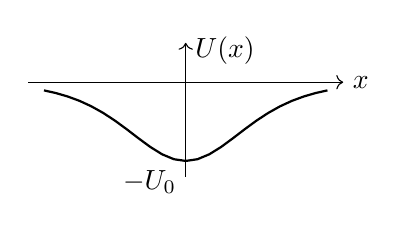
\begin{tikzpicture}
	\draw[->] (-2,0)--(2,0);
	\draw[->] (0,-1.2)--(0,0.5);
	\draw[ thick,domain =-1.8:1.8] plot(\x,{-1/( cosh(\x)*cosh(\x))}); 
	\coordinate[label=right:$ U(x) $](Ux) at (0,0.4);
	\coordinate[label=right:$ x $](x) at (2,0);
	\coordinate[label=below left:$ -U_0 $](-U0) at (0,-1);
	\end{tikzpicture}\caption{FIG. 4}\label{Fig.4}
\end{wrapfigure}
\[ \frac{\d}{\d\xi}\left[(1-\xi^2)\frac{\d\psi}{\d\xi} \right]+\left[s(s+1)-\frac{\epsilon^2}{1-\xi^2} \right]\psi=0. \]
This is the equation of the associated Legendre polynomials; it can be brought to hypergeometric form by making the substitution  
\[ \psi = (1 − \xi^2)^{\epsilon/2}w(\xi) \]  
and temporarily changing the variable to $ \frac{1}{2}(1 − ξ)=u $:
\[ u(1-u)w''+(\epsilon+1)(1-2u)w'-(\epsilon-s)(\epsilon+s+1)w=0. \]
The solution finite for $ \xi= 1 $ (i.e. for $ x = \infty $) is
\[ \psi=(1 − \xi^2)^{\epsilon/2}w(\xi)F[\epsilon-s,\epsilon+s+1,\epsilon-1,(1-\xi)/2]. \]
If $\psi$ remains finite for $ \xi= −1 $ (i.e. for $ x = -\inf $), we must have $\epsilon-s=-n$ where $ n = 0, 1, 2, \dots $; then $ F $ is a polynomial of degree $ n $, which is finite for $ \xi = −1 $. 

Thus the energy levels are determined by $\epsilon-s=-n$, or
\[ E_n=-\frac{\h^2\alpha^2}{8m}\left[ -(2n+1)+\sqrt{1+\frac{8mU_0}{\alpha^2\h^2}} \right]^2. \]
There is a finite number of levels, determined by the condition $ \epsilon>0 $, i.e. $ n < s $.}
\section{Motion in a homogeneous field}\label{Motion in a homogeneous field}
Let us consider the motion of a particle in a homogeneous external field. We take the direction of the field as the axis of $ x $; let $ F $ be the force acting on the particle in this field. In an electric field of intensity $ E $, this force is $ F = eE $, where $ e $ is the charge on the particle.

The potential energy of the particle in the homogeneous field is of the form $ U = −Fx+\mathrm{const} $; choosing the constant so that $ U = 0 $ for $ x = 0 $, we have $ U = -Fx $. Schr\"odinger's equation for this problem is
\begin{equation}\label{24.1}
\frac{\d^2\psi}{{\d x}^2}+\frac{2m}{\h}(E+Fx)\psi=0.
\end{equation}


Since $ U $ tends to $ + \infty $ as $ x \to- \infty $, and vice versa, it is clear that the energy levels form a continuous spectrum occupying the whole range of energy values $ E $ from $ -\infty $ to $ +\infty $. None of these eigenvalues is degenerate, and they correspond to motion which is finite towards $ x = -\infty $ and infinite towards $ x= +\infty $.

Instead of the coordinate $ x $, we introduce the dimensionless variable
\begin{equation}\label{24.2}
\xi=\left(x+\frac{E}{F} \right)\left(\frac{2mF}{\h}\right)^{1/3}.
\end{equation}
Equation \eqref{24.1} then takes the form
\begin{equation}\label{24.3}
\psi''+\xi\psi=0.
\end{equation}
This equation does not contain the energy parameter. Hence, if we obtain a solution of it which satisfies the necessary conditions of finiteness, we at once have the eigenfunction for arbitrary values of the energy.

The solution of equation \eqref{24.3} which is finite for all $ x $ has the form (see \S b of the Mathematical Appendices)
\begin{equation}\label{24.4}
\psi(\xi)=A\Phi(-\xi),
\end{equation}
where
\[ \Phi(\xi)=\frac{1}{\sqrt{\pi}}\int_{0}^{\infty}\cos\left(\frac{1}{3}u^3+u\xi\right)\d u \]
is called the \textit{Airy function}, while $ A $ is a normalization factor which we shall determine below.

As $ \xi\to-\infty $, the function $ \psi(\xi) $ tends exponentially to zero. The asymptotic expression which determines $ \psi(\xi) $ for large negative values of $\xi$ is (see (b.4))
\begin{equation}\label{24.5}
\psi(\xi)\approx\frac{A}{2|\xi|^{1/4}}\exp\left(-\frac{2}{3}|\xi|^{3/2}\right)
\end{equation}
For large positive values of $\xi$, the asymptotic expression for $ \psi(\xi) $ is (see (b.5))\footnote{It may be noted, by way of anticipation, that the asymptotic expressions \eqref{24.5} and \eqref{24.6} correspond to the quasi-classical expressions for the wave function in the classically inaccessible and accessible regions (\S47).}
\begin{equation}\label{24.6}
\psi(\xi)=\frac{A}{\xi^{1/4}}\sin\left(\frac{2}{3}\xi^{3/2}+\frac{\pi}{4}\right).
\end{equation}
Using the general rule \eqref{5.4} for the normalization of eigenfunctions of a continuous spectrum, let us reduce the function \eqref{24.4} to the form normalized by the delta function of energy, for which
\begin{equation}\label{24.7}
\int_{-\infty}^{+\infty}\psi(\xi)\psi(\xi')\d x\delta(E'-E).
\end{equation}
In \S\ref{General properties of motion in one dimension} we gave a simple method of determining the normalization coefficient by means of the asymptotic expression for the wave functions. Following this method, we represent the function \eqref{24.6} as the sum of two travelling waves:
\[ \psi(\xi)\approx\frac{A}{2\xi^{1/4}}\left\{\exp\left[\i\left(\frac{2}{3}\xi^{3/2}-\frac{\pi}{4} \right) \right]+\exp\left[-\i\left(\frac{2}{3}\xi^{3/2}-\frac{\pi}{4} \right) \right] \right\} .\]
The current density, calculated from each of these two terms, is
\[ v(\frac{A}{2\xi^{1/4}})^2=\sqrt{\frac{2}{m}\left(E+Fx \right)}\left(\frac{A}{2\xi^{1/4}} \right)^2=A^2\frac{(2\h F)^{1/3}}{4m^{2/3}}. \]
and equating this to $ 1/2\pi\h $ we find
\begin{equation}\label{24.8}
A=\frac{(2m)^{1/3}}{\pi^{1/2}F^{1/6\h^{2/3}}}.
\end{equation}






{\small 
\textbf{PROBLEM}


Determine the wave functions in the momentum representation for a particle in a homogeneous field.





SOLUTION. The Hamiltonian in the momentum representation is
\[ \hat{H}=\frac{p^2}{2m}-\i\h F\frac{\d}{\d p}, \]
so that Schr\"odinger's equation for the wave function $ a (p) $ has the form
\[ -\i\h F\frac{\d a}{\d p}+\left(\frac{p^2}{2m}-E \right)a. \]
Solving this equation, we find the required functions
\[ a_E(p)=\frac{1}{\sqrt{2\pi\h F}}\exp\left\{\frac{\i}{\h F}F\left(Ep-\frac{p^3}{6m} \right) \right\}. \]
These functions are normalized by the condition
\[ \int_{-\infty}^{+\infty}a^*_E(p)a_{E'}(p)\d p=\delta(E'-E). \]
}
\section{The transmission coefficient}\label{The transmission coefficient}
Let us consider the motion of particles in a field of the type shown in Fig. \ref{Fig.5}: $ U (x) $ increases monotonically from one constant limit ($ U = 0 $ as $ x →\to-\infty $) to another ($ U = U_0 $ as $ x\to +\infty $). According to classical mechanics, a particle of energy $ E < U_0 $ moving in such a field from left to right, on reaching such a “potential wall”, is reflected from it, and begins to move in the opposite direction; if, however, $ E > U_0 $, the particle continues to move in its original direction, though with diminished velocity. In quantum mechanics, a new\begin{wrapfigure}[]{l}[0cm]{0cm}
	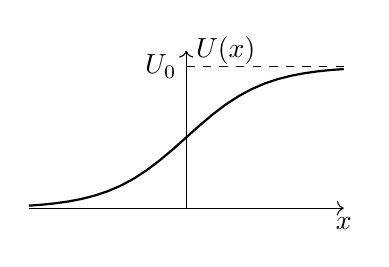
\begin{tikzpicture}
	\draw[->] (-2,0)--(2,0);
	\draw[->] (0,0)--(0,2);
	\draw[dashed] (0,1.8)--(2,1.8);
	\draw[ thick,domain =-2:2] plot(\x,{1.8/(1+exp(-2*\x)))});
	\coordinate[label=right:$ U(x) $](Ux) at (0,2);
	\coordinate[label=below:$ x $](x) at (2,0);
	\coordinate[label=left:$ U_0 $](U0) at (0,1.8);
	\end{tikzpicture}\caption{FIG. 5}\label{Fig.5}
\end{wrapfigure}
phenomenon appears: even for $ E > U_0 $, the particle may be reflected from the potential wall. The probability of reflection must in principle be calculated as follows.




Let the particle be moving from left to right. For large positive values of $ x $, the wave function must describe a particle which has passed “above the wall” and is moving in the positive direction of $ x $, i.e. it must have the asymptotic form
\begin{equation}\label{25.1}
\text{for }x\to\infty\colon\quad\psi\approx A\e^{\i k_2 x},\quad k_2=\frac{1}{\h}\sqrt{2m(E-U_0)}
\end{equation}
and $ A $ is a constant. To find the solution of Schr\"odinger's equation which satisfies this boundary condition, we calculate the asymptotic expression for $ x \to-\infty $; it is a linear combination of the two solutions of the equation of free motion, i.e. it has the form
\begin{equation}\label{25.2}
\text{for }x\to-\infty\colon\quad\psi\approx \e^{\i k_1 x}+B\e^{-k_1 x},\quad k_1=\frac{1}{\h}\sqrt{2mE}.
\end{equation}


The first term corresponds to a particle incident on the wall (we suppose $\psi$ normalized so that the coefficient of this term is unity); the second term represents a particle reflected from the wall. The probability current density in the incident wave is $ k_1 $, in the reflected wave $ k_1|B|^2 $, and in the transmitted wave $ k_2|A|^2 $. We define the \textit{transmission coefficient} $ D $ of the particle as the ratio of the probability current density in the transmitted wave to that in the incident wave:
\begin{equation}\label{25.3}
D=\frac{k_2}{k_1}|A|^2.
\end{equation}
Similarly we can define the reflection coefficient $ R $ as the ratio of the density in the reflected wave to that in the incident wave. Evidently $ R = 1 − D $:
\begin{equation}\label{25.4}
R=|B|^2=1-\frac{k_2}{k_1}|A|^2
\end{equation}
(this relation between $ A $ and $ B $ is automatically satisfied).

If the particle moves from left to right with energy $ E < U_0 $, then $ k_2 $ is purely imaginary, and the wave function decreases exponentially as $ x \to+\infty $. The reflected current is equal to the incident one, i.e. we have “total reflection” of the particle from the potential wall. We emphasize, however, that in this case the probability of finding the particle in the region where $ E < U $ is still different from zero, though it diminishes rapidly as $ x $ increases.

In the general case of an arbitrary stationary state (with energy $ E > U_0 $), the asymptotic form of the wave function is given, both for $ x \to-\infty $ and for $ x \to+\infty $, by a sum of waves propagated in each direction:
\begin{equation}\label{25.5}
\begin{split}
\psi&=A_1\e^{\i k_1x}+B_1\e^{-\i k_1x}\quad\text{for}\quad x\to-\infty,\\
\psi&=A_2\e^{\i k_2x}+B_2\e^{-\i k_2x}\quad\text{for}\quad x\to+\infty.
\end{split}
\end{equation}
Since these expressions are asymptotic forms of the same solution of a linear differential equation, there must be a linear relation between the coefficients $ A_1 $, $ B_1 $ and $ A_2 $, $ B_2 $. Let $ A_2 =\alpha A_1 + \beta B_1 $, where $\alpha$, $\beta$ are constants (in general complex) which depend on the specific form of the field $ U (x) $. The corresponding relation for $ B_2 $ can then be written down from the fact that Schr\"odinger's equation is real. This shows that, if $\psi$ is a solution of a given Schr\"odinger's equation, the complex conjugate function $\psi^*$ is also a solution. The asymptotic forms
\begin{equation*}
\begin{split}
\psi^*&=A_1^*\e^{-\i k_1x}+B_1^*\e^{\i k_1x}\quad\text{for}\quad x\to-\infty,\\
\psi^*&=A_2^*\e^{-\i k_2x}+B_2^*\e^{\i k_2x}\quad\text{for}\quad x\to+\infty
\end{split}
\end{equation*}
differ from \eqref{25.5} only in the nomenclature of the constant coefficients; we therefore have $ B_2^* = \alpha B_1^* + \beta A_1^* $ or $ B2 = \alpha^*B_1 + \beta^*A_1 $. Thus the coefficients in \eqref{25.5} are related by equations of the form
\begin{equation}\label{25.6}
A_2=\alpha A_1+\beta B_1,\quad B_2=\beta^*A_1+\alpha^*B_1.
\end{equation}


The condition of constant current along the $ x $-axis leads to the relation
\[ k_1(|A_1|^2-|B_1|^2)=k_2(|A_2|^2-|B_2|^2). \]
Expressing $ A_2 $, $ B_2 $ in terms of $ A_1 $, $ B_1 $ by \eqref{25.6}, we find
\begin{equation}\label{25.7}
|\alpha|^2-|\beta|^2=\frac{k_1}{k_2}.
\end{equation}


Using the relation \eqref{25.6}, we can show, in particular, that the reflection coefficients are equal (for a given energy $ E > U_0 $) for particles moving in the positive and negative directions of the $ x $-axis; the former case corresponds to putting $ B_2 = 0 $ in \eqref{25.5}, and the latter case to $ A_1 = 0 $. In these two cases, $ B_1/A_1 = −\beta^*/\alpha^* $ and $ A_2/B_2 = \beta/\alpha^* $ respectively. The corresponding reflection coefficients are
\[ R_1=\left|\frac{B_1}{A_1} \right|^2=\left|\frac{\beta^*}{\alpha^*}\right|^2,\quad R_2=\left|\frac{A_2}{B_2}\right|^2=\left|\frac{\beta}{\alpha^*}\right|^2 \]
whence it is clear that $ R_1 = R_2 $.

It is natural to call $ B_1/A_1 = -\beta^*/\alpha^* $ and $ A_2/B_2 = \beta/\alpha^* $ the \textit{reflection amplitudes} for motion in the positive and negative directions respectively. They are equal in modulus but may have different phase factors.





{\small
\textbf{PROBLEMS}


\textbf{1.} Determine the reflection coefficient of a particle from a rectangular potential wall (Fig. \ref{Fig.6}); the energy of the particle $ E > U_0 $.


\begin{wrapfigure}[]{l}[0cm]{0cm}
	\begin{tikzpicture}
	\draw[->] (-1,0)--(2.5,0);
	\draw[->] (0,0)--(0,2);
	\draw[thick] (-1,0)--(0,0)--(0,1.5)--(2,1.5);
	\coordinate[label=right:$ U(x) $](Ux) at (0,2);
	\coordinate[label=right:$ x $](x) at (2.5,0);
	\coordinate[label=left:$ U_0 $](U0) at (0,1.5);
	\end{tikzpicture}\caption{FIG. 6}\label{Fig.6}
\end{wrapfigure}






SOLUTION. Throughout the region $ x > 0 $, the wave function has the form \eqref{25.1}, while in the region $ x < 0 $ its form is \eqref{25.2}. The constants $ A $ and $ B $ are determined from the condition that $\psi$ and $\d\psi/\d x $ are continuous at $ x = 0 $:
\[ 1+B=A,\quad k_1(1-B)=k_2 A, \]
whence
\[ A=\frac{2k_1}{k_1+k_2},\quad B=\frac{k_1-k_2}{k_1+k_2}. \]
The reflection coefficient\footnote{In the limiting case of classical mechanics, the reflection coefficient must become zero. The expression obtained here, however, does not contain the quantum constant at all. This apparent contradiction is explained as follows. The classical limiting case is that in which the de Broglie wavelength of the particle $ \lambda\sim\h/p $ is small in comparison with the characteristic dimensions of the problem, i.e. the distances over which the field $ U (x) $ changes noticeably. In the schematic example considered, however, this distance is zero (at the point $ x = 0 $), so that the passage to the limit cannot be effected.} is \eqref{25.4}
\[ R=\left(\frac{k_1-k_2}{k_1+k_2} \right)^2\left(\frac{p_1-p_2}{p_1+p_2} \right)^2 \]
For $ E = U_0 $ ($ k_2 = 0 $), $ R $ becomes unity, while for $ E \to\infty $ it tends to zero as $ R=(U_0/4E)^2 $.





\textbf{2.} Determine the transmission coefficient for a rectangular potential barrier (Fig. \ref{Fig.7}).










SOLUTION. Let $ E $ be greater than $ U_0 $, and suppose that the incident particle is moving from left to right. Then we have for the wave function in the different regions expressions of the form
\begin{align*}
\psi&=\e^{\i k_1x}+A\e^{-\i k_1x}&\text{for }x&<0,\\
\psi&=B\e^{\i k_2 x}+B'\e^{-\i k_2x}&\text{for }0&<x<a,\\
\psi&=C\e^{\i k_1x}&\text{for }x&>a.
\end{align*}
(on the side $ x > a $ there can be only the transmitted wave, propagated in the positive direction of $ x $). The constants $ A $, $ B $, $ B' $ and $ C $ are determined from the
\begin{wrapfigure}[9]{r}[0cm]{0cm}
	\begin{tikzpicture}
	\draw[->] (-1.5,0)--(3,0);
	\draw[->] (0,0)--(0,2);
	\draw[thick] (-1.5,0)--(0,0)--(0,1.5)--(1.5,1.5)--(1.5,0)--(3,0);
	\coordinate[label=right:$ U(x) $](Ux) at (0,2);
	\coordinate[label=below:$ a $](a) at (1.5,0);
	\coordinate[label=left:$ U_0 $](U0) at (0,1.5);
	\end{tikzpicture}\caption{FIG. 7}\label{Fig.7}
\end{wrapfigure}
conditions of continuity of $\psi$ and $ \d\psi/\d x $ at the points $ x = 0 $ and $ a $. The transmission coefficient is determined as $ D = k_1|C|^2/k_1 = |C|^2 $. On calculating this, we obtain
\[ D=\frac{4k_1^2k_2^2}{(k_1^2-k_2^2)^2\sin^2ak_2+4k_1^2k_2^2} \]



For $ E < U_0 $, $ k_2 $ is a purely imaginary quantity; the corresponding expression for $ D $ is obtained by replacing $ k_2 $ by $ \i\varkappa_2 $ where $ \h\varkappa_2=\sqrt{2m(U_0-E)} $:
\[ D=\frac{4k_1^2\varkappa_2^2}{(k_1^2-\varkappa_2^2)^2\sin^2a\varkappa_2+4k_1^2\varkappa_2^2} \]




\textbf{3.} Determine the reflection coefficient for a potential wall defined by the formula 
\[ U (x) = U_0/(1 +\e^{-\alpha x}) \]
(Fig. \ref{Fig.5}); the energy of the particle is $ E > U_0 $.





SOLUTION. Schr\"odinger's equation is
\[ \frac{\d^2\psi}{{\d x}^2}+\frac{2m}{\h^2}\left(E-\frac{U_0}{1+\e^{-\alpha x}} \right)\psi=0. \]
We have to find a solution which, as $ x \to +\infty $, has the form
\[ \psi=\mathrm{const}\cdot\e^{\i k_2}. \]
We introduce a new variable
\[ \xi=-\e^{-\alpha x} .\]
(which takes values from $ -\infty $ to $ 0 $), and seek a solution of the form
\[ \psi=\xi^{-\i k_2/\alpha}w(\xi), \]
where $ w (\xi) $ tends to a constant as $ \xi\to 0 $ (i.e. as $ x \to\infty $). For $ w (\xi) $ we find an equation of hypergeometric type:
\[ \xi(1-\xi)w''+\left(1-\frac{2\i}{\alpha}k_2 \right)(1-\xi)w'+\frac{1}{\alpha^2}(k_2^2-k_1^2)w=0, \]
which has as its solution the hypergeometric function
\[ w=F\left[\frac{\i}{\alpha}(k_1-k_2),-\frac{\i}{\alpha}(k_1+k_2),-\frac{2\i}{\alpha}k_2+1,\xi \right] \]
(we omit a constant factor). As $ \xi\to0 $, this function tends to 1, i.e. it satisfies the condition imposed.

The asymptotic form of the function $\psi$ as $ \xi\to-\infty $ (i.e. $ x \to-\infty $) is\footnote{See formula (e.6), in each of whose two terms we must take only the first term of the expansion, i.e. replace the hypergeometric functions of $ 1/z $ by unity.
}
\begin{multline*}
\psi\approx\xi^{-\i k_2/\alpha}\left[C_1(-\xi)^{\i(k_2-k_1)/\alpha}+C_2(-\xi)^{\i(k_1+k_2)/\alpha} \right]=\\
=(-1)^{\i k_2/\alpha}\left[C_1\e^{\i k_1 x}+C_2^{-\i k_2 x} \right],
\end{multline*}
where
\begin{align*}
C_1&=\frac{\Gamma(-(2\i/\alpha)k_1)\Gamma(-(2\i/\alpha)k_2+1)}{\Gamma(-(\i/\alpha)(k_1+k_2))\Gamma(-(\i/\alpha)(k_1+k_2)+1)},\\
C_2&=\frac{\Gamma((2\i/\alpha)k_1)\Gamma(-(2\i/\alpha)k_2+1)}{\Gamma((\i/\alpha)(k_1-k_2))\Gamma((\i/\alpha)(k_1-k_2)+1)}.
\end{align*}
The required reflection coefficient is $ R = |C_2/C_1|^2 $ on calculating it by means of the well known formula
\[ \Gamma(x)\Gamma(1-x)=\frac{\pi}{\sin\pi x}, \]
we have
\[ R=\left\{\frac{\sinh\left[(\pi/\alpha)(k_1-k_2) \right]}{\sinh[(\pi/\alpha)(k_1+k_2)]} \right\}^2. \]
For $ E = U_0 $ ($ k_2 = 0 $), $ R $ becomes unity, while for $ E\to\infty $ it tends to zero as
\[ R=\left(\frac{\pi U_0}{\alpha\h} \right)^2\frac{2m}{E}\exp\left(-\frac{4\pi}{\alpha\h}\sqrt{2mE} \right). \]
In the limiting case of classical mechanics. $ R $ becomes zero, as it should.


\begin{wrapfigure}[6]{l}[0cm]{0cm}
	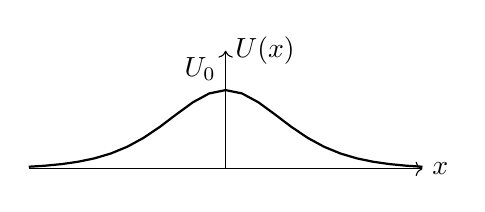
\begin{tikzpicture}
	\draw[->] (-2.5,0)--(2.5,0);
	\draw[->] (0,0)--(0,1.5);
	\draw[ thick,domain =-2.5:2.5] plot(\x,{1/(cosh(\x)*cosh(\x))))});
	\coordinate[label=right:$ U(x) $](Ux) at (0,1.5);
	\coordinate[label=right:$ x $](x) at (2.5,0);
	\coordinate[label=above left:$ U_0 $](U0) at (0,1);
	\end{tikzpicture}\caption{FIG. 8}\label{Fig.8}
\end{wrapfigure}




\textbf{4.} Determine the transmission coefficient for a potential barrier defined by the formula
\[ U(x)=\frac{U_0}{\cosh^2\alpha x} \]
(Fig. \ref{Fig.8}); the energy of the particle is $ E < U_0 $.






SOLUTION. The Schr\"odinger's equation is the same as that obtained in the solution of Problem 5, \S\ref{The linear oscillator}; it is necessary merely to alter the sign of $ U_0 $ and to regard the energy $ E $ now as positive. A similar calculation gives the solution
\begin{equation}\label{25-1}
\psi=(1-\xi^2)^{-\frac{\i k}{2\alpha}}F\left(-\frac{\i k}{\alpha}-s,-\frac{\i k}{\alpha}+s+1,-\frac{\i k}{\alpha}+1,\frac{1-\xi}{2} \right),\tag{1}
\end{equation}
where
\[ \xi=\tanh\alpha x,\quad k=\frac{1}{\h}\sqrt{2mE},\quad s=\frac{1}{2}\left(-1+\sqrt{1-\frac{8mU_0}{\alpha^2\h^2}} \right). \]
This solution satisfies the condition that, as $ x \to\infty $ (i.e. as $ \xi\to1$, $(1-\xi)\approx2\e^{-2\alpha x} $ ), the wave function should include only the transmitted wave ($ \sim\e^{\i kx} $). The asymptotic form of the wave function as $ x\to-\infty (\xi\to−1) $ is found by transforming the hypergeometric function with the aid of formula (e.7):
\begin{equation}\label{25-2}
\psi\sim\e^{\i kx}\frac{\Gamma(\i k/\alpha)\Gamma(1-\i k/\alpha)}{\Gamma(-s)\Gamma(1+s)}+\e^{\i kx}\frac{\Gamma(-\i k/\alpha)\Gamma(1-\i k/\alpha)}{\Gamma(-\i k/\alpha-s)\Gamma(-\i k/\alpha+s+1)}.\tag{2}
\end{equation}
Taking the squared modulus of the ratio of coefficients in this function, we obtain the following expression for the transmission coefficient $ D = 1 − R $:
\begin{align*}
D&=\frac{\sinh^2\frac{\pi k}{\alpha}}{\sinh^2\frac{\pi k}{\alpha}+\cos^2\left(\frac{\pi}{2}\sqrt{1-\frac{8mU_0}{\h^2\alpha^2}} \right)}\qquad\text{if}\quad\frac{8mU_0}{\h^2\alpha^2}<1,\\
D&=\frac{\sinh^2\frac{\pi k}{\alpha}}{\sinh^2\frac{\pi k}{\alpha}+\cosh^2\left(\frac{\pi}{2}\sqrt{\frac{8mU_0}{\h^2\alpha^2}-1} \right)}\qquad\text{if}\quad\frac{8mU_0}{\h^2\alpha^2}>1.
\end{align*}
The first of these formulae holds also for the case $ U_0 < 0 $, i.e. when the particle is passing over a potential well instead of a potential barrier. It is interesting to note that in that case $ D = 1 $ if $ 1 +8m|U_0|/\h^2\alpha^2 = (2n + 1)^2 $; thus, for certain values of the depth $ |U_0| $ of the well, particles passing over it are not reflected. This is evident from equation \eqref{25-2}, where the term in $ \e^{\i kx} $ vanishes for positive integral $ s $.





\textbf{5.} Determine how the transmission coefficient tends to zero as $ E \to0 $, assuming that the potential energy $ U (x) $ decreases rapidly at distances $ |x|\gg a $, where $ a $ is the dimension of the interaction region.





SOLUTION. For distances $ k |x| \ll1 $, $ E $ can be neglected in Schr\"odinger's equation. If also $ |x|\gg a $, the potential energy can also be neglected, and the equation becomes
\[ -\frac{\h^2}{2m}\frac{\d^2\psi}{{\d x}^2}=0, \]
the solution of this may be written as
\begin{equation}\label{25-3}
\psi=a_1+b_1x,\quad x<0,\qquad\psi=a_2+b_2x,\quad x>0.\tag{1}
\end{equation}

The relation between $ a_1 $, $ b_1 $ and $ a_2 $, $ b_2 $ can be found by solving the equation at distances $ |x|\sim a $. It is linear:
\begin{equation}\label{25-4}
a_1=\rho a_2+\mu b_2,\quad b_1=\nu a_1+\tau b_2.\tag{2}
\end{equation}
The coefficients $ \rho $, $ \mu $, $ \nu $ and $ \tau $ are real and independent of the energy, which does not appear in the equation.\footnote{Since the flux is constant, $ \rho\tau-\mu\nu= 1 $.
} The solution \eqref{25-3} must be the same as the first two terms in the expansion of \eqref{25.1} and \eqref{25.2} in powers of $ x $, so that
\[a_1=B+1,\quad b_1=\i k(1-B),\quad a_2=A,\quad b_2=\i kA. \]
Substituting these in \eqref{25-4} and solving for $ A $, we get, for small $ k\colon A \approx2\i k/\nu $, whence 
\[ D\approx\frac{4k^2}{\nu^2}\sim E \]
The transmission coefficient thus tends to zero in proportion to the particle energy. This is of course true for the examples in Problems 2 and 4.}
\chapter{ANGULAR MOMENTUM}
\section{Angular momentum}\label{Angular momentum}
IN \S\ref{Momentum}, to derive the law of conservation of momentum, we have made use of the homogeneity of space relative to a closed system of particles. Besides its homogeneity, space has also the property of isotropy: all directions in it are equivalent. Hence the Hamiltonian of a closed system cannot change when the system rotates as a whole through an arbitrary angle about an arbitrary axis. It is sufficient to require the fulfilment of this condition for an infinitely small rotation.


Let $\delta\bm{\phi}$ be the vector of an infinitely small rotation, equal in magnitude to the angle $\delta\phi$ of the rotation and directed along the axis about which the rotation takes place. The changes $\delta\bm{r}_a$ (in the radius vectors $ \bm{r}_a $ of the particles) in such a rotation are
\[ \delta\bm{r}_a=\delta\bm{\phi}\times\bm{r}_a. \]



An arbitrary function $ \psi(\bm{r}_1,\bm{r}_2,\dots) $ is thereby transformed into the function
\begin{multline*}
\psi(\bm{r}_1+\delta\bm{r}_1,\bm{r}_2+\delta\bm{r}_2,\dots)=\psi(\bm{r}_1+\bm{r}_2+\dots)+\sum_{a}\delta\bm{r}_a\cdot\nabla_a\psi=\\
=\psi(\bm{r}_1+\bm{r}_2+\dots)+\sum_{a}\delta\bm{\phi}\times\bm{r}_a\cdot\nabla_a\psi=\\
=\left(1+\delta\bm{\phi}\cdot\sum_{a}\bm{r}_a\times\nabla_a \right)\psi(\bm{r}_1+\bm{r}_2+\dots).
\end{multline*}
The expression
\[ 1+\delta\bm{\phi}\cdot\sum_{a}\bm{r}_a\times\nabla_a \]
is the operator of an infinitely small rotation. The fact that an infinitely small rotation does not alter the Hamiltonian of the system is expressed (cf. \S\ref{Momentum}) by the commutability of the “rotation operator” with the operator $ \hat{H} $. Since $\delta\bm{\phi}$ is a constant vector, this condition reduces to the relation
\begin{equation}\label{26.1}
\left(\sum_{a}\bm{r}_a\times\nabla_a\right)\hat{H}-\hat{H}\left(\sum_{a}\bm{r}_a\times\nabla_a\right)=0,
\end{equation}
which expresses a certain law of conservation.

The quantity whose conservation for a closed system follows from the property of isotropy of space is the \textit{angular momentum} of the system (cf. \textit{Mechanics}, \S9). Thus the operator $ \sum\bm{r}_a\times\nabla_a $ must correspond exactly, apart from a constant factor, to the total angular momentum of the system, and each of the terms $ \bm{r}_a\times\nabla_a $ of this sum corresponds to the angular momentum of an individual particle.

The coefficient of proportionality must be put equal to $ -\i\h $; then the expression for the angular momentum operator of a particle is $ -\i\h\bm{r}\times\nabla=\bm{r}\times\hat{\bm{p}} $ and corresponds exactly to the classical expression $ \bm{r}\times\bm{p} $. Henceforward we shall always use the angular momentum measured in units of $ \h $. The angular momentum operator of a particle, so defined, will be denoted by $ \hat{\bm{l}} $, and that of the whole system by $ \hat{\bm{L}} $. Thus the angular momentum operator of a particle is
\begin{equation}\label{26.2}
\h\hat{\bm{l}}=\bm{r}\times\hat{\bm{p}}=-\i\h\bm{r}\times\nabla
\end{equation}
or, in components,
\[ \h \hat{l_x}=y\hat{p}_z-z\hat{p}_y,\quad\hat{l_y}=z\hat{p}_x-x\hat{p}_z,\quad\hat{l_z}=x\hat{p}_y-y\hat{p}_x. \]


For a system which is in an external field, the angular momentum is in general not conserved. However, it may still be conserved if the field has a certain symmetry. Thus, if the system is in a centrally symmetric field, all directions in space at the centre are equivalent, and hence the angular momentum about this centre will be conserved. Similarly, in an axially symmetric field, the component of angular momentum along the axis of symmetry is conserved. All these conservation laws holding in classical mechanics are valid in quantum mechanics also.

In a system where angular momentum is not conserved, it does not have definite values in the stationary states. In such cases the mean value of the angular momentum in a given stationary state is sometimes of interest. It is easily seen that, in any non-degenerate stationary state, the mean value of the angular momentum is zero. For, when the sign of the time is changed, the energy does not alter, and, since only one stationary state corresponds to a given energy level, it follows that when $ t $ is changed into $ -t $ the state of the system must remain the same. This means that the mean values of all quantities, and in particular that of the angular momentum, must remain unchanged. But when the sign of the time is changed, so is that of the angular momentum, and we have $ \bar{\bm{L}}=-\bar{\bm{L}} $ , whence it follows that $ \bar{\bm{L}}=0 $. The same result can be obtained by starting from the mathematical definition of the mean value as being the integral of $\psi*\hat{\bm{L}}\psi$. The wave functions of non-degenerate states are real (see the end of \S\ref{The fundamental properties of Schr\"odinger's equation}). Hence the expression
\[ \bar{\bm{L}}=-\i\h\int\psi^*\left(\sum_{a}\bm{r}_a\times\nabla_a \right)\psi\d q \]
is purely imaginary, and since $ \bar{\bm{L}} $ must, of course, be real, it is evident that $ \bar{\bm{L}}=0 $.

Let us derive the rules for commutation of the angular momentum operators with those of coordinates and linear momenta. By means of the relations \eqref{16.2} we easily find
\begin{equation}\label{26.3}
\begin{split}
\{\hat{l}_x,x\}=0,\quad\{\hat{l}_x,y \}&=\i z,\quad\{\hat{l_x},z  \}=-\i y,\\
\{\hat{l}_y,y \}=0,\quad\{\hat{l}_y,z \}&=\i x,\quad\{\hat{l}_y,x  \}=-\i z,\\
\{\hat{l}_z,z \}=0,\quad\{\hat{l}_z,x \}&=\i y,\quad\{\hat{l}_z,y \}=-\i x.
\end{split}
\end{equation}
For instance,
\[ \hat{l}_xy-y\hat{l}_x=\frac{1}{\h}(y\hat{p}_z-z\hat{p_y})y-y(y\hat{p}_z-z\hat{p_y})\frac{1}{\h}=-\frac{z}{\h}{\hat{p}_y,y}=\i z \]




All the relations \eqref{26.3} can be written in tensor form as follows:
\begin{equation}\label{26.4}
\{\hat{l}_i,x_k\}=\i e_{ikl}x_l
\end{equation}
where $ e_{ikl} $ is the \textit{antisymmetric unit tensor} of rank three,\footnote{The antisymmetric unit tensor of rank three, $ e_{ikl} $ (also called the unit axial tensor), is defined as a tensor antisymmetric in all three suffixes, with $ e_{123} =1  $. It is evident that, of its $ 27 $ components, only $ 6 $ are not zero, namely those in which the suffixes $ i, k, l $ form some permutation of $ 1, 2, 3 $. Such a component is +1 if the permutation $ i, k, l $ is obtained from $ 1, 2, 3 $ by an even number of transpositions of pairs of figures, and is $ -1 $ if the number of transpositions is odd. Clearly 
\[ e_{ikl}e_{ikm} = 2\delta_{lm}, \quad e_{ikl}e_{ikl}= 6. \]	
The components of the vector $ \bm{C} = \bm{A} \times \bm{B} $ which is the vector product of the two vectors $ \bm{A} $ and $ \bm{B} $ can be written by means of the tensor $ e_{ikl} $ in the form
\[ C_i=e_{ikl}A_kB_l. \]
}and summation is implied over those suffixes which appear twice (called \textit{dummy suffixes}).

It is easily seen that a similar commutation rule holds for the angular momentum and linear momentum operators:
\begin{equation}\label{26.5}
\{\hat{l}_i,\hat{p}_k \}=\i e_{ikl}\hat{p}_l.
\end{equation}



By means of these formulae, it is easy to find the rules for commutation of the operators with one another. We have
\begin{multline*}
\h(\hat{l}_x\hat{l}_y-\hat{l}_y\hat{l}_x)=\hat{l}_x(z\hat{p}_x-x\hat{p}_z)-(z\hat{p}_x-x\hat{p}_z)\hat{l}_x=\\
=(\hat{l}_xz-z\hat{l}_x)\hat{p}_x-x(\hat{l}_x\hat{p}_z-\hat{p}_z\hat{l}_x)=\i y\hat{p}_x+\i x\hat{p}_y=\i\h\hat{l}_z.
\end{multline*}
Thus
\begin{equation}\label{26.6}
\{\hat{l}_y,\hat{l}_z  \}=\i\hat{l}_x,\quad\{\hat{l}_z,\hat{l}_x  \}=\i\hat{l}_y,\quad\{\hat{l}_x,\hat{l}_y  \}=\i\hat{l}_z,
\end{equation}
or
\begin{equation}\label{26.7}
\{\hat{l}_i,\hat{l}_k  \}=\i e_{ikl}\hat{l}_l
\end{equation}
Exactly the same relations hold for the operators of the total angular momentum of the system. For, since the angular momentum operators of different individual particles commute, we have, for instance,
\[ \sum_{a}\hat{l}_{ay}\sum_{a}\hat{l}_{az}-\sum_{a}\hat{l}_{az}\sum_{a}\hat{l}_{ay}=\sum_{a}\left(\hat{l}_{ay}\hat{l}_{az}-\hat{l}_{az}\hat{l}_{ay}  \right). \]
Thus
\begin{equation}\label{26.8}
\{\hat{L}_y,\hat{L}_z \}=\i\hat{L}_x,\quad\{\hat{L}_z,\hat{L}_x \}=\i\hat{L}_y,\quad\{\hat{L}_x,\hat{L}_y \}=\i\hat{L}_z.
\end{equation}
The relations \eqref{26.8} show that the three components of the angular momentum cannot simultaneously have definite values (except in the case where all three components simultaneously vanish: see below). In this respect the angular momentum is fundamentally different from the linear momentum, whose three components are simultaneously measurable.

From the operators $ \hat{L}_x,\hat{L}_y,\hat{L}_z $ we can form the operator of the square of the modulus of the angular momentum vector, and which we denote by :
\begin{equation}\label{26.9}
\hat{\bm{L}}^2=\hat{L}_x^2+\hat{L}_y^2+\hat{L}_z^2.
\end{equation}
This operator commutes with each of the operators :
\begin{equation}\label{26.10}
\{\hat{\bm{L}}^2,\hat{L}_x \}=0,\quad\{\hat{\bm{L}}^2,\hat{L}_y \}=0,\quad\{\hat{\bm{L}}^2,\hat{L}_z \}=0.
\end{equation}
Using \eqref{26.8}, we have
\[ \{\hat{L}_x^2,\hat{L}_z  \}=\hat{L}_x\{\hat{L}_x,\hat{L}_z \}+\{\hat{L}_x,\hat{L}_z \}\hat{L}_x=-\i\left(\hat{L}_x\hat{L}_y+\hat{L}_y\hat{L}_x \right) \]
\[ \{\hat{L}_y^2,\hat{L}_z  \}=\i\left(\hat{L}_x\hat{L}_y+\hat{L}_y\hat{L}_x \right)  \]
\[ \{\hat{L}_z^2,\hat{L}_z \}=0 \]
Adding these equations, we have $ \{\hat{\bm{L}}^2,\hat{L}_z  \}=0 $. Physically, the relations \eqref{26.10} mean that the square of the angular momentum, i.e. its modulus, can have a definite value at the same time as one of its components.

Instead of the operators $ \hat{L}_x,\hat{L}_y $ it is often more convenient to use the complex combinations
\begin{equation}\label{26.11}
\hat{L}_{+}=\hat{L}_x+\i\hat{L}_y,\quad\hat{L}_{-}=\hat{L}_x-\i\hat{L}_y
\end{equation}
It is easily verified by direct calculation using \eqref{26.8} that the following commutation rules hold:
\begin{equation}\label{26.12}
\{\hat{L}_{+},\hat{L}_{-}  \}=2\hat{L}_z,\quad\{\hat{L}_z,\hat{L}_{+} \}=\hat{L}_{+},\quad\{ 
\hat{L}_z,\hat{L}_{-} \}=-\hat{L}_{-},
\end{equation}
and it is also not difficult to see that
\begin{equation}\label{26.13}
\hat{\bm{L}}^2=\hat{L}_{+}\hat{L}_{-}+\hat{L}_z^2-\hat{L}_z=\hat{L}_{-}\hat{L}_{+}+\hat{L}_z^2+\hat{L}_z.
\end{equation}
Finally, we shall give some frequently used expressions for the angular momentum operator of a single particle in spherical polar coordinates. Defining the latter by means of the usual relations
\[ x=r\sin\theta\cos\phi,\quad y=r\sin\theta\sin\phi,\quad z=r\cos\theta, \]
we have after a simple calculation
\begin{equation}\label{26.14}
\hat{l}_z=-\i\frac{\p}{\p \phi},
\end{equation}
\begin{equation}\label{26.15}
\hat{l}_{\pm}=\e^{\pm\i\phi}\left(\pm\frac{\p}{\p\theta}+\i\cot\theta\frac{\p}{\p\phi} \right).
\end{equation}
Substitution in \eqref{26.13} gives the squared angular momentum operator of the particle:
\begin{equation}\label{26.16}
\hat{\bm{l}}^2=-\left[\frac{1}{\sin^2\theta}\frac{\p^2}{{\p\phi}^2}+\frac{1}{\sin\theta}\frac{\p}{\p\theta}\left(\sin\theta\frac{\p}{\p\phi} \right) \right]
\end{equation}
It should be noticed that this is, apart from a factor, the angular part of the Laplacian operator.





\section{Eigenvalues of the angular momentum}\label{Eigenvalues of the angular momentum}


In order to determine the eigenvalues of the component, in some direction, of the angular momentum of a particle, it is convenient to use the expression for its operator in spherical polar coordinates, taking the direction in question as the polar axis. According to formula \eqref{26.14}, the equation $ \hat{l}_z\psi=l_z\psi $ can be written in the form
\begin{equation}\label{27.1}
-\i\frac{\p\psi}{\p\phi}=l_z\psi.
\end{equation}
Its solution is
\[ \psi=f(r,\theta)\e^{\i l_z\phi}, \]
where $ f (r, \theta) $ is an arbitrary function of $ r $ and $ \theta $. If the function $\psi$ is to be single-valued, it must be periodic in $\phi$, with period $ 2\pi $. Hence we find\footnote{The customary notation for the eigenvalues of the angular momentum component is $ m $, which also denotes the mass of a particle, but this should not lead to any confusion.}
\begin{equation}\label{27.2}
l_z=m,\quad m=0,\pm 1,\pm 2,\dots
\end{equation}
Thus the eigenvalues $ l_z $ are the positive and negative integers, including zero. The factor depending on $\phi$, which characterizes the eigenfunctions of the operator $ \hat{l}_z $, is denoted by
\begin{equation}\label{27.3}
\Psi_m(\phi)=\frac{1}{\sqrt{2}}\e^{\i m\phi}.
\end{equation}
These functions are normalized so that
\begin{equation}\label{27.4}
\int_{0}^{2\pi}\Psi_m^*(\phi)\Psi_{m'}(\phi)\d\phi=\delta_{mm'}.
\end{equation}
The eigenvalues of the $ z $-component of the total angular momentum of the system are evidently also equal to the positive and negative integers:
\begin{equation}\label{27.5}
L_z=M,\quad M=0,\pm 1,\pm 2,\dots
\end{equation}
(this follows at once from the fact that the operator $ \hat{L}_z $ is equal to the sum of the commuting operators $ \hat{l}_z $ for the individual particles).

Since the direction of the $ z $-axis is in no way distinctive, it is clear that the same result is obtained for $ \hat{L}_x,\hat{L}_y $ and in general for the component of the angular momentum in any direction: they can all take integral values only. At first sight this result may appear paradoxical, particularly if we apply it to two directions infinitely close to each other. In fact, however, it must be remembered that the only common eigenfunction of the operators $ \hat{L}_x,\hat{L}_y,\hat{L}_z $ corresponds to the simultaneous values
\[ {L}_x={L}_y={L}_z=0; \]
in this case the angular momentum vector is zero, and consequently so is its projection upon any direction. If even one of the eigenvalues $ {L}_x,{L}_y,{L}_z $ is not zero, the operators $ \hat{L}_x,\hat{L}_y,\hat{L}_z $ have no common eigenfunctions. In other words, there is no state in which two or three of the angular momentum components in different directions simultaneously have definite values different from zero, so that we can say only that one of them is integral.

The stationary states of a system which differ only in the value of $ M $ have the same energy; this follows from general considerations, based on the fact that the direction of the $ z $-axis is in no way distinctive. Thus the energy levels of a system whose angular momentum is conserved (and is not zero) are always degenerate.\footnote{This is a particular case of the general theorem, mentioned in \S\ref{Stationary states}, which states that the levels are degenerate when two or more conserved quantities exist whose operators do not commute. Here the components of the angular momentum are such quantities.
}

Let us now look for the eigenvalues of the square of the angular momentum. We shall show how these values may be found, starting from the commutation rules \eqref{26.8} only. We denote by $\psi_M$ the wave functions of the stationary states with the same value of $ \bm{L}^2 $, belonging to one degenerate energy level, and distinguished by the value of $ M $.\footnote{Here it is supposed that there is no additional degeneracy leading to the same value of the energy for different values of the squared angular momentum. This is true for a discrete spectrum (except for the case of what is called \textit{accidental degeneracy} in a Coulomb field; see §36) and in general untrue for the energy levels of a continuous spectrum. However, even when such additional degeneracy is present, we can always choose the eigenfunctions so that they correspond to states with definite values of $ \bm{L}^2 $, and then we can choose from these the states with the same values of $ E $ and $ \hat{\bm{L}}^2 $. This is mathematically expressed by the fact that the matrices of commuting operators can always be simultaneously brought into diagonal form. In what follows we shall, in such cases, speak, for the sake of brevity, as if there were no additional degeneracy, bearing in mind that the results obtained do not in fact depend on this assumption, by what we have just said.}

First of all we note that, since the two directions of the $ z $-axis are physically equivalent, for every possible positive value $ M = |M| $ there is a corresponding negative value $ M = −|M| $. Let $ L $ (a positive integer or zero) denote the greatest possible value of $ |M| $ for a given $ \hat{\bm{L}}^2 $. The existence of this upper limit follows because is the operator $ \hat{\bm{L}}^2-\hat{L}_z^2=\hat{L}_x^2+\hat{L}_y^2 $ of the essentially positive physical quantity $ L_x^2 + L_y^2 $, and its eigenvalues therefore cannot be negative.

Applying the operator $ \hat{L}_z\hat{L}_{\pm} $ to the eigenfunction $\psi_M$ of the operator $ \hat{L}_z $ and using the commutation rule \ref{26.12}, we obtain
\begin{equation}\label{27.6}
\hat{L}_z\hat{L}_{\pm}\psi_M=(M+1)\hat{L}_{\pm}\psi_M.
\end{equation}
Hence we see that the function $ \hat{L}_{\pm}\psi_M $ is (apart from a normalization constant) the eigenfunction corresponding to the value $ M \pm 1 $ of the quantity $ L_z $:
\begin{equation}\label{27.7}
\psi_{M+1}=\mathrm{const}\cdot\hat{L}_{+}\psi_M,\quad\psi_{M-1}=\mathrm{const}\cdot L_-\psi_M.
\end{equation}
If we put $ M = L $ in the first of these equations, we must have identically
\begin{equation}\label{27.8}
\hat{L}_+\psi_L=0
\end{equation}
since there is by definition no state with $ M > L $. Applying the operator $ \hat{L}_- $ to this equation and using the relation \eqref{26.13}, we obtain
\[ \hat{L}_-\hat{L}_+\psi_L=(\hat{\bm{L}}^2-\hat{L}_z^2-\hat{L}_z)\psi_L=0. \]
Since, however, the $\psi_M$ are common eigenfunctions of the operators $ \hat{\bm{L}}^2 $ and $ \hat{L}_z $ , we have
\[ \hat{\bm{L}}^2\psi_L=\bm{L}^2\psi_L,\quad\hat{L}_z^2\psi_L=L^2\psi_L,\quad\hat{L}_z\psi_L=L\psi_L, \]
so that the equation found above gives
\begin{equation}\label{27.9}
\bm{L}^2=L(L+1).
\end{equation}


Formula \eqref{27.9} determines the required eigenvalues of the square of the angular momentum; the number $ L $ takes all positive integral values, including zero. For a given value of $ L $, the component $ L_z = M $ of the angular momentum can take the values
\begin{equation}\label{27.10}
M=L,L-1,\dots,-L,
\end{equation}
i.e. $ 2L + 1 $ different values in all. The energy level corresponding to the angular momentum $ L $ thus has $ (2 L + 1) $-fold degeneracy; this is usually called degeneracy with respect to the direction of the angular momentum. A state with angular momentum $ L = 0 $ (when all three components are also zero) is not degenerate. The wave function of such a state is spherically symmetric, as is evident from the fact that the change in it under any infinitesimal rotation, given by $ \hat{\bm{L}}\psi $, is in this case zero.

We shall often, for the sake of brevity, and in accordance with custom, speak of the “angular momentum” L of a system, understanding by this an angular momentum whose square is $ L (L + 1) $; the $ z $-component of the angular momentum is usually called just the “angular momentum component”.

The angular momentum of a single particle is denoted by the small letter $ l $, for which formula \eqref{27.9} becomes
\begin{equation}\label{27.11}
\bm{l}^2=l(l+1).
\end{equation}



Let us calculate the matrix elements of the quantities $ L_x $ and $ L_y $ in a representation in which $ L_z $ and $ \bm{L}^2 $, as well as the energy, are diagonal (M. Born, W. Heisenberg and P. Jordan 1926). First of all, we note that, since the operators $\hat{L}_x$ and $ \hat{L}_y $ commute with the Hamiltonian, their matrices are diagonal with respect to the energy, i.e. all matrix elements for transitions between states of different energy (and different angular momentum $ L $) are zero. Thus it is sufficient to consider the matrix elements for transitions within a group of states with different values of $ M $, corresponding to a single degenerate energy level.

It is seen from formulae \eqref{27.7} that, in the matrices of the operators $ \hat{L}_+ $ and $ \hat{L}_- $, only those elements are different from zero which correspond to transitions $ M - 1 \to M $ and $ M \to M - 1 $ respectively. Taking this into account, we find the diagonal matrix elements on both sides of the equation \eqref{26.13}, obtaining\footnote{In the symbols for the matrix elements, we omit for brevity all suffixes with respect to which they are diagonal (including $ L $).}
\[ L(L+1)=\langle M|L_+|M-1\rangle\langle M-1|L_-|M\rangle+M^2-M. \]
Noticing that, since the operators and are Hermitian,
\[\langle M-1|L_-|M\rangle={\langle M|L_+|M-1\rangle}^*  ,\]
we can rewrite this equation in the form
\[ |\langle M|L_+|M-1\rangle|^2=L(L+1)-M(M+1)=(L-M+1)(L+M), \]
whence\footnote{The choice of sign in this formula corresponds to the choice of the phase factors in the eigenfunctions of the angular momentum.
}
\begin{equation}\label{27.12}
\langle M|L_+|M-1\rangle=\langle M-1|L_-|M\rangle=\sqrt{(L+M)(L-M+1)}.
\end{equation}
Hence we have for the non-zero matrix elements of the quantities $ L_x $ and $ L_y $ themselves
\begin{equation}\label{27.13}
\begin{split}
\langle M|L_x|M-1\rangle&=\langle M-1|L_x|M\rangle=\frac{1}{2}\sqrt{(L+M)(L-M+1)},\\
\langle M|L_y|M-1\rangle&=-\langle M-1|L_y|M\rangle=-\frac{\i}{2}\sqrt{(L+M)(L-M+1)}.
\end{split}
\end{equation}


The diagonal elements in the matrices of the quantities $ L_x $ and $ L_y $ are zero. Since a diagonal matrix element gives the mean value of the quantity in the corresponding state, it follows that the mean values $\bar{{L}_x}$ and $ \bar{{L}_y} $ are zero in states having definite values of $ L_z $. Thus, if the angular-momentum component in a given direction in space has a definite value, the vector $\bar{\bm{L}}$ itself is in that direction.





\section{Eigenfunctions of the angular momentum}\label{Eigenfunctions of the angular momentum}


The wave function of a particle is not completely determined when the values of $ l $ and $ m $ are prescribed. This is seen from the fact that the expressions for the operators of these quantities in spherical polar coordinates contain only the angles $\theta$ and $\phi$, so that their eigenfunctions can contain an arbitrary factor depending on $ r $. We shall here consider only the angular part of the wave function which characterizes the eigenfunctions of the angular momentum, and denote this by $ Y_{lm} (\theta,\phi) $, with the normalization condition:
\[ \int|Y_{lm}|^2\d o=1, \]
where $ \d o = \sin\theta\d\theta\d\phi $ is an element of solid angle.

We shall see that the problem of determining the common eigenfunctions of the operators $\hat{\bm{l}}^2$ and $ \hat{l}_z $ admits of separation of the variables $\theta$ and $\phi$, and these functions can be sought in the form
\begin{equation}\label{28.1}
Y_{lm}=\Psi_m(\phi)\Theta_{lm}(\theta),
\end{equation}
where $ \Theta_m(\phi) $ are the eigenfunctions of the operator $\hat{l}_z$, which are given by formula \eqref{27.3}. Since the functions $\Theta_m$ are already normalized by the condition \eqref{27.4}, the $\Theta_{lm}$ must be normalized by the condition
\begin{equation}\label{28.2}
\int_{0}^{\pi}|\Theta_{lm}|^2\sin\theta\d\theta.
\end{equation}


The functions $ Y_{lm} $ with different $ l $ or $ m $ are automatically orthogonal:
\begin{equation}\label{28.3}
\int_{0}^{2\pi}\int_{0}^{\pi}Y_{l'm'}^*Y_{lm}\sin\theta\d\theta\d\phi=\delta_{ll'}\delta_{mm'},
\end{equation}
as being the eigenfunctions of angular momentum operators corresponding to different eigenvalues. The functions $\Psi_{m}(\phi)$ separately are themselves orthogonal (see \eqref{27.4}), as being the eigenfunctions of the operator $ \hat{l}_z $ corresponding to different eigenvalues $ m $ of this operator. The functions $\Theta_{lm}(\phi)$ are not themselves eigenfunctions of any of the angular momentum operators; they are mutually orthogonal for different $ l $, but not for different $ m $.

The most direct method of calculating the required functions is by directly solving the problem of finding the eigenfunctions of the operator $\hat{\bm{l}}^2$ written in spherical polar coordinates (formula \eqref{26.16}). The equation $ \hat{\bm{l}}^2\psi=\bm{l}^2\psi $ is:
\[ \frac{1}{\sin\theta}\frac{\p}{\p\theta}\left(\sin\theta\frac{\p\psi}{\p\theta} \right)+\frac{1}{\sin^2\theta}\frac{\p^2\psi}{{\p\phi}^2}+l(l+1)\psi=0. \]
Substituting in this equation the form \eqref{28.1} for $\psi$, we obtain for the function $\Theta_{lm}$ the equation
\begin{equation}\label{28.4}
\frac{1}{\sin\theta}\frac{\d}{\d\theta}\left(\sin\theta\frac{\d\Theta_{lm}}{\d\theta} \right)-\frac{m^2}{\sin^2\theta}\Theta_{lm}+l(l+1)\Theta_{lm}=0.
\end{equation}
This equation is well known in the theory of spherical harmonics. It has solutions satisfying the conditions of finiteness and single-valuedness for positive integral values of $ l \geqslant |m| $, in agreement with the eigenvalues of the angular momentum obtained above by the matrix method. The corresponding solutions are what are called \textit{associated Legendre polynomials} $ P_l^m(\cos\theta) $ (see \S c of the Mathematical Appendices). Using the normalization condition \eqref{28.2}, we find\footnote{The choice of the phase factor is not, of course, determined by the normalization condition. The definition (28.5) used in this book is the most natural from the viewpoint of the theory of addition of angular momenta. It differs by a factor il from the one usually adopted. The advantages of this choice will be clear from the footnotes in \S\S60, 106 and 107.}
\begin{equation}\label{28.5}
\Theta_{lm}=(-1)^m\i^l\sqrt{\frac{(2l+1)}{2}\frac{(l-m)!}{(l+m)!}}P_l^m(\cos\theta).
\end{equation}
Here it is supposed that $ m \geqslant0 $. For negative $ m $, we use the definition
\begin{equation}\label{28.6}
\Theta_{l,-|m|}=(-1)^m\Theta_{l|m|}
\end{equation}
In other words, $\Theta_{lm}$ for $ m < 0 $ is given by \eqref{28.5} with $ |m| $ instead of $ m $ and the factor $ (-1)^m $ omitted.

Thus the angular momentum eigenfunctions are mathematically just spherical harmonic functions normalized in a particular way. For reference, the complete expression embodying the above definitions is
\begin{equation}\label{28.7}
Y_{lm}(\theta,\phi)=(-1)^{(m+|m|)/2}\i^l\left[\frac{2l+1}{4\pi}\frac{(l-|m|)!}{(l+|m|)!} \right]^{1/2}P_l^{|m|}(\cos\theta)\e^{\i m\phi}.
\end{equation}
In particular,
\begin{equation}\label{28.8}
Y_{l0}=\i^l\sqrt{\frac{2l+1}{4\pi}}P_l(\cos\theta).
\end{equation}
It is evident that the functions differing in the sign of $ m $ are related by
\begin{equation}\label{28.9}
(-1)^{l-m}Y_{l,-m}=Y_{lm}^*.
\end{equation}


For $ l = 0 $ (so that $ m = 0 $ also) the spherical harmonic function reduces to a constant. In other words, the wave functions of the states of a particle with zero angular momentum depend only on $ r $, i.e. they have complete spherical symmetry, in agreement with the general statement in \S\ref{Eigenvalues of the angular momentum}.

For a given $ m $, the values of $ l $ starting from $ |m| $ denumerate the successive eigenvalues of the quantity $ \bm{l}^2 $ in order of increasing magnitude. Hence, from the general theory of the zeros of eigenfunctions (\S\ref{General properties of motion in one dimension}), we can deduce that the function $\Theta_{lm}$ becomes zero for $ l - |m| $ different values of the angle $\theta$; in other words, it has as nodal lines $ l - |m| $ “lines of latitude” on the sphere. If the complete angular functions are taken with the real factors $\cos m\phi$ or $ \sin m\phi $ instead of\footnote{Each such function corresponds to a state in which $ l_z $ does not have a definite value, but can have the values $\pm m$ with equal probability.} $ \e^{\pm\i|m|\phi} $, they have as further nodal lines $ |m| $ “lines of longitude”; the total number of nodal lines is thus $ l $.

Finally, we shall show how the functions $\Theta_{lm}$ may be calculated by the matrix method. This is done similarly to the calculation of the wave functions of an oscillator in \S\ref{The linear oscillator}. We start from the equation \eqref{27.8}:
\[ \hat{l}_+Y_{ll}=0. \]
Using the expression \eqref{26.15} for the operator $\hat{l}_+$ and substituting
\[ Y_{ll}=\frac{1}{\sqrt{2\pi}}\e^{\i l\phi}\Theta_{ll}(\theta), \]
we obtain for $\Theta_{ll}$ the equation
\[ \frac{\d\Theta_{ll}}{\d\theta}-l\cot\theta\cdot\Theta_{ll}=0, \]
whence $ \Theta_{ll} = \mathrm{const}\cdot\sin^l\theta $. Determining the constant from the normalization condition, we find
\begin{equation}\label{28.10}
\Theta_{ll}=(\i)^l\sqrt{\frac{(2l+1)!}{2}}\frac{1}{2^ll!}\sin^l\theta.
\end{equation}
Next, using \eqref{27.12}, we write
\[ \hat{l}_-Y_{l,m+1}=(l_-)_{m,m+1}Y_{lm}=\sqrt{(l-m)(l+m+1)}Y_{lm}. \]
A repeated application of this formula gives
\[ \sqrt{\frac{(l-m)!}{(l+m)!}}Y_{lm}=\frac{1}{\sqrt{(2l)!}}\hat{l}_-^{l-m}Y_{ll}. \]
The right-hand side of this equation is easily calculated by means of the expression \eqref{26.15} for the operator $\hat{l}_-$. We have
\[ \hat{l}_-\left[f(\theta)\e^{\i m\phi} \right]=\e^{\i(m-1)\phi}\sin^{1-m}\theta\frac{\d}{(\d\cos\theta)^{l-m}}\left(f\sin^m\theta \right) \]
A repeated application of this formula gives
\[ \hat{l}_-^{l-m}\e^{\i l\phi}\Theta_{ll}=\e^{\i m\phi}\sin^{-m}\theta\frac{\d^{l-m}}{(\d\cos\theta)^{l-m}}\left(\sin^l\theta\cdot\Theta_{ll} \right) .\]



Finally, using these relations and the expression \eqref{28.10} for $\Theta_{ll}$, we obtain the formula
\begin{equation}\label{28.11}
\Theta_{lm}(\theta)=(-\i)^l\sqrt{\frac{2l+1}{2}\frac{(l+m)!}{(l-m)!}}\frac{1}{2^ll!\sin^m\theta}\frac{\d^{l-m}}{(\d\cos\theta)^{l-m}}\sin^{2l}\theta,
\end{equation}
which is the same as \eqref{28.5}.





\section{Matrix elements of vectors}\label{Matrix elements of vectors}


Let us again consider a closed system of particles;\footnote{All the results in this section are valid also for a particle in a centrally symmetric field (and in general whenever the total angular momentum of the system is conserved).} let $ f $ be any scalar physical quantity characterizing the system, and $\hat{f}$ the operator corresponding to this quantity. Every scalar is invariant with respect to rotation of the coordinate system. Hence the scalar operator $\hat{f}$ does not vary when acted on by a rotation operator, i.e. it commutes with a rotation operator. We know, however, that the operator of an infinitely small rotation is the same, apart from a constant factor, as the angular momentum operator, so that
\begin{equation}\label{29.1}
\{\hat{f},\hat{\bm{L}} \}=0
\end{equation}
From the commutability of $\hat{f}$ with the angular momentum operator it follows that the matrix of $\hat{f}$ with respect to transitions between states with definite values of $ L $ and $ M $ is diagonal with respect to these suffixes. Moreover, since the specification of $ M $ defines only the orientation of the system relative to the axes of coordinates, and the value of a scalar is independent of this orientation, we can say that the matrix elements $ \langle n'LM|f|nLM\rangle $ are independent of the value of $ M $; $ n $ conventionally denotes all the quantum numbers other than $ L $ and $ M $ which define the state of the system. A formal proof of this assertion can be obtained from the commutativity of the operators $\hat{f}$ and $ \hat{L}_+ $:
\begin{equation}\label{29.2}
\hat{f}\hat{L}_+-\hat{L}_+\hat{f}=0.
\end{equation}
Let us write down the matrix element of this equation corresponding to the transition $ n, L, M \to n', L, M + 1 $. Taking into account the fact that the matrix of the quantity $ L_+ $ has only elements with $ n, L, M \to n, L, M + 1 $, we obtain
\begin{multline*}
\langle n',L,M+1|f|n,L,M+1\rangle\langle n,L,M+1|L_+|n,L,M\rangle=\\
=\langle n',L,M+1|L_+|n',L,M\rangle\langle n',L,M|f|n,L,M\rangle,
\end{multline*}
and since the matrix elements of the quantity $ L_+ $ are independent of the suffix $ n $, we find
\begin{equation}\label{29.3}
\langle n',L,M+1|f|n,L,M+1\rangle=\langle n',L,M|f|n,L,M\rangle,
\end{equation}
whence it follows that all the quantities $ \langle n', L, M| f|n, L, M\rangle $ for different $ M $ (the other suffixes being the same) are equal.

If we apply this result to the Hamiltonian itself, we obtain our previous result that the energy of the stationary states is independent of $ M $, i.e. that the energy levels have $ (2L + 1) $-fold degeneracy.

Next, let $ \bm{A} $ be some vector physical quantity characterizing a closed system. When the system of coordinates is rotated (and, in particular, in an infinitely small rotation, i.e. when the angular momentum operator is applied), the components of a vector are transformed into linear functions of one another. Hence, as a result of the commutation of the operators $\hat{L}_i$ with the operators $\hat{A}_i$, we must again obtain components of the same vector, $\hat{A}_i$. The exact form can be found by noticing that, in the particular case where $ \bm{A} $ is the radius vector of the particle, the formulae \eqref{26.4} must be obtained. Thus we find the commutation rules
\begin{equation}\label{29.4}
\{ \hat{L}_i,\hat{A}_k \}=\i e_{ikl}\hat{A}_l
\end{equation}


These relations enable us to obtain several results concerning the form of the matrices of the components of the vector $ \bm{A} $ (M. Born, W. Heisenberg and P. Jordan 1926). First of all, it is possible to derive selection rules which determine the transitions for which the matrix elements can be different from zero. We shall not go through the fairly lengthy calculations here, however, since it will appear later (\S107) that these rules are actually a direct consequence of the general transformation properties of vector quantities and can be derived from the latter with hardly any calculation at all. Here we shall merely give the rules, without proof.

The matrix elements of all the components of a vector can be different from zero only for transitions in which the angular momentum $ L $ changes by not more than one unit:
\begin{equation}\label{29.5}
L\to L,L+1
\end{equation}
There is a further selection rule which forbids transitions between any two states with $ L = 0 $. This rule is an obvious consequence of the complete spherical symmetry of states with angular momentum zero.

The selection rules for the angular momentum component $ M $ are different for the different components of a vector: the matrix elements can be different from zero for transitions where $ M $ changes as follows:
\begin{equation}\label{29.6}
\begin{split}
M\to M+1\quad\text{for}\quad &A_+=A_x+\i A_y,\\
M\to M-1\quad\text{for}\quad &A_-=A_z-\i A_y,\\
M\to M\quad\quad\text{for}\quad&A_z.
\end{split}
\end{equation}


Moreover, it is possible to determine a general form for the matrix elements of a vector as functions of the number $ M $. These important and frequently used formulae are given here, also without proof, since they are actually a particular case of more general relations derived in \S107 for any tensor quantities.

The non-zero matrix elements of the quantity $ A_z $ are given by the formulae
\begin{equation}\label{29.7}
\begin{split}
\langle n'LM|A_z|nLM\rangle&=\frac{M}{\sqrt{L(L+1)(2L+1)}}\langle n'L||A||nL\rangle,\\
\langle n'LM|A_z|n,L-1,M\rangle&=\sqrt{\frac{L^2-M^2}{L(2L-1)(2L+1)}}\langle n'L||A||n,L-1\rangle,\\
\langle n',L-1,M|A_z|nLM\rangle&=\sqrt{\frac{L^2-M^2}{L(2L-1)(2L+1)}}\langle n',L-1||A||nL\rangle.
\end{split}
\end{equation}
Here the symbol \[ \langle
 n'L'||A||nL\rangle \] 
denotes a \textit{reduced matrix element}, a quantity independent of the quantum number $ M $.\footnote{The appearance in formulae \eqref{29.7} and \eqref{29.9} of denominators which depend on $ L $ is in accordance with the general notation used in \S107. The convenience of these denominators is shown, in particular, by the simple form of equation \eqref{29.12} for the matrix elements of the scalar product of two vectors.
	

The symbol for the reduced matrix element is to be taken as a whole, in contrast to the matrix element symbol (see the comments following \eqref{11.17}).
} These matrix elements are related by
\begin{equation}\label{29.8}
\langle
n'L'||A||nL\rangle=\langle
nL||A||n'L'\rangle^*,
\end{equation}
which follows directly from the fact that the operator is $\hat{A}_z$ Hermitian.

The matrix elements of the quantities $ A_- $ and $ A_+ $ are also determined by the reduced matrix elements. The non-zero matrix elements of $ A_- $ are.
\begin{multline}\label{29.9}
\langle n',L,M-1|A_-|nLM\rangle=\sqrt{\frac{(L-M+1)(L+M)}{L(L+1)(2L+1)}}\langle n'L||A||nL\rangle,\\
\langle n',L,M-1|A_-|n,L-1,M\rangle=\sqrt{\frac{(L-M+1)(L-M)}{L(2L-1)(2L+1)}}\langle n'L||A||n,L-1\rangle,\\
\langle n',L-1,M-1|A_-|n,L,M\rangle=-\sqrt{\frac{(L+M-1)(L+M)}{L(2L-1)(2L+1)}}\langle n',L-1||A||n,L\rangle
\end{multline}
The matrix elements of $ A_+ $ need not be written out separately: since $ A_x $ and $ A_y $ are real we have
\begin{equation}\label{29.10}
\langle n'L'M'|A_+|nLM\rangle=\langle nLM|A_-|n'L'M'\rangle^*.
\end{equation}



There is a formula which expresses the matrix elements of the scalar $ \bm{A}\bm{B} $ in terms of the reduced matrix elements of the two vector quantities $ \bm{A} $ and $ \bm{B} $. The calculation is conveniently carried out by writing the operator $ \hat{\bm{A}}\hat{\bm{B}} $ in the form
\begin{equation}\label{29.11}
\hat{\bm{A}}\hat{\bm{B}}=\frac{1}{2}(\hat{A}_+\hat{B}_-+\hat{A}_-\hat{B}_+)+\hat{A}_z\hat{B}_z.
\end{equation}
The matrix of $ \bm{A}\bm{B} $ (like that of any scalar) is diagonal with respect to $ L $ and $ M $. A calculation by means of formulae \eqref{29.7}–\eqref{29.9} gives the result
\begin{equation}\label{29.12}
\langle n'LM|\bm{A}\bm{B}|nLM\rangle=\frac{1}{2L+1}\sum_{n'',L''}\langle n'L||A||n''L''\rangle\langle n''L''||B||nL\rangle,
\end{equation}
where $ L'' $ takes the values $ L, L\pm 1 $.

For reference, we shall give the reduced matrix elements for the vector $ \bm{L} $ itself. A comparison of \eqref{29.9} and \eqref{27.12} shows that
\begin{equation}\label{29.13}
\begin{split}
\langle L||L|L\rangle=\sqrt{L(L+1)(2L+1)},\\
\langle L-1||L||L\rangle=\langle L||L||L-1\rangle=0.
\end{split}
\end{equation}


A quantity that often occurs in applications is the unit vector $ \bm{n} $ along the radius vector of the particle. Its reduced matrix elements can be calculated by finding, for example, the matrix elements of $ n_z = \cos\theta $ for a zero angular-momentum component, $ m = 0 $;
\[ \langle l-1,0|n_z|l0\rangle=\int_{0}^{\pi}\Theta_{l-1,0}^*\cos\theta\cdot\Theta_{l0}\sin\theta\d\theta \]
with the functions $\Theta_{l0}$ given by \eqref{28.11}. The evaluation of the integral\footnote{By $ l-1 $ times integrating by parts with $ \d \cos\theta $; the general formula for integrals of this type is (107.14).} gives
\[ \langle l-1,0|n_z|l0\rangle=\frac{\i l}{\sqrt{(2l-1)(2l+1)}}. \]
The matrix elements for transitions $ l \to l $ are zero (as for any polar vector of an individual particle; see (30.8) below). Comparison with \eqref{29.7} then gives
\begin{equation}\label{29.14}
\langle l-1||n||l\rangle=-\langle l||n||l-1\rangle=\i\sqrt{l},\quad\langle l||n||l\rangle=0.
\end{equation}






{\small
\textbf{PROBLEM}


Average the tensor $ n_in_k-(1/3)\delta_{ik} $ (where $ \bm{n} $ is a unit vector along the radius vector of a particle) over a state where the magnitude but not the direction of the vector $ \bm{1} $ is given (i.e. $ l_z $ is indeterminate).





SOLUTION. The required mean value is an operator which can be expressed in terms of the operator $\hat{\bm{l}}$ alone. We seek it in the form
\[ \bar{n_in_k}-\frac{1}{3}\delta_{ik}=a\left[\hat{l}_i\hat{l}_k+\hat{l}_k\hat{l}_i-\frac{2}{3}\delta_{ik}l(l+1) \right]; \]
this is the most general symmetrical tensor of rank two with zero trace that can be formed from the components of $\hat{\bm{l}}$. To determine the constant a we multiply this equation on the left by $ \hat{l}_i $ and on the right by $\hat{l}_k$ (summing over $ i $ and $ k $). Since the vector $ \bm{n} $ is perpendicular to the vector $ \h\hat{\bm{l}}=\hat{\bm{r}
}\times\hat{\bm{p}} $, we have $ n_i\hat{l}_i=0 $. The product $ \hat{l}_i\hat{l}_i\hat{l}_k\hat{l}_k=(\hat{\bm{l}}^2)^2 $ is replaced by its eigenvalue $ l^2(l + 1)^2 $, and the product is transformed by means of the commutation relations \eqref{26.7} as follows:
\begin{multline*}
\hat{l}_i\hat{l}_k\hat{l}_i\hat{l}_k=\hat{l}_i\hat{l}_i\hat{l}_k\hat{l}_k-\i e_{ikl}\hat{l}_i\hat{l}_l\hat{l}_k=(\hat{\bm{l}})^2-\frac{\i}{2}e_{ikl}\hat{l}_i(\hat{l}_l\hat{l}_k-\hat{l}_k\hat{l}_l)=\\
=(\hat{\bm{l}})^2+\frac{1}{2}e_{ikl}e_{lkm}\hat{l}_i\hat{l}_m=(\hat{\bm{l}})^2-\hat{\bm{l}}^2=l^2(l+1)^2-l(l+1)
\end{multline*}
(using the fact that $ e_{ikl}e_{mkl} = 2\delta_{im} $). After a simple reduction we obtain the result
\[ a=-\frac{1}{(2l-1)(2l+3)}. \]}





\section{Parity of a state}\label{Parity of a state}


Besides the parallel displacements and rotations of the coordinate system, the invariance under which represents the homogeneity and isotropy of space respectively, there is another transformation which leaves unaltered the Hamiltonian of a closed system. This is what is called the \textit{inversion transformation}, which consists in simultaneously changing the sign of all the coordinates, i.e. a reversal of the direction of each coordinate axis; a right-handed coordinate system then becomes left-handed, and vice versa. The invariance of the Hamiltonian under this transformation expresses the symmetry of space under mirror reflections.\footnote{Invariance under inversion exists also for the Hamiltonian of a system of particles in a centrally symmetric field with the centre at the origin.
} In classical mechanics, the invariance of Hamilton’s function with respect to inversion does not lead to a conservation law, but the situation is different in quantum mechanics.

Let us denote by $\hat{P}$ (for “parity”) an inversion operator whose effect on a wave function $\psi(\bm{r})$ is to change the sign of the coordinates:
\begin{equation}\label{30.1}
\hat{P}\psi(\bm{r})=\psi(-\bm{r})
\end{equation}
It is easy to find the eigenvalues $ P $ of this operator, which are determined by the equation
\begin{equation}\label{30.2}
\hat{P}\psi(\bm{r})=P\psi(\bm{r})
\end{equation}
To do so, we notice that a double application of the inversion operator amounts to identity: the argument of the function is unchanged. In other words, we have $ \hat{P}^2\psi=P^2\psi=\psi $, i.e. $ P^2 = 1 $, whence
\begin{equation}\label{30.3}
P=\pm 1
\end{equation}
Thus the eigenfunctions of the inversion operator are either unchanged or change in sign when acted upon by this operator. In the first case, the wave function (and the corresponding state) is said to be \textit{even}, and in the second it is said to be \textit{odd}.

The invariance of the Hamiltonian under inversion (i.e. the fact that the operators $\hat{H}$ and $ \hat{P} $ commute) thus expresses the \textit{law of conservation of parity}: if the state of a closed system has a definite parity (i.e. if it is even, or odd) then this parity is conserved in the course of time.\footnote{To avoid misunderstanding, it should be mentioned that this refers to the non-relativistic theory. There exist interactions in Nature, falling in the realm of relativistic theory, which violate the conservation of parity.
}

The angular momentum operator also is invariant under inversion, which changes the sign of the coordinates and of the operators of differentiation with respect to them; the operator \eqref{26.2} thus remains unaltered. In other words, the inversion operator commutes with the angular momentum operator, and this means that the system can have a definite parity simultaneously with definite values of the angular momentum $ L $ and its component $ M $. All states that differ only in the value of $ M $ have the same parity; this is evident because the properties of a closed system are independent of its orientation in space, and it can be formally demonstrated from the commutation rule $ \hat{L}_+\hat{P}-\hat{P}\hat{L}_+ $ by the same method as in deriving \eqref{29.3} from \eqref{29.2}.

There are specific \textit{parity selection rules} for the matrix elements of various physical quantities. Let us first consider scalars. Here we must distinguish \textit{true scalars}, which are unchanged by inversion, from \textit{pseudoscalars}, which change sign, for instance the scalar product of an axial and a polar vector The operator of a true scalar $ f $ commutes with $\hat{P}$; hence it follows that, if the matrix of $ P $ is diagonal, then the matrix of $ f $ is diagonal also as regards the parity suffix, i.e. the matrix elements are zero except for transitions $ g \to g $ and $ u \to u $ (where $ g $ and $ u $ denote even and odd states respectively). For the operator of a pseudoscalar quantity, we have $ \hat{P}\hat{f}=-\hat{f}\hat{P} $; the operators $ \hat{P} $ and $\hat{f}$ \textit{anticommute}. The matrix element of this equation for a transition $ g \to g $ is \[ P_{gg}f_{gg} = - f_{gg}P_{gg}, \] and so $ f_{gg} = 0 $ since $ P_{gg} = 1 $. Similarly we find that $ f_{uu} = 0 $. Thus, in the matrix of a pseudoscalar quantity, only those elements can be different from zero which correspond to transitions with change of parity. The selection rules for the matrix elements of scalars are therefore:
\begin{equation}\label{30.4}
\begin{split}
\text{true scalars}\qquad g\to g,u\to u;\\
\text{pseudoscalars}\qquad g\to u,u\to g.
\end{split}
\end{equation}



These rules can also be obtained directly from the definition of the matrix elements. Let us consider, for example, the integral $ f_{ug}=\int\psi_u^*\hat\psi_g\d q $, where the function $\psi_g$ is even and $\psi_u$ odd. When all the coordinates change sign, the integrand does so if $ f $ is a true scalar; on the other hand, the integral taken over all space cannot change when the variables of integration are renamed. Hence it follows that $ f_{ug} = - f_{ug} $, i.e. $ f_{ug} \equiv 0 $.

We can similarly derive selection rules for vector quantities. Here it must be recalled that ordinary (polar) vectors change sign on inversion, while axial vectors (such as the angular momentum vector, which is the vector product of the two polar vectors $ \bm{p} $ and $ \bm{r} $) are unchanged by inversion. The selection rules are found to be:
\begin{equation}\label{30.5}
\begin{split}
\text{polar vectors}\qquad g\to u,u\to g;\\
\text{axial vectors}\qquad g\to g,u\to u.
\end{split}
\end{equation}
Let us determine the parity of the state of a single particle with angular momentum $ l $. The inversion transformation ($ x \to-x, y \to-y, z \to-z $) is, in spherical polar coordinates, the transformation
\begin{equation}\label{30.6}
r\to r,\quad\theta\to\pi-\theta,\quad\phi\to\phi+\pi.
\end{equation}
The dependence of the wave function of the particle on the angle is given by the spherical harmonic $ Y_{lm} $, which, apart from a constant that is here unimportant, has the form $ P_l^m(\cos\theta)\e^{\i m\phi} $. When $\phi$ is replaced by $ \phi+\pi $, the factor $ \e^{\i m\phi} $ is multiplied by $ (-1)^m $, and when $\theta$ is replaced by $ \pi-\theta $, $ P_l^m(\cos\theta) $ becomes $ P_l^m(-\cos\theta)=(-1)^{l-m}P_l^m(\cos\theta) $. Thus the whole function is multiplied by $ (-1)^l $ (independent of $ m $, in agreement with what was said above), i.e. the parity of a state with a given value of $ l $ is
\begin{equation}\label{30.7}
P=(-1)^l.
\end{equation}
We see that all states with even $ l $ are even, and all those with odd $ l $ are odd.

A vector physical quantity relating to an individual particle can have non-zero matrix elements only for transitions with $ l \to l $ or $ l \pm 1 $ (\S\ref{Matrix elements of vectors}). Remembering this, and comparing formula \eqref{30.7} with what was said above regarding the change of parity in the matrix elements of vectors, we reach the result that the matrix elements of vectors relating to an individual particle are zero except for the transitions:
\begin{equation}\label{30.8}
\begin{split}
\text{polar vectors}\qquad l&\to l\pm 1,\\
\text{axial vectors}\qquad l&\to 1.
\end{split}
\end{equation}






\section{Addition of angular momenta}\label{Addition of angular momenta}


Let us consider a system composed of two parts whose interaction is weak. If the interaction is entirely neglected, then for each part the law of conservation of angular momentum holds. The angular momentum $ \bm{L} $ of the whole system can be regarded as the sum of the angular momenta $ \bm{L}_1 $ and $ \bm{L}_2 $ of its parts. In the next approximation, when the weak interaction is taken into account, $ \bm{L}_1 $ and $ \bm{L}_2 $ are not exactly conserved, but the numbers $ L_1 $ and $ L_2 $ which determine their squares remain “good” quantum numbers suitable for an approximate description of the state of the system. Regarding the angular momenta in a classical manner, we can say that in this approximation $ \bm{L}_1 $ and $ \bm{L}_2 $ rotate round the direction of L while remaining unchanged in magnitude.

For such systems the question arises regarding the “law of addition” of angular momenta: what are the possible values of $ L $ for given values of $ L_1 $ and $ L_2 $? The law of addition for the components of angular momentum is evident: since $ \hat{L}_z=\hat{L}_{1z}+\hat{L}_{2z} $, it follows that
\begin{equation}\label{31.1}
M=M_1+M_2
\end{equation}
There is no such simple relation for the operators of the squared angular momenta, however, and to derive their “law of addition” we reason as follows.

If we take the quantities $ \bm{L}_1^2 ,  \bm{L}_2^2 ,  L_{1z} ,  L_{2z} $ as a complete set of physical quantities,\footnote{Together with such other quantities as form a complete set when combined with these four. These other quantities play no part in the subsequent discussion, and for brevity we shall ignore them entirely, and conventionally call the above four quantities a complete set.
} every state will be determined by the values of the numbers $ L_1, L_2, M_1, M_2 $. For given $ L_1 $ and $ L_2 $, the numbers $ M_1 $ and $ M_2 $ take $ (2L_1+1) $ and $ (2L_2 + 1) $ different values respectively, so that there are altogether $ (2L_1 + 1) (2L_2+1) $ different states with the same $ L_1 $ and $ L_2 $. We denote the wave functions of the states for this representation by $\phi_{L_1L_2M_1M_2}$.

Instead of the above four quantities, we can take the four quantities $ \bm{L}_1^2, \bm{L}_2^2, \bm{L}^2, L_z $ as a complete set. Then every state is characterized by the values of the numbers $ L_1, L_2, L, M $ (we denote the corresponding wave functions by $\psi_{L_1L_2M_1M_2}$). For given $ L_1 $ and $ L_2 $, there must of course be $ (2L_1 + 1)(2L_2 + 1) $ different states as before, i.e. for given $ L_1 $ and $ L_2 $ the pair of numbers $ L $ and $ M $ must take $ (2L_1 + 1)(2L_2 + 1) $ pairs of values. These values can be determined as follows.

By adding the various possible values of $ M_1 $ and $ M_2 $, we get the corresponding values of $ M $, as shown below:

\[ \begin{tabularx}{0.5\textwidth}{XXX}
$ M_1 $ & $ M_2 $ & $ M $\\
\hline
$ L_1 $ & $ L_2 $ & $ L_1+L_2 $\\
$ L_1 $ & $ L_2-1 $ & $ L_1+L_2-1 $\\
$ L_1-1 $ & $ L_2 $ & $ L_1+L_2-1 $\\
$ L_1-1 $ & $ L_2-1 $ & $ L_1+L_2-2 $\\
$ L_1 $ & $ L_2-2 $ & $ L_1+L_2-2 $\\
$ L_1-2 $ & $ L_2 $ & $ L_1+L_2-2 $\\
\dots &\dots&\dots\\
\end{tabularx}
 \]




We see that the greatest possible value of $ M $ is $ M = L_1 + L_2 $, corresponding to one state $\phi$ (one pair of values of $ M_1 $ and $ M_2 $). The greatest possible value of $ M $ in the states $\psi$, and hence the greatest possible value of $ L $ also, is therefore $ L_1 + L_2 $. Next, there are two states $\phi$ with $ M = L_1 + L_2 - 1 $. Consequently, there must also be two states $\psi$ with this value of $ M $; one of them is the state with $ L = L_1 + L_2 $ (and $ M = L - 1 $), and the other is that with $ L = L_1 + L_2 - 1 $ (and $ M = L $). For the value $ M = L_1 + L_2-2 $ there are three different states $\phi$. This means that, besides the values $ L = L_1 + L_2, L = L_1 + L_2 - 1 $, the value $ L = L_1 + L_2 - 2 $ can occur.

The argument can be continued in this way so long as a decrease of $ M $ by $ 1 $ increases by $ 1 $ the number of states with a given $ M $. It is easily seen that this is so until $ M $ reaches the value $ |L_1 - L_2| $. When $ M $ decreases further, the number of states no longer increases, remaining equal to $ 2L_2 + 1$ (if $ L_2 \leqslant L_1 $) . Thus $ |L_1 - L_2| $ is the least possible value of $ L $, and we arrive at the result that, for given $ L_1 $ and $ L_2 $, the number $ L $ can take the values
\begin{equation}\label{31.2}
L=L_1+L_2,L_1+L_2-1,\dots,|L_1-L_2|,
\end{equation}
that is $ 2L_2 + 1 $ different values altogether (supposing that $ L_2 \leqslant L_1 $). It is easy to verify that we do in fact obtain $ (2L_1 + 1)(2L_2+1) $ different values of the pair of numbers $ M $, $ L $. Here it is important to note that, if we ignore the $ 2L + 1 $ values of $ M $ for a given $ \hat{L} $, then only one state will correspond to each of the possible values \eqref{31.2} of $ L $.

This result can be illustrated by means of what is called the \textit{vector model}. If we take two vectors $ \bm{L}_1, \bm{L}_2 $ of lengths $ L_1 $ and $ L_2 $, then the values of $ L $ are represented by the integral lengths of the vectors $ \bm{L} $ which are obtained by vector addition of $ \bm{L}_1 $ and $ \bm{L}_2 $; the greatest value of $ L $ is $ L_1 + L_2 $, which is obtained when $ \bm{L}_1 $ and $ \bm{L}_2 $ are parallel, and the least value is $ |L_1 - L_2| $, when $ \bm{L}_1 $ and $ \bm{L}_2 $ are antiparallel.

In states with definite values of the angular momenta $ L_1 $, $ L_2 $ and of the total angular momentum $ L $, the scalar products $ \bm{L}_1\bm{L}_2 $, $ \bm{L}\bm{L}_1 $ and $ \bm{L}\bm{L}_2 $ also have definite values. These values are easily found. To calculate $ \bm{L}_1\bm{L}_2 $, we write $ \hat{\bm{L}}=\hat{\bm{L}}_1+\hat{\bm{L}}_2 $ or, squaring and transposing,
\[ 2\hat{\bm{L}}_1\hat{\bm{L}}_2=\hat{\bm{L}}^2-\hat{\bm{L}}_1^2-\hat{\bm{L}}_2^2. \]
Replacing the operators on the right-hand side of this equation by their eigenvalues, we obtain the eigenvalue of the operator on the left-hand side:
\begin{equation}\label{31.3}
\bm{L}_1\bm{L}_2=\frac{1}{2}\{ L(L+1)-L_1(L_1+1)-L_2(L_2+1) \}.
\end{equation}
Similarly we find
\begin{equation}\label{31.4}
\bm{L}\bm{L}_1=\frac{1}{2}\{L(L+1)+L_1(L_1+1)-L_2(L_2+1) \}
\end{equation}



Let us now determine the “addition rule for parities”. The wave function $\Psi$ of a system consisting of two independent parts is the product of the wave functions $\psi_1$ and $\Psi_2$ of these parts. Hence it is clear that if the latter are of the same parity (i.e. both change sign, or both do not change sign, when the sign of all the coordinates is reversed), then the wave function of the whole system is even. On the other hand, if $\Psi_1$ and $\Psi_2$ are of opposite parity, then the function $\Psi$ is odd. These statements may be written
\begin{equation}\label{31.5}
P=P_1P_2
\end{equation}
where $ P $ is the parity of the whole system and $ P_1 $, $ P_2 $ those of its parts. This rule can, of course, be generalized at once to the case of a system composed of any number of non-interacting parts.

In particular, if we are concerned with a system of particles in a centrally symmetric field (the mutual interaction of the particles being supposed weak), then the parity of the state of the whole system is given by
\begin{equation}\label{31.6}
P=(-1)^{l_1+l_2+\dots}
\end{equation}
see \eqref{30.7}. We emphasize that the exponent here contains the algebraic sum of the angular momenta $ l_i $, and this is not in general the same as their “vector sum”, i.e. the angular momentum $ L $ of the system.

If a closed system disintegrates (under the action of internal forces), the total angular momentum and parity must be conserved. This circumstance may render it impossible for a system to disintegrate, even if this is energetically possible.

For instance, let us consider an atom in an even state with angular momentum $ L = 0 $, which is able, so far as energy considerations go, to disintegrate into a free electron and an ion in an odd state with the same angular momentum $ L = 0 $. It is easy to see that in fact no such disintegration can occur (it is, as we say, \textit{forbidden}). For, by virtue of the law of conservation of angular momentum, the free electron would also have to have zero angular momentum, and therefore be in an even state $ (P = (−1)^0 = + 1) $; the state of the system ion$ + $electron would then be odd, however, whereas the original state of the atom was even.

\chapter{MOTION IN A CENTRALLY SYMMETRIC FIELD}\label{MOTION IN A CENTRALLY SYMMETRIC FIELD}
\section{Motion in a centrally symmetric field}\label{Motion in a centrally symmetric field}
\section{Spherical waves}\label{Spherical waves}
\section{Resolution of a plane wave}\label{Resolution of a plane wave}
\section{Fall of a particle to the centre}\label{Fall of a particle to the centre}
\section{Motion in a Coulomb field (spherical polar coordinates)}\label{Motion in a Coulomb field (spherical polar coordinates)}
\section{Motion in a Coulomb field (parabolic coordinates)}\label{Motion in a Coulomb field (parabolic coordinates)}
\chapter{PERTURBATION THEORY}\label{PERTURBATION THEORY}
\section{Perturbations independent of time}\label{Perturbations independent of time}
THE exact solution of Schr\"odinger’s equation can be found only in a comparatively small number of the simplest cases. The majority of problems in quantum mechanics lead to equations which are too complex to be solved exactly. Often, however, quantities of different orders of magnitude appear in the conditions of the problem; among them there may be small quantities such that, when they are neglected, the problem is so much simplified that its exact solution becomes possible. In such cases, the first step in solving the physical problem concerned is to solve exactly the simplified problem, and the second step is to calculate approximately the errors due to the small terms that have been neglected in the simplified problem. There is a general method, of calculating these errors; it is called \textit{perturbation theory}.

Let us suppose that the Hamiltonian of a given physical system is of the form
\[ \hat{H}=\hat{H}_0+\hat{V} \]
where $\hat{V}$ is a small correction (or \textit{perturbation}) to the \textit{unperturbed} operator $\hat{H}_0$ In \S\S\ref{Perturbations depending on time}, \ref{The secular equation} we shall consider perturbations $\hat{V}$ which do not depend explicitly on time (the same is assumed regarding $\hat{H}_0$ also). The conditions which are necessary for it to be permissible to regard the operator $\hat{V}$ as “small” compared with the operator $\hat{H}$ will be derived below.

The problem of perturbation theory for a discrete spectrum can be formulated as follows. It is assumed that the eigenfunctions $\psi_n^{(0)}$ and eigenvalues $ E_n^{(0)} $ of the discrete spectrum of the unperturbed operator $\hat{H}_0$ are known, i.e. the exact solutions of the equation
\begin{equation}\label{38.1}
\hat{H}_0\psi^{(0)}=E^{(0)}\psi^{(0)}
\end{equation}
are known. It is desired to find approximate solutions of the equation
\begin{equation}\label{38.2}
\hat{H}\psi=(\hat{H}_0+\hat{V})\psi=E\psi,
\end{equation}
i.e. approximate expressions for the eigenfunctions $\psi_n$ and eigenvalues $ E_n $ of the perturbed operator $\hat{H}$.

In this section we shall assume that no eigenvalue of the operator $ \hat{H}_0 $ is degenerate. Moreover, to simplify our results, we shall at first suppose that there is only a discrete spectrum of energy levels.

The calculations are conveniently performed in matrix form throughout.

To do this, we expand the required function $\psi$ in terms of the functions $ \psi_n^{(0)} $:
\begin{equation}\label{38.3}
\psi=\sum_mc_m\psi_m^{(0)},
\end{equation}
Substituting this expansion in \eqref{38.2} we obtain
\[ \sum_mc_m(E_m^{(0)}+\hat{V})\psi_m^{(0)}=\sum_mc_mE\psi_m^{(0)}; \]
multiplying both sides of this equation by $\psi_k^{(0)*}$ and integrating, we find
\begin{equation}\label{38.4}
(E-E_k^{(0)})c_k=\sum_mV_{km}c_m.
\end{equation}


Here we have introduced the matrix $ V_{km} $ of the perturbation operator $\hat{V}$, defined with respect to the unperturbed functions $\psi_m^{(0)}$:
\begin{equation}\label{38.5}
V_{km}=\int\psi_k^{(0)*}\hat{V}\psi_m^{(0)}\d q.
\end{equation}


We shall seek the values of the coefficients $ c_m $ and the energy $ E $ in the form of series
\[ E=E^{(0)}+E^{(1)}+\dots,\quad c_m=c_m^{(0)}+c_m^{(1)}+c_m^{(2)}+\dots, \]
where the quantities $ E^{(1)} $ and $ c_m^{(1)} $ are of the same order of smallness as the perturbation $\hat{V}$, the quantities $ E^{(2)} $ and $ c_m^{(2)} $ are of the second order of smallness, and so on.

Let us determine the corrections to the $ n $th eigenvalue and eigenfunction, putting accordingly $ c_n^{(0)} = 1 $, $ c_n^{(0)} = 0 $ for $ m \neq n $. To find the first approximation, we substitute in equation \eqref{38.4} $ E = E_n^{(0)} + E_n^{(1)} $, $ c_k = c_k^{(0)}+c_k^{(1)} $, and retain only terms of the first order. The equation with $ k = n $ gives
\begin{equation}\label{38.6}
E_n^{(1)}=V_{nn}=\int\psi_n^{(0)*}\hat{V}\psi_n^{(0)}\d q.
\end{equation}
Thus the first-order correction to the eigenvalue $ E_n^{(0)} $ is equal to the mean value of the perturbation in the state $  \psi_n^{(0)} $.

The equation \eqref{38.4} with $ k \ne n $ gives
\begin{equation}\label{38.7}
c_k^{(1)}=\frac{V_{kn}}{E_n^{(0)}-E_k^{(0)}},k\ne n,
\end{equation}
while $ c_n^{(1)} $ remains arbitrary; it must be chosen so that the function $ \psi_n = \psi_n^{(0)} + \psi_n^{(1)} $ is normalized up to and including terms of the first order. For this we must put $ c_n^{(1)} = 0 $. For the functions
\begin{equation}\label{38.8}
\psi_n^{(1)}={\sum_{m}}'\frac{V_{mn}}{E_n^{(0)}-E_m^{(0)}}\psi_m^{(0)}
\end{equation}
(the prime means that the term with $ m = n $ is omitted from the sum) are orthogonal to $\psi_n^0$, and hence the integral of $ |\psi_n^{(0)}+\psi_n^{(1)}|^2 $ differs from unity only by a quantity of the second order of smallness.

Formula \eqref{38.8} determines the correction to the wave functions in the first approximation. Incidentally, we see from this formula the condition for the applicability of the above method. This condition is that the inequality
\begin{equation}\label{38.9}
|V_{mn}|\ll|E_n^{(0)}-E_m^{(0)}|
\end{equation}
must hold, i.e. the matrix elements of the perturbation must be small compared with the corresponding differences between the unperturbed energy levels.

Next, let us determine the correction to the eigenvalue $ E_n^{(0)} $ in the second approximation. To do this, we substitute in \eqref{38.4} $ E = E_n^{(0)}+E_n^{(1)}+E_n^{(2)} $, $ c_k = c_k^{(0)}+c_k^{(1)}+c_k^{(2)} $, and examine the terms of the second order of smallness. The equation with $ k = n $ gives
\[ E_n^{(2)}c_n^0={\sum_m}'V_{nm}c_m^{(1)}, \]
whence
\begin{equation}\label{38.10}
E_n^{(2)}={\sum_m}'\frac{|V_{mn}|^2}{E_n^{(0)}-E_m^{(0)}}
\end{equation}
(we have substituted $ c_m^{(1)} $ from \eqref{38.7}, and used the fact that, since the operator $\hat{V}$ is Hermitian, $ V_{mn} = V_{nm}^* $).

We notice that the correction in the second approximation to the energy of the normal state is always negative; for, since $ E_n^{(0)} $ then corresponds to the lowest value of the energy, all the terms in the sum \eqref{38.10} are negative.

The further approximations can be calculated in a similar manner.

The results obtained can be generalized at once to the case where the operator $ \hat{H}_0 $ has also a continuous spectrum (but the perturbation is applied, as before, to a state of the discrete spectrum). To do so, we need only add to the sums over the discrete spectrum the corresponding integrals over the continuous spectrum. We shall distinguish the various states of the continuous spectrum by the suffix $ \nu $, which takes a continuous range of values; by $ \nu $ we conventionally understand an assembly of values of quantities sufficient for a complete description of the state (if the states of the continuous spectrum are degenerate, which is almost always the case, the value of the energy alone does not suffice to determine the state).\footnote{Here the wave functions $ \psi_\nu^{(0)} $ must be normalized by delta functions of the quantities $\nu$.
} Then, for instance, we must write instead of \eqref{38.8}
\begin{equation}\label{38.11}
\psi_n^{(1)}={\sum_m}'\frac{V_{mn}}{E_n^{(0)}-E_m^{(0)}}\psi_m^{(0)}+\int\frac{V_{\nu n}}{E_n^{(0)}-E_\nu}\psi_\nu^{(0)}\d\nu
\end{equation}
and similarly for the other formulae.

It is useful to note also the formula for the perturbed value of the matrix element of a physical quantity $ f $, calculated as far as terms of the first order by using the functions $ \psi_n = \psi_n^{(0)} + \psi_n^{(1)} $, with $ \psi_n^{(1)} $ given by \eqref{38.8}. The following expression is easily obtained:
\begin{equation}\label{38.12}
f_{nm}=f_{nm}^{(0)}+{\sum_k}'\frac{V_{nk}f_{km}^{(0)}}{E_n^{(0)}-E_k^{(0)}}+{\sum_k}'\frac{V_{km}f_{nk}^{(0)}}{E_m^{(0)}-E_k^{(0)}}
\end{equation}
In the first sum $ k \ne n $, while in the second $ k \ne m $.





{\small
\textbf{PROBLEMS}


\textbf{1.} Determine the correction $ \psi_n^{(2)} $ in the second approximation to the eigenfunctions.





SOLUTION. The coefficients $ c_k^{(2)} (k \ne n) $ are calculated from equations \eqref{38.4} with $ k \ne n $, written out up to terms of the second order, and the coefficient $ c_n^{(2)} $ is chosen so that the function $ \psi_n = \psi_n^{(0)} + \psi_n^{(1)} + \psi_n^{(2)} $ is normalized up to terms of the second order. As a result we find
\[ \psi_n^{(2)}={\sum_m}'{\sum_k}'\frac{V_{mk}V_{kn}}{\h^2\omega_{nk}\omega_{nm}}\psi_m^{(0)}-{\sum_m}'\frac{V_{nn}V_{mn}}{\h^2\omega_{nm}^2}\psi_m^{(0)}-\frac{\psi_n^{(0)}}{2}{\sum_m}'\frac{|V_{mn}|^2}{\h^2\omega_{nm}^2}, \]
where we have introduced the frequencies
\[ \omega_{nm}=\frac{1}{\h}(E_n^{(0)}-E_m^{(0)}). \]




\textbf{2.} Determine the correction in the third approximation to the eigenvalues of the energy





SOLUTION. Writing out the terms of the third order of smallness in equation \eqref{38.4} with $ k = n $, we obtain
\[ E_n^{(3)}={\sum_k}'{\sum_m}'\frac{V_{nm}V_{mk}V_{kn}}{\h^2\omega_{mn}\omega_{kn}}-V_{nn}{\sum_m}'\frac{|V_{nm}|^2}{\h^2\omega_{mn}^2}. \]




\textbf{3.} Determine the energy levels of an anharmonic linear oscillator whose Hamiltonian is
\[ \hat{H}=\frac{\hat{p}^2}{2m}+\frac{m\omega^2x^2}{2}+\alpha x^3+\beta x^4. \]




SOLUTION. The matrix elements of $ x^3 $ and $ ^x4 $ can be obtained directly according to the rule of matrix multiplication, using the expression \eqref{23.4} for the matrix elements of $ x $. We find for the matrix elements of $ x^3 $ that are not zero
\begin{equation*}
\begin{split}
\left(x^3\right)_{n-3,n}&=\left(x^3\right)_{n,n-3}=\left(\frac{\h}{m\omega}\right)^{3/2}\sqrt{\frac{n(n-1)(n-2)}{8}},\\
\left(x^3\right)_{n-1,n}&=\left(x^3 \right)_{n,n-1}=\left(\frac{\h}{m\omega}\right)^{3/2}\sqrt{\frac{9n^3}{8}}.
\end{split}
\end{equation*}
The diagonal elements in this matrix vanish, so that the correction in the first approximation due to the term $ \alpha x^3 $ in the Hamiltonian (regarded as a perturbation of the harmonic oscillator) is zero. The correction in the second approximation due to this term is of the same order as that in the first approximation due to the term $ \beta x^4 $. The diagonal matrix elements of $ x^4 $ are
\[ \left(x^4 \right)_{n,n}=\left(\frac{\h}{m\omega} \right)^2\cdot\frac{3}{4}(2n^2+2n+1). \]
Using the general formulae \eqref{38.6} and \eqref{38.10}, we find the following approximate expression for the energy levels of the anharmonic oscillator:
\[ E_n=\h\omega\left(n+\frac{1}{2} \right)-\frac{15}{4}\frac{\alpha^2}{\h\omega}\left(\frac{\h}{m\omega} \right)^3\left(n^2+n+\frac{11}{30} \right)+\frac{3}{2}\beta\left(\frac{\h}{m\omega} \right)^2\left(n^2+n+\frac{1}{2} \right). \]




\textbf{4.} A spherical potential well with infinitely high walls is subjected to a small deformation (without change of volume) which gives it the form of a slightly prolate or oblate spheroid with semi-axes $ a = b $ and $ c $. Find the splitting of the energy levels of a particle in the deformed well (A. B. Migdal 1959).





SOLUTION. The equation of the well boundary is
\[ \frac{x^2+y^2}{a^2}+\frac{z^2}{c^2}=1 \]
and by the change of variables $ x \to ax/R, y \to ay/R, z \to cz/R $ it is converted into $ x^2+y^2+z^2 = R^2 $ the equation of a sphere with radius $ R $. The same change of variables converts the Hamiltonian of the particle, $ \hat{H}=\hat{\bm{p}}^2/2M=-\h^2\Delta/2M $ (where $ M $ is the mass of the particle and the energy is measured from the bottom of the well) into $ \hat{H}=\hat{H}_0+\hat{V} $, where
\[ \hat{H}_0=-\frac{\h^2}{2M}\Delta,\quad\hat{V}=-\frac{\h^2}{2M}\left[\left(\frac{R^2}{a^2}-1 \right)\left(\frac{\p^2}{{\p x}^2}+\frac{\p^2}{{\p y}^2} \right)+\left(\frac{R^2}{c^2}-1 \right)\frac{\p^2}{{\p z}^2} \right]. \]
Thus the problem of motion in an ellipsoidal well reduces to that of motion in a spherical well. If the ellipsoid is almost a sphere of radius $ R = (a^2c)^{1/3} $, $ \hat{V} $ may be regarded as a small perturbation. If the ellipsoidality $ \beta (|\beta|\ll1) $ is defined by
\[ \alpha\approx R\left(1-\frac{\beta}{3} \right),\quad c\approx R\left(1+\frac{2\beta}{3} \right), \]
the perturbation operator may be written
\[ \hat{V}=\frac{\beta}{3M}(\hat{\bm{p}}^2-3\hat{p}_z^2). \]
In the first order of perturbation theory, the change in the energy levels of the particle from their values in the spherical well is
\[ \Delta E_{nlm}=E_{nlm}-E_{nl}^{(0)}=\langle nlm|V|nlm\rangle \]
where $ l $ and $ m $ are the angular momentum of the particle and its component along the axis of the spheroid; $ n $ numbers the levels in the spherical well for a given $ l $, which are independent of $ m $. Since $ \bm{p}^2-3p_z^2 $ is the $ zz $-component of an irreducible tensor, $ \delta_{ik}\bm{p}^2-3p_ip_k $, with zero trace, we find from (107.2) and (107.6) that the matrix element $ \langle nlm|V|nln\rangle $ is proportional to
\[ (-1)^m\left( \begin{array}{ccc}
l&2&l\\
-m&0&m\\
\end{array} \right), \]
and therefore
\[ \langle nlm|V|nlm\rangle=\left(1-\frac{3m^2}{l(l+1)} \right)\langle nl0|V|nl0\rangle \]
A table of $ 3j $-symbols is given in \S106.

Next,
\begin{multline*}
\< nl0|V|nl0\>=\frac{2}{3}\beta E_{nl}^{(0)}+\beta\frac{\h^2}{M}\left\langle nl0\left|\frac{\p^2}{{\p z}^2}\right| nl0\right\rangle=\\
=\frac{2}{3}\beta E_{nl}^{(0)}-\frac{\beta\h^2}{M}\int\left|\frac{\p\psi_{nl0}}{\p z}\right|^2r^2\d r\d o
\end{multline*}
in the first term we have used Schr\"odinger’s equation $ \hat{H}_0\psi_{nlm} = E_{nl}^{(0)}\psi_{nlm} $ for a spherical well, and in the second term integrated by parts. With $ Y_{l0} $ in the form \eqref{28.11}, we find the derivative of $ \psi_{nl0} = R_{nl}(r) Y_{l0} (\theta, \phi) $ to be
\begin{multline*}
\frac{\p}{\p z}\psi_{nl0}=\left(\cos\theta\frac{\p}{\p r}-\frac{\sin\theta}{r}\frac{\p}{\p \theta} \right)\psi_{nl0}=\\
=-\frac{\i(l+1)}{[4(l+1)^2-1]^{1/2}}\left(R_{nl}'-\frac{l}{r}R_{nl} \right)Y_{l+1,0}+\\
+\frac{\i l}{[4l^2-1]^{1/2}}\left(R_{nl}'+\frac{l+1}{r}R_{nl} \right)Y_{l-1,0}.
\end{multline*}
The radial integrals are calculated by means of the formulae
\[ \int_{0}^{\infty}R_{nl}R_{nl}'r\d r=-\frac{1}{2}\int_{0}^{\infty}R_{nl}^2\d r. \]
\[ \int_0^{\infty}{R'}_{nl}^2r^2\d r=\frac{2M}{\h^2}E_{nl}^{(0)}-l(l+1)\int_0^\infty R_{nl}^2\d r, \]
which are derived by integrating by parts and using the radial Schrödinger’s equation \eqref{33.3}
\[ R_{nl}''+\frac{2}{r}R_{nl}''-\frac{l(l+1)}{r^2}R_{nl}=-\frac{2M}{\h^2}E_{nl}^{(0)}. \]
The terms containing integrals of $ R_{nl}^2 $ cancel, and the final result is
\[ \Delta E_{nlm}=4\beta\frac{l(l+1)}{(2l-1)(2l+3)}\left[\frac{m^2}{l(l+1)}-\frac{1}{3} \right]E_{nl}^{(0)}. \]
Note that
\[ \frac{1}{2l+1}\sum_{m=-l}^{l}E_{nlm}=E_{nl}^{(0)}, \]
i.e. the “centre of gravity” of the multiplet is not shifted.
}
\section{The secular equation}\label{The secular equation}
Let us now turn to the case where the unperturbed operator $ \hat{H}_0 $ has degenerate eigenvalues. We denote by $ \psi_n^{(0)}, \psi_{n'}^{(0)}, \dots $ the eigenfunctions belonging to the same eigenvalue $ E_n^{(0)} $ of the energy. The choice of these functions is, as we know, not unique; instead of them we can choose any $ s $ (where $ s $ is the degree of degeneracy of the level $ E_n^{(0)} $) independent linear combinations of these functions. The choice ceases to be arbitrary, however, if we subject the wave functions to the requirement that the change in them under the action of the small applied perturbation should be small.

At present we shall understand by $ \psi_n^{(0)} , \psi_{n'}^{(0)}, \dots$ some arbitrarily selected unperturbed eigenfunctions. The correct functions in the zeroth approximation are linear combinations of the form
\[ c_n^{(0)}\psi_n^{(0)}+c_{n'}^{(0)}\psi_{n'}^{(0)}+\dots \]
The coefficients in these combinations are determined, together with the corrections in the first approximation to the eigenvalues, as follows.

We write out equations \eqref{38.4} with $ k = n, n', \dots, $ and substitute in them, in the first approximation, $ E = E_n^{(0)} + E^{(1)} $; for the quantities $ c_k $ it suffices to take the zero-order values $ c_n = c_n^{(0)}, c_{n'} = c_{n'}^{(0)}, \dots; c_m = 0 $ for $ m \ne n, n', \dots. $ We then obtain
\[ E^{(1)}c_n^{(0)}=\sum_{n'}V_{nn'}c_{n'}^{(0)} \]
or
\begin{equation}\label{39.1}
\sum_{n'}\left(V_{nn'}-E^{(1)}\delta_{nn'} \right)c_{n'}^{(0)}=0,
\end{equation}
where $ n, n' $ take all values denumerating states belonging to the given unperturbed eigenvalue $ E_n^{(0)} $. This system of homogeneous linear equations for the quantities $ c_n^{(0)} $ has solutions which are not all zero if the determinant of the coefficients of the unknowns vanishes. Thus we obtain the equation
\begin{equation}\label{39.2}
\left|V_{nn'}-E^{(1)}\delta_{nn'} \right|=0.
\end{equation}
This equation is of the $ s $th degree in $ E^{(1)} $ and has, in general, $ s $ different real roots. These roots are the required corrections to the eigenvalues in the first approximation. Equation \eqref{39.2} is called the \textit{secular equation}.\footnote{The name is taken from celestial mechanics.} We notice that the sum of its roots is equal to the sum of the diagonal matrix elements $ V_{nn}, V_{n'n'}, \dots $ (this being the coefficient of $ [E^{(1)}]^{s-1} $ in the equation).

Substituting in turn the roots of equation \eqref{39.2} in the system \eqref{39.1} and solving, we find the coefficients $ c_n^{(0)} $ and so determine the eigenfunctions in the zeroth approximation.

As a result of the perturbation, an originally degenerate energy level ceases in general to be degenerate (the roots of equation \eqref{39.2} are in general distinct); the perturbation removes the degeneracy, as we say. The removal of the degeneracy may be either total or partial (in the latter case, after the perturbation has been applied, there remains a degeneracy of degree less than the original one).

It may happen that for some reason all the matrix elements are particularly small (or even zero) for transitions within a group of mutually degenerate states $ n, n', \dots $. It may then be useful to take into account not only in the first order the matrix elements $ V_{nn'} $. but also in the higher orders the matrix elements $ V_{nm} (m \ne n, n' ,\dots) $ for transitions to states with a different energy. Let us do this for the matrix elements Vmn in the second order.

In equation \eqref{38.4} with $ k = n $ we put on the left $ E = E_n^{(0)} + E_n^{(1)} $ (retaining the notation $ E^{(1)} $ for the correction to the energy in the approximation considered), and replace $ c_n $ by $ c_n^{(0)} $. Since $ c_m^{(0)} = 0 $ for all $ m \ne n, n' $ we have
\begin{equation}\label{39.3}
E^{(1)}c_n^{(0)}=\sum_{m}V_{nm}c_m^{(1)}+\sum_{n'}V_{nn'}c_{n'}^{(0)}.
\end{equation}
The equations \eqref{38.4} with $ k = m \ne n, n', \dots $ give as far as the first-order terms
\[ (E_n^{(0)}-E_m^{(0)})c_m^{(1)}=\sum_{n'}^{(1)}=\sum_{n'}V_{mn'}c_{n'}^{(0)}, \]
whence
\[ c_m^{(1)}=\sum_{n'}\frac{V_{mn'}}{E_n^{(0)}-E_m^{(0)}}c_{n'}^{(0)}. \]
Substitution in \eqref{39.3} gives
\[ E^{(1)}c_n^{(0)}=\sum_{n'}c_{n'}^{(0)}\left(V_{nn'}+\sum_{m}\frac{V_{nm}V_{mn'}}{E_n^{(0)}-E_m^{(0)}} \right). \]
These equations replace \eqref{39.1}; the condition for them to be compatible again leads to the secular equation, which differs from \eqref{39.2} by the change
\begin{equation}\label{39.4}
V_{nn'}\to V_{nn'}+\sum_{m}\frac{V_{nm}V_{mn'}}{E_n^{(0)}-E_m^{(0)}}
\end{equation}


{\small



\textbf{PROBLEMS}


\textbf{1.} Determine the corrections to the eigenvalue in the first approximation and the correct functions in the zeroth approximation, for a doubly degenerate level.





SOLUTION. Equation \eqref{39.2} here has the form
\[ \left|\begin{array}{cc}
V_{11}-E^{(1)}&V_{21}\\
V_{12}&V_{22}-E^{(1)}
\end{array}  \right|=0 \]
(the suffixes $ 1 $ and $ 2 $ correspond to two arbitrarily chosen unperturbed eigenfunctions $ \psi_1^{(0)} $ and $ \psi_1^{(0)} $ of the degenerate level in question). Solving, we find
\begin{equation}\label{39-1-1}
E^(1)=\frac{1}{2}\left[V_{11}+V_{22}\pm\h\omega^{(1)} \right],\tag{1}
\end{equation}
with the notation
\[ \h\omega^{(1)}=\sqrt{(V_{11}-V_{22})^2+4|V_{12}|^2} \]
for the difference between the two values of the correction $ E^{(1)} $ Solving also equations \eqref{39.1} with these values of $ E^{(1)} $, we obtain for the coefficients in the correct normalized function in the zeroth approximation, $ \psi^{(0)} = c_1^{(0)} \psi_1^{(0)} + c_2^{(0)} \psi_2^{(0)} $, the values
\begin{equation}\label{39-1-2}
\begin{split}
c_1^{(0)}&=\left\{\frac{V_{12}}{2|V_{12}|}\left[1\pm \frac{V_{11}-V_{22}}{\h\omega^{(1)}}\right]  \right\}^{1/2},\\
c_2^{(0)}&=\pm\left\{\frac{V_{21}}{2|V_{12}|}\left[1\mp\frac{V_{11}-V_{22}}{\h\omega^{(1)}} \right] \right\}^{1/2}.
\end{split}\tag{2}
\end{equation}






\textbf{2.} Derive the formulae for the correction to the eigenfunctions in the first approximation and to the eigenvalues in the second approximation.





SOLUTION. We shall suppose that the correct functions in the zeroth approximation are chosen as the functions $ \psi_n^{(0)} $. The matrix $ V_{nn'} $, defined with respect to these is clearly diagonal with respect to the suffixes $ n, n' $ (belonging to the same group of functions of a degenerate level), and the diagonal elements $ V_{nn}, V_{n'n'} $, are equal to the corresponding corrections $ E_n^{(1)}, E_{n'}^{(1)}, \dots $ in the first approximation.

Let us consider a perturbation of the eigenfunction $ \psi_n^{(0)} $, so that in the zeroth approximation $ E = E_n^{(0)}, c_n^{(0)} = 1, c_m^{(0)} = 0 $ for $ m \ne n $. In the first approximation $ E = E_n^{(0)} + V_{nn}, c_n = 1 + c_n^{(1)}, c_m = c_m^{(1)} $. We write out from the system \eqref{38.4} the equation with $ k \ne n, n',\dots , $ retaining in it terms of the first order:
\[ (E_n^{(0)}-E_k^{(0)})c_k^{(1)}=V_{kn}c_n^{(0)}=V_{kn}, \]
whence
\begin{equation}\label{39-2-1}
c_k^{(1)}=\frac{V_{kn}}{E_{n}^{(0)}-E_k^{(0)}}\quad\text{  for  }k\ne n,n',\dots\tag{1}
\end{equation}
Next we write out the equation with $ k = n' $, retaining in it terms of the second order:
\[ E_n^{(1)}c_{n'}^{(1)}=V_{n'n'}c_{n'}^{(1)}+{\sum_m}'V_{n'm}c_m^{(1)} \]
(the terms with $ m = n, n', \dots $ are omitted in the sum over $ m $). Substituting $ E_n^{(1)} = V_{nn} $ and the expression \eqref{39-2-1} for $ c_m^{(1)} $, we obtain for $ n'\ne  n $
\begin{equation}\label{39-2-2}
c_{n'}^{(1)}=\frac{1}{(V_{nn}-V_{n'n'})}{\sum_m}'\frac{V_{n'm}V_{mn}}{E_n^{(0)}-E_m^{(0)}}\tag{2}
\end{equation}
(In this approximation the coefficient $ c_n^{(1)} $ is zero.) Formulae \eqref{39-2-1} and \eqref{39-2-2} determine the correction $ \psi_n^{(1)} = \sum_m c_m^{(1)} \psi_m^{(0)} $ to the eigenfunctions in the first approximation.\footnote{Note that the condition for the quantities \eqref{39-2-1} and \eqref{39-2-2} to be small (and therefore the condition for this method of perturbation theory to be applicable) again requires the conditions \eqref{38.9} to be satisfied only for transitions between states belonging to different energy levels. Transitions between states belonging to the same degenerate level are taken into account exactly (in a certain sense) by the secular equation.}

Finally, writing out the second-order terms in equation \eqref{38.4} with $ k = n $, we obtain for the second-order corrections to the energy the formula
\begin{equation}\label{39-2-3}
E_n^{(2)}={\sum_m}'\frac{V_{nm}V_{mn}}{E_n^{(0)}-E_m^{(0)}}\tag{3}
\end{equation}
which is formally identical with \eqref{38.10}.





\textbf{3.} At the initial instant $ t = 0 $, a system is in a state $ \psi_1^{(0)} $ which belongs to a doubly degenerate level. Determine the probability that, at a subsequent instant $ t $, the system will be in the state $ \psi_2^{(0)} $ with the same energy; the transition occurs under the action of a constant perturbation.





SOLUTION. We form the correct functions in the zeroth approximation,
\[ \psi=c_1\psi_1+c_2\psi_2,\quad\psi'=c_1'\psi_1+c_2'\psi_2, \]
where$  c_1, c_2; c_1', c_2' $ are two pairs of coefficients determined by formulae \eqref{39-1-1} of Problem $ 1 $ (for brevity, we omit the index $ (0) $ on all quantities).

Conversely,
\[ \psi_1=\frac{c_2'\psi-c_2\psi'}{c_1c_2'-c_1'c_2}. \]
The functions $\psi$ and $\psi'$ belong to states with perturbed energies $ E + E^{(1)} $ and $ E + {E^{(1)}}' $, where $ E^{(1)} $ and $ {E^{(1)}}' $ are the two values of the correction $ (1) $ in Problem $ 1 $. On introducing the time factors we pass to the time-dependent wave functions:
\[ \psi_1=\frac{\exp(-(\i/\h)Et)}{c_1c_2'-c_1'c_2}\left[ c_2'\exp\left(-\frac{\i}{\h}E^{(1)}t \right)-c_2\psi'\exp\left(-\frac{\i}{\h}{E^{(1)}}'t \right) \right] \]
(at time $ t = 0, \Psi_1 = \psi_1 $). Finally, again expressing $ \psi, \psi' $ in terms of $ \psi_1, \psi_2 $, we obtain $ \Psi_1 $, as a linear combination of $ \psi_1 $, and $ \psi_2 $, with coefficients depending on time. The squared modulus of the coefficient of $ \psi_2 $ determines the required transition probability $ w_{21} $. Calculation with \eqref{39-1-1} and \eqref{39-1-2} from Problem $ 1 $ gives
\[ w_{21}=2\frac{|V_{12}|^2}{(\h\omega^{(1)})^2}[1-\cos(\omega^{(1)}t)]. \]
We see that the probability varies periodically with time, with frequency $ \omega^{(1)} $.

For times $ t $ which are small compared with the period in question, the expression in the braces, and therefore $ w_{21} $, is proportional to $ t^2 $: 
\[ w_{21}=\frac{1}{\h^2}|V_{21}|^2t^2; \]
This formula can be very simply obtained by the method given in the next section (using equation \eqref{40.4}).}






\section{Perturbations depending on time}\label{Perturbations depending on time}
Let us now go on to study perturbations depending explicitly on time. We cannot speak in this case of corrections to the eigenvalues, since, when the Hamiltonian is time-dependent (as will be the perturbed operator $ \hat{H}=\hat{H}_0+\hat{V}(t) $), the energy is not conserved, so that there are no stationary states. The problem here consists in approximately calculating the wave functions from those of the stationary states of the unperturbed system.

To do this, we shall apply a method analogous to the well-known method of varying the constants to solve linear differential equations (P. A. M. Dirac 1926). Let $ \Psi_k^{(0)} $ be the wave functions (including the time factor) of the stationary states of the unperturbed system. Then an arbitrary solution of the unperturbed wave equation can be written in the form of a sum $ \Psi=\sum a_k\Psi_k^{(0)} $ . We shall now seek the solution of the perturbed equation
\begin{equation}\label{40.1}
\i\h\frac{\p\Psi}{\p t}=(\hat{H}_0+\hat{V})\Psi
\end{equation}
in the form of a sum
\begin{equation}\label{40.2}
\Psi=\sum_ka_k(t)\Psi_k^{(0)},
\end{equation}
where the expansion coefficients are functions of time. Substituting \eqref{40.2} in \eqref{40.1}, and recalling that the functions $ \Psi_k^{(0)} $ satisfy the equation
\[ \i\h\frac{\p\Psi_k^{(0)}}{\p t}=\hat{H}_0\Psi_k^{(0)}, \]
we obtain
\[ \i\h\sum_k\Psi_k^{(0)}\frac{\d a_k}{\d t}=\sum_k a_k\hat{V}\Psi_k^{(0)}. \]



Multiplying both sides of this equation on the left by $ \Psi_m^{(0)*} $ and integrating, we have
\begin{equation}\label{40.3}
\i\h\frac{\d a_m}{\d t}=\sum_k V_{mk}(t)a_k,
\end{equation}
where
\[ V_{mk}(t)=\int\Psi_m^{(0)*}\hat{V}\Psi_k^{(0)}\d q=V_{mk}\e^{\i\omega_{mk}t},\quad\omega_{mk}=\frac{E_m^{(0)}-E_k^{(0)}}{\h} \]
are the matrix elements of the perturbation, including the time factor (and it must be borne in mind that, when $ V $ depends explicitly on time, the quantities $ V_{mk} $ also are functions of time).

As the unperturbed wave function we take the wave function of the nth stationary state, for which the corresponding values of the coefficients in \eqref{40.2} are $ a_n^{(0)} = 1, a_k^{(0)} = 0 $ for $ k \ne n $. To find the first approximation, we seek $ a_k $ in the form $ a_k = a_k^{(0)} + a_k^{(1)} $ substituting $ a_k = a_k^{(0)} $ on the right-hand side of equation \eqref{40.3}, which already contains the small quantities $ V_{mk} $. This gives
\begin{equation}\label{40.4}
\i\h\frac{\d a_k^{(1)}}{\d t}=V_{kn}(t)
\end{equation}
In order to show the unperturbed function to which the correction is being calculated, we introduce a second suffix in the coefficients $ a_k $, writing
\[ \Psi_n=\sum_n a_{kn}(t)\Psi_k^{(0)}. \]
Accordingly, we write the result of integrating equation \eqref{40.4} in the form
\begin{equation}\label{40.5}
a_{kn}^{(1)}=-\frac{\i}{\h}\int V_{kn}(t)\d t=-\frac{\i}{\h}\int V_{kn}\e^{\i\omega_{kn}t}\d t.
\end{equation}
This determines the wave functions in the first approximation.

Let us now consider in more detail the important case of a perturbation which is periodic with respect to time, of the form
\begin{equation}\label{40.6}
\hat{V}=\hat{F}\e^{-\i\omega t}+\hat{G}\e^{\i\omega t},
\end{equation}
where $\hat{F}$ and $ \hat{G} $ are operators independent of time. Since $ V $ is Hermitian, we must have
\[ \hat{F}\e^{-\i\omega t}+\hat{G}\e^{\i\omega t}=\hat{F}^{\dagger}\e^{\i\omega t}+\hat{G}^{\dagger}\e^{-\i\omega t}
 \]
whence $ \hat{G}=\hat{F}^\dagger $, i.e.
\begin{equation}\label{40.7}
G_{nm}=F_{mn}^*
\end{equation}
This relation shows that
\begin{equation}\label{40.8}
V_{kn}(t)=V_kn\e^{\i\omega_{kn}t}=F_{kn}\e^{\i(\omega_{kn}-\omega)t}+F_{nk}^*\e^{\i(\omega_{kn}+\omega)t}.
\end{equation}


Substituting in \eqref{40.5} and integrating, we obtain the following expression for the expansion coefficients of the wave functions:
\begin{equation}\label{40.9}
a_{kn}^{(1)}=-\frac{F_{kn}\e^{\i(\omega_{kn}-\omega)t}}{\h(\omega_{kn}-\omega)}-\frac{F_{kn}^*\e^{\i(\omega_{kn}+\omega)t}}{\h(\omega_{kn}+\omega)}.
\end{equation}
These expressions are applicable if none of the denominators vanishes,\footnote{More precisely, if none is so small that the quantities $ a_{kn}^{(1)} $ are no longer small compared with unity.
} i.e. if for all $ k $ (and the given $ n $)
\begin{equation}\label{40.10}
E_k^{(0)}-E_n^{(0)}\ne\pm\h\omega
\end{equation}


In a number of applications it is useful to have expressions for the matrix elements of an arbitrary quantity $ f $, defined with respect to the perturbed wave functions. In the first approximation we have
\[ f_{nm}(t)=f_{nm}^{(0)}(t)+f_{nm}^{(1)}(t), \]
where
\[ f_{nm}^{(0)}(t)=\int\Psi_n^{(0)*}\hat{f}\Psi_m^{(0)}\d q=f_{nm}^{(0)}\e^{\i\omega_{nm}t}, \]
\[ f_{nm}^{(1)}(t)=\int(\Psi_n^{(0)*}\hat{f}\Psi_m^{(1)}+\Psi_n^{(1)*}\hat{f}\Psi_m^{(0)})\d q. \]
Substituting here $ \Psi_n^{(1)} =\sum_k a_{kn}^{(1)}\Psi_k^{(0)} $, with $ a_{kn}^{(1)} $ determined by formula \eqref{40.9}, it is easy to obtain the required expression
\begin{multline}\label{40.11}
f_{nm}^{(1)}(t)=-\e^{\i\omega_{nm}t}\sum_k\left\{\left[\frac{f_{nk}^{(0)}F_{km}}{\h(\omega_{km}-\omega)}+\frac{f_{km}^{(0)}F_{nk}}{\h(\omega_{kn}+\omega)} \right]\e^{-\i\omega t}+\right.\\
\left.+\left[\frac{f_{nk}^{(0)}F_{mk}^*}{\h(\omega_{km}+\omega)}+\frac{f_{km}^{(0)}F_{nk}^*}{\h(\omega_{kn}-\omega)}\right]\e^{\i\omega t}  \right\}.
\end{multline}
This formula is applicable if none of its terms becomes large, i.e. if none of the frequencies $ \omega_{kn}, \omega_{km} $ is too close to $\omega$. For $ \omega = 0 $ we return to formula \eqref{38.12}.

In all the formulae given here, it is understood that there is only a discrete spectrum of unperturbed energy levels. However, these formulae can be immediately generalized to the case where there is also a continuous spectrum (as before, we are concerned with the perturbation of states of the discrete spectrum); this is done by simply adding to the sums over the levels of the discrete spectrum the corresponding integrals over the continuous spectrum. Here it is necessary for the denominators $ \omega_{kn}\pm\omega $ in formulae \eqref{40.9}, \eqref{40.11} to be non-zero when the energy $ E_k^{(0)} $ takes all values, not only of the discrete but also of the continuous spectrum. If, as usually happens, the continuous spectrum lies above all the levels of the discrete spectrum, then, for instance the condition \eqref{40.10} must be supplemented by the condition
\begin{equation}\label{40.12}
E_{\mathrm{min}}^{(0)}-E_n^{(0)}>\h\omega
\end{equation}
where $ E_\mathrm{min}^{(0)} $ is the energy of the lowest level of the continuous spectrum.





{\small
	
\textbf{PROBLEM}


\textbf{1.} Determine the change in the nth and mth solutions of Schr\"odinger’s equation in the presence of a periodic perturbation (of the form \eqref{40.6}), of frequency ω such that $ E_m^{(0)} − E_n^{(0)} = \h(\omega+\epsilon) $, where $\epsilon$ is a small quantity.





SOLUTION. The method developed in the text is here inapplicable, since the coefficient $ a_{mn}^{(1)} $ in \eqref{40.9} becomes large. We start afresh from the exact equations \eqref{40.3}, with $ V_{mk}^{(t)} $ given by \eqref{40.8}. It is evident that the most important effect is due to those terms, in the sums on the right-hand side of equations \eqref{40.3}, in which the time dependence is determined by the small frequency $ \omega_{mn} - \omega $. Omitting all other terms, we obtain a system of two equations:
\[ \i\h\frac{\d a_m}{\d t}=F_{mn}\e^{\i(\omega_{mn}-\omega)t}a_n=F_{mn}\e^{\i\epsilon t}a_n,\quad\i\h\frac{a_n}{\d t}=F_{mn}^*a_m. \]
We make the substitution
\[ a_n\e^{\i\epsilon t} =b_n\]
and obtain the equations
\[ \i\h\dot{a}_m=F_{mn}b_n,\quad\i\h(\dot{b}_n-\i\epsilon b_n)=F_{mn}^*a_m. \]
Eliminating $ a_m $, we have
\[ \dot{b}_n-\i\epsilon\dot{b}_n+(1/\h^2)|F_{mn}|^2b_n=0. \]
We can take as two independent solutions of these equations
\begin{equation}\label{40-1-1}
a_n=A\e^{\i\alpha t},\quad a_m=-A\frac{\h\alpha_1}{F_{mn}^*}\e^{\i\alpha_2 t}\tag{1}
\end{equation}
and
\begin{equation}\label{40-1-2}
a_n=B\e^{-\i\alpha_2 t},\quad a_m=B\frac{\h\alpha_2}{F_{mn}^*}\e^{-\i\alpha_1 t},\tag{2}
\end{equation}
where $ A $ and $ B $ are constants (which have to be determined from the normalization condition), and we have used the notation
\[ \alpha_1=-\epsilon/2+\Omega,\quad \alpha_2=\epsilon/2+\Omega,\quad\Omega=\sqrt{\epsilon^2/4+|\eta|^2},\quad\eta=F_{mn}/\h. \]



Thus, under the action of the perturbation, the functions $ \Psi_n^{(0)}, \Psi_m^{(0)} $ become $ a_n \Psi_n^{(0)} +a_m\Psi_m^{(0)} $, with $ a_n $ and $ a_m $ given by \eqref{40-1-1} and \eqref{40-1-2}.

Let the system be in the state $ \Psi_m^{(0)} $ at the initial instant ($ t = 0 $). The state of the system at subsequent instants is given by a linear combination of the two functions which we have obtained, which becomes $ Ψ_m^{(0)} $ for $ t = 0 $:
\begin{equation}\label{40-1-3}
\Psi=\e^{\i\epsilon t/2}\left(\cos\Omega t-\frac{\i\epsilon}{2\Omega}\sin\Omega t \right)\Psi_m^{(0)}-\frac{\i\eta^*}{\Omega}\e^{-\i\epsilon t/2}\sin\Omega t\cdot\Psi_n^{(0)}.
\end{equation}
The squared modulus of the coefficient of $ \Psi_n^{(0)} $ is
\begin{equation}\label{40-1-4}
\frac{|\eta|^2}{2\Omega^2}\left[1-\cos(2\Omega t) \right].\tag{4}
\end{equation}

This gives the probability of finding the system in the state $ \Psi_n^{(0)} $ at time $ t $. We see that it is a periodic function with frequency $ 2\Omega $, and varies from $ 0 $ to $ |\eta|^2/\Omega^2 $.

For $ \epsilon= 0  $(exact resonance) the probability \eqref{40-1-4} becomes
\[ (1/2)\left[1-\cos(2|\eta|t) \right]. \]
It varies periodically between $ 0 $ and $ 1 $; in other words, the system makes periodic transitions from the state $ \Psi_m^{(0)} $ to the state $ \Psi_n^{(0)} $.
}

\section{Transitions under a perturbation acting for a finite time}\label{Transitions under a perturbation acting for a finite time}

Let us suppose that the perturbation $ V (t) $ acts only during some finite interval of time (or that $ V (t) $ diminishes sufficiently rapidly as $ t \to\pm\infty  $). Let the system be in the $ n $th stationary state (of a discrete spectrum) before the perturbation begins to act (or in the limit as $ t \to-\infty  $). At any subsequent instant the state of the system will be determined by the function
\[ \Psi=\sum_k a_{kn}\Psi_k^{(0)} ,\]
where, in the first approximation,
\begin{equation}\label{41.1}
\begin{split}
a_{kn}=a_{kn}^{(1)}=-\frac{\i}{\h}\int_{-\infty}^tV_{kn}\e^{\i\omega_{kn}t}\d t,\quad k\ne n,\\
a_{nn}=1+a_{nn}^{(1)}=1-\frac{\i}{\h}\int_{-\infty}^{t}V_{nn}\d t;
\end{split}
\end{equation}
the limits of integration in \eqref{40.5} are taken so that, as $ t \to-\infty  $, all the $ a_{kn}^{(1)} $ tend to zero. After the perturbation has ceased to act (or in the limit $ t \to\infty $), the coefficients $ a_{kn} $ take constant values $ a_{kn}(\infty) $, and the system is in the state with wave function
\[ \Psi=\sum_ka_{kn}(\infty)\Psi_k^{(0)}, \]
which again satisfies the unperturbed wave equation, but is different from the original function $ \Psi_n^{(0)} $. According to the general rule, the squared modulus of the coefficient $ a_{kn}(\infty) $ determines the probability for the system to have an energy $ E_k^{(0)} $, i.e. to be in the $ k $th stationary state.

Thus, under the action of the perturbation, the system may pass from its initial stationary state to any other. The probability of a transition from the initial ($ i $th) to the final ($ f $th) stationary state is\footnote{For uniformity, the initial and final states will henceforward be denoted by $ i $ and $ f $ when transition probabilities are discussed. The suffixes of these probabilities will be written in the order $ fi $, the same as for matrix elements.}
\begin{equation}\label{41.2}
w_{fi}=\frac{1}{\h^2}\left|\int_{-\infty}^{+\infty}V_{fi}\e^{\i\omega_{fi}t}\d t \right|^2.
\end{equation}


Let us now consider a perturbation which, once having begun, continues to act for an indefinite time (always, of course, remaining small). In other words, $ V (t) $ tends to zero as $ t → -\infty $ and to a finite non-zero limit as $ t \to+\infty $. Formula \eqref{41.2} cannot be applied directly here, since the integral in it diverges. This divergence, however, is physically unimportant and can easily be removed. To do this, we integrate by parts:
\[ a_{fi}=-\frac{\i}{\h}\int_{-\infty}^{t}V_{fi}\e^{\i\omega_{fi}t}\d t-\left.\frac{V_{fi}\e^{\i\omega_{fi}t}}{\h\omega_{fi}}\right|_{-\infty}^t+\int_{-\infty}^t\frac{\p V_{fi}}{\p t}\frac{\e^{\i\omega_{fi}t}}{\h\omega_{fi}}\d t. \]
The value of the first term vanishes at the lower limit, while at the upper limit it is formally identical with the expansion coefficients in formula \eqref{38.8}; the presence of an additional periodic factor $ \e^{\i\omega_{fi}t} $ is merely due to the fact that the $ a_{fi} $ are the expansion coefficients of the complete wave function $\Psi$, while the $ c_{fi} $ in \S\ref{Perturbations independent of time} are the expansion coefficients of the time-independent function $\psi$. Hence it is clear that its limit as $ t \to\infty $ gives simply the change in the original wave function $ Ψ_i^{(0)} $ under the action of the “constant” part $ V (+\infty) $ of the perturbation, and consequently has no relation to transitions into other states. The probability of a transition is given by the squared modulus of the second term and is
\begin{equation}\label{41.3}
w_{fi}=\frac{1}{\h^2\omega_{fi}^2}\left|\int_{-\infty}^{+\infty}\frac{\p V_{fi}}{\p t}\e^{\i\omega_{fi}t}\d t \right|^2.
\end{equation}



The derivation is also valid when the transition is from a state of the discrete spectrum to a state of the continuous spectrum. The only difference is that here we have the probability of the transition from a given ($ i $th) state to states in a range of values of $ \nu_f $ (see the end of \S\ref{Perturbations independent of time} from $ \nu_f $ to $ \nu_f+\d\nu_f $, so that, for example, formula \eqref{41.2} must be written
\begin{equation}\label{41.4}
\d w_{if}=\frac{1}{\h^2}\left|\int_{-\infty}^{+\infty}V_{fi}\e^{\i\omega_{fi}t}\d t \right|^2\d\nu_f.
\end{equation}
If the perturbation $ V (t) $ varies little during time intervals of the order of the period $ \sim1/\omega_{fi} $ the value of the integral in \eqref{41.2} or \eqref{41.3} will be very small. In the limit when the applied perturbation varies arbitrarily slowly, the probability of any transition with change of energy (i.e. with a non-zero frequency $ 1/\omega_{fi} $) tends to zero. Thus, when the applied perturbation changes sufficiently slowly (\textit{adiabatically}), a system in any non-degenerate stationary state will remain in that state (see also \S\ref{Transitions under the action of adiabatic perturbations}).

In the opposite limiting case of a very rapid, “\textit{instantaneous}” application of the perturbation, the derivatives $ \p V_{fi}/\p t $ become infinite at the “instant of application”. In the integral of $ \frac{\p V_{fi}}{\p t}\e^{\i\omega_{fi}t} $, we can take outside the integral the comparatively slowly varying factor $ \e^{\i\omega_{fi}t} $ and use its value at this instant. The integral is then found at once, and we obtain
\begin{equation}\label{41.5}
w_{fi}=\frac{|V_{fi}|^2}{\h^2\omega_{fi}^2}
\end{equation}
The transition probabilities in instantaneous perturbations can also be found in cases where the perturbation is not small. Let the system be in a state described by one of the eigenfunctions $ \psi_i^{(0)} $ of the original Hamiltonian $ \hat{H}_0 $. If the change in the Hamiltonian occurs instantaneously (i.e. in a time short compared with the periods $ 1/\omega_{fi} $ of transitions from the given state $ i $ to other states), then the wave function of the system is “unable” to vary and remains the same as before the perturbation. It will no longer, however, be an eigenfunction of the new Hamiltonian $\hat{H}$ of the system, i.e. the state $ \psi_i^{(0)} $ will not be a stationary state. The probabilities $ w_{fi} $ for transitions of the system into the new stationary states are determined, according to the general rules of quantum mechanics, by the coefficients in the expansion of the function $ \psi_i^{(0)} $ in terms of the eigenfunctions $ \psi_f $ of the Hamiltonian $\hat{H}$:
\begin{equation}\label{41.6}
w_{fi}=\left|\int\psi_i^{(0)}\psi_f^*\d q \right|^2.
\end{equation}


We shall show how this general formula becomes \eqref{41.5} if the change in the Hamiltonian $ \hat{V}=\hat{H}-\hat{H}_0 $ is small. We multiply the equations
\[ \hat{H}_0\psi_i^{(0)}=E_i^{(0)}\psi_i^{(0)},\quad\hat{H}^*\psi_f^*=E_f\psi_f^* \]
by $ \psi_f^* $ and $ \psi_i^{(0)} $ respectively, integrate with respect to $\d q $ and subtract. Using also the self-conjugacy of the operator $\hat{H}$, we obtain
\[ (E_f-E_i^{(0)})\int\psi_f^*\psi_i^{(0)}\d q=\int\psi_f^*\hat{V}\psi_i^{(0)}\d q. \]



If the perturbation $\hat{V}$ is small, in the first approximation we can replace $ E_f $ by the adjoining unperturbed level $ E_f^{(0)} $, and the wave function $ \psi_f $ (on the right-hand side of the equation) by the corresponding function $ \psi_f^{(0)} $. This gives
\[ \int\psi_f^*\psi_i^{(0)}\d q=\frac{1}{\h\omega_{fi}}\int\psi_f^{(0)*}\hat{V}\psi_i^{(0)}\d q, \]
and formula \eqref{41.6} becomes \eqref{41.5}.




{\small
\textbf{PROBLEMS}


\textbf{1.} A uniform electric field is suddenly applied to a charged oscillator in the ground state. Determine the probabilities of transitions of the oscillator to excited states under the action of this perturbation.





SOLUTION. The potential energy of the oscillator in the uniform field (which exerts a force $ F $ on it) is
\[ U(x)=\frac{m\omega^2}{2}x^2-Fx\frac{m\omega^2}{2}(x-x_0)^2+\mathrm{const}, \]



(where $ x_0 = F/m\omega^2 $), i.e. has still the pure oscillator form but with the equilibrium position shifted. Hence the wave functions of the stationary states of the perturbed oscillator are $ \psi_k(x - x_0) $, where $ \psi_k(x) $ are the oscillator functions \eqref{23.12}; the initial wave function is $ \psi_0(x) $ \eqref{23.13}. Using these functions and the expression \eqref{23.11} for the Hermite polynomials, we find
\[ \int_{-\infty}^{+\infty}\psi_0^{(0)}\psi_k\d x=\frac{(-1)^k}{\sqrt{2^k\pi k!}}\e^{-\xi_0^2/2}\int_{-\infty}^{+\infty}\e^{-\xi\xi_0}\frac{\d^k}{{\d \xi}^k}\e^{-\xi^2+2\xi\xi_0}\d\xi, \]
with the notation $ \xi_0 = x_0 \sqrt{m\omega/\h} $. On integrating $ k $ times by parts, the integral on the right becomes
\[ \xi_0^k\int_{-\infty}^{+\infty}\exp(-\xi^2+\xi\xi_0)\d\xi=\xi_0^k\sqrt{\pi}\exp\frac{\xi_0^2}{4}. \]



Thus the transition probability \eqref{41.6} is
\[ w_{k0}=\frac{\bar{k}^k}{k!}\e^{-\bar{k}},\quad\bar{k}=\frac{\xi_0^2}{2}=\frac{F^2}{2m\h\omega^3}. \]
As a function of the number $ k $ it represents a Poisson distribution for which the mean value of $\bar{k}$ is .

Perturbation theory is applicable when $ F $ is small, so that $ \bar{k}\ll1 $. Then the excitation probabilities are small, and decrease rapidly with increasing $ \bar{k} $. The largest is $ w_{10}\approx\bar{k} $.

In the opposite case of large $ F(\bar{k}\gg1) $, excitation of the oscillator occurs with very high probability: the probability that the oscillator will remain in the normal state is $ w_{00}=\e^{-\bar{k}} $.





\textbf{2.} The nucleus of an atom in the normal state receives an impulse which gives it a velocity $ v $; the duration $\tau$ of the impulse is assumed short in comparison both with the electron periods and with $ a/v $, where $ a $ is the dimension of the atom. Determine the probability of excitation of the atom under the influence of such a “jolt” (A. B. Migdal 1939).





SOLUTION. We use a frame of reference $ K' $ moving with the nucleus after the impact. By virtue of the condition $ \tau\ll a/v $, the nucleus may be regarded as practically stationary during the impact, so that the coordinates of the electrons in $ K' $ and in the original frame $ K $ immediately after the perturbation are the same. The initial wave function in $ K' $ is
\[ \psi_0'=\psi_0\exp(-\i\bm{q}\sum_a\bm{r}_a ),\quad\bm{q}=\frac{m\bm{v}}{\h}, \]
where $\psi_0$ is the wave function of the normal state with the nucleus at rest, and the summation in the exponent is over all $ Z $ electrons in the atom. The required probability of transition to the $ k $th excited state is now given, according to \eqref{41.6}, by
\[ w_{k0}={\left\vert\langle k|\exp(-\i\bm{q}\sum_a\bm{r}_a )|0\rangle \right\vert}^2. \]
In particular, if $ qa\ll1 $, then by expanding the exponential factor in the integrand and noting that the integral of $ \psi_k^*\psi_0 $ is zero because the functions $ \psi_0 $ and $ \psi_k $ are orthogonal, we obtain
\[ w_{k0}=\left|\<k\left|\bm{q}\sum_a\bm{r}_a\right|0\> \right|^2. \]




\textbf{3.} Determine the total probability of excitation and ionization of an atom of hydrogen which receives a sudden “jolt” (see Problem 2).





SOLUTION.


The required probability can be calculated as the difference
\[ 1-w_{00}=1-\left|\int \psi^2_0\e^{-\i\bm{q}\bm{r}}\d V \right| ,\]
where $ w_{00} $ is the probability that the atom will remain in the ground state ($ \psi_0 = (\pi a^3)^{-1/2}\e^{-r/a} $ being the wave function of the ground state of the hydrogen atom, with $ a $ the Bohr radius) Calculation of the integral gives
\[ 1-w_{00}=1-\frac{1}{(1+\frac{1}{4}q^2a^2)^4} .\]



In the limiting case $ qa\ll 1 $ this probability tends to zero as $ q^2a^2 $, while for $ qa\gg 1 $ it tends to unity as $ 1 - (2/qa)^8 $.





\textbf{4.} Determine the probability that an electron will leave the $ K $-shell of an atom with large atomic number $ Z $ when the nucleus undergoes $\beta$-decay. The velocity of the $\beta$-particle is assumed large in comparison with that of the $ K $-electron (A. B. Migdal and E. L. Feinberg 1941).





SOLUTION.\footnote{In Problems 4 and 5, atomic units are used.}


In the conditions stated the time taken by the $\beta$-particle to pass through the $ K $-shell is small compared with the period of revolution of the electron, so that the change in the nuclear charge can be regarded as instantaneous. The perturbation is here represented by the change $ V = 1/r $ in the field of the nucleus when the change in its charge is small (1 compared with $ Z $). According to \eqref{41.5} the transition probability for one of the two $ K $-shell electrons with energy $ E_0=-Z^2/2 $ (here and below we use the fact that the state of the $ K $-electrons is hydrogen-like; see \S74) to a state of the continuous spectrum with energy $ E=k^2/2 $ in the range $\d E = k \d k $ is
\[ \d w=2\frac{4|V_{0k}|^2}{(k^2+Z^2)^2}\d k \]



In the range which determines the matrix element $ V_{0k} $, the important part is that of short distances ($ \sim1/Z $) from the nucleus, in which the hydrogen-like expression can again be used for the wave function of a state of the continuous spectrum. The final state of the electron must have angular momentum $ l = 0 $ (the same as that of the initial state). By means of the functions $ R_{l0} $, and $ R_{k0} $ (normalized on the $ k/2\pi $ scale), derived in \S\ref{Motion in a Coulomb field (spherical polar coordinates)} and formula (f.3) in the Mathematical Appendices we find\footnote{In the calculation it is convenient to use Coulomb units and then return to atomic units in the final result.}
\[ \left(\frac{1}{r} \right)_{0k}=\frac{4\sqrt2\pi k}{1-\e^{-2\pi Z/k}}\frac{(1+\i k/Z)^{\i Z/k}(1-\i k/Z)^{-\i Z/k}}{1+k^2/Z^2} \]
and, since
\[ |(1+\i\alpha)^{\i/\alpha}|^2=\exp\left(-2\frac{\arctan\alpha}{\alpha} \right), \]
we obtain finally
\[ \d w=\frac{2^7}{Z^4(1+k^2/Z^2)^4}f\left(\frac{k}{Z}\right)k\d k, \]
with
\[ f(\alpha)=\frac{1}{1-\e^{-2\pi/\alpha}}\exp\left(-4\frac{\arctan\alpha}{\alpha} \right). \]
The limiting values of the function $ f (\alpha) $ are $ \e^{-4} $ for $ \alpha\ll 1 $ and $ \alpha/2\pi $ for $ \alpha\gg 1 $.

The total probability of ionization of the $ K $-shell is obtained by integration of $ \d w $ over all energies of the emergent electron. A numerical evaluation gives $ w = 0.65Z^{-2} $.





\textbf{5.} Determine the probability of emergence of an electron from the $ K $-shell of an atom with large $ Z $ in $\alpha$-decay of the nucleus. The velocity of the $\alpha$-particle is small compared with that of the $ K $-electron, but the time which it takes to leave the nucleus is small in comparison with the time of revolution of the electron (A. B. Migdal 1941, J. S. Levinger 1953).





SOLUTION. After the emergence of the $\alpha$-particle, the perturbation acting on the electron is adiabatic The required effect is therefore determined essentially by the interval of time close to the “instant of application” of the perturbation which destroys the adiabaticity, when the $\alpha$-particle, leaving the nucleus and moving freely, is still at a distance small compared with the radius of the $ K $-orbit. The perturbation $ V $ which causes the ionization of the atom is here represented by the deviation of the combined field of the nucleus and the $\alpha$-particle from the purely Coulomb field $ Z/r $. The dipole moment of two particles with atomic weights $ 4 $ and $ A-4 $, and charges $ 2 $ and $ Z-2 $, at a distance $ vt $ apart (where $ v $ is the relative velocity of the nucleus and the $\alpha$-particle), is
\[ \frac{2(A-4)-(Z-2)4}{A}vt=\frac{2(A-2Z)}{A}vt. \]
Hence the dipole term in the field of the nucleus and the $\alpha$-particle is\footnote{If the difference $ A-2Z $ is small, it may be necessary to take account of the next (quadrupole) term also.
}
\[ V=\frac{2(A-2Z)}{A}vt\frac{z}{r^3}, \]
where the $ z $-axis is in the direction of the velocity $ \bm{v} $. The matrix element of this perturbation reduces to that of $ z $: taking the matrix element of the equation of motion of the electron $ \ddot{z}=-Zz/r^3 $, we obtain
\[ \left(\frac{z}{r^3} \right)_{0k}=\frac{(E-E_0)^2}{Z}z_{0k}. \]



The required transition probability for one of the two electrons in the $ K $-shell is, by \eqref{41.2},
\[ \d w=2\left|\int_{0}^{\infty}V_{0k}\e^{\i(E_0-E)t}\d t \right|^2\d k=\frac{8(A-2Z)^2v^2}{A^2Z^2}|z_{0k}|^2\frac{\d k}{2\pi} \]
to calculate the integral, we include in the integrand an additional damping factor $ \e^{-\lambda t} $ with $ \lambda > 0 $, and then make $ \lambda\to  0 $ in the result. To calculate the matrix element of $ z = r \cos \theta $, we note that, since the orbital angular momentum in the initial state is $ l = 0 $, $ \cos \theta $ has a non-zero matrix element only for the transition to a state with $ l = 1 $, and
\[ |(\cos\theta)_{01}|^2=\frac{1}{3}, \]
and
\[ |z_{0k}|^2=\frac{1}{3}|r_{0k}|^2. \]
Calculating $ r_{0k} $ by means of the radial functions $ R_{00} $ and $ R_{k1} $, we find
\[ \d w=\frac{2^{11}(A-2Z)^2v^2}{3A^2Z^6(1+k^2/Z^2)^5}f\left(\frac{k}{Z} \right)k\d k\]
the function $ f $ being as in Problem 4.
}
\section{Transitions under the action of a periodic perturbation}\label{Transitions under the action of a periodic perturbation}
The results are different for the probability of transitions to the states of the continuous spectrum under the action of a periodic perturbation. Let us suppose that, at some initial instant $ t = 0 $, the system is in the $ i $th stationary state of the discrete spectrum. We shall assume that the frequency $\omega$ of the periodic perturbation is such that
\begin{equation}\label{42.1}
\h\omega>E_{\mathrm{min}}-E-i^{(0)}
\end{equation}
where $ E_{\mathrm{min}} $ is the value of the energy where the continuous spectrum begins.

It is evident from the results of \S\ref{Perturbations depending on time} that the chief part will be played by states of the continuous spectrum with energies $ E_f $ very close to the resonance energy $ E_i^{(0)} +\h\omega  $, i.e. those for which the difference $ \omega_{fi} -\omega $ is small. For this reason it is sufficient to consider, in the matrix elements \eqref{40.8} of the perturbation, only the first term (with the frequency $ \omega_{fi}-\omega $ close to zero). Substituting this term in \eqref{40.5} and integrating, we obtain
\begin{equation}\label{42.2}
a_{fi}=-\frac{\i}{\h}\int_0^tV_{fi}(t)\d t=-F_{fi}\frac{\exp\left[ \i(\omega_{fi}-\omega)t\right]-1}{\h(\omega_{fi}-\omega)}
\end{equation}
The lower limit of integration is chosen so that $ a_{fi} = 0 $ for $ t = 0 $, in accordance with the initial condition imposed.

Hence we find for the squared modulus of $ a_{fi} $
\begin{equation}\label{42.3}
|a_{fi}|^2=|F_{fi}|^2\frac{4\sin^2\frac{\omega_{fi}-\omega}{2}t}{\h^2(\omega_{fi}-\omega)^2}.
\end{equation}
It is easy to see that, for large $ t $, this function can be regarded as proportional to $ t $. To show this, we notice that
\begin{equation}\label{42.4}
\lim\limits_{t\to\infty}\frac{\sin^2\alpha t}{\pi t\alpha^2}=\delta(\alpha)
\end{equation}
For when a $ \alpha\ne  0 $ this limit is zero, while for $ \alpha= 0 $ we have $ \frac{\sin^2\alpha t}{t\alpha^2} = t $, so that the limit is infinite; finally, integrating over $\alpha$ from $-\infty$ to $ +\infty $, we have (with the substitution $ \alpha t =\xi $)
\[ \frac{1}{\pi}=\int_{-\infty}^{+\infty}\frac{\sin^2\alpha t}{t\alpha^2}\d\alpha=\frac{1}{\pi}\int_{-\infty}^{+\infty}\frac{\sin^2\xi}{\xi^2}\d\xi=1. \]
Thus the function on the left-hand side of equation \eqref{42.4} in fact satisfies all the conditions which define the delta function. Accordingly, we can write for large $ t $
\[ |a_{fi}|^2=\frac{1}{\h^2}|F_{fi}|^2\pi t\delta\left(\frac{\omega_{fi}-\omega}{2} \right) \]
or, substituting $ \h\omega_{fi} = E_f - E_i^{(0)} $ and using the fact that $ \delta(ax) = \delta(x)/\alpha $:
\[ |a_{fi}|^2=\frac{2\pi}{\h}|F_{fi}|^2\delta\left(E_f-E_i^{(0)}-\h\omega \right)t. \]


The expression $ |a_{fi}|^2 \d\nu_f $ is the probability of a transition from the original state to one in the interval $ \d\nu_f $. We see that, for large $ t $, it is proportional to the time interval elapsed since $ t = 0 $. The probability $ \d w_{fi} $ of the transition per unit time is\footnote{It is easy to verify that, on taking account of the second term in \eqref{40.8}, which we have omitted, additional expressions are obtained which, on being divided by $ t $, tend to zero as $ t \to+\infty $.
}
\begin{equation}\label{42.5}
\d w_{fi}=\frac{2\pi}{\h}|F_{fi}|^2\delta\left(E_f-E_i^{(0)}-\h\omega \right)\d\nu_f.
\end{equation}


As we should expect, it is zero except for transitions to states with energy $ E_f = E_i^{(0)} + \h\omega $. If the energy levels of the continuous spectrum are not degenerate, so that $ \nu_f $ can be taken as the value of the energy alone, then the whole “interval” of states $ \d\nu_f $ reduces to a single state with energy $ E = E_i^{(0)} +  \h\omega $, and the probability of a transition to this state is
\begin{equation}\label{42.6}
w_{Ei}=\frac{2\pi}{\h}|F_{Ei}|^2.
\end{equation}



There is another method of deriving formula \eqref{42.5} that is methodologically instructive, in which the periodic perturbation is assumed not to be applied at a time $ t = 0 $ but to increase slowly from $ t = -\infty$ by an exponential law $ \e^{\lambda t} $ with a positive constant $\lambda$ which is then made to tend to zero (\textit{adiabatic switch-on}). The initial condition $ a_{fi} = 0 $ is accordingly applied at $ t = -\infty $. The matrix element of the perturbation now has the form
\[ V_{fi}=F_{fi}\e^{\i(\omega_{fi}-\omega)t+\lambda t}, \]
and \eqref{42.2} becomes
\begin{equation}\label{42.7}
a_{fi}=-\frac{\i}{\h}\int_{-\infty}^{t}V_{fi}(t)\d t-F_{fi}\frac{\exp\left[\i(\omega_{fi}-\omega)t+\lambda t \right]}{\h(\omega_{fi}-\omega-\i\lambda)}.
\end{equation}
Hence
\[ |a_{fi}|^2=\frac{1}{\h^2}|F_{fi}|^2\frac{\e^{2\lambda t}}{(\omega_{fi}-\omega)^2+\lambda^2}. \]
The transition probability per unit time is given by the derivative
\[ \frac{\d}{\d t}|a_{fi}|^2=2\lambda|a_{fi}|^2. \]
There is a formula
\begin{equation}\label{42.8}
\lim\limits_{\lambda\to0}\frac{\lambda}{\pi(\alpha^2+\lambda^2)}=\delta(\alpha),
\end{equation}
valid in the same sense as \eqref{42.4}; with this we find, taking the limit $ \lambda\to 0 $:
\[ \frac{\d}{\d t}|a_{fi}|^2\to\frac{2\pi}{\h^2}|F_{fi}|^2\delta(\omega_{fi}-\omega), \]
and thus return to \eqref{42.5}.

\section{Transitions in the continuous spectrum}\label{Transitions in the continuous spectrum}
One of the most important applications of perturbation theory is to calculate the probability of a transition in the continuous spectrum under the action of a constant (time-independent) perturbation. We have already mentioned that the states of the continuous spectrum are almost always degenerate. Having chosen in some manner the set of unperturbed wave functions corresponding to some given energy level, we can put the problem as follows. It is known that, at the initial instant, the system is in one of these states; it is required to determine the probability of the transition to another state with the same energy. For transitions from the initial state $ \i $ to states between $ \nu_f $ and $ \nu_f + \d\nu_f $ we have at once from \eqref{42.5} (putting $ \omega = 0 $ and changing the notation)
\begin{equation}\label{43.1}
\d w_{fi}=\frac{2\pi}{\h}|V_{fi}|^2\delta\left(E_f-E_i \right)\d\nu_f.
\end{equation}
This expression is, as we should expect, zero except for $ E_f = E_i $: under the action of a constant perturbation, transitions occur only between states with the same energy. It must be noticed that, for transitions from states of the continuous spectrum, the quantity $ \d w_{fi} $ cannot be regarded directly as the transition probability; it is not even of the right dimensions ($ 1 $/time). Formula \eqref{43.1} represents the number of transitions per unit time, and its dimensions depend on the chosen method of normalization of the wave functions of the continuous spectrum.\footnote{The phenomena comprised within the theory here discussed include, for example, various types of collision; the system in its initial and final states is a set of free particles and the perturbation is the interaction between them. With appropriate normalization of the wave functions, \eqref{43.1} may then be the collision cross-section (see \S126).
}

Let us calculate the perturbed wave function, which before the action of the perturbation is the same as the original unperturbed function $ \psi_i^{(0)} $. Using the method given at the end of \S\ref{Transitions under the action of a periodic perturbation}, we can regard the perturbation as being adiabatically applied according to $ \e^{\lambda t} $ with $ \lambda\to  0 $. From \eqref{42.7}, putting $ \omega = 0 $ and changing the notation, we have
\begin{equation}\label{43.2}
a_{fi}^{1}=V_{fi}\frac{\exp\left\{\frac{\i}{\h}(E_f-E_i)t+\lambda t\right\}}{E_i-E_f+\i\lambda}.
\end{equation}



The perturbed wave function is
\[ \Psi_i=\Psi_i^{(0)}+\int a_{fi}^{(1)}\Psi_f^{(0)}\d\nu_f, \]
where the integration is extended over the whole of the continuous spectrum.\footnote{If there is also a discrete spectrum, then we must add to the integral in this formula (and subsequent ones) the appropriate sum over the states of the discrete spectrum.} Substitution of \eqref{43.2} gives
\begin{equation}\label{43.3}
\Psi_i=\left[\psi_i^{(0)}+\int V_{fi}\psi_f^{(0)}\frac{\d\nu_f}{E_i-E_f+\i0} \right]\exp\left(-\frac{\i}{\h}E_i t \right).
\end{equation}
In the limit as $ \lambda\to 0 $, the factor $ \e^{\lambda t}$ becomes unity. The term $ +\i0 $, denoting the limit of $ \i\lambda $ as $ \lambda $ tends to zero from positive values, determines the manner of integration with respect to the variable $ E_f $ ($ \d E_f $ occurs as a factor in $ \d\nu_f $ together with the differentials of other quantities which describe the states of the continuous spectrum). Without the term $ \i\lambda $, the integrand in \eqref{43.3} would have a pole at $ E_f = E_i $, near which the integral would diverge. The term $ \i\lambda $ moves this pole into the upper half-plane of the complex variable $ E_f $. After the limit $ \lambda\to  0 $ is taken, the pole returns to the real axis, but we know that the path of integration must pass beneath it:
\begin{equation}\label{43.4}
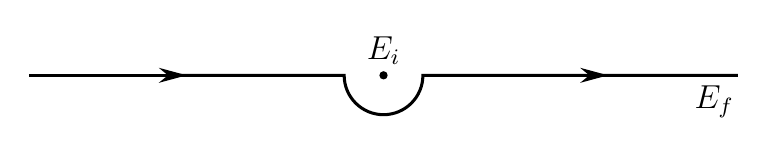
\begin{tikzpicture}[line width=1.1pt, baseline]
\draw (-4.5, 0) [-{Stealth[length=10pt, angle'=30]}]-- (-2.5, 0);
\draw (-2.7, 0) -- (-0.5, 0) 
arc[radius = 0.5cm, start angle = 180, delta angle = 180]
-- (0.5, 0) -- (2.7, 0)
(2.5, 0) [{Stealth[length=10pt, angle'=30, reversed]}-]-- (4.5, 0);
\node[font=\large,above] at (0, 0) {$E_i$};
\node[font=\large,below] at (4.2, 0) {$E_f$};
\fill (0, 0) circle(1.5pt);
\end{tikzpicture}
\end{equation}



The time factor in \eqref{43.3} shows that this function belongs, as it should, to the same energy $ E_i $ as the original unperturbed function. In other words, the function
\begin{equation}\label{43.5}
\psi_i=\psi_i^{(0)}+\int\frac{V_{fi}}{E_i-E_f+\i0}\psi_f^{(0)}\d\nu_f
\end{equation}
satisfies Schr\"odinger’s equation
\[ (\hat{H}_0+\hat{V})\psi_i=E_i\psi_i \]
It is therefore natural that the expression obtained should correspond exactly to \eqref{38.8}.\footnote{With this formula, the way in which the integral is to be taken can be found from the condition that the asymptotic expression for $ \psi_i $ at large distances should contain only an outgoing (and not an ingoing) wave (see \S136).}

The calculations given above correspond to the first approximation of perturbation theory. It is not difficult to calculate the second approximation as well. To do this, we must derive the formula for the next approximation to $ \Psi_i $; this is easily effected by using the method of \S\ref{Perturbations independent of time} (now that we know the method of dealing with the “divergent” integrals). A simple calculation gives the formula
\[ \Psi_i=\left\{\psi_i^{(0)}+\int\left[V_{fi}+\int\frac{V_{f\nu}V_{\nu i}}{E_i-E_f+\i0}\d\nu \right]\frac{\psi_f^{(0)}\d\nu_f}{E_i-E_f+\i0}  \right\}\exp\left(-\frac{\i}{\h}E_i t \right). \]



Comparing this expression with formula \eqref{43.3}, we can write down the corresponding formula for the probability (or, more precisely, the number) of transitions, by direct analogy with \eqref{43.1}:
\begin{equation}\label{43.6}
\d w_{fi}=\frac{2\pi}{\h}\left|V_{fi}+\int\frac{V_{f\nu}V_{\nu i}}{E_i-E_\nu+\i0} \right|^2\delta(E_i-E_f)\d\nu_f.
\end{equation}



It may happen that the matrix element $ V_{fi} $ for the transition considered vanishes. The effect is then zero in the first approximation, and \eqref{43.6} becomes
\begin{equation}\label{43.7}
\d w_{fi}=\frac{2\pi}{\h}\left|\int\frac{V_{f\nu}V_{\nu i}}{E_i-E_\nu}\d\nu \right|^2\delta(E_f-E_i)\d\nu_f,
\end{equation}
In applications of this formula, the point $ E_\nu = E_i $ is not usually a pole of the integrand; the manner of integrating with respect to $ E_\nu $ is then unimportant, and the integral can be taken along the real axis.

The states $\nu$ for which $ V_{f\nu} $ and $ V_{\nu i} $ are not zero are usually called \textit{intermediate states} for the transition $ i \to f $. Intuitively, we may say that this transition takes place as if in two steps $ i \to \nu $ and $ \nu\to  f $ (but such a description must not be taken literally, of course). It may happen that the transition $ i \to f $ can take place not through one but only through several successive intermediate states. Formula \eqref{43.7} can be at once generalized to such cases. For example, if two intermediate states are needed, we have
\begin{equation}\label{43.8}
\d w_{fi}=\frac{2\pi}{\h}\left|\int\frac{V_{f\nu'}V_{\nu'\nu}V_{\nu i}}{(E_i-E_{\nu'})(E_i-E_\nu)}\d\nu\d\nu'\right|^2\delta(E_f-E_i)\d\nu_f.
\end{equation}



Lastly, to clarify the mathematical significance of the integrals taken along a path of the form \eqref{43.4}, we shall prove the formula
\begin{equation}\label{43.9}
\int\frac{f(x)\d x}{x-a-\i0}=P\int\frac{f(x)\d x}{x-a}+\i\pi f(a),
\end{equation}
where the integration is along a segment of the real axis including the point $ x = a $. If we pass round the pole $ x = a $ along a semicircle of radius $\rho$, we find that the whole integral is equal to the sum of the integrals along the real axis from the lower limit to $ a -\rho  $ and from $ a +\rho $ to the upper limit, together with $ \i\pi $ times the residue of the integrand at the pole. In the limit $ \rho \to 0 $, the integrals along the real axis make the integral along the complete segment, taken as a principal value (denoted by $ P $), and the result is \eqref{43.9}, which may also be symbolically written
\begin{equation}\label{43.10}
\frac{1}{x-a-\i0}=P\frac{1}{x-a}+\i\pi\delta(x-a);
\end{equation}
$ P $ here denotes the taking of the principal value when integrating the function $ f (x)/(x - a) $.

\section{The uncertainty relation for energy}\label{The uncertainty relation for energy}
Let us consider a system composed of two weakly interacting parts. We suppose that it is known that at some instant these parts have definite values of the energy, which we denote by $ E $ and $ \epsilon $ respectively. Let the energy be measured again after some time interval $ \Delta t $; the values $ E' $, $ \epsilon' $ obtained are in general different from $ E $, $ \epsilon $. It is easy to determine the order of magnitude of the most probable value of the difference $ E'+\epsilon'-E-\epsilon $ which is found as a result of the measurement.

According to formula \eqref{42.3} with $ \omega = 0 $, the probability of a transition of the system (after time $ t $), under the action of a time-independent perturbation, from a state with energy $ E $ to one with energy $ E' $ is proportional to
\[ \left(\sin^2\frac{E'-E}{2\h}t \right)/(E'-E)2. \]
Hence we see that the most probable value of the difference $ E'- E $ is of the order of $ \h/t $.

Applying this result to the case we are considering (the perturbation being the interaction between the parts of the system), we obtain the relation
\begin{equation}\label{44.1}
|E_\epsilon-E'-\epsilon'|\Delta t\sim\h.
\end{equation}



Thus the smaller the time interval $ \Delta t $, the greater the energy change that is observed. It is important to notice that its order of magnitude $ \h/\Delta t $ is independent of the amount of the perturbation. The energy change determined by the relation \eqref{44.1} will be observed, however weak the interaction between the two parts of the system. This result is peculiar to quantum theory and has a deep physical significance. It shows that, in quantum mechanics, the law of conservation of energy can be verified by means of two measurements only to an accuracy of the order of $ \h/\Delta t $, where $ \Delta t $ is the time interval between the measurements.

The relation \eqref{44.1} is often called the uncertainty relation for energy. However, it must be emphasized that its significance is entirely different from that of the uncertainty relation $ \Delta p\Delta x \sim \h $ for the coordinate and momentum. In the latter, $ \Delta p $ and $ \Delta x $ are the uncertainties in the values of the momentum and coordinate at the same instant; they show that these two quantities can never have entirely definite values simultaneously. The energies $ E $, $ \epsilon $, on the other hand, can be measured to any degree of accuracy at any instant. The quantity $ (E + \epsilon) - (E' + \epsilon') $ in \eqref{44.1} is the difference between two exactly measured values of the energy $ E + \epsilon $ at two different instants, and not the uncertainty in the value of the energy at a given instant.

If we regard $ E $ as the energy of some system and $ \epsilon $ as that of a “measuring apparatus”, we can say that the energy of interaction between them can be taken into account only to within $ \h/\Delta t $. Let us denote by $ \Delta E ,  \Delta \epsilon,\dots $ the errors in the measurements of the corresponding quantities. In the favourable case when $ \epsilon, \epsilon' $ are known exactly ($ \Delta\epsilon =\Delta\epsilon' = 0 $), we have
\begin{equation}\label{44.2}
\Delta(E-E')\sim\frac{\h}{\Delta t}.
\end{equation}



From this relation we can derive important consequences concerning the measurement of momentum. The process of measuring the momentum of a particle (for definiteness, we shall speak of an electron) consists in a collision of the electron with some other (“measuring”) particle, whose momenta before and after the collision can be regarded as known exactly.\footnote{In the present analysis it is of no importance how the energy of the “measuring” particle is ascertained.} If we apply to this collision the law of conservation of momentum, we obtain three equations (the three components of a single vector equation) in six unknowns (the components of the momentum of the electron before and after the collision). The number of equations can be increased by bringing about a series of further collisions between the electron and “measuring” particles, and applying to each collision the law of conservation of momentum. This, however, increases the number of unknowns also (the momenta of the electron between collisions), and it is easy to see that, whatever the number of collisions, the number of unknowns will always be three more than the number of equations. Hence, in order to measure the momentum of the electron, it is necessary to bring in the law of conservation of energy at each collision, as well as that of momentum. The former, however, can be applied, as we have seen, only to an accuracy of the order of $ \h/\Delta t $, where $ \Delta t $ is the time between the beginning and end of the process in question.

To simplify the subsequent discussion, it is convenient to consider an imaginary idealized experiment in which the “measuring particle” is a perfectly reflecting plane mirror; only one momentum component is then of importance, namely that perpendicular to the plane of the mirror. To determine the momentum $ P $ of the particle, the laws of conservation of momentum and energy give the equations
\begin{equation}\label{44.3}
p'+P'-p-P'=0,
\end{equation}
\begin{equation}\label{44.4}
|\epsilon'+E'-\epsilon-E|\sim\frac{\h}{\Delta t}
\end{equation}
where $ P, E $ are the momentum and energy of the particle, and $ p, \epsilon $ those of the mirror; the unprimed and primed quantities refer to the instants before and after the collision respectively. The quantities $ p, p', \epsilon, \epsilon' $ relating to the “measuring particle” can be regarded as known exactly, i.e. the errors in them are zero. Then we have for the errors in the remaining quantities, from the above equations:
\[ \Delta P=\Delta P',\quad |\Delta E'-\Delta E|\sim\frac{\h}{\Delta t}. \]
But 
\[ \Delta E = (\p E/\p P)\Delta P = v\Delta P, \] 
where $ v $ is the velocity of the electron (before the collision), and similarly 
\[ \Delta E' = v'\Delta P' = v'\Delta P. \]
Hence we obtain
\begin{equation}\label{44.5}
|(v_x'-v_x)\delta P_x|\sim\frac{\h}{\delta t}.
\end{equation}
We have here added the suffix $ x $ to the velocity and momentum, in order to emphasize that this relation holds for each of their components separately.

This is the required relation. It shows that the measurement of the momentum of the electron (with a given degree of accuracy $ \Delta P $) necessarily involves a change in its velocity (i.e. in the momentum itself). This change becomes greater as the duration of the measuring process becomes shorter. The change in velocity can be made arbitrarily small only as $ \Delta t \to \infty $, but measurements of momentum occupying a long time can be significant only for a free particle. The non-repeatability of a measurement of momentum after short intervals of time, and the “two-faced” nature of measurement in quantum mechanics—the necessity of a distinction between the measured value of a quantity and the value resulting from the process of measurement—are here exhibited with particular clarity.\footnote{The relation \eqref{44.5} and the elucidation of the physical significance of the uncertainty relation for energy are due to N. Bohr (1928).}

The conclusion reached at the beginning of this section, which was based on perturbation theory, can also be derived from another standpoint by considering the decay of a system under the action of some perturbation. Let $ E_0 $ be some energy level of the system, calculated without any allowance for the possibility of its decay. We denote by $\tau$ the $ lifetime $ of this state of the system, i.e. the reciprocal of the probability of decay per unit time. Then we find by the same method that
\begin{equation}\label{44.6}
|E_0-E-\epsilon|\sim\h/\tau
\end{equation}
where $ E, \epsilon $ are the energies of the two parts into which the system decays. The sum $ E+\epsilon $, however, gives us an estimate of the energy of the system before it decays. Hence the above relation shows that the energy of a system, in some “quasi-stationary” state, which is free to decay can be determined only to within a quantity of the order of $ \h/\tau $. This quantity is usually called the \textit{width} $\Gamma$ of the level. Thus
\begin{equation}\label{44.7}
\Gamma\sim\h/\tau
\end{equation}

\section{Potential energy as a perturbation}\label{Potential energy as a perturbation}
The case where the total potential energy of the particle in an external field can be regarded as a perturbation merits special consideration. The unperturbed Schrödinger’s equation is then the equation of free motion of the particle:
\begin{equation}\label{45.1}
\Delta \psi^{(0)}+k^2\psi^{(0)}=0,\quad k=\frac{\sqrt{2mE}}{\h}=\frac{p}{\h}
\end{equation}
and has solutions which represent plane waves. The energy spectrum of free motion is continuous, so that we are concerned with an unusual case of perturbation theory in a continuous spectrum. The solution of the problem is here more conveniently obtained directly, without having recourse to general formulae.

The equation for the correction $ \psi^{(1)} $ to the wave function in the first approximation is
\begin{equation}\label{45.2}
\Delta\psi^{(1)}+k^2\psi^{(1)}=\frac{2mU}{\h^2}\psi^{(0)}
\end{equation}
where $ U $ is the potential energy. The solution of this equation, as we know from electrodynamics, can be written in the form of \textit{retarded potentials}, i.e. in the form\footnote{This is a particular integral of equation \eqref{45.2}, to which we may add any solution of the same equation with zero on the right-hand side, i.e. the unperturbed equation \eqref{45.1}.
}
\begin{equation}\label{45.3}
\psi^{(1)}=-\frac{m}{2\pi\h^2}\int\psi^{(0)}U(x',y',z')\e^{\i kr}\frac{\d V'}{r},
\end{equation}
where
\[ \d V'=\d x'\d y'\d z',\quad r^2=(x-x')^2+(y-y')^2+(z-z')^2. \]



Let us find what conditions must be satisfied by the field $ U $ in order that it may be regarded as a perturbation. The condition of applicability of perturbation theory is contained in the requirement that $ \psi^{(1)}\ll \psi^{(0)} $. Let $ a $ be the order of magnitude of the dimensions of the region of space in which the field is noticeably different from zero. We shall first suppose that the energy of the particle is so small that $ ka $ is at most of the order of unity. Then the factor $ \e^{\i kr} $ in the integrand of \eqref{45.3} is unimportant in an order-of-magnitude estimate, and the integral is of the order of $ \psi^{(0)}|U|a^2 $, so that
\[ \psi^{(1)}\sim(ma^2|U|\h^2)\psi^{(0)} \]
and we have the condition
\begin{equation}\label{45.4}
|U|\ll\frac{\h^2}{ma^2}\qquad(\mathrm{for}\quad ka\lesssim1).
\end{equation}
We notice that the expression on the right has a simple physical meaning; it is the order of magnitude of the kinetic energy which the particle would have if enclosed in a volume of linear dimensions $ a $ (since, by the uncertainty relation, its momentum would be of the order of $ \h/a $).

Let us consider, in particular, a potential well so shallow that the condition \eqref{45.4} holds for it. It is easy to see that in such a well there are no negative energy levels (R. Peierls 1929); this has been shown, for the particular case of a spherically symmetric well, in \S\ref{Spherical waves}, Problem, For, when $ E = 0 $, the unperturbed wave function reduces to a constant, which can be arbitrarily taken as unity: $ \psi^{(0)} = 1 $. Since $ \psi^{(1)}\ll \psi^{(0)} $, it is clear that the wave function $ \psi = 1+\psi^{(1)} $ for motion in the well nowhere vanishes; the eigenfunction, being without nodes, belongs to the normal state, so that $ E = 0 $ remains the least possible value of the energy of the particle. Thus, if the well is sufficiently shallow, only an infinite motion of the particle is possible: the particle cannot be “captured” by the well. Note that this result is peculiar to quantum theory; in classical mechanics a particle can execute a finite motion in any potential well.

It must be emphasized that all that has been said refers only to a three-dimensional well. In a one- or two-dimensional well (i.e. one in which the field is a function of only one or two coordinates), there are always negative energy levels (see the Problems at the end of this section). This is related to the fact that, in the one- and two-dimensional cases, the perturbation theory under consideration is inapplicable for an energy $ E $ which is zero (or very small).\footnote{In the two-dimensional case $ \psi^{(1)} $ is expressed (as is known from the theory of the two-dimensional wave equation) as an integral similar to \eqref{45.3}, in which, instead of $ \frac{\e^{\i kr}}{r}\d x'\d y'\d z' $ we have $ \i\pi H_0^{(1)} (kr) \d x'\d y' $, where $ H_0^{(1)} $ is the Hankel function and $ r =\sqrt{(x - x)^2 + (y - y)^2}  $. As $ k →\to0 $, the Hankel function, and therefore the whole integral, tend logarithmically to infinity.
	

Similarly, in the one-dimensional case, we have, in the integrand, $ 2\pi\i\frac{\e^{\i kr}}{k}\d x'$, where $ r = |x -x'| $, and as $ k \to0 $ $ \psi^{(1)} $ tends to infinity as $ 1/k $.}

For large energies, when $ ka\gg 1 $, the factor $ \e^{\i kr} $ in the integrand plays an important part, and markedly reduces the value of the integral. The solution \eqref{45.3} in this case can be transformed; the alternative form, however, is more conveniently derived by returning to equation \eqref{45.2}. We take as $ x $-axis the direction of the unperturbed motion; the unperturbed wave function then has the form $ \psi^{(0)} = \e^{\i kx} $ (the constant factor is arbitrarily taken as unity). Let us seek a solution of the equation
\[ \Delta \psi^{(1)}+k^2\psi^{(1)}=\frac{2m}{\h^2}U\e^{\i kx} \]
in the form $ \psi^{(1)} = \e^{\i kx}f $; in view of the assumed large value of $ k $, it is sufficient to retain in $ \Delta \psi^{(1)} $ only those terms in which the factor $ \e^{\i kx} $ is differentiated one or more times. We then obtain for $ f $ the equation
\[ 2\i k\frac{\p f}{\p x}=\frac{2mU}{\h^2}, \]
whence
\begin{equation}\label{45.5}
\psi^{(1)}=\e^{\i kx}f=-\frac{\i m}{\h^2 k}\e^{\i kx}\int U\d x.
\end{equation}



An estimation of this integral gives $ |\psi^{(1)}| \sim m|U|a/\h^2k $, so that the condition of applicability of perturbation theory in this case is
\begin{equation}\label{45.6}
|U|\ll\frac{\h^2}{ma^2}ka=\frac{\h\nu}{a},\quad ka\gg1.
\end{equation}
where $ v = k\h/m $ is the velocity of the particle. It is to be observed that this condition is weaker than \eqref{45.4}. Hence, if the field can be regarded as a perturbation at small energies of the particle, it can always be so regarded at large energies, whereas the converse is not necessarily true.\footnote{In the one-dimensional case the condition for perturbation theory to be applicable is given by the inequality \eqref{45.6} for all $ ka $. The derivation of the condition \eqref{45.4} given above for the three-dimensional case is not valid in the one-dimensional case, owing to the divergence of the resulting function $ \psi^{(1)} $ (see the preceding footnote).
}

The applicability of the perturbation theory developed here to a Coulomb field requires special consideration. In a field where $ U = \alpha/r $, it is impossible to separate a finite region of space outside which $ U $ is considerably less than inside it. The required condition can be obtained by writing in \eqref{45.6} a variable distance $ r $ instead of the parameter $ a $; this leads to the inequality
\begin{equation}\label{45.7}
\frac{\alpha}{\h v}\ll1.
\end{equation}
Thus, for large energies of the particle, a Coulomb field can be regarded as a perturbation.\footnote{It must be borne in mind that the integral \eqref{45.5} with a field $ U = \alpha/r $ diverges (logarithmically) when $ x/\sqrt{y^2 + z^2} $ is large. Hence the wave function in a Coulomb field, obtained by means of perturbation theory, is inapplicable within a narrow cone about the $ x $-axis.}

Finally, we shall derive a formula which approximately determines the wave function of a particle whose energy $ E $ everywhere considerably exceeds the potential energy $ U $ (no other conditions being imposed). In the first approximation, the wave function depends on the coordinates in the same way as for free motion (whose direction is taken as the $ x $-axis). Accordingly, let us look for $\psi$ in the form $ \psi= \e^{\i kx}F $, where $ F $ is a function of the co-ordinates which varies slowly in comparison with the factor $ \e^{\i kx} $ (but we cannot in general say that it is close to unity). Substituting in Schr\"odinger’s equation, we obtain for $ F $ the equation
\begin{equation}\label{45.8}
2\i k\frac{\p F}{\p x}=\frac{2m}{\h^2}UF,
\end{equation}
whence
\begin{equation}\label{45.9}
\psi=\e^{\i kx}F=\mathrm{const}\cdot\e^{\i kx}\exp\left(-\frac{\i}{\h v}\int U\d x \right).
\end{equation}



This is the required expression. It should, however, be borne in mind that this formula is not valid at large distances. In equation \eqref{45.8} a term $ \Delta F $ has been omitted which contains second derivatives of $ F $. The derivative $ \p^2F/{\p x}^2 $, together with the first derivative $ \p F/\p x $, tends to zero at large distances, but the derivatives with respect to the transverse coordinates $ y $ and $ z $ do not tend to zero, and can be neglected only if $ x\ll ka^2 $.





{\small
\textbf{PROBLEMS}


\textbf{1.} Determine the energy level in a one-dimensional potential well whose depth is small. It is assumed that the condition \eqref{45.4} is satisfied.





SOLUTION. We make the hypothesis, which will be confirmed by the result, that the energy level $ |E|\ll |U| $. Then, on the right-hand side of Schr\"odinger’s equation
\[ \frac{\d^2\psi}{{\d x}^2}=\frac{2m}{\h^2}(U(x)-E)\psi \]
we can neglect $ E $ in the region of the well, and regard $\psi$ as a constant, which without loss of generality can be taken as unity:
\[ \frac{\d^2\psi}{{\d x}^2}=\frac{2m}{\h^2}U. \]
We integrate this equation with respect to $ x $ between two points $ \pm x_1 $ such that $ a\ll x_1\ll 1/\varkappa $, where a is the width of the well and $ \varkappa = \sqrt{2m|E|}/\h $. Since the integral of $ U (x) $ converges, the integration on the right can be extended to the whole range from $ -\infty $ to $ +\infty $:
\begin{equation}\label{45-1-1}
\left.\frac{\d \psi}{\d x}\right|_{-x_1}^{x_1}=\frac{2m}{\h^2}\int_{-\infty}^{+\infty}U\d x.\tag{1}
\end{equation}
At large distances from the well, the wave function is of the form $ \psi = \e^{\pm\varkappa x} $. Substituting this in \eqref{45-1-1}, we find
\[ -2\varkappa=\frac{2m}{\h^2}\int_{-\infty}^{+\infty}U\d x \]
or
\[ |E|=\frac{m}{2\h^2}\left(\int_{-\infty}^{+\infty}U\d x \right)^2. \]
We see that, in accordance with the hypothesis, the energy of the level is a small quantity of a higher order (the second) than the depth of the well.





\textbf{2.} Determine the energy level in a two-dimensional potential well $ U (r) $ (where $ r $ is the polar coordinate in the plane) of small depth; it is assumed that the integral $ \int_{0}^{\infty}rU\d r $ converges.





SOLUTION. Proceeding as in the previous problem, we have in the region of the well the equation
\[ \frac{1}{r}\frac{\d}{\d r}\left(r\frac{\d\psi}{\d r} \right)=\frac{2m}{\h^2}U. \]



Integrating this with respect to $ r $ from $ 0 $ to $ r_1 $ (where $ a\ll r_1\ll 1/\varkappa $), we find
\begin{equation}\label{45-2-1}
\left.\frac{\d\psi}{\d r}\right|_{r=r_1}=\frac{2m}{\h^2 r_1}\int_{0}^{\infty}rU(r)\d r.\tag{1}
\end{equation}
At large distances from the well, the equation of free motion in two dimensions is
\[ \frac{1}{r}\frac{\d}{\d r}\left(r\frac{\d\psi}{\d r} \right)+\frac{2m}{\h^2}E\psi=0 \]
and has a solution (vanishing at infinity) $ \psi =\mathrm{const}\cdot H_0^{(1)}(\i\varkappa r) $; for small values of the argument, the leading term in this function is proportional to $ \log \varkappa r $. Bearing this in mind, we equate the logarithmic derivatives of $ \psi $ for $ r \sim a $ inside the well (the right-hand side of \eqref{45-2-1} and outside it, obtaining
\[ \frac{1}{a\log\varkappa a}\approx\frac{2m}{\h^2 a}\int_0^\infty U(r)r\d r, \]
whence
\[ |E|\sim\frac{\h^2}{ma^2}\exp\left[-\frac{\h^2}{m}\left|\int_0^\infty Ur\d r \right|^{-1} \right]. \]
We see that the energy of the level is exponentially small compared with the depth of the well.}

\chapter{THE QUASI-CLASSICAL CASE}\label{THE QUASI-CLASSICAL CASE}
\section{The wave function in the quasi-classical case}\label{The wave function in the quasi-classical case}
\section{Boundary conditions in the quasi-classical case}\label{Boundary conditions in the quasi-classical case}
\section{Bohr and Sommerfeld’s quantization rule}\label{Bohr and Sommerfeld’s quantization rule}
\section{Quasi-classical motion in a centrally symmetric field}\label{Quasi-classical motion in a centrally symmetric field}
\section{Penetration through a potential barrier}\label{Penetration through a potential barrier}
\section{Calculation of the quasi-classical matrix elements}\label{Calculation of the quasi-classical matrix elements}
\section{The transition probability in the quasi-classical case}\label{The transition probability in the quasi-classical case}
\section{Transitions under the action of adiabatic perturbations}\label{Transitions under the action of adiabatic perturbations}
\chapter{SPIN}\label{SPIN}
\section{Spin}\label{Spin}
IN BOTH classical and quantum mechanics, the law of conservation of angular momentum is a consequence of the isotropy of space with respect to a closed system. This already demonstrates the relation between the angular momentum and the symmetry properties under rotation. In quantum mechanics, however, the relation in question is a particularly far-reaching one, and essentially constitutes the basic content of the concept of angular momentum, especially as the classical definition of the angular momentum of a particle as the product $ \bm{r}\times\bm{p} $ has no direct significance in quantum mechanics, owing to the fact that position and momentum cannot be simultaneously measured.

We have seen in \S\ref{Eigenfunctions of the angular momentum} that, if the values of $ l $ and $ m $ are specified, the angular dependence of the wave function of the particle is determined, and therefore so are all its symmetry properties under rotation. The most general formulation of these properties involves specifying the transformation of the wave functions when the coordinate system is rotated.

The wave function $\psi_{LM}$ of a system of particles (with specified values of the angular momentum $ L $ and its component $ M $) remains unchanged\footnote{Apart from an unimportant phase factor.
} only in a rotation of the coordinate system about the $ z $-axis. Any rotation that alters the direction of this axis has the result that the $ z $-component of the angular momentum does not have a definite value. This means that, in the new coordinates, the wave function in general becomes a superposition (a linear combination) of $ 2L + 1 $ functions corresponding to the different possible values of $ M $ for the given $ L $. We can say that the $ 2L + 1 $ functions $\psi_{LM}$ are transformed into linear combinations of one another when the coordinate system is rotated.\footnote{In mathematical terms, these functions are the irreducible representations of the rotation group. The number of functions which are transformed into linear combinations of one another is called the dimension of the representation; it is assumed that this number cannot be made smaller by taking any other linear combinations of these functions.
} The law governing this transformation (i.e. the coefficients in the superposition as functions of the angles of rotation of the coordinate axes) is entirely determined by specifying the value of $ L $. Thus the angular momentum acquires the significance of a quantum number which classifies the states of the system according to their transformation properties under rotation of the coordinate system. This aspect of the concept of angular momentum in quantum mechanics is particularly important because it is not directly related to the explicit angular dependence of the wave functions; the law of mutual transformation of these functions can be stated without reference to that dependence.

Let us consider a composite particle, such as an atomic nucleus, which is at rest as a whole and is in a definite internal state. In addition to an internal energy, it has also an angular momentum of definite magnitude $ L $, due to the motion of the particles within the nucleus. This angular momentum can have $ 2L + 1 $ different orientations in space. Thus, in considering the movement of a complex particle as a whole, we must assign to it, as well as its coordinates, another discrete variable: the projection of its internal angular momentum on some chosen direction in space.

However, with the preceding understanding of the concept of angular momentum, the origin of it becomes unimportant, and we naturally arrive at the concept of an “intrinsic” angular momentum which must be ascribed to the particle regardless of whether it is “composite” or “elementary”.

Thus, in quantum mechanics an elementary particle must be assigned a certain “intrinsic” angular momentum unconnected with its motion in space. This property of elementary particles is peculiar to quantum theory (it disappears in the limit $ \h\to 0 $), and therefore has in principle no classical interpretation.\footnote{In particular, it would be wholly meaningless to imagine the “intrinsic” angular momentum of an elementary particle as being the result of its rotation “about its own axis”.
}

The intrinsic angular momentum of a particle is called its \textit{spin}, as distinct from the angular momentum due to the motion of the particle in space, called the \textit{orbital angular momentum}.\footnote{The physical idea that an electron has an intrinsic angular momentum was put forward by G. Uhlenbeck and S. Goudsmit in 1925. Spin was introduced into quantum mechanics in 1927 by W. Pauli.
} The particle concerned may be either elementary, or composite but behaving in some respect as an elementary particle (e.g. an atomic nucleus). The spin of a particle (measured, like the orbital angular momentum, in units of $ \h $) will be denoted by $ s $.

For particles having spin, the description of the state by means of the wave function must determine the probability not only of its different positions in space but also of the possible orientations of the spin. Thus the wave function must depend not only on three continuous variables, the coordinates of the particle, but also on a discrete spin variable, which gives the value of the projection of the spin on a selected direction in space (the z-axis) and takes a limited number of discrete values, which we shall denote by $\sigma$.

Let $ \psi(x, y, z; \sigma) $ be such a wave function. It is essentially a set of several different functions of the coordinates, corresponding to different values of $\sigma$; these functions will be called the \textit{spin components} of the wave function. The integral
\[ \int|\psi(x,y,z;\sigma)|^2\d V \]
determines the probability that the particle has a certain value of $\sigma$. The probability that the particle is in the volume element $ \d V $ with any value of $\sigma$ is
\[ \d V\sum_{\sigma}|\psi(x,y,z;\sigma)|^2. \]



The quantum-mechanical spin operator, on being applied to the wave function, acts on the spin variable $\sigma$. In other words, it in some way linearly transforms the components of the wave function into one another. The form of this operator will be established later. However, it is easy to see from very general considerations that the operators $\hat{s}_x,\hat{s}_y,\hat{s}_z$ satisfy the same commutation conditions as the operators of the orbital angular momentum.

The angular momentum operator is essentially the same as that of an infinitely small rotation. In deriving, in \S\ref{Angular momentum}, the expression for the orbital angular momentum operator, we considered the result of applying the rotation operator to a function of the coordinates. In the case of the spin, this derivation becomes invalid, since the spin operator acts on the spin variable, and not on the coordinates. Hence, to obtain the required commutation relations, we must consider the operation of an infinitely small rotation in a general form, as a rotation of the system of coordinates. If we successively perform infinitely small rotations about the $ x $-axis and the $ y $-axis, and then about the same axes in the reverse order, it is easy to see by direct calculation that the difference between the results of these two operations is equivalent to an infinitely small rotation about the $ z $-axis (through an angle equal to the product of the angles of rotation about the $ x $ and $ y $-axes). We shall not pause here to carry out these simple calculations, as a result of which we again obtain the usual commutation relations between the operators of the components of angular momentum; these must therefore hold for the spin operators also:
\begin{equation}\label{54.1}
\{\hat{s}_y,\hat{s}_z\}=\i\hat{s}_x,\quad\{\hat{s}_z,\hat{s}_z\}=\i\hat{s}_y,\quad\{\hat{s}_x,\hat{s}_y\}=\i\hat{s}_z
\end{equation}
together with all the physical consequences resulting from them.

The commutation relations \eqref{54.1} enable us to determine the possible values of the absolute magnitude and components of the spin. All the results derived in \S\ref{Eigenvalues of the angular momentum} (formulae \eqref{27.7}–\eqref{27.9}) were based only on the commutation relations, and hence are fully applicable here also; we need only replace $ \bm{L} $ in these formulae by $ \bm{s} $. It follows from formula \eqref{27.7} that the eigenvalues of the component of the spin form a sequence of numbers differing by unity. However, we cannot now assert that these values must be integral, as we could for the component $ L_z $ of the orbital angular momentum (the derivation given at the beginning of \S\ref{Eigenvalues of the angular momentum} is invalid here, since it was based on the expression \eqref{26.14} for the operator $\hat{l}_z$, which holds only for the orbital angular momentum).

Moreover, we find that the sequence of eigenvalues $ s_z $ is limited above and below by values equal in absolute magnitude and opposite in sign, which we denote by $ \pm s $. The difference $ 2s $ between the greatest and least values of $ s_z $ must be an integer or zero. Consequently $ s $ can take the values $ 0, 1/2, 1, 3/2,\dots $

Thus the eigenvalues of the square of the spin are
\begin{equation}\label{54.2}
\bm{s}^2=s(s+1)
\end{equation}
where $ s $ can be either an integer (including zero) or half an integer. For given $ s $, the component $ s_z $ of the spin can take the values $ s, s - 1, \dots, -s $, i.e. $ 2s+1 $ values in all. Accordingly, the wave function of a particle with spin $ s $ has $ 2s + 1 $ components.\footnote{Since $ s $ is fixed for each kind of particle, the spin angular momentum $ \h s $ becomes zero in the limit of classical mechanics ($ \h\to0 $). This consideration does not apply to the orbital angular momentum, since $ l $ can take any value. The transition to classical mechanics is represented by $ \h $ tending to zero and $ l $ simultaneously tending to infinity, in such a way that the product $ \h l $ remains finite.}

Experiment shows that the majority of the elementary particles (electrons, positrons, protons, neutrons, $ \mu $-mesons and all hyperons ($ \Lambda,\Sigma,\Xi $)) have a spin of $ 1/2 $. There are also elementary particles, the $\pi$-mesons and the $ K $-mesons, whose spin is zero.

The total angular momentum of a particle is composed of its orbital angular momentum $ \bm{l} $ and its spin $ \bm{s} $. Their operators act on functions of different variables, and therefore, of course, commute. The eigenvalues of the total angular momentum
\begin{equation}\label{54.3}
\bm{j}=\bm{l}+\bm{s}
\end{equation}
are determined by the same “vector model” rule as the sum of the orbital angular momenta of two different particles (\S\ref{Addition of angular momenta}). That is, for given values of $ l $ and $ s $, the total angular momentum can take the values $ l+s, l+s- 1, \dots, |l−s| $. Thus, for an electron (spin $ 1/2 $) with non-zero orbital angular momentum $ l $, the total angular momentum can be $ j = l \pm1/2 $; for $ l = 0 $ the angular momentum $ j $ has, of course, only the one value $ j = 1/2$.

The operator of the total angular momentum $ \bm{J} $ of a system of particles is equal to the sum of the operators of the angular momentum $ \bm{j} $ of each particle, so that its values are again determined by the vector model rules. The angular momentum $ \bm{J} $ can be put in the form
\begin{equation}\label{54.4}
\bm{J}=\bm{L}+\bm{S},\quad\bm{L}=\sum_{a}\bm{l}_a,\quad\bm{S}=\sum_{a}\bm{s}_a,
\end{equation}
where $ \bm{S} $ may be called the total spin and $ \bm{L} $ the total orbital angular momentum of the system. We notice that, if the total spin of the system is half-integral (or integral), the same is true of the total angular momentum, since the orbital angular momentum is always integral. In particular, if the system consists of an even number of similar particles, its total spin is always integral, and therefore so is the total angular momentum.

The operators of the total angular momentum $ \bm{j} $ of a particle (or $ \bm{J} $, of a system of particles) satisfy the same commutation rules as the operators of the orbital angular momentum or the spin, since these rules are general commutation rules holding for any angular momentum. The formulae \eqref{27.13} for the matrix elements of angular momentum, which follow from the commutation rules, are also valid for any angular momentum, provided that the matrix elements are defined with respect to the eigenstates of this angular momentum. Formulae \eqref{29.7}—\eqref{29.10} for the matrix elements of arbitrary vector quantities also remain valid (with appropriate change of notation).





{\small
	
\textbf{PROBLEMS}


A particle with spin $ 1/2 $ is in a state with a definite value $ s_z = 1/2 $. Determine the probabilities of the possible values of the component of the spin along an axis $ z' $ at an angle $\theta$ to the $ z $-axis.





SOLUTION. The mean spin vector $ \bar{\bm{s}} $ is evidently along the $ z $-axis and has magnitude $ 1/2 $. Taking the component along the $ z' $-axis, we find that the mean value of the spin in that direction is $ \bar{s_{z'}}=(1/2)\cos\theta $. We also have $ \bar{s_{z'}}=(1/2)(w_++w_-) $ where $ w_\pm $ are the probabilities of the values $ s_{z'} = \pm1/2 $. Since $ w_++w_-= 1 $, we find 
\[ w_+ = \cos2\theta, w_- = \sin2\theta. \] }





\section{The spin operator}\label{The spin operator}
In the rest of this chapter we shall not be interested in the dependence of the wave functions on the coordinates. For example, in speaking of the behaviour of the functions $ \psi(x, y, z; \sigma) $ when the system of coordinates is rotated, we can suppose that the particle is at the origin, so that its coordinates remain unchanged by such a rotation, and the results obtained will characterize the behaviour of the function $ \psi $ with regard to the spin variable $ \sigma $.

The variable $\sigma$ differs from the ordinary variables (the coordinates) by being discrete. The most general form of a linear operator acting on functions of a discrete variable $\sigma$ is
\begin{equation}\label{55.1}
\left(\hat{f}\psi \right)(\sigma)=\sum_{\sigma'}f_{\sigma\sigma'}\psi(\sigma')
\end{equation}
where the $ f_{\sigma\sigma'} $, are constants. We put $\psi$  in parentheses in order to emphasize that the spin argument following it is not that of the original function $\psi$ but that of the function resulting from it under the action of the operator $ \hat{f} $. It is easy to see that the quantities $ f_{\sigma\sigma'} $, are the same as the matrix elements of the operator, defined by the usual rule \eqref{11.5}.\footnote{Note that the suffixes in the matrix elements on the right of \eqref{55.1} are written in an order which is, in a sense, the reverse of the usual order in \eqref{11.11}.
}

The integration over the coordinates in \eqref{11.5} is here replaced by summation over the discrete variable, so that the definition of the matrix element is
\begin{equation}\label{55.2}
f_{\sigma_2\sigma_1}=\sum_{\sigma}\psi^*_{\sigma_2}(\sigma)\left[\hat{f}\psi_{\sigma_1}(\sigma) \right]
\end{equation}
Here $ \psi_{\sigma_1}(\sigma) $ and $ \psi_{\sigma_2}(\sigma) $ are the eigenfunctions of the operator $ \hat{s}_z $ corresponding to the eigenvalues $ s_z = \sigma_1 $ and $ \sigma_2 $; each such function corresponds to a state in which the particle has a definite value of $ s_z $, i.e. in which only one component of the wave function is non-zero:\footnote{More precisely, we should write
\[ \psi_{\sigma_1}(\sigma)=\psi(x,y,z)\delta_{\sigma_1\sigma}; \]	
in \eqref{55.3} the coordinate factors are omitted, being unimportant in this connection.
	
We must once again emphasize the distinction between the specified eigenvalue $ \sigma_1 $ or $ \sigma_2 $ of $ s_z $ and the independent variable $\sigma$.
}
\begin{equation}\label{55.3}
\psi_{\sigma_1}(\sigma)=\delta_{\sigma\sigma_1},\quad\psi_{\sigma_2}(\sigma)=\delta_{\sigma\sigma_2}.
\end{equation}
According to \eqref{55.1},
\[ \left(\hat{f}\psi \right)(\sigma)=\sum_{\sigma'}f_{\sigma\sigma'}\psi_{\sigma_1}(\sigma')=\sum_{\sigma'}f_{\sigma\sigma'}\delta_{\sigma'\sigma_1}=f_{\sigma\sigma'} \]
and on substitution of this and $ \psi_{\sigma_2}(\sigma) $ the equation \eqref{55.2} is satisfied identically; this completes the proof.

Thus the operators acting on functions of $\sigma$ can be represented in the form of $ (2s + 1) $-rowed matrices. In particular, we have for the operator of the spin itself, acting on the wave function, by \eqref{55.1},
\begin{equation}\label{55.4}
\left(\hat{\bm{s}}\psi \right)(\sigma)=\sum_{\sigma'}\bm{s}_{\sigma\sigma'}\psi(\sigma')
\end{equation}
According to what has been said at the end of \S\ref{Spin}, the matrices $ \hat{s}_x, \hat{s}_y, \hat{s}_z $ are identical with the matrices $ \hat{L}_x, \hat{L}_y, \hat{L}_z $ obtained in \S\ref{Eigenvalues of the angular momentum}, where the letters $ L $ and $ M $ need only be replaced by $ s $ and $\sigma$:
\begin{equation}\label{55.5}
\begin{split}
(s_x)_{\sigma,\sigma-1}=(s_x)_{\sigma-1,\sigma}&=\frac{1}{2}\sqrt{(s+\sigma)(s-\sigma+1)},\\
(s_y)_{\sigma,\sigma-1}=-(s_y)_{\sigma-1,\sigma}&=-\frac{\i}{2}\sqrt{(s+\sigma)(s-\sigma+1)},\\
(s_z)_{\sigma\sigma}&=\sigma.
\end{split}
\end{equation}
This determines the spin operator.

In the important case of a spin of $ 1/2 $ ($ s = 1/2, σ = \pm1/2 $), these matrices have two rows, and are of the form
\begin{equation}\label{55.6}
\hat{\bm{s}}=\frac{1}{2}\hat{\bm{\sigma}}
\end{equation}
where\footnote{In the tabular matrices \eqref{55.7} the rows and columns are numbered by the values of σ, the row number corresponding to the first and the column number to the second suffix of the matrix element. In the present case, these numbers are $ +1/2 $ and $ -1/2 $. The action of the. operator shown by \eqref{55.4} multiplies row $\sigma$ of the matrix by a column matrix containing the components of the wave function:
	\[ \psi=\left(\begin{array}{c}
	\psi(1/2)\\
	\psi(-1/2)
	\end{array}\right) \]
}
\begin{equation}\label{55.7}
\hat{\bm{\sigma}}_x=\left(\begin{array}{cc}
0&1\\
1&0
\end{array} \right),\quad\hat{\bm{\sigma}}_y=\left( \begin{array}{cc}
0&-\i\\\i&0
\end{array}\right),\quad
\hat{\bm{\sigma}}_z=\left(\begin{array}{cc}
1&0\\
0&-1
\end{array} \right).
\end{equation}


These are called \textit{Pauli matrices}. The matrix $ \hat{\bm{s}}_z=\frac{\hat{\bm{\sigma}}_z}{2} $ is diagonal, as it should be, since it is defined in terms of the eigenfunctions of the quantity $ \bm{s}_z $ itself.\footnote{There should be no misunderstanding because of the use of the same letter to denote the spin component and the Pauli matrices, since the latter always have the circumflex.
}

The following are some specific properties of the Pauli matrices. Direct multiplication of the matrices \eqref{55.7} gives the equations
\begin{equation}\label{55.8}
\begin{split}
\hat{\bm{\sigma}}_x^2=\hat{\bm{\sigma}}_y^2&=\hat{\bm{\sigma}}_z^2=1\\
\hat{\bm{\sigma}}_y\hat{\bm{\sigma}}_z=\i\hat{\bm{\sigma}}_x,\quad\hat{\bm{\sigma}}_z\hat{\bm{\sigma}}_x&=\i\hat{\bm{\sigma}}_y,\quad\hat{\bm{\sigma}}_x\hat{\bm{\sigma}}_y=\i\hat{\bm{\sigma}}_z
\end{split}
\end{equation}
Combining these with the general commutation rules \eqref{54.1}, we find that
\begin{equation}\label{55.9}
\hat{\bm{\sigma}}_\i\hat{\bm{\sigma}}_k+\hat{\bm{\sigma}}_k\hat{\bm{\sigma}}_\i=2\delta_{\i k}
\end{equation}
i.e. the Pauli matrices anticommute with one another. By means of these equations, we can easily verify the following useful formulae:
\begin{equation}\label{55.10}
\hat{\bm{\sigma}}^2=3,\quad (\hat{\bm{\sigma}}\cdot\bm{a})(\hat{\bm{\sigma}}\cdot\bm{b})=\bm{a}\cdot\bm{b}+\i\hat{\bm{\sigma}}\cdot\bm{a}\times\bm{b}.
\end{equation}
where $ \bm{a} $ and $ \bm{b} $ are any vectors.\footnote{The terms on the right of \eqref{55.8}–\eqref{55.10} which are independent of $\hat{\bm{\sigma}}$ must, of course, be understood as constants multiplying the unit two-by-two matrix.
} According to these relations, any scalar polynomial formed from the matrices $ \hat{\bm{\sigma}}_i $ can be reduced to terms independent of $ \hat{\bm{\sigma}} $ and terms linear in $ \hat{\bm{\sigma}} $; hence it follows that any scalar function of the operator ∂ reduces to a linear function (see Problem 1). Lastly, the values of the traces (sums of diagonal elements) of the Pauli matrices and their products are
\begin{equation}\label{55.11}
\mathrm{tr}\hat{\sigma}_i=0,\quad\mathrm{tr}\hat{\sigma}_i\hat{\sigma}_k=2\delta_{ik}.
\end{equation}


Subsequent sections of this chapter give a more detailed account of the spin properties of wave functions, including their behaviour under any rotation of the coordinate system, but we may note immediately an important property of these functions, namely their behaviour in respect of rotations about the $ z $-axis.

Let there be an infinitesimal rotation through an angle $ \delta\phi $ about the $ z $-axis. The operator of such a rotation is expressed in terms of the angular momentum operator (in this case, the spin operator) as $ 1 + \i \delta\phi\cdot\hat{s}_z $. As a result of the rotation, the functions $ \psi(\sigma) $ therefore become $ \psi(\sigma) + \delta\psi(\sigma) $, where
\[ \delta\psi(\sigma)=\i\delta\phi\cdot\hat{s}_z\psi(\sigma)=\i\sigma\psi(\sigma)\delta\phi \]



Writing this relation in the form $ \d\psi/\d\phi = \i\sigma\psi(\sigma) $ and integrating, we find that a rotation through a finite angle $\phi$ changes the functions $\psi(\sigma)$ into
\begin{equation}\label{55.12}
\psi(\sigma)'=\psi(\sigma)\e^{\i\sigma\phi}
\end{equation}
In particular, a rotation through $ 2\pi $ multiplies them by a factor $ \e^{2\pi\i\sigma} $, which is the same for all $\sigma$ and is equal to $ (-1)^{2s} $ (since $ 2\sigma $ always has the same parity as $ 2s $). Thus, in a complete rotation of the coordinate system about the $ z $-axis, the wave functions of particles with integral spin return to their original values, and those of particles with half-integral spin change sign.





{\small
\textbf{PROBLEMS}


\textbf{1.} Reduce an arbitrary function of the scalar $ a + \bm{b}\cdot\hat{\bm{\sigma}} $ linear in the Pauli matrices to another linear function.





SOLUTION. TO determine the coefficients in the required formula
\[  f (a + \bm{b}\cdot\hat{\bm{\sigma}}) = \bm{A}+\bm{B}\hat{\bm{\sigma}},  \]
we note that, when the $ z $-axis is taken in the direction of $ \bm{b} $, the eigenvalues of the operator $ a + \bm{b}\cdot\hat{\bm{\sigma}} $ are $ a \pm b $, and the corresponding eigenvalues of the operator $ f (a + \bm{b}\cdot\hat{\bm{\sigma}})  $ are $ f (a \pm b) $. Hence we find 
\[ A = \frac{1}{2}[f (a + b) + f (a − b)], \bm{B} = \frac{\bm{b}}{2b} [f (a + b)-f (a−b)]. \]





\textbf{2.} Determine the values of the scalar product $ \bm{S}_1\cdot\bm{S}_2 $ of spins ($ 1/2 $) of two particles in states in which the total spin of the system, $ \bm{S} = \bm{s}_1 + \bm{s}_2 $, has definite values ($ 0 $ or $ 1 $).





SOLUTION. From the general formula \eqref{31.3}, which is valid for the addition of any two angular momenta, we find 
\[ \bm{s}_1\cdot \bm{s}_2 = 1/4\text{ for }S = 1,\quad \bm{s}_1\cdot \bm{s}_2 = -3/4\text{ for }S = 0. \]





\textbf{3.} Which powers of the operator ŝ of an arbitrary spin $\hat{\bm{s}}$ are independent?





SOLUTION. The operator
\[ (\hat{s}_z-s)(\hat{s}_z-s+1)\dots(\hat{s}_z+s), \]
formed from the differences between $\hat{s}_z$ and all possible eigenvalues $ s_z $, gives zero when it is applied to any wave function, and is therefore itself zero. Hence it follows that $ (\hat{s}_z)^{2s+1} $ is expressed in terms of lower powers of the operator $\hat{s}_z$, so that only its powers from $ 1 $ to $ 2s $ are independent.}
\section{Spinors}\label{Spinors}
When the spin is zero, the wave function has only one component, $ \psi(0) $. The effect of the spin operator is to reduce it to zero: $ \hat{\bm{s}}\psi= 0 $. The relation between $ \hat{\bm{s}} $ and the operator of an infinitesimal rotation implies that the wave function of a particle with zero spin is invariant under rotation of the coordinate system, i.e. it is a scalar.

The wave function of a particle with spin $ 1/2 $ has two components, $ \psi(1/2) $ and $ \psi(-1/2) $. For convenience in later generalizations, we shall distinguish these components by the superscripts $ 1 $ and $ 2 $ respectively. The two-component quantity
\begin{equation}\label{56.1}
\psi=\left(\begin{array}{c}
\psi^1\\\psi^2
\end{array} \right)\equiv\left(\begin{array}{c}
\psi\left(1/2\right)\\\psi\left(-1/2\right)
\end{array} \right)
\end{equation}
is called a \textit{spinor}.

In any rotation of the coordinate system, the components of the spinor undergo a linear transformation:
\begin{equation}\label{56.2}
\psi^{1'}=a\psi^1+b\psi^2,\quad\psi^{2'}=c\psi^1+d\psi^2.
\end{equation}
This may be written
\begin{equation}\label{56.3}
\psi^{\lambda'}=(\hat{U}\psi)^\lambda,\quad\hat{U}=\begin{array}{cc}
a&b\\
c&d
\end{array}
\end{equation}
where $\hat{U}$ is the transformation matrix.\footnote{The notation $ \hat{U}\psi $ implies that the rows of the matrix $\hat{U}$ are multiplied by the column $\psi$.} Its elements are in general complex functions of the angles of rotation of the coordinate axes. They are connected by relations which follow directly from the physical conditions imposed on the spinor as the wave function of a particle.

Let us consider the bilinear form
\begin{equation}\label{56.4}
\psi^1\phi^2-\psi^2\phi^1,
\end{equation}
where $\psi$ and $\phi$ are two spinors. A simple calculation gives
\[ \psi^{1'}\phi^{2'}-\psi^{2'}\phi^{1'}=(ad-bc)(\psi^1\phi^2-\psi^2\phi^1), \]
i.e. \eqref{56.4} is transformed into itself when the coordinate system is rotated. If, however, there is only one function which is transformed into itself, it can be regarded as corresponding to zero spin, and therefore must be a scalar, i.e. must remain unchanged when the coordinate system is rotated in any manner. Hence we have
\begin{equation}\label{56.5}
ad-bc=1;
\end{equation}
the determinant of the transformation matrix is unity.\footnote{Such a transformation of two quantities is called a \textit{binary transformation}.}

Further relations follow from the requirement that the expression
\begin{equation}\label{56.6}
\psi^1\psi^{1*}+\psi^2\psi^{2*},
\end{equation}
which determines the probability of finding the particle at a given point in space, should be a scalar. A transformation which leaves unchanged the sum of the squared moduli of the quantities is a unitary transformation, i.e. we must have $ \hat{U}^\dagger=\hat{U}^{-1} $ (see \S\ref{Transformation of matrices}). With the condition \eqref{56.5} the inverse matrix is
\[ \hat{U}^{-1}=\left(\begin{array}{cc}
d&-b\\
-c&a
\end{array}\right). \]
Equating this to the Hermitian conjugate matrix
\[ \hat{U}^\dagger=\left(\begin{array}{cc}
a^*&c^*\\
b^*&d^*
\end{array}\right), \]
we find
\begin{equation}\label{56.7}
a=d^*,\quad b=-c^*
\end{equation}


By virtue of the relations \eqref{56.5} and \eqref{56.7}, the four complex quantities $ a, b, c, d $ actually contain only three independent real parameters, corresponding to the three angles which define a rotation of a three-dimensional system of coordinates.

Comparison of the expressions for the scalars \eqref{56.4} and \eqref{56.6} shows that $\psi^{1*}$ and $\psi^{2*}$ must be transformed as $\psi^2$ and $ -\psi^1 $ respectively. It is easy to verify that this is in fact so, using \eqref{56.5} and \eqref{56.7}.\footnote{This property is closely associated with symmetry under time reversal. The latter (see \S\ref{The fundamental properties of Schr\"odinger's equation}) involves the replacement of the wave function by its complex conjugate. Under time reversal, the angular momentum components also change sign. Hence the functions that are the complex conjugates of the components $ \psi^1 \equiv \psi(1/2) $ and $ \psi^2 \equiv \psi(-1/2) $ must have properties equivalent to those of the components corresponding to spin projections $ -1/2 $ and $ 1/2 $ respectively.
}

It is possible to put the algebra of spinors in a form analogous to that of tensor algebra. This is done by introducing, in addition to \textit{contravariant} spinor components $ \psi^1, \psi^2 $ (with superscripts), the \textit{covariant} components (with subscripts), defined by
\begin{equation}\label{56.8}
\psi_1=\psi^2,\quad\psi_2=-\psi^1
\end{equation}
The invariant combination \eqref{56.4} of the two spinors may also be written as a scalar product
\begin{equation}\label{56.9}
\psi^\lambda\phi_\lambda=\psi^1\phi_1+\psi^1\phi_2-\psi^2\phi_1;
\end{equation}
here and below, summation over repeated (\textit{dummy}) indices is implied, as in tensor algebra. We may note the following rule which has to be borne in mind in spinor algebra. We have
\[ \psi^\lambda\phi_\lambda=\psi^1\phi_1+\psi^2\phi_2=-\psi_2\phi^2-\psi_1\phi^1. \]
Thus
\begin{equation}\label{56.10}
\psi^\lambda\phi_\lambda=-\psi_\lambda\phi^\lambda
\end{equation}
Hence it is evident that the scalar product of any spinor with itself is zero:
\begin{equation}\label{56.11}
\psi^\lambda\psi_\lambda=0.
\end{equation}


According to the foregoing discussion, the quantities $\psi_1$ and $\psi_2$ are transformed as $ \psi^{1*} $ and $ \psi^{2*} $, i.e.
\begin{equation}\label{56.12}
\psi_\lambda'=\left(\hat{U}^*\psi \right)_\lambda
\end{equation}


The product $ \hat{U}^*\psi $ may also be written as $ \psi\tilde{\hat{U}^*} $, with the transposed matrix $\tilde{\hat{U}^*}$. Since $\hat{U}$ is unitary, we have $ \tilde{\hat{U}^*}=\hat{U}^{-1} $, so that $ \psi_\lambda'=\left(\psi\hat{U}^{-1}\right)_\lambda $ or\footnote{The notation $\psi\hat{U}$ (with $\psi$ to the left of $\hat{U}$) denotes that the components ($ \psi_1\psi_2 $) as a row are multiplied by the columns of the matrix $\hat{U}$.
}
\begin{equation}\label{56.13}
\psi_\lambda=\left(\psi'\hat{U} \right)_\lambda
\end{equation}


Analogously to the transition from vectors to tensors in ordinary tensor algebra, we can introduce the idea of spinors of higher rank. Thus, a quantity $\psi^{\lambda\mu}$, having four components which are transformed as the products $ \psi^\lambda\phi^\mu $ of the components of two spinors of rank one, is called a spinor of rank two. Besides the contra variant components $\psi^{\lambda\mu}$ we can consider the covariant components $\psi^{\lambda\mu}$ and the mixed components $ \psi^{\mu}_\lambda $ which are transformed as the products $ \psi_\lambda\phi_mu $ and $ \psi_\lambda\phi^\mu $ respectively. Spinors of any rank are similarly defined.

The transition from contravariant to covariant spinor components and \textit{vice versa} may be written
\begin{equation}\label{56.14}
\psi_\lambda=g_{\\lambd
\mu}\psi^\mu,\quad\psi^\lambda=g^{\mu\lambda}\psi_mu,
\end{equation}
where
\begin{equation}\label{56.15}
\left(g_{\lambda\mu}\right)=\left(g^{\lambda\mu}\right)=\left(\begin{array}{cc}
0&1\\-1&0
\end{array}\right)
\end{equation}
is the \textit{metric spinor} in a vector space of two dimensions. Thus we have, for example,
\[ \psi_\lambda^\mu=g_{\lambda\nu}\psi^{\nu\mu},\quad\psi_{\lambda\mu}=g_{\lambda\nu}g_{\mu\rho}\psi^{\nu\rho} \]
so that $ \psi_{12} = -\psi_1^{\text{ }1} = -\psi^{21}, \psi_{11} = \psi_1^{\text{ }2} = \psi^{22} $, and so on.

The quantities $ g_{\lambda\mu} $ themselves form an antisymmetric unit spinor of rank two. It is easy to see that the values of its components remain unchanged under transformations of the coordinates, and that
\begin{equation}\label{56.16}
g_{\lambda\nu}g^{\mu\nu}=\delta_\lambda^\mu
\end{equation}
where $ \delta_1^1 = \delta_2^2 = 1, \delta_2^1 = \delta_1^2 = 0 $.

As in ordinary tensor algebra, there are two fundamental operations in spinor algebra: multiplication, and contraction with respect to a pair of indices. The \textit{multiplication} of two spinors gives a spinor of higher rank; thus, from two spinors of ranks two and three, $\psi_{\lambda\mu}$ and $ \psi^{\nu\rho\sigma} $, we can form a spinor of rank five, $\psi_{\lambda\mu}\psi^{\nu\rho\sigma}  $. \textit{Contraction} with respect to a pair of indices (i.e. summation of the components over corresponding values of one covariant and one contravariant index) decreases the rank of a spinor by two. Thus, a contraction of the spinor $ \psi_{\lambda\mu}{}^{\nu\rho\sigma} $ with respect to the indices $\mu$ and $\nu$ gives the spinor  $\psi_{\lambda\mu}{}^{\mu\rho\sigma} $ of rank three; the contraction of the spinor $ \psi_\lambda{}^{\mu} $ gives the scalar $ \psi_\lambda{}^{\lambda} $. Here there is a rule similar to that expressed by formula \eqref{56.10}: if we interchange the upper and lower indices with respect to which the contraction is effected, the sign is changed (i.e. $ \psi_\lambda{}^{\lambda}=-\psi^\lambda{}_{\lambda} $). Hence, in particular, it follows that, if a spinor is symmetrical with respect to any two of its indices, the result of a contraction with respect to these indices is zero. Thus, for a symmetrical spinor $ \psi_{\lambda\mu} $ of rank two, we have $ \psi_\lambda{}^\lambda = 0 $.

A spinor of rank $ n $ symmetrical with respect to all its indices is called a \textit{symmetrical spinor} of rank $ n $. From an asymmetrical spinor we can construct a symmetrical one by the process of \textit{symmetrization}, i.e. summation of the components obtained by all possible interchanges of the indices. From what has been said above, it is impossible to construct (by contraction) a spinor of lower rank from the components of a symmetrical spinor.

Only a spinor of rank two can be antisymmetrical with respect to all its indices. For, since each index can take only two values, at least two out of three or more indices must have the same value, and therefore the components of the spinor are zero identically. Any antisymmetrical spinor of rank two is a scalar multiple of the unit spinor $ g_{\lambda\mu} $. We may notice here the following relation:
\begin{equation}\label{56.17}
g_{\lambda\mu}\psi_\nu+g_{\mu\nu}\psi_\lambda+g_{\nu\lambda}\psi_\mu=0
\end{equation}
(where $\psi_\lambda$ is any spinor), which follows from the above; this rule is simply a consequence of the fact that the expression on the left is (as we may easily verify) an antisymmetrical spinor of rank three.

The spinor which is the product of a spinor $\psi_{\lambda\mu}$ with itself, on contraction with respect to one pair of indices, becomes antisymmetrical with respect to the other pair:
\[ \psi_{\lambda\nu}\psi_\mu{}^\nu=-\psi_\lambda{}^\nu\psi_{\mu\nu}. \]
Hence, from what was said above, this spinor must be a scalar multiple of the spinor $ g_{\lambda\mu} $. Defining the scalar factor so that contraction with respect to the second pair of indices gives the correct result, we find
\begin{equation}\label{56.18}
\psi_{\lambda\nu}\psi_nu{}^\nu=-(1/2)\psi_{\rho\sigma}\psi^{\rho\sigma}g_{\lambda\mu}
\end{equation}


The components of the spinor $\psi_{\lambda\mu\dots}{}^*$ which is the complex conjugate of $ \psi_{\lambda\mu\dots} $ are transformed as the components of a contravariant spinor $ \phi^{\lambda\mu\dots} $, and conversely. The sum of the squared moduli of the components of any spinor is consequently invariant.

\section{The wave functions of particles with arbitrary spin}\label{The wave functions of particles with arbitrary spin}
Having developed a formal algebra for spinors of any rank, we can now turn to our immediate problem, to study the properties of wave functions of particles with arbitrary spin.

This subject is conveniently approached by considering an assembly of $ n $ particles with spin $ 1/2 $. The greatest possible value of the $ z $-component of the total spin is $ n/2 $, which is obtained when $ s_z = 1/2 $ for every particle (i.e. all the spins are directed the same way, along the $ z $-axis). In this case we can evidently say that the total spin $ S $ of the system is also $ n/2 $.

All the components of the wave function $ \psi(\sigma_1, \sigma_2, \dots, \sigma_n) $ of the system of particles are then zero, except for $ \psi(1/2, 1/2, \dots,1/2) $. If we write the wave function as a product of $ n $ spinors $ \psi^\lambda\psi^\mu\dots $, each of which refers to one of the particles, only the component with $ \lambda, \mu,\dots = 1 $ in each spinor is not zero. Thus only the product $ \psi^1\phi^1 $ is not zero. The set of all these products, however, is a spinor of rank $ n $ which is symmetrical with respect to all its indices. If we transform the coordinate system (so that the spins are not directed along the $ z $-axis), we obtain a spinor of rank $ n $, general in form except that it is symmetrical as before.

The spin properties of wave functions, being essentially their properties with respect to rotations of the coordinate system, are identical for a particle with spin $ s $ and for a system of $ n = 2s $ particles each with spin $ 1/2 $ directed so that the total spin of the system is $ s $. Hence we conclude that the wave function of a particle with spin $ s $ is a symmetrical spinor of rank $ n = 2s $.

It is easy to see that the number of independent components of a symmetrical spinor of rank $ 2s $ is equal to $ 2s + 1 $, as it should be. For all those components are the same whose indices include $ 2s $ ones and $ 0 $ twos; so are all those with $ 2s−1 $ ones and $ 1 $ two, and so on up to $ 0 $ ones and $ 2s $ twos.

Mathematically, the symmetrical spinors provide a classification of the possible types of transformation of quantities when the coordinate system is rotated. If there are $ 2s + 1 $ different quantities which are transformed linearly into one another (and which cannot be reduced in number by any choice of linear combinations of them), then we can assert that their law of transformation is equivalent to that of the components of a symmetrical spinor of rank $ 2s $. Any set of any number of functions which are transformed linearly into one another when the coordinate system is rotated can be reduced (by an appropriate linear transformation) to one or more symmetrical spinors.\footnote{In other words, the symmetrical spinors form what are called irreducible representations of the rotation group (see \S98).
}

Thus an arbitrary spinor $ \psi_{\lambda\mu\nu} $ of rank $ n $ can be reduced to symmetrical spinors of ranks $ n, n-2, n-4, \dots $. In practice, such a reduction can be made as follows. By symmetrizing the spinor $ \psi_{\lambda\mu\nu} $ with respect to all its indices, we form a symmetrical spinor of the same rank $ n $. Next, by contracting the original spinor $ \psi_{\lambda\mu\nu} $ with respect to various pairs of indices, we obtain spinors of rank $ n - 2 $, of the form $ \psi^\lambda{}_{\lambda\nu\dots} $, which, in turn, we symmetrize, so that symmetrical spinors of rank $ n-2 $ are obtained. By symmetrizing the spinors obtained by contracting $ \psi_{\lambda\mu\dots} $ with respect to two pairs of indices, we obtain symmetrical spinors of rank $ n-4 $, and so on.

We have still to establish the relation between the components of a symmetrical spinor of rank $ 2s $ and the $ 2s + 1 $ functions $ \psi(\sigma) $, where $ \sigma= s, s - 1, \dots, -s $. The component
\[ \psi^{\underbrace{11\dots1}_{s+\sigma}\overbrace{22\dots2}^{s+\sigma}}, \]
in whose indices $ 1 $ occurs $ s + \sigma $ times and $ 2 $ $ s - \sigma $ times, corresponds to a value $\sigma$ of the projection of the spin on the $ z $-axis. For, if we again consider a system of $ n = 2s $ particles with spin $ 1/2 $, instead of one particle with spin $ s $, the product corresponds to the above component
\[ \overbrace{\psi^1\phi^1\dots}^{s+\sigma}\overbrace{\chi^2\rho^2}^{s-\sigma} \]
this product belongs to a state in which $ s + \sigma $ particles have a projection of the spin equal to $ +1/2 $, and $ s -σ $ a projection of $ -1/2 $, so that the total projection is $ 1/2(s + \sigma) - 1/2(s -\sigma) = \sigma $. Finally, the proportionality coefficient between the above component of the spinor and $ \psi(\sigma) $ is chosen so that the equation
\begin{equation}\label{57.1}
\sum_{\sigma=-s}^{+s}|\psi(\sigma)|^2=\sum_{\lambda,\mu,\dots=1}^{2}|\psi^{\lambda\mu\dots}|^2
\end{equation}
holds; this sum is a scalar, as it should be, since it determines the probability of finding the particle at a given point in space. In the sum on the right-hand side, the components with $ (s + \sigma) $ indices $ 1 $ occur
\[ \frac{(2s)!}{(s+\sigma)!(s-\sigma)!} \]
times. Hence it is clear that the relation between the functions $ \psi(\sigma) $ and the components of the spinor is given by the formula
\begin{equation}\label{57.2}
\psi(\sigma)=\sqrt{\frac{(2s)!}{(s+\sigma)!(s-\sigma)!}}\psi^{\underbrace{11\dots1}_{s+\sigma}\overbrace{22\dots2}^{s-\sigma}}
\end{equation}


The relation \eqref{57.2} ensures the fulfilment not only of the condition \eqref{57.1}, but also, as we easily see, of the more general condition
\begin{equation}\label{57.3}
\psi^{\lambda\mu\dots}\phi_{\lambda\mu\dots}=\sum_{\sigma}(-1)^{s-\sigma}\psi(\sigma)\phi(-\sigma),
\end{equation}
where $ \psi^{\lambda\mu\dots} $ and $\phi_{\lambda\mu\dots}$ are two different spinors of the same rank, while $ \psi(\sigma) $, $ \phi(\sigma) $ are functions derived from these spinors by formula \eqref{57.2}; the factor $ (-1)^{s-\sigma} $ is due to the fact that, when all the indices of the spinor components are raised, the sign changes as many times as there are twos among the indices.

Formulae \eqref{55.5} determine the result of the action of the spin operator on the wave functions $\psi(\sigma)$. It is not difficult to find how these operators act on a wave function written in the form of a spinor of rank $ 2s $. For a spin $ 1/2 $, the functions $ \psi(+1/2) $, $ \psi(-1/2) $ are the same as the components $\psi^1$, $ \psi^2 $ of the spinor. According to \eqref{55.6} and \eqref{55.7}, the result of the spin operators’ acting on them will be
\begin{equation}\label{57.4}
\begin{split}
(\hat{s}_x\psi)^1&=(1/2)\psi^2,\quad(\hat{s}_y\psi)^1=-(\i/2)\psi^2,\quad(\hat{s}_z\psi)^1=(1/2)\psi^1,\\
(\hat{s}_x\psi)^2&=(1/2)\psi^1,\quad(\hat{s}_y\psi)^2=(\i/2)\psi^1,\quad(\hat{s}_x\psi)^2=-(1/2)\psi^2.
\end{split}
\end{equation}


To pass to the general case of arbitrary spin, we again consider a system of $ 2s $ particles with spin $ 1/2 $, and write its wave function as a product of $ 2s $ spinors. The spin operator of the system is the sum of the spin operators of each particle, acting only on the corresponding spinor, the result of this action being given by formulae \eqref{57.4}. Next, returning to arbitrary symmetrical spinors, i.e. to the wave functions of a particle with spin $ s $, we obtain
\begin{equation}\label{57.5}
\begin{split}
(\hat{s}_x\psi)^{\overbrace{11\dots}^{s+\sigma}\overbrace{22\dots}^{s-\sigma}}&=\frac{s+\sigma}{2}\psi^{\overbrace{11\dots}^{s+\sigma-1}\overbrace{22\dots}^{s-\sigma+1}}+\frac{s-\sigma}{2}\psi^{\overbrace{11\dots}^{s+\sigma+1}\overbrace{22\dots}^{s-\sigma-1}},\\
(\hat{s}_y\psi)^{\overbrace{11\dots}^{s+\sigma}\overbrace{22\dots}^{s-\sigma}}&=-\i\frac{s+\sigma}{2}\psi^{\overbrace{11\dots}^{s+\sigma-1}\overbrace{22\dots}^{s-\sigma+1}}+\i\frac{s-\sigma}{2}\psi^{\overbrace{11\dots}^{s+\sigma+1}\overbrace{22\dots}^{s-\sigma-1}},\\
(\hat{s}_z\psi)^{\overbrace{11\dots}^{s+\sigma}\overbrace{22\dots}^{s-\sigma}}&=\sigma\psi^{\overbrace{11\dots}^{s+\sigma}\overbrace{22\dots}^{s-\sigma}}.
\end{split}
\end{equation}
Hitherto we have spoken of spinors as wave functions of the intrinsic angular momentum of elementary particles. Formally, however, there is no difference between the spin of a single particle and the total angular momentum of any system regarded as a whole, neglecting its internal structure. It is therefore evident that the transformation properties of spinors apply equally to the behaviour, with respect to rotations in space, of the wave functions $\psi_{jm}$ of any particle or system of particles with total angular momentum $ j $, independent of whether orbital or spin angular momentum is concerned. There must therefore be some definite relation between the laws of transformation for the eigenfunctions $\psi_{jm}$ under rotations of the coordinate system and those for the components of a symmetrical spinor of rank $ 2j $.

In establishing this relation we must, however, make a clear distinction between two aspects of the dependence of the wave functions on the component $ m $ (for a given value of $ j $). The wave function may be regarded as the probability amplitude for various values of $ m $, or may be considered for a given value of $ m $.

These two aspects have already been discussed at the beginning of \S\ref{The spin operator}, where we dealt with the eigenfunction $ \delta_{\sigma\sigma_0} $ of the operator $ \hat{s}_z $ which corresponds to $ s_z = \sigma_0 $. The mathematical difference between them is especially clear for a particle of spin $ s = 1/2 $. In this case the spin function is, with respect to the variable $\sigma$, a contravariant spinor of rank $ 1 $, i.e. must be written in spinor notation as $\delta^\sigma_{\sigma_0}$. With respect to $\sigma_0$ it is therefore a covariant spinor.

This is evidently a general result: the eigenfunctions $\psi_{jm}$ can be put in correspondence with the components of a covariant symmetrical spinor of rank $ 2j $ by means of formulae analogous to \eqref{57.2}:\footnote{This result can also be regarded somewhat differently. If the wave function $\psi$ of a particle in a state with angular momentum $ j $ is expanded in terms of the eignfunctions $\psi_{jm}$:
\[ \psi=\sum_{m}a_m\psi_{jm}, \]
then the coefficients $ a_m $ are the probability amplitudes for various values of $ m $. In this sense they correspond to the “components” $ \psi(m) $ of a spin wave function, and this gives their law of transformation. On the other hand, the value of $\psi$ at a given point in space cannot depend on the choice of the coordinate system, i.e. the sum $ \sum a_m\psi_{jm} $ must be a scalar. Comparing with the scalar \eqref{57.3}, we see that $ a_m $ must transform as $ (-1)^{j-m}\psi_{j,-m} $.}
\begin{equation}\label{57.6}
\psi_{jm}=\sqrt{\frac{(2j)!}{(j+m)!(j-m)!}}\psi_{\underbrace{11\dots}_{j+m}\underbrace{22\dots}_{j-m}}.
\end{equation}


The eigenfunctions of integral angular momentum $ j $ are spherical harmonics $ Y_{jm} $. The case $ j = 1 $ is of particular importance. The three spherical harmonics $ Y_{1m} $ are
\[ Y_{10}=\i\sqrt{\frac{3}{4\pi}}\cos\theta=\i\sqrt{\frac{3}{4\pi}}n_z, \]
\[ Y_{1,\pm1}=\mp\i\sqrt{\frac{3}{8\pi}}\sin\theta\cdot\e^{\pm\i\phi}=\mp\i\sqrt{\frac{3}{8\pi}}(n_x\pm\i n_y) \]
where $ \bm{n} $ is a unit vector along the radius vector. It is seen that these three functions are equivalent, as regards their transformation properties, to the components of a vector $ \bm{a} $, with the relations
\begin{equation}\label{57.7}
\psi_{10}=\i a_z,\quad\psi_{11}=-\frac{\i}{\sqrt{2}}(a_x+\i a_y),\quad\psi_{1,-1}=\frac{\i}{\sqrt{2}}(a_x-\i a_y).
\end{equation}
Comparing with \eqref{57.6}, we see that the components of a symmetrical spinor of rank two can be brought into correspondence with the components of thevector by the formulae
\begin{equation}\label{57.8}
\psi_{12}=\frac{\i}{\sqrt{2}}a_z,\quad\psi_{11}=-\frac{\i}{\sqrt{2}}(a_x+\i a_y),\quad\psi_{22}=\frac{\i}{\sqrt{2}}(a_x-\i a_y),\end{equation}
\begin{equation}\label{57.9}
\psi^{12}=-\frac{\i}{\sqrt{2}}a_z,\quad\psi^{11}=\frac{\i}{\sqrt{2}}(a_x-\i a_y),\quad\psi^{22}=-\frac{\i}{\sqrt{2}}(a_x+\i a_y).
\end{equation}
Conversely
\begin{equation}\label{57.10}
a_z=\i\sqrt{2}\psi^{12},\quad a_x=\frac{\i}{\sqrt{2}}(\psi^{22}-\psi^{11}),\quad a_y=\frac{1}{\sqrt{2}}(\psi^{11}+\psi^{22}).
\end{equation}


It is easily verified that with these definitions we have
\begin{equation}\label{57.11}
\psi_{\lambda\mu}\phi^{\lambda\mu}=\bm{a}\bm{b}
\end{equation}
where $ \bm{a} $ and $ \bm{b} $ are vectors corresponding to the symmetrical spinors $\psi^{\lambda\mu}$ and $ \phi^{\lambda\mu} $. It is also not difficult to see that there is a correspondence between the spinor and the vector\footnote{The mixed components of a symmetrical spinor may be written in the form $ \psi^\lambda_{\mu} $, without distinction between $\psi^\lambda{}_{\mu}$ and $\psi_\mu{}^\lambda$.
}
\begin{equation}\label{57.12}
\psi^\lambda_\nu\phi^{\mu\nu}+\psi^\mu_\nu\phi^{\lambda\nu}\text{ and }\sqrt{2}\bm{a}\times\bm{b}.
\end{equation}
Formulae \eqref{57.10} may be compactly written by means of the Pauli matrices:
\begin{equation}\label{57.13}
\bm{a}=\frac{\i}{\sqrt{2}}\bm{\sigma}^\lambda{}_\mu\phi^\mu_\lambda\quad\phi^\mu_\lambda=-\frac{\i}{\sqrt{2}}\bm{a}\cdot\bm{\sigma}^\mu_\lambda
\end{equation}
the matrix indices of $ \hat{\bm{\sigma}} $ are written as superscript and subscript in correspondence with the position of the spinor indices in $\psi^\mu_\lambda$. The origin of this formula is easily understood by considering the particular case where the spinor of rank two $\psi^\mu_\lambda$ reduces to a product of a spinor of rank one $\psi^\mu$ and its complex conjugate $ \psi^{\lambda*} $. Then the quantity
\[ \frac{1}{2}\psi^{\lambda*}\bm{\sigma}^\mu{}_\lambda\psi^\nu \] 
is the mean value of the spin (for a particle with wave function $\psi^mu$) and it is therefore evidently a vector.

The relations \eqref{57.8} or \eqref{57.9} are a particular case of a general rule: any symmetrical spinor of even rank $ 2j $, where $ j $ is integral, can be correlated with a symmetrical tensor of half the rank ($ j $) which gives zero on contraction with respect to any pair of indices; we call this an \textit{irreducible tensor}.

This follows from the fact that the numbers of independent components of the spinor and of the tensor are the same ($ 2j + 1 $), as may easily be seen.\footnote{We can say that the $ 2j + 1 $ components of an irreducible tensor of rank $ j $ (an integer), the $ 2j + 1 $ spherical harmonics Yjm, and the $ 2j + 1 $ components of a symmetrical spinor of rank $ 2j $ give the same irreducible representation of the rotation group.} The relation between the components of the spinor and of the tensor can be found by means of formulae \eqref{57.8}–\eqref{57.10}, if we consider a spinor of the rank concerned as the product of several spinors of rank two, and the tensor as a product of vectors.





{\small
	
\textbf{PROBLEMS}


\textbf{1.} Rewrite the definition \eqref{57.4} of the operator of spin $ 1/2 $ in terms of the spinor components of the vector $\hat{s}$.





SOLUTION. By means of formulae \eqref{57.9}, which give the relation between the vector $\hat{s}^{\lambda\mu}$ and the spinor $\hat{s}^{\lambda\mu}$, the definition \eqref{57.4} can be written as
\[ \hat{s}^{\lambda\mu}\psi^\nu=\frac{\i}{2\sqrt{2}}(\psi^\lambda g^{\mu\nu}+\psi^\mu g^{\lambda\nu}) \]




\textbf{2.} Derive formulae which determine the effect of the spin operator on a vector wave function of a particle with spin $ 1 $.





SOLUTION. The relation between the components of the vector function $ \bm{\psi} $ and the components of the spinor $\psi^{\lambda\mu}$ is given by formulae \eqref{57.9}, and from \eqref{57.5} we have
\[ \hat{s}_z\psi_+=-\psi_+,\quad\hat{s}_z\psi_-=\psi_-,\quad\hat{s}_z\psi_z=0. \]
(where $ \psi_\pm=\psi_x\pm\i\psi_y $) or
\[ \hat{s}_z\psi_x=-\i\psi_y,\quad\hat{s}_z\psi_y=\i\psi_x,\quad\hat{s}_z\psi_z=0.  \] 
The remaining formulae are derived from these by cyclic permutation of the suffixes $ x, y, z $. They can be written together as
\[ \hat{s}_i\psi_k=-\i e_{ikl}\psi_l. \]



The complex vector $ \bm{\psi} $ can be put in the form $ \bm{\psi}= \e^{\i\alpha}(\bm{u} + \i\bm{v}) $, where $ \bm{u} $ and $ \bm{v} $ are real vectors, which can be taken to be mutually perpendicular if the common phase $ \alpha $ is suitably chosen. The two vectors $ \bm{u} $ and $ \bm{v} $ determine a plane which has the property that the spin component perpendicular to it can take only the values $ \pm1 $.}



\section{The operator of finite rotations}\label{The operator of finite rotations}
Let us now return to the transformation of spinors, and show how the coefficients of this transformation can in fact be expressed in terms of the angles of rotation of the coordinate axes.

By the definition of the angular momentum operator (in this case, the spin operator), $ 1 + \i \delta\phi\cdot\bm{n}\hat{\bm{s}} $ is the operator of a rotation through an angle $ \delta\phi $ about a direction specified by the unit vector $ \bm{n} $; for application to the wave function of a particle with spin $ 1/2 $, i.e. a spinor of rank one, we must take $ \hat{\bm{s}}=\hat{\bm{\sigma}}/2 $ in this operator. The operator of a rotation through a finite angle $\phi$ about the same direction will be correspondingly given by
\begin{equation}\label{58.1}
\hat{U}_{\bm{n}}=\exp\left(\i\phi\bm{n}\hat{\bm{\sigma}}/2 \right)
\end{equation}
cf. \eqref{15.13}. Like any function of the Pauli matrices (see \S\ref{The spin operator}, Problem 1), this expression reduces to one that is linear in these matrices:
\begin{equation}\label{58.2}
\hat{U}_{\bm{n}}=\cos(\phi/2)+\i\bm{n}\hat{\bm{\sigma}}\cdot\sin(\phi/2).
\end{equation}


For example, with a rotation about the $ z $-axis,
\begin{equation}\label{58.3}
\hat{U}_z(\phi)=\cos\frac{\phi}{2}+\i\hat{\sigma_z}\sin\frac{\phi}{2}=\left(\begin{array}{cc}
\exp(\i\phi/2)&0\\
0&\exp(-\i\phi/2)
\end{array} \right)
\end{equation}
This means that the components of the spinor are transformed in such a rotation according to
\[ \psi^{1'}=\psi^1\e^{\i\phi/2},\quad\psi^{2'}=\psi^2\e^{-\i\phi/2} .\]
In particular, in a rotation through an angle $ 2\pi $ the spinor components change sign; spinors of any odd rank must therefore have the same property (cf. the end of \S\ref{The spin operator}).

Similarly, we can find the matrices of transformations consisting of a rotation through an angle $\phi$ about the $ x $-axis or the $ y $-axis:
\begin{equation}\label{58.4}
\hat{U}_x(\phi)=\left(\begin{array}{cc}
\cos(\phi/2)&\i\sin(\phi/2)\\
\i\sin(\phi/2)&\cos(\phi/2)
\end{array}\right),\hat{U}_y(\phi)=\left( \begin{array}{cc}
\cos(\phi/2)&\sin(\phi/2)\\
-\sin(\phi/2)&\cos(\phi/2)
\end{array}\right).
\end{equation}
We may note the particular case of a rotation through an angle $ \pi $ about the $ y $-axis, for which
\[ \psi^{1'}=\psi^2,\quad\psi^{2'}=-\psi^1, \]
i.e.
\begin{equation}\label{58.5}
\psi^{1'}=\psi_1,\quad\psi^{2'}=\psi_2.
\end{equation}


It is now easy to write down the transformation matrix for any rotation of the coordinate axes, as a function of the Eulerian angles which specify the rotation.

A rotation of the axes, defined by the Eulerian angles $ \alpha,\beta,\gamma, $ is carried out in three stages: ($ 1 $) a rotation through the angle $\alpha$ ($ 0 \leqslant\alpha\leqslant2\pi $) about the $ z $-axis, ($ 2 $) a rotation through the angle $ \beta $ ($ 0\leqslant\beta\leqslant\pi $) about the new position of the $ y $-axis (ON in Fig. 20, called the line of nodes), ($ 3 $) a rotation through the angle $\gamma$ ($ 0\leqslant\gamma\leqslant2\pi $) about the resulting final position $ z' $ of the $ z $-axis.\footnote{The systems xyz and $ x'y'z' $ are, as always, right-handed, and a positive angle corresponds to the movement of a corkscrew advanced in the positive direction of the axis of rotation.
	
The definition of the Eulerian angles given here (and usual in quantum mechanics) differs from that in \textit{Mechanics}, \S35, in that the second rotation is about the $ y $-axis and not the $ x $-axis. The angles $ \alpha,\beta,\gamma $ are related to the angles $ \phi,\theta,\psi $ used in \textit{Mechanics} (\textit{not} the spherical polar angles $\phi$ and $\theta$) by 
\[ \phi=\alpha+\frac{\pi}{2},\quad\theta=\beta,\quad\psi=\gamma-\frac{\pi}{2}. \]
}




FIG. 20



It is evident that the angles $\alpha$ and $\beta$ are the spherical polar angles $\phi$ and $\theta$ of the new $ z' $-axis with respect to the $ xyz $ axes: $ \alpha = \phi, \beta = \theta $.

In accordance with this manner of rotating the axes, the matrix of the complete transformation is equal to the product of three matrices \eqref{58.3 }and \eqref{58.4}:
\[ \hat{U}(\alpha,\beta,\gamma)=\hat{U}_z(\gamma)\hat{U}_y(\beta)\hat{U}_z(\alpha) \]
By direct multiplication of the matrices we finally obtain
\begin{equation}\label{58.6}
\hat{U}(\alpha,\beta,\gamma)=\left( \begin{array}{cc}
\cos(\beta/2)\e^{\i(\alpha+\gamma)/2}&\sin(\beta/2)\e^{-\i(\alpha-\gamma)/2}\\
-\sin(\beta/2)\e^{\i(\alpha-\gamma)/2}&\cos(\beta/2)\e^{-\i(\alpha+\gamma)/2}
\end{array}\right).
\end{equation}



Spinors of higher ranks are, by definition, transformed as products of components of a spinor of rank one. In physical applications, however, we are interested in the wave functions $\psi_{jm}$ rather than the transformation laws of the spinors themselves.

Let the functions $\psi_{jm}$ ($ m = j, j -1, \dots, -j $) describe, in a coordinate system $ xyz $, a state having a definite value of the angular momentum $ j $, and $\psi_{jm}$ the same state for the axes $ x'y'z' $; in the first case $ m $ is the value of $ j_z $, and in the second case $ m' $ is the value of $ j_{z'} $. The two sets of functions are connected by linear relations, which we write in the form
\begin{equation}\label{58.7}
\psi_{jm}=\sum_{m'}D_{m'm}^{(f)}\left(\alpha,\beta,\gamma\right)\psi_{jm'}
\end{equation}
The coefficients $ D_{m'm}^{(j)} $ form a matrix of order $ 2j + 1 $ with respect to $ m' $ and $ m $, called the \textit{finite-rotation matrix}$\hat{D}^{(j)}$; its elements are functions of the angles $ \alpha,\beta,\gamma $ of rotation of the system $ x'y'z' $ relative to $ xyz $.

The finite-rotation matrix can be built up by means of the spinor representation of the functions $\psi_{jm}$. For $ j = 1/2$, the two functions $ \psi_{1/2m}(m = \pm1/2) $ form a covariant spinor of rank $ 1 $. According to \eqref{56.13}, its transformation from $ x'y'z' $ to $ xyz $ is effected by the matrix $\hat{U}$ \eqref{58.6}, so that $ \hat{D}^{(1/2)} = \hat{U} $.\footnote{Note that the matrix indices in \eqref{58.7} are placed in the order that corresponds to multiplying the columns of the matrix $ \hat{D}^{(j)} $ by the functions $\psi_{jm'}$ arranged in a row. In the symbolic notation, \eqref{58.7} would have to be written $ \psi_{jm} = (\psi_j'\hat{D}^{(j)})_m $ in accordance with \eqref{56.13}.
} Its elements may be written
\[ D_{m'm}^{1/2}=\e^{\i m'\gamma}d_{m'm}^{(\beta)\e^{\i m\alpha} \]
where
\begin{equation}\label{58.8}
d_{m'm}^{1/2}(\beta)=\begin{tabular}{c|cc}
\diagbox{$ m' $}{$ m $} & $ 1/2 $&$ -1/2 $\\
\hline
$ 1/2 $ & $ \cos(\beta/2) $ & $ \sin(\beta/2) $,\\
$ -1/2 $ & $ -\sin(\beta/2) $ & $ \cos(\beta/2) $.
\end{tabular}
\end{equation}


For any value of $ j $, the functions $\psi_{jm}$ are related to the components of a symmetrical covariant spinor of rank $ 2j $ by \eqref{57.6}. The transformation matrix for the components of a spinor of rank $ 2j $ is the product of $ 2j $ matrices $ \hat{D}^{(1/2)} $, each acting on one of the spinor indices. Carrying out the multiplication and returning to the functions $\psi_{jm}$, we find their transformation matrix:
\begin{equation}\label{58.9}
D^{(j)}_{m'm}(\alpha,\beta,\gamma)=\e^{\i m'\gamma}d_{m'm}^{(j)}\beta\e^{\i m\alpha},
\end{equation}
the functions $ d_{m'm}^{(j)} (\beta) $ being given by\footnote{The calculations are described by A. R. Edmonds, \textit{Angular Momentum in Quantum Mechanics}, Princeton, 1957. The definition of the functions$ d_{m'm}^{(j)}$ by \eqref{58.9} differs from that used in Edmonds’s book by the interchange of $\alpha$ and $\gamma$, this being the more natural treatment in the approach given here.
}
\begin{multline}\label{58.10}
d_{m'm}^{(j)}(\beta)=\left[\frac{(j+m')!(j-m')!}{(j+m)!(j-m)!} \right]^{1/2}\left(\cos\frac{\beta}{2} \right)^{m'+m}\times\\
\times\left(\sin\frac{\beta}{2} \right)^{m'-m}P_{j-m'}^{(m'-m,m'+m)}(\cos\beta),
\end{multline}
where
\begin{multline}\label{58.11}
P_n^{(a,b)}(\cos\beta)=\frac{(-1)^n}{2^nn!}(1-\cos\beta)^{-\alpha}(1+\cos\beta)^{-b}\times\\
\times\left(\frac{d}{d\cos\beta} \right)^n\left[(1-\cos\beta)^{a+n}(1+\cos\beta)^{b+n} \right]
\end{multline}
are called \textit{Jacobi polynomials}.\footnote{See \S e of the Mathematical Appendices, formula (e.11), for the relation between these polynomials and the hypergeometric series.
} We may note that
\begin{equation}\label{58.12}
P_n^{(a,b)}(-\cos\beta)=(-1)^nP_n^{(b,a)}(\cos\beta).
\end{equation}


The functions $ d_{m'm}^{(j)} $ possess a number of symmetry properties which might be derived from the expressions \eqref{58.11} and \eqref{58.12}, but it is simpler to obtain them directly from the definition as coefficients in the rotational transformation.

The matrix $ \hat{D}^{(j)} $ is unitary, being the matrix of a rotational transformation. Since the transformation inverse to the rotation ($ \alpha,\beta,\gamma $) is the rotation ($ -\gamma,-\beta,-\alpha $), we have for the real matrix $ \hat{d}^{(j)} $ the relations
\begin{equation}\label{58.13}
d_{m'm}^{(j)}(-\beta)=d_{m'm}^{(j)}(\beta)
\end{equation}


The following equations are also valid:
\begin{equation}\label{58.14}
d_{m'm}^{(j)}(\beta)=d_{-m,-m'}^{(j)}(\beta)
\end{equation}
\begin{equation}\label{58.15}
\begin{split}
d_{m'm}^{(j)}(\pi)&=(-1)^{j+m}\delta_{m',-m},\\
d_{m'm}^{(j)}(-\pi)=(-1)^{j-m}&\delta_{m',-m},\quad d_{m'm}^{(j)}(0)=\delta_{m'm}.
\end{split}
\end{equation}
When $ j = 1/2 $ these are evident from \eqref{58.8}; the generalization to arbitrary $ j $ is evident from the manner of construction of the transformation matrix, described above.

A rotation through an angle $ \pi-\beta $ can be carried out as two successive rotations through $\psi$ and $ -\beta $:
\[ d_{m'm}^{(j)}(\pi-\beta)=\sum_{m''}d_{m'm''}^{(j)}(\pi)d_{m''m}^{(j)}(-\beta)=(-1)^{j-m'}d_{-m'm}^{(j)}(-\beta), \]
or, using \eqref{58.13},
\begin{equation}\label{58.16}
d_{m'm}^{(j)}(\pi-\beta)=(-1)^{j-m'}d_{m,-m'}^{(j)}(-\beta).
\end{equation}
The result of two rotations about the same axis is independent of the sequence in which they occur. We must therefore arrive at the same result by carrying out the rotations through $ -\beta $ and $ \pi $ in the opposite order. Comparison of the result with \eqref{58.16} gives the relation
\begin{equation}\label{58.17}
d_{m'm}^{(j)}(\beta)=(-1)^{m'-m}d_{-m',-m}^{(j)}(\beta).
\end{equation}
From \eqref{58.17}, \eqref{58.14} and \eqref{58.13}, it follows that
\begin{equation}\label{58.18}
d_{m'm}^{(j)}(\beta)=(-1)^{m'-m}d_{mm'}^{(j)}(\beta)=(-1)^{m'-m}d_{m'm}^{(j)}(-\beta).
\end{equation}


Using \eqref{58.13}–\eqref{58.18}, we can deduce various symmetry properties of the complete matrix elements $ D_{m'm}^{(j)} $. In particular, the complex conjugate function is given by
\begin{equation}\label{58.19}
D_{m'm}^{(j)*}(\alpha,\beta,\gamma)=D_{m'm}^{(j)}(-\alpha,\beta,-\gamma)=(-1)^{m'-m}D_{-m',-m}^{(j)}(\alpha,\beta,\gamma).
\end{equation}


Mathematically, the matrices $ \hat{D}^{(j)} $ give the unitary irreducible representations of the rotation group having dimension $ 2j + 1 $ (see \S98 below). Hence we have immediately the orthonormality relation
\begin{equation}\label{58.20}
\int D_{m_1'm_1}^{(j_1)*}(\alpha,\beta,\gamma)D_{m_2'm_2}^{(j_2)}(\alpha,\beta,\gamma)\frac{\d\omega}{8\pi^2}=\frac{1}{2j_1+1}\delta_{j_1j_2}\delta_{m_1m_2}\delta_{m_1'm_2'},
\end{equation}
where $ \d\omega = \sin \beta \d\alpha \d\beta \d\gamma $.

The orthogonality of the functions with respect to the suffixes $ m $ and $ m' $ is ensured by the factor $ \exp\{\i(m\alpha+m'\gamma) \} $; that with respect to the index $ j $ arises from the functions $ d_{m'm}^{(j)} $, for which we have
\begin{equation}\label{58.21}
\int_{0}^{\pi}d_{m'm}^{(j_1)}(\beta)d_{m'm}^{(j_2)}(\beta)\frac{\sin\beta\d\beta}{2}=\frac{1}{2j_1+1}\delta_{j_1j_2}.
\end{equation}


Lastly, we shall give for reference the expressions for the functions for various particular values of the parameters. For $ j = 1 $, we have
\begin{equation}\label{58.22}
d_{m'm}^{(1)}(\beta)=\begin{tabular}{c|ccc}
\diagbox{$ m' $}{$ m $} & $ 1 $ & $ 0 $ & $ -1 $\\
\hline
$ 1 $ & $ \frac{1}{2}(1+\cos\beta) $ & $ \frac{1}{\sqrt{2}}\sin\beta $ & $ \frac{1}{2}(1-\cos\beta), $\\
$ 0 $ &$ -\frac{1}{\sqrt{2}}\sin\beta $ & $ \cos\beta $ & $ \frac{1}{\sqrt{2}}\sin\beta, $\\
$ -1 $ & $ \frac{1}{2}(1-\cos\beta) $ & $ -\frac{1}{\sqrt{2}}\sin\beta $ & $ \frac{1}{2}(1+\cos\beta). $
\end{tabular}
\end{equation}

For integral $ j = l $ and $ m' = 0 $, formulae \eqref{58.10} and \eqref{58.11} give
\begin{equation}\label{58.23}
d_{0m}^{(l)}(\beta)=(-1)^md_{m0}^{(l)}(\beta)=(-1)^m\sqrt{\frac{(l-m)!}{(l+m)!}}P_l^m(\cos\beta).
\end{equation}
The derivation of this formula is easily seen from the original definition \eqref{58.7}. We shall assign the values of the functions $\psi_{jm'}$. on the right of \eqref{58.7} to the $ z $-axis, on which (for $ j = l $)
\begin{equation}\label{58.24}
Y_{lm'}(\bm{n}_{z'})=\i^l\sqrt{\frac{2l+1}{4\pi}}\delta_{m'0}.
\end{equation}
 The function $\psi_{jm}$ on the left is then the spherical harmonic function $ Y_{lm}(\beta, \alpha) $ of the spherical polar angles $ \phi\equiv\alpha $, $ \theta\equiv\beta $ giving the direction of the $ z' $-axis. Substitution of \eqref{58.24} in \eqref{58.7} leads to
\begin{equation}\label{58.25}
Y_{lm}(\beta,\alpha)=\i^l\sqrt{\frac{2l+1}{4\pi}}D_{0m}^{(l)}(\alpha,\beta,\gamma),
\end{equation}
which is equivalent to \eqref{58.23}.

Lastly, there is the following expression for the function with the maximum possible value of $ m $ or $ m' $:
\begin{multline}\label{58.26}
d_{jm}^{(j)}(\beta)=(-1)^{j-m}d_{mj}^{(j)}=\\
=\left[\frac{(2j)!}{(j+m)!(j-m)!} \right]^{1/2}\left(\cos\frac{\beta}{2} \right)^{j+m}\left(\sin\frac{\beta}{2} \right)^{j-m}.
\end{multline}

\section{Partial polarization of particles}\label{Partial polarization of particles}
By a suitable choice of the direction of the $ z $-axis, we can always cause one component (e.g. $\psi^2$) of a given spinor $\psi^\lambda$, the wave function of a particle with spin $ 1/2 $, to vanish. This is evident from the fact that a direction in space is determined by two quantities (angles), i.e. the number of disposable parameters is just equal to the number of quantities (the real and imaginary parts of the complex $\psi^2$) which it is desired to make zero.

Physically this means that, if a particle with spin $ 1/2 $ (for definiteness, we shall speak of an electron) is in a state described by a spin wave function, then there is a direction in space in which the component of the particle spin has the definite value $ \sigma=1/2 $. We can say that in such a state the electron is \textit{completely polarized}.

There are also, however, states of an electron which may be said to be \textit{partially polarized}. Such states are not described by wave functions but only by density matrices, i.e. they are mixed states (with respect to spin) (see \S\ref{The density matrix}).

The spin or \textit{polarization} density matrix of an electron is a spinor $ \rho^{\lambda\mu} $ of rank two normalized by the condition
\begin{equation}\label{59.1}
\rho^\lambda{}_\lambda=\rho^1{}_1+\rho^2_2=1
\end{equation}
and satisfying the “Hermitian” condition
\begin{equation}\label{59.2}
(\rho^\lambda{}_\mu)^*=\rho^\mu{}_\lambda.
\end{equation}
For a pure (i.e. completely polarized) spin state of the electron the spinor $ \rho^\lambda{}_\mu $ reduces to a product of components of the wave function $\psi^\lambda$:
\begin{equation}\label{59.3}
\rho^\lambda{}_\mu=\psi^\lambda(\psi^\mu)^*.
\end{equation}


The diagonal components of the density matrix determine the probabilities of the values $ +1/2 $ and $ -1/2 $ of the $ z $-component of the electron spin. The mean value of this component is therefore
\[ \bar{s}_z=\frac{1}{2}(\rho^1{}_1-\rho^2{}_2), \]
or, using \eqref{59.1},
\begin{equation}\label{59.4}
\rho^1{}_1=\frac{1}{2}+\bar{s}_z,\quad\rho^2{}_2=\frac{1}{2}-\bar{s}_z.
\end{equation}


In a pure state the mean value of the quantities $ s_\pm = s_x \pm \i s_y $ is calculated as
\[ \bar{s}_+=\psi^{\lambda*}\hat{s}_+\psi^\lambda,\quad\bar{s}_-=\psi^{\lambda*}\hat{s}_-\psi^\lambda. \]
Since, according to \eqref{55.6} and \eqref{55.7}, the operators $\hat{s}_\pm$ are given by the matrices
\[ \bar{s}_+=\left(\begin{array}{cc}
0&1\\
0&0
\end{array}\right),\quad\bar{s}_-=\left( \begin{array}{cc}
0&0\\
1&0
\end{array}\right), \]
we find that
\[ \bar{s}_+=\psi^{1*}\psi^2,\quad\bar{s}_-\psi^{2*}\psi^1. \]
Accordingly we have in a mixed state
\begin{equation}\label{59.5}
\rho^1{}_2=\bar{s}_-,\quad\rho^2{}_1=\bar{s}_+.
\end{equation}
Using the Pauli matrices, formulae \eqref{59.4} and \eqref{59.5} can be combined as
\begin{equation}\label{59.6}
\rho^\lambda{}_{\mu}=\frac{1}{2}(\delta^\lambda{}_\mu+2\hat{\bm{\sigma}}^\lambda{}_\mu\bar{\bm{s}}).
\end{equation}


Thus all the components of the polarization density matrix of the electron are expressed in terms of the mean values of components of its spin vector. In other words, the real vector $ \bar{\bm{s}} $ entirely determines the polarization properties of a particle with spin $ 1/2 $. In the limit of complete polarization one of the components of this vector (with an appropriate choice of the directions of the axes) is $ 1/2 $ and the other two are zero. In the opposite case of an unpolarized state all three components are zero. In the general case of an arbitrary partial polarization and any choice of the coordinate system we have $ 0\leqslant\rho\leqslant1 $, where
\[ \rho=2(\bar{s}_x^2+\bar{s}_y^2+\bar{s}_z^2)^{1/2} \]
is a quantity which may be called the degree of polarization of the electron.

For a particle of arbitrary spin $ s $, the density matrix is a spinor $ \rho^{\lambda\mu\dots}{}_{\rho\sigma\dots} $ of rank $ 4s $, symmetrical in the first $ 2s $ and the last $ 2s $ indices and satisfying the conditions
\begin{equation}\label{59.7}
\rho^{\lambda\mu\dots}{}_{\lambda\mu\dots}=1,
\end{equation}
\begin{equation}\label{59.8}
\left(\rho^{\lambda\mu\dots}{}_{\rho\sigma\dots} \right)^*=\rho^{\rho\sigma\dots}{}_{\lambda\mu\dots}.
\end{equation}
To calculate the number of independent components of the density matrix, we note that, among the possible sets of values of the indices $ \lambda,\mu,\dots $ (or $ \rho,\sigma,\dots $) there are only $ 2s + 1 $ which are essentially different. Using also the fact that the components of the spinor $ \rho^{\lambda\mu\dots}{}_{\rho\sigma\dots} $ are related by \eqref{59.7}, we find that the number of different components is $ (2s + 1)^2- 1 = 4s (s + 1) $. Although these components are complex, the relation \eqref{59.8} shows that this does not increase the total number of independent quantities describing the state of partial polarization of the particle, which is therefore $ 4s (s+ 1) $.\footnote{When these quantities are given, so are the mean values of the components of the vector $ \bm{s} $ and all their powers and products $ 2, 3, \dots, 2s $ at a time, which do not reduce to lower powers (see \S\ref{The spin operator}, Problem 3).
} For comparison, it may be remarked that the state of complete polarization of the particle is described by only $ 4s $ quantities (the $ 2s + 1 $ complex components of the wave function $\psi^{\lambda\mu\dots}$, related by one normalization condition and containing one common phase which is unimportant in the description of the state).

Like any spinor of rank $ 4s $, the spinor $ \rho^{\lambda\mu\dots}{}_{\rho\sigma\dots} $ is equivalent to a set of irreducible tensors of ranks $ 4s, 4s - 2, \dots, 0 $. In the present case there is only one tensor of each rank, since, on account of the symmetry properties of the spinor $ \rho^{\lambda\mu\dots}{}_{\rho\sigma\dots} $, each contraction of it can be carried out in only one way: with respect to any one of the indices $ \lambda, \mu, \dots, $ and one of $  \rho, \sigma,\dots $. In addition, the scalar (tensor of rank $ 0 $) does not appear, reducing to unity by virtue of the condition \eqref{59.7}.

\section{Time reversal and Kramers’ theorem}\label{Time reversal and Kramers’ theorem}
The symmetry of motion with respect to a change in the sign of the time is expressed in quantum mechanics by the fact that, if $\psi$ is the wave function of a stationary state of the system, the “time-reversed” wave function (which we denote by $\psi^{\mathrm{rev}}$) describes a possible state with the same energy. At the end of \S\ref{The fundamental properties of Schr\"odinger's equation} it has been pointed out that $ \psi^{\mathrm{rev}} $ is the same as the complex conjugate function $ \psi^* $. In this simple form the statement applies to wave functions where the spin of particles is neglected. When spin is present, a refinement is necessary.

Let us take the wave function of a particle of spin $ s $ in the form of the contravariant spinor $ \psi^{\lambda\mu\dots} $ (of rank $ 2s $). On taking the complex conjugate function $ \psi^{\lambda\mu\dots*} $ we obtain a set of quantities which are transformed as components of a covariant spinor. Hence the operation of time reversal corresponds to a change from the wave function $\psi^{\lambda\mu\dots}$ to a new wave function whose covariant components are given by
\begin{equation}\label{60.1}
\psi^{\mathrm{rev}}_{\lambda\mu\dots}=\psi^{\lambda\mu\dots*}.
\end{equation}


For a given set of values of the indices $ \lambda, \mu, \dots, $ the components of covariant and contravariant spinors correspond to values of the angular-momentum component which differ in sign. In terms of the functions $\psi_{s\sim}$ therefore, time reversal corresponds to a change from $\psi_{s\sigma}$ to $ \psi_{s,-\sigma} $, as it should, since a change in the sign of the time changes the direction of the angular momentum. The exact relation is given by \eqref{60.1}:
\begin{equation}\label{60.2}
\psi^{\mathrm{rev}}_{s,-\sigma}=\psi^*_{s\sigma}(-1)^{s-\sigma}.
\end{equation}
Thus the change $ \psi_{s\sigma}\to\psi_{s\sigma}^* $ required by the operation of time reversal signifies the change\footnote{Note that the rule for the complex conjugate of a spherical harmonic function, according to \eqref{28.9}, coincides with the general rule \eqref{60.3}.
}
\begin{equation}\label{60.3}
\psi_{s\sigma}\to\psi_{s,-\sigma}(-1)^{s-\sigma}
\end{equation}


When this operation is repeated, we have
\[\psi_{s\sigma}\to\psi_{s,-\sigma}(-1)^{s-\sigma}\to\psi_{s\sigma}(-1)^{s-\sigma}(-1)^{s+\sigma}=\psi_{s\sigma}(-1)^{2s}. \]



Thus a twofold time reversal restores the wave function to its original value only if the spin is integral; if the spin is half-integral, the sign of the wave function is changed.

Let us consider an arbitrary system of interacting particles. The orbital and spin angular momenta of such a system are not in general separately conserved when relativistic interactions are taken into account. Only the total angular momentum $ \bm{J} $ is conserved. If there is no external field, each energy level of the system has $ (2J + 1) $-fold degeneracy. When an external field is applied, the degeneracy is removed. The question arises whether the degeneracy can be removed completely, i.e. so that the system has only simple levels. This is closely related to the symmetry with respect to time reversal.

In classical electrodynamics the equations are invariant with respect to a change in the sign of the time, if the electric field is left unchanged and the sign of the magnetic field is reversed.\footnote{See, for example, \textit{Fields}, \S17, and the end of \S111 below.} This fundamental property of motion must be preserved in quantum mechanics. Hence, not only in a closed system but in any external electric field (there being no magnetic field), there is symmetry with respect to time reversal.

The wave functions of the system are spinors $ \psi^{\lambda\mu\dots} $, whose rank $ n $ is twice the sum of the spins sa of all the particles ($ n = 2 \sum s_a $); this sum may not be equal to the total spin $ S $ of the system.

According to what was said above, we can assert that, in any electric field, the wave function and its time reversal must correspond to states with the same energy. If a level is non-degenerate, it is necessary that these states should be identical, i.e. the corresponding wave functions must be the same apart from a constant factor (both, of course, being expressed as similar (covariant or contravariant) spinors).

We write $ \psi^{\mathrm{rev}}_{\lambda\mu\dots}=C\psi_{\lambda\mu\dots} $ or, by \eqref{60.1},
\begin{equation}\label{60.4}
\psi^{\lambda\mu\dots*}=C\psi_{\lambda\mu\dots},
\end{equation}
where $ C $ is a constant.

Taking the complex conjugate of both sides of this equation, we obtain
\[ \psi^{\lambda\mu\dots}=C^*\psi^*_{\lambda\mu\dots} .\]
We lower the indices on the left-hand side of the equation and correspondingly raise them on the right. This means that we multiply both sides of the equation by $ g_{\alpha\lambda}g_{\beta\mu\dots} $ and sum over the indices $ \lambda,\mu,\dots $; on the right-hand side we must use the fact that
\[ g_{\alpha\lambda}g_{\beta\mu\dots}=(-1)^ng^{\lambda\alpha}g^{\mu\beta}\dots \]
As a result we have
\[ \psi_{\lambda\mu\dots}=C^*(-1)^n\psi^{\lambda\mu\dots*}. \]
Substituting $ \psi^{\lambda\mu\dots*} $ from \eqref{60.4}, we find
\[ \psi_{\lambda\mu\dots}=(-1)^nCC^*\psi_{\lambda\mu\dots}. \]
This equation must be satisfied identically, i.e. we must have $ (-1)^nCC^* = 1 $. Since, however, $ |C|^2 $ is always positive, it is clear that this is possible only for even $ n $ (i.e. for integral values of the sum $ \sum s_a $). For odd $ n $ (half-integral values of $ \sum s_a $) the condition \eqref{60.4} cannot be fulfilled.\footnote{When the sum $ \sum s_a $ is integral (or halt-integral), all possible values of the total spin $ S $ of the system are also integral (or half-integral).
}

Thus we reach the result that an electric field can completely remove the degeneracy only for a system with an integral value of the sum of the spins of the particles. For a system with a half-integral value of this sum, in an arbitrary electric field, all the levels must be doubly degenerate, and complex conjugate spinors correspond to two different states with the same energy\footnote{If the electric field possesses a high (cubic) symmetry, fourfold degeneracy may occur (see \S99, including the Problem).
} (H. A. Kramers 1930).

One further, mathematical, comment may be made. A relation of the form \eqref{60.4} with a real constant $ C $ is mathematically the condition that the components of the spinor may be put in correspondence with a set of real quantities, and may be called the condition for the spinor to be “real”.\footnote{It is meaningless to call the spinor real in the literal sense, since complex conjugate spinors have different laws of transformation.
} The impossibility of fulfilling the condition \eqref{60.4} for odd $ n $ signifies that no real quantity can correspond to a spinor of odd rank. For even $ n $, on the other hand, the condition \eqref{60.4} can be satisfied, and $ C $ can be real. In particular, a real vector can correspond to a symmetrical spinor of rank two if the condition \eqref{60.4} is satisfied with $ C = 1 $:
\[\psi^{\lambda\mu*}=\psi_{\lambda\mu}  \]
(as is easily seen by means of \eqref{57.8} and \eqref{57.9}). The condition \eqref{60.4} with $ C = 1 $ is in fact the condition for a symmetrical spinor of any even rank to be “real”.

\chapter{IDENTITY OF PARTICLES}\label{IDENTITY OF PARTICLES}
\section{The principle of indistinguishability of similar particles}\label{The principle of indistinguishability of similar particles}
IN classical mechanics, identical particles (electrons, say) do not lose their “individuality”, despite the identity of their physical properties. For we can imagine the particles at some instant to be “numbered”, and follow the subsequent motion of each of these in its path; then at any instant the particles can be identified.

In quantum mechanics the situation is entirely different. We have already mentioned several times that, by virtue of the uncertainty principle, the concept of the path of an electron ceases to have any meaning. If the position of an electron is exactly known at a given instant, its coordinates have no definite values even at the next instant. Hence, by localizing and numbering the electrons at some instant, we make no progress towards identifying them at subsequent instants; if we localize one of the electrons, at some other instant, at some point in space, we cannot say which of the electrons has arrived at this point.

Thus, in quantum mechanics, there is in principle no possibility of separately following each of a number of similar particles and thereby distinguishing them. We may say that, in quantum mechanics, identical particles entirely lose their “individuality”. The identity of the particles with respect to their physical properties is here very far-reaching: it results in the complete indistinguishability of the particles.

This principle of the \textit{indistinguishability of similar particles}, as it is called, plays a fundamental part in the quantum theory of systems composed of identical particles. Let us start by considering a system of only two particles. Because of the identity of the particles, the states of the system obtained from each other by merely interchanging the two particles must be completely equivalent physically. This means that, as a result of this interchange, the wave function of the system can change only by an unimportant phase factor. Let $ \psi(\xi_1,\xi_2) $ be the wave function of the system, $ \xi_1 $ and $ \xi_2 $ conventionally denoting the three coordinates and the spin projection for each particle. Then we must have
\[ \psi(\xi_1,\xi_2)=\e^{\i\alpha}\psi(\xi_2,\xi_1), \]
where $\alpha$ is some real constant. By repeating the interchange, we return to the original state, while the function $\psi$ is multiplied by $ \e^{2\i\alpha} $. Hence it follows that $ \e^{2\i\alpha}=1 $, or $ \e^{\i\alpha}=\pm1 $. Thus
\[ \psi(\xi_1,\xi_2)=\pm\psi(\xi_2,\xi_1). \]



We thus reach the result that there are only two possibilities: the wave function is either \textit{symmetrical} (i.e. it is unchanged when the particles are interchanged) or \textit{antisymmetrical} (i.e. it changes sign when this interchange is made). It is obvious that the wave functions of all the states of a given system must have the same symmetry; otherwise, the wave function of a state which was a superposition of states of different symmetry would be neither symmetrical nor antisymmetrical.

This result can be immediately generalized to systems consisting of any number of identical particles. For it is clear from the identity of the particles that, if any pair of them has the property of being described by, say, symmetrical wave functions, any other pair of such particles has the same property. Hence the wave function of identical particles must either be unchanged when any pair of particles are interchanged (and hence when the particles are permuted in any manner), or change sign when any pair are interchanged. In the first case we speak of a \textit{symmetrical} wave function, and in the second case of an \textit{antisymmetrical} one.

The property of being described by symmetrical or antisymmetrical wave functions depends on the nature of the particles. Particles described by antisymmetrical functions are said to obey \textit{Fermi–Dirac statistics} (or to be \textit{fermions}), while those which are described by symmetrical functions are said to obey \textit{Bose-Einstein statistics} (or to be \textit{bosons}).\footnote{This terminology refers to the statistics which describes a perfect gas composed of particles with antisymmetrical and symmetrical wave functions respectively. In actual fact we are concerned here not only with a different statistics, but essentially with a different mechanics. Fermi statistics was proposed by E. Fermi for electrons in 1926, and its relation to quantum mechanics was elucidated by P. A. M. Dirac (1926). Bose statistics was proposed by S. N. Bose for light quanta, and generalized by A. Einstein (1924).}

From the laws of relativistic quantum mechanics it can be shown (see RQT, \S25) that the statistics obeyed by particles is uniquely related to their spin: particles with half-integral spin are fermions, and those with integral spin are bosons.

The statistics of complex particles is determined by the parity of the number of elementary fermions entering into their composition. For an interchange of two identical complex particles is equivalent to the simultaneous interchange of several pairs of identical elementary particles. The interchange of bosons does not change the wave function, while the interchange of fermions changes its sign. Hence complex particles containing an odd number of elementary fermions obey Fermi statistics, while those containing an even number obey Bose statistics. This result is, of course, in agreement with the above rule, since a complex particle has an integral or a half-integral spin according as the number of particles with half-integral spin entering into its composition is even or odd.

Thus atomic nuclei of odd atomic weight (i.e. containing an odd number of neutrons and protons) obey Fermi statistics, and those of even atomic weight obey Bose statistics. For atoms, which contain both nuclei and electrons, the statistics is evidently determined by the parity of the sum of the atomic weight and the atomic number.

Let us consider a system composed of $ N $ identical particles, whose mutual interaction can be neglected. Let $ \psi_1, \psi_2, \dots $ be the wave functions of the various stationary states which each of the particles separately may occupy. The state of the system as a whole can be defined by giving the numbers of the states which the individual particles occupy. The question arises how the wave function $\psi$ of the whole system should be constructed from the functions $ \psi_1, \psi_2, \dots $.

Let $ p_1, p_2, \dots, p_N $ be the numbers of the states occupied by the individual particles (some of these numbers may be the same). For a system of bosons, the wave function $ \psi(\xi_1, \xi_2, \dots, \xi_N) $ is given by a sum of products of the form
\begin{equation}\label{61.1}
\psi_{p_1}(\xi_1)\psi_{p_2}(\xi_2)\dots\psi_{p_n}(\xi_N),
\end{equation}
with all possible permutations of the different suffixes $ p_1, p_2, \dots $; this sum clearly possesses the required symmetry property. For example, for a system of two particles in different states ($ p_1 \ne p_2 $),
\begin{equation}\label{61.2}
\psi(\xi_1,\xi_2)=\frac{1}{\sqrt{2}}\left[\psi_{p_1}(\xi_1)\psi_{p_2}(\xi_2)+\psi_{p_1}(\xi_2)\psi_{p_2}(\xi_1) \right].
\end{equation}



The factor $ 1/\sqrt{2} $ is introduced for normalization purposes; all the functions $ \psi_1, \psi_2, \dots $ are orthogonal and are supposed normalized.

In the general case of a system containing an arbitrary number $ N $ of particles, the normalized wave function is
\begin{equation}\label{61.3}
\psi_{N_1N_2\dots}=\left(\frac{N_1!N_2!\dots}{N!} \right)^{1/2}\sum\psi_{p_1}(\xi_1)\psi_{p_2}(\xi_2)\dots\psi_{p_N}(\xi_N),
\end{equation}
where the sum is taken over all permutations of the different suffixes $ p_1, p_2, \dots, p_N $ and the numbers $ N_i $ show how many of these suffixes have the same value $ i $ (with $ \sum N_i = N $). In the integration of $ |\psi|^2 $ over $ \xi_1, \xi_2, \dots, \xi_N $, all terms vanish except the squared modulus of each term of the sum;\footnote{The integration over $ \xi $ is conventionally understood in \S\S\ref{Symmetry with respect to interchange}–\ref{Second quantization. The case of Fermi statistics} as including integration over the coordinates and summation over $\sigma$.
} since the total number of terms in the sum \eqref{61.3} is evidently $ N!/(N_1!N_2!\dots) $, the normalization factor in \eqref{61.3} is obtained.

For a system of fermions, the wave function $\psi$ is an antisymmetrical combination of the products \eqref{61.1}. For a system of two particles we have
\begin{equation}\label{61.4}
\psi(\xi_1,\xi_2)=\frac{1}{\sqrt{2}}\left[\psi_{p_1}(\xi_1)\psi_{p_2}(\xi_2)-\psi_{p_1}(\xi_2)\psi_{p_2}(\xi_1) \right].
\end{equation}
For the general case of N particles, the wave function can be written in the form of a determinant
\begin{equation}\label{61.5}
\psi_{N_1N_2\dots}=\frac{1}{\sqrt{N!}}\left|\begin{array}{cccc}
\psi_{p_1}(\xi)&\psi_{p_1}(\xi_2)&\dots&\psi_{p_1}(\xi_N)\\
\psi_{p_2}(\xi)&\psi_{p_2}(\xi_2)&\dots&\psi_{p_2}(\xi_N)\\
\dots&\dots&\dots&\dots\\
\psi_{p_N}(\xi)&\psi_{p_N}(\xi_2)&\dots&\psi_{p_N}(\xi_N)\\
\end{array}   \right|.
\end{equation}
Here an interchange of two particles corresponds to an interchange of two columns of the determinant, as a result of which the latter changes sign.

The following important result is a consequence of the expression \eqref{61.5}. If among the numbers $ p_1, p_2, \dots $ two are the same, two rows of the determinant are the same, and it therefore vanishes identically. It will be different from zero only when all the numbers $ p_1, p_2, \dots $ are different. Thus, in a system consisting of identical fermions, no two (or more) particles can be in the same state at the same time. This is called \textit{Pauli’s principle} (1925).
\section{Exchange interaction}\label{Exchange interaction}
The fact that Schr\"odinger’s equation does not take account of the spin of particles does not invalidate this equation or the results obtained by means of it. This is because the electrical interaction of the particles does not depend on their spins.\footnote{This is true only so long as we consider the non-relativistic approximation. When relativistic effects are taken into account, the interaction of charged particles does depend on their spin.
} Mathematically, this means that the Hamiltonian of a system of electrically interacting particles (in the absence of a magnetic field) does not contain the spin operators, and hence, when it is applied to the wave function, it has no effect on the spin variables. Hence Schr\"odinger’s equation is actually satisfied by each component of the wave function; in other words, the wave function of the system of particles can be written in the form of a product
\[ \psi(\xi_1,\xi_2)=\chi(\sigma_1,\sigma_2,\dots)\phi(\bm{r}_1,\bm{r}_2,\dots), \]
where the function $\phi$ depends only on the coordinates of the particles and the function $\chi$ only on their spins. We call the former a \textit{coordinate} or \textit{orbital} wave function, and the latter a \textit{spin} wave function. Schr\"odinger’s equation essentially determines only the coordinate function $\phi$, the function $\chi$ remaining arbitrary. In any instance where we are not interested in the actual spin of the particles, we can therefore use Schr\"odinger’s equation and regard as the wave function the coordinate function alone, as we have done hitherto.

However, despite the fact that the electrical interaction of the particles is independent of their spin, there is a peculiar dependence of the energy of the system on its total spin, arising ultimately from the principle of indistinguishability of similar particles.

Let us consider a system consisting of only two identical particles. By solving Schr\"odinger’s equation we find a series of energy levels, to each of which there corresponds a definite symmetrical or antisymmetrical coordinate wave function $ \phi(\bm{r}_1, \bm{r}_2) $. For, by virtue of the identity of the particles, the Hamiltonian (and therefore the Schr\"odinger’s equation) of the system is invariant with respect to interchange of the particles. If the energy levels are not degenerate, the function $ \phi(\bm{r}_1, \bm{r}_2) $ can change only by a constant factor when the coordinates $ \bm{r}_1 $ and $ \bm{r}_2 $ are interchanged; repeating this interchange, we see that this factor can only be\footnote{When there is degeneracy we can always choose linear combinations of the functions belonging to a given level, such that this condition is again satisfied.
} $ \pm1 $.

Let us first suppose that the particles have zero spin. The spin factor for such particles is absent altogether, and the wave function reduces to the coordinate function $ \phi(\bm{r}_1, \bm{r}_2) $, which must be symmetrical (since particles with zero spin obey Bose statistics). Thus not all the energy levels obtained by a formal solution of Schr\"odinger’s equation can actually exist; those to which antisymmetrical functions $\phi$ correspond are not possible for the system under consideration.

The interchange of two similar particles is equivalent to the operation of inversion of the coordinate system (the origin being taken to bisect the line joining the two particles). On the other hand, the result of inversion is to multiply the wave function $\phi$ by $ (-1)^l $, where $ l $ is the orbital angular momentum of the relative motion of the two particles (see \S\ref{Parity of a state}). By comparing these considerations with those given above, we conclude that a system of two identical particles with zero spin can have only an even orbital angular momentum.

Next, let the system consist of two particles with spin $ 1/2 $ (say, electrons). Then the complete wave function of the system (i.e. the product of the function $ \phi(\bm{r}_1, \bm{r}_2) $ and the spin function $ \chi(\sigma_1,\sigma_2) $) must certainly be antisymmetrical with respect to an interchange of the two particles. Hence, if the coordinate function is symmetrical, the spin function must be antisymmetrical, and vice versa. We shall write the spin function in spinor form, i.e. as a spinor $ \chi^{\lambda\mu} $ of rank two, each of whose indices corresponds to the spin of one of the electrons. A symmetrical spinor ($ \chi^{\lambda\mu} = \chi^{\mu\lambda} $) corresponds to a function symmetrical with respect to the spins of the two particles, and an antisymmetrical spinor ($ \chi^{\lambda\mu} = -\chi^{\mu\lambda} $) to an antisymmetrical function. We know, however, that a symmetrical spinor of rank two describes a system with total spin unity, while an antisymmetrical spinor reduces to a scalar, corresponding to zero spin.

Thus we reach the following conclusion. The energy levels to which there correspond symmetrical solutions $ \phi(\bm{r}_1, \bm{r}_2) $ of Schr\"odinger’s equation can actually occur when the total spin of the system is zero, i.e. when the spins of the two electrons are “antiparallel”, giving a sum of zero. The values of the energy belonging to antisymmetrical functions $ \phi(\bm{r}_1, \bm{r}_2) $, on the other hand, require a value of unity for the total spin, i.e. the spins of the two electrons must be “parallel”.

In other words, the possible values of the energy of a system of electrons depend on their total spin. For this reason we can speak of a peculiar interaction of the particles which results in this dependence. This is called \textit{exchange interaction}. It is a purely quantum effect, which entirely vanishes (like the spin itself) in the passage to the limit of classical mechanics.

The following situation is characteristic of the case of a system of two electrons which we have discussed. To each energy level there corresponds one definite value of the total spin, $ 0 $ or $ 1 $. This one-to-one correspondence between the spin values and the energy levels is preserved, as we shall see below (\S\ref{Symmetry with respect to interchange}), in systems containing any number of electrons. It does not hold, however, for systems composed of particles whose spin exceeds $ 1/2 $.

Let us consider a system of two particles, each with arbitrary spin $ s $. Its spin wave function is a spinor of rank $ 4s $:
\[ \chi^{\overbrace{\lambda\mu\dots}^{2s}\overbrace{\rho\sigma}^{2s}}, \]
half ($ 2s $) of whose indices correspond to the spin of one particle, and the other half to that of the other particle. The spinor is symmetrical with respect to the indices in each group. An interchange of the two particles corresponds to an interchange of all the indices $ \lambda,\mu,\dots $ of the first group with the indices $ \rho, \sigma, \dots $ of the second group. In order to obtain the spin function of a state of the system with total spin $ S $, we must contract this spinor with respect to $ 2s - S $ pairs of indices (each pair containing one index from $ \lambda,\mu,\dots $ and one from $ \rho, \sigma, \dots $), and symmetrize it with respect to the remainder; as a result we obtain a symmetrical spinor of rank $ 2S $. However, the contraction of a spinor with respect to a pair of indices means, as we know, the construction of a combination antisymmetrical with respect to these indices. Hence, when the particles are interchanged, the spin wave function is multiplied by $ (-1)^{2s-S} $.

On the other hand, the complete wave function of a system of two particles must be multiplied by $ (-1)^{2s} $ when they are interchanged (i.e. by $ +1 $ for integral $ s $ and by $ -1 $ for half-integral $ s $). Hence it follows that the symmetry of the coordinate wave function with respect to an interchange of the particles is given by the factor $ (-1)^S $, which depends only on $ S $. Thus we reach the result that the coordinate wave function of a system of two identical particles is symmetrical when the total spin is even, and antisymmetrical when it is odd.

Recalling what was said above concerning the relation between interchange of the particles and inversion of the coordinate system, we conclude also that, when the spin $ S $ is even (odd), the system can have only an even (odd) orbital angular momentum.

We see that here also a certain dependence is revealed between the possible values of the energy of the system and the total spin, but this dependence is not necessarily one-to-one. The energy levels to which there correspond symmetrical (antisymmetrical) coordinate wave functions can occur for any even (odd) value of $ S $.

Let us calculate how many different states of the system there are with even and odd S. The quantity $ S $ takes $ 2s + 1 $ values: $ 2s, 2s - 1, \dots 0 $. For any given $ S $ there are $ 2S + 1 $ states differing in the value of the $ z $-component of the spin ($ (2s+1)^2 $ different states altogether). Let $ s $ be integral. Then, among the $ 2s + 1 $ values of $ S $, $ s + 1 $ are even and $ s $ odd. The total number of states with even $ S $ is equal to the sum
\[ \sum_{S=0,2,\dots,2s}(2S+1)=(2s+1)(s+1); \]
the remaining $ s (2s+1) $ states have odd $ S $. Similarly, we find that, when $ s $ is half-integral, there are $ s (2s+1) $ states with even values of $ S $ and $ (s+1)(2s+1) $ with odd values.





{\small
\textbf{PROBLEMS}


\textbf{1.} Determine the exchange splitting of the energy levels of a system of two electrons, regarding the interaction of the electrons as a perturbation.





SOLUTION. Let the particles be (when their interaction is neglected) in states with orbital wave functions $ \phi_1(\bm{r}_1) $ and $ \phi_2(\bm{r}_2) $. The states of the system with total spin $ S = 0 $ and $ S = 1 $ correspond to symmetrized and antisymmetrized products respectively:
\[ \phi=\frac{1}{\sqrt{2}}\left[\phi_1(\bm{r}_1)\phi_2(\bm{r}_2)\pm\phi_1(\bm{r}_2)\phi_2(\bm{r}_1) \right]. \]
The mean value of the operator of the interaction $ U (\bm{r}_2-\bm{r}_1) $ of the particles in these states is $ A\pm J $, where
\[ A=\iint U|\phi_1(\bm{r}_1)|^2|\phi_2(\bm{r}_2)|^2\d V_1\d V_2, \]
\[ J=\iint U\phi_1(\bm{r}_1)\phi_1^*(\bm{r}_2)\phi_2(\bm{r}_2)\phi_2^*(\bm{r}_1)\d V_1\d V_2 \]
the latter being called the \textit{exchange integral}. Omitting the additive constant $ A $, which is not an exchange term, we therefore find the level shifts $ \Delta E_0 = J, \Delta E_1 = -J $ (where the suffix indicates the value of $ S $). These quantities can be represented as the eigenvalues of the spin \textit{exchange operator}\footnote{First used by Dirac.}
\begin{equation}\label{62-1-1}
\hat{V}_{\text{exch}}=-(1/2)J(1+4\hat{\bm{s}}_1\hat{\bm{s}}_2)\tag{1}
\end{equation}
the eigenvalues of the product $\hat{\bm{s}}_1\hat{\bm{s}}_2  $ are derived in \S\ref{Spinors}, Problem $ 2 $.

If the electrons belong to different atoms, for example, the exchange integral decreases exponentially with increasing distance $ R $ between the atoms. It is clear from the form of the integrand that this integral is determined by the “overlap” of the wave functions of the states $\phi_1(\bm{r}_1) $ and $ \phi_2(\bm{r}_2) $; using the asymptotic law of decrease of the wave functions of states of a discrete spectrum (cf. \eqref{21.6}), we find that
\[ J\sim\exp(-(\varkappa_1+\varkappa_2)R),\quad\varkappa_1=\frac{1}{\h}\sqrt{2m|E|},\quad\varkappa_2=\frac{1}{\h}\sqrt{2m|E_2|}, \]
where $ E_1 $ and $ E_2 $ are the energy levels of the electron in the two atoms.





\textbf{2.} The same as Problem $ 1 $, but for a system of three electrons.





SOLUTION. Using formula \eqref{62-1-1}, Problem $ 1 $, we can write the operator of pairwise exchange interaction in a system of three electrons as
\begin{equation}\label{62-2-1}
\hat{V}_{\text{exch}}=-\sum J_{ab}(1/2+2\hat{\bm{s}}_a\hat{\bm{s}}_b)\tag{1}
\end{equation}
where the summation is over pairs of particles $ 12 $, $ 13 $ and $ 23 $. The matrix elements of the operators $ \hat{\bm{s}}_a\hat{\bm{s}}_b $ between states with different values of the pair of numbers $ \sigma_a, \sigma_b $ are given by formulae \eqref{55.6} as
\[ \<1/2,1/2|\bm{s}_a\bm{s}_b|1/2,1/2\>=1/4,\quad\<1/2,-1/2|\bm{s}_a\bm{s}_b|1/2,-1/2\>=-1/4, \]
\[ \<1/2,-1/2|\bm{s}_a\bm{s}_b|-1/2,1/2\>=1/2. \]


We first determine the energy corresponding to the greatest possible value of the total-spin component $ M_s = \sigma_1+\sigma_2+\sigma_3 $, viz. $ M_s = 3/2 $. This gives the energy of the state with total spin $ S = 3/2 $. On calculating the corresponding diagonal matrix element of the operator \eqref{62-2-1}, we find
\[ \Delta E_{3/2}=-(J_{12}+J_{13}+J_{23}). \]



Next we take states with $ M_s = 1/2 $ This value can occur in three ways, depending on which of the numbers $ \sigma_1, \sigma_2, \sigma_3 $ is $ -1/2 $ (the other two being $ 1/2 $). Thus for these states we should have a secular equation of the third degree. The calculation can, however, be simplified immediately by noting that one of the roots of this equation must correspond to the energy already found for the state with $ S = 3/2 $, and the secular equation must therefore have the factor $ \Delta E-\Delta E_{3/2} $. In this way the calculation of the free term in the cubic equation can be avoided.\footnote{This device is particularly useful in similar calculations for systems with a larger number of particles.
}

The leading terms of the equation are found to be
\begin{multline*}
(\Delta E)^3+(J_{12}+J_{13}+J_{23})(\Delta E)^2+\\
+ [J_{12}J_{13}+J_{12}J_{23}+J_{13}J_{23}-(J_{12}^2+J_{13}^2+J_{23}^2)]\Delta E+\dots=0,
\end{multline*}
Dividing by $ \Delta E+J_{12}+J_{13}+J_{23} $, we find the two energy levels corresponding to states with spins $ S =1/2  $:
\[ \Delta E_{1/2}=\pm[J_{12}^2+J_{13}^2+J_{23}^2-J_{12}J_{13}-J_{12}J_{23}-J_{13}J_{23}]^{1/2}. \]
Thus there are three energy levels, in accordance with the calculation in \S\ref{Symmetry with respect to interchange}, Problem 1





\textbf{3.} In which states can the $ {}^8\mathrm{Be} $ nucleus decay into two $\alpha$-particles?





SOLUTION. Since the $\alpha$-particle has no spin, a system of two α-particles can only have an even orbital angular momentum (equal to the total angular momentum), and its states are even. The decay in question is therefore possible only from even states of the $ {}^8\mathrm{Be} $ nucleus with even total angular momentum.}
\section{Symmetry with respect to interchange}\label{Symmetry with respect to interchange}
By considering a system composed of only two particles, we have been able to show that its coordinate wave functions $ \phi(\bm{r}_1, \bm{r}_2) $ for the stationary states must be either symmetrical or antisymmetrical. In the general case of a system of an arbitrary number of particles, the solutions of Schr\"odinger’s equation (the coordinate wave functions) need not necessarily be either symmetrical or antisymmetrical with respect to the interchange of any pair of particles, as the complete wave functions (which include the spin factor) must be. This is because an interchange of only the coordinates of two particles does not correspond to a physical interchange of them. The physical identity of the particles here leads only to the fact that the Hamiltonian of the system is invariant with respect to the interchange of the particles, and hence, if some function is a solution of Schr\"odinger’s equation, the functions obtained from it by various interchanges of the variables will also be solutions.

Let us first of all make some remarks regarding interchanges in general. In a system of $ N $ particles, $ N! $ different permutations in all are possible. If we imagine all the particles to be numbered, each permutation can be represented by a definite sequence of the numbers $ 1, 2, 3, \dots $. Every such sequence can be obtained from the natural sequence $ 1, 2, 3, \dots $ by successive interchanges of pairs of particles. The permutation is called even or odd, according as it is brought about by an \textit{even} or \textit{odd} number of such interchanges. We denote by the $ \hat{P} $ operators of permutations of $ N $ particles, and introduce a quantity $ \delta P $ which is $ +1 $ if is an even permutation and $ -1 $ if it is odd. If $\phi$ is a function symmetrical with respect to all the particles, we have
\[ \hat{P}\phi=\phi, \]
while, if $\phi$ is antisymmetrical with respect to all the particles, then
\[ \hat{P}\phi=\delta_P\phi. \]



From an arbitrary function $ \phi(\bm{r}_1, \bm{r}_2, …\dots, \bm{r}_N) $, we can form a symmetrical function by the operation of \textit{symmetrization}, which can be written
\begin{equation}\label{63.1}
\phi_{\text{sym}}=\mathrm{const}\sum_P\hat{P}\phi,
\end{equation}
where the summation extends over all possible permutations. The formation of an antisymmetrical function (an operation sometimes called \textit{alternation}) can be written as
\begin{equation}\label{63.2}
\phi_{\mathrm{ant}}=\mathrm{const}\sum_P\delta_P\hat{P}_\phi.
\end{equation}



Let us return to considering the behaviour, with respect to permutations, of the wave functions $\phi$ of a system of identical particles.\footnote{From the mathematical point of view, the problem is to find irreducible representations of the permutation group. A detailed account of the mathematical theory of permutation (or symmetry) groups is given by H. Weyl, \textit{The Theory of Groups and Quantum Mechanics}, Methuen, London 1931; M. Hamermesh, \textit{Group Theory and its Application to Physical Problems}, Pergamon, London, 1962; I. G. Kaplan, \textit{Symmetry of Many-Electron Systems}, Academic Press, New York, 1974.
} The fact that the Hamiltonian $\hat{H}$ of the system is symmetrical with respect to all the particles means, mathematically, that $\hat{H}$ commutes with all the permutation operators $ \hat{P} $. These operators, however, do not commute with one another, and so they cannot be simultaneously brought into diagonal form. This means that the wave functions $\phi$ cannot be so chosen that each of them is either symmetrical or antisymmetrical with respect to all interchanges separately.\footnote{Except for a system of only two particles, where there is a single interchange operator, which can be brought into diagonal form simultaneously with the Hamiltonian.
}

Let us try to determine the possible types of symmetry of the functions $ \phi(\bm{r}_1, \bm{r}_2, \dots, \bm{r}_N) $ of $ N $ variables (or of sets of several such functions) with respect to permutations of the variables. The symmetry must be such that it cannot be increased, i.e. such that any additional operation of symmetrization or alternation, on being applied to these functions, would reduce them either to linear combinations of themselves or to zero identically.

We already know two operations which give functions with the greatest possible symmetry: symmetrization with respect to all the variables, and alternation with respect to all the variables. These operations can be generalized as follows.

We divide the set of all the $ N $ variables $ \bm{r}_1, \bm{r}_2, \dots, \bm{r}_N $ (or, what is the same thing, the suffixes $ 1, 2, 3, \dots, N $) into several sets, containing $ N_1, N_2, \dots $ elements (variables); $ N_1+N_2+ \dots = N $. This division can be conveniently shown by a diagram (known as a \textit{Young diagram}) in which each of the numbers $ N_1, N_2, \dots $ is represented by a line of several cells (thus, Fig. 21 gives a diagram of the divisions $ 6+4+4+3+3+1+1 $ and $ 7+5+5+3+1+1 $ for $ N = 22 $); one of the numbers $ 1, 2, 3, \dots $ is to be placed in each square. If we place the lines in order of decreasing length (as in Fig. \ref{Fig.21}), the diagram contains not only successive horizontal rows, but also vertical columns.



Let us symmetrize an arbitrary function $ \phi(\bm{r}_1, \bm{r}_2, \bm{r}_N) $ with respect to the variables in each row. The alternation operation can then be performed only
\begin{wrapfigure}[9]{l}[0cm]{0cm}
	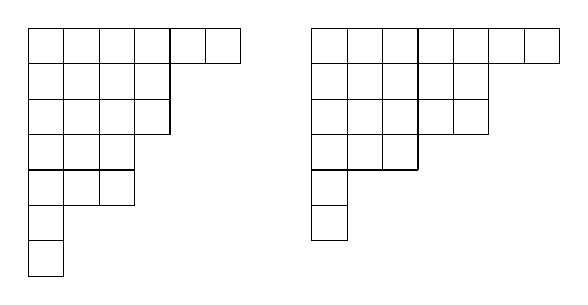
\begin{tikzpicture}[scale=0.45]
	\draw (0,0)--(6,0);
	\draw (0,-1)--(6,-1);
	\draw (0,-2)--(4,-2);
	\draw (0,-3)--(4,-3);
	\draw (0,-4)--(3,-4);
	\draw (0,-5)--(3,-5);
	\draw (0,-6)--(1,-6);
	\draw (0,-7)--(1,-7);
	\draw (0,0)--(0,-7);
	\draw (1,0)--(1,-7);
	\draw (2,0)--(2,-5);
	\draw (3,0)--(3,-5);
	\draw (4,0)--(4,-3);
	\draw (5,0)--(5,-1);
	\draw (6,0)--(6,-1);
	\draw (8,0)--(15,0);
	\draw (8,-1)--(15,-1);
	\draw (8,-2)--(13,-2);
	\draw (8,-3)--(13,-3);
	\draw (8,-4)--(11,-4);
	\draw (8,-5)--(9,-5);
	\draw (8,-6)--(9,-6);
	\draw (8,0)--(8,-6);
	\draw (9,0)--(9,-6);
	\draw (10,0)--(10,-4);
	\draw (11,0)--(11,-4);
	\draw (12,0)--(12,-3);
	\draw (13,0)--(13,-3);
	\draw (14,0)--(14,-1);
	\draw (15,0)--(15,-1);
	\end{tikzpicture}\caption{FIG.21}\label{Fig.21}
\end{wrapfigure}
with respect to the variables in different rows; alternation with respect to a pair of variables in the same row clearly gives zero identically.

Having chosen one variable from each row, we can, without loss of generality, regard them as being in the first cells in each row (after symmetrization, the order of the variables among the cells in each row is immaterial); let us alternate with respect to these variables. Having then deleted the first column, we alternate with respect to variables chosen one from each row in the thus “curtailed” diagram; these variables can again be regarded as being in the first cells of the “curtailed” rows. Continuing this process, we finally have the function first symmetrized with respect to the variables in each row and then alternated with respect to the variables in each column. After alternation, of course, the function in general ceases to be symmetrical with respect to the variables in each row. The symmetry is preserved only with respect to the variables in the cells of the first row which project beyond the other rows.

Having distributed the $ N $ variables in various ways among the rows of a Young diagram (the distribution among the cells in each row is immaterial), we thus obtain a series of functions, which are transformed linearly into one another when the variables are permuted in any manner.\footnote{It would be possible to perform the symmetrization and alternation in the reverse order: to alternate with respect to the variables in each column, and then to symmetrize with respect to those in the rows. This, however, would give effectively the same thing, since the functions obtained by the two methods are linear combinations of one another.
} However, it must be emphasized that not all these functions are linearly independent; the number of independent functions is in general less than the number of possible distributions of the variables among the rows of the diagram. We shall not pause here, however, to discuss this more closely.\footnote{The independent functions that are transformed into linear combinations of one another form the basis of an irreducible representation of the permutation group. Their number is the dimension of the representation. For particles with spin $ 1/2 $ the number is derived in Problem $ 1 $ below.}

Thus any Young diagram determines some type of symmetry of functions with respect to permutations. By constructing all the possible Young diagrams (for a given $ N $), we find all possible types of symmetry. This amounts to dividing the number N in all possible ways into a sum of smaller terms, including the number $ N $ itself; thus for $ N = 4 $ the possible partitions are $ 4, 3+1, 2+2, 2+1+1, 1+1+1+1 $.

To each energy level of the system we can make correspond a Young diagram which determines the permutational symmetry of the appropriate solutions of Schr\"odinger’s equation; in general, several different functions correspond to each value of the energy, and these are transformed linearly into each other by permutations. The existence of this “permutational degeneracy” is related to the fact that the operators $ \hat{P} $ each commute with the Hamiltonian but not with one another (see the middle of \S\ref{Stationary states}). However, it must be emphasized that this does not signify any additional physical degeneracy of the energy levels. All these different coordinate wave functions, multiplied by the spin functions, enter into a single definite combination—the complete wave function—which satisfies (according to the spin of the particles) the condition of symmetry or antisymmetry.

Among the various types of symmetry there are always (for any given $ N $) two to each of which only one function corresponds. One of these corresponds to a function symmetrical with respect to all the variables, and the other to one which is similarly antisymmetrical; in the first case, the Young diagram consists of a single row of $ N $ cells, and in the second case of a single column.

Let us now consider the spin wave functions $ \chi(\sigma_1, \sigma_2, \dots, \sigma_N) $. Their kinds of symmetry with respect to permutations of the particles are given by the same Young diagrams, with the components of the spins of the particles taking the part of variables. There arises the question of what diagram must correspond to the spin function for a given diagram of the coordinate function. Let us first suppose that the spin of the particles is integral. Then the complete wave function $\psi$ must be symmetrical with respect to all the particles. For this to be so, the symmetry of the spin and coordinate functions must be given by the same Young diagram, and the complete wave function $\psi$ is expressed as definite bilinear combinations of the two; we shall not here pause to examine more closely the problem of constructing these combinations.

Next, suppose the spin of the particles to be half-integral. Then the complete wave function must be antisymmetrical with respect to all the particles. It can be shown that, for this to be so, the Young diagrams for the coordinate and spin functions must be in dual relation, i.e. obtained from each other by interchanging rows and columns (as in the two diagrams shown in Fig. \ref{Fig.21})

Let us consider in more detail the important case of particles with spin $ 1/2 $ (electrons, for instance). Each of the spin variables $ \sigma_1, \sigma_2, \dots $ here takes only the two values $ \pm1/2 $. Since a function antisymmetrical with respect to any two variables vanishes when these variables take the same value, it is clear that the function $\chi$ can be alternated only with respect to pairs of variables; if we alternate with respect to even three variables, two of them must always take the same value, so that we have zero identically.

Thus, for a system of electrons, the Young diagrams for the spin functions can contain columns of only one or two cells (i.e. only one or two rows); in the Young diagrams for the coordinate functions, the same is true of the number of columns. The number of possible types of permutational symmetry for a system of $ N $ electrons is therefore equal to the number of possible partitions of the number $ N $ into a sum of ones and twos. When $ N $ is even, this number is $ N/2+1 $ (partitions with $ 0, 1, \dots, N/2 $ twos), while if $ N $ is odd it is $ (N+1)/2 $ (partitions with $ 0, 1, \dots, (N-1)/2 $ twos). Thus, for instance, Fig. \ref{Fig.22} shows the possible Young diagrams (coordinate and spin) for $ N = 4 $.








It is easy to see that each of these types of symmetry (i.e. each of the Young diagrams) corresponds to a definite total spin $ S $ of the system of electrons. We shall consider the spin functions in spinor form, i.e. as spinors $ \chi^{\lambda\mu\dots} $ of rank $ N $, whose indices (each of which corresponds to the spin of an individual particle) will be the variables that are arranged in the cells of the
\begin{wrapfigure}[10]{r}[0cm]{0cm}
	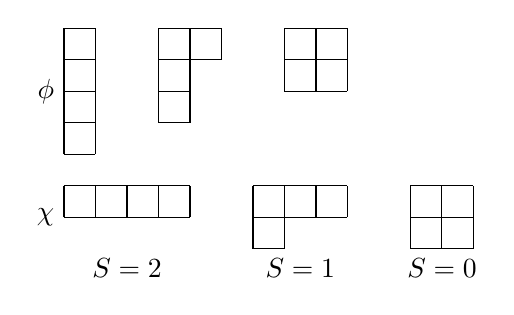
\begin{tikzpicture}[scale=0.4]
	\draw (6,0)--(7,0);
	\draw (11,0)--(13,0);
	\draw (0,1)--(4,1);
	\draw (6,1)--(9,1);
	\draw (11,1)--(13,1);
	\draw (0,2)--(4,2);
	\draw (6,2)--(9,2);
	\draw (11,2)--(13,2);
	\draw (0,3)--(1,3);
	\draw (0,4)--(1,4);
	\draw (3,4)--(4,4);
	\draw (0,5)--(1,5);
	\draw (3,5)--(4,5);
	\draw (7,5)--(9,5);
	\draw (0,6)--(1,6);
	\draw (3,6)--(5,6);
	\draw (7,6)--(9,6);
	\draw (0,7)--(1,7);
	\draw (3,7)--(5,7);
	\draw (7,7)--(9,7);
	\draw (0,1)--(0,2);
	\draw (0,3)--(0,7);
	\draw (1,1)--(1,2);
	\draw (1,3)--(1,7);
	\draw (2,1)--(2,2);
	\draw (3,1)--(3,2);
	\draw (3,4)--(3,7);
	\draw (4,1)--(4,2);
	\draw (4,4)--(4,7);
	\draw (5,6)--(5,7);
	\draw (6,0)--(6,2);
	\draw (7,0)--(7,2);
	\draw (7,5)--(7,7);
	\draw (8,1)--(8,2);
	\draw (8,5)--(8,7);
	\draw (9,1)--(9,2);
	\draw (9,5)--(9,7);
	\draw (11,0)--(11,2);
	\draw (12,0)--(12,2);
	\draw (13,0)--(13,2);
	\node[below] at (2,0) {$ S=2 $};
	\node[below] at (7.5,0) {$ S=1 $};
	\node[below] at (12,0) {$ S=0 $};
	\node[left] at (0,1) {$ \chi $};
	\node[left] at (0,5) {$ \phi $};
	\end{tikzpicture}\caption{FIG.22}\label{Fig.22}
\end{wrapfigure}
Young diagrams. Let us examine the Young diagram consisting of two rows with $ N_1 $ and $ N_2 $ cells ($ N_1+N_2 = N $, and $ N_1 \geqslant N_2 $). In each of the first $ N_2 $ columns there are two cells, and the spinor must be antisymmetrical with respect to the corresponding pairs of indices. With respect to the indices in the last $ n = N_1 - N_2 $ cells in the first row, however, it must be symmetrical. As we know, such a spinor of rank $ N $ reduces to a symmetrical spinor of rank $ n $, to which there corresponds a total spin $ S = n/2 $. Returning to the Young diagrams for the coordinate functions, we can say that the diagram with $ n $ rows each of one cell corresponds to a total spin $ S = n/2 $. For even $ N $, the total spin can take integral values from $ 0 $ to $ N/2 $, while for odd $ N $ it can take half-integral values from $ 1/2 $ to $ N/2 $, as it should.

We emphasize that this one-to-one correspondence between the Young diagrams and the total spin holds only for systems of particles with spin $ 1/2 $; we have seen this, for a system of two particles, in the previous section. For a system of $ N $ particles with spin $ s $, the spin wave function is made up of a product of $ N $ symmetrical spinors of rank $ 2s $, i.e. is a spinor of rank $ 2Ns $. If this spinor is symmetrized according to a particular Young diagram of $ N $ cells, we can usually construct from the independent components of the symmetrized spinor several sets of linear combinations, each set corresponding to a different total spin $ S $ of the system.

In the same way as the Young diagram for the spin functions of particles with spin $ 1/2 $ cannot contain columns of more than two cells, so for particles with any spin s the columns cannot contain more than $ 2s + 1 $ cells.

If the number $ N $ of particles in the system is an integral multiple of $ 2s + 1 $, the possible Young diagrams include a rectangle with $ 2s + 1 $ cells in each column. This corresponds to one definite value of the total spin, $ S = 0 $. Hence we can conclude that the same value of $ S $ corresponds to any two (spin) Young diagrams which can be fitted together to form a rectangle of height $ 2s + 1 $.\footnote{For example, the two diagrams (for $ s = 1 $):
\[ 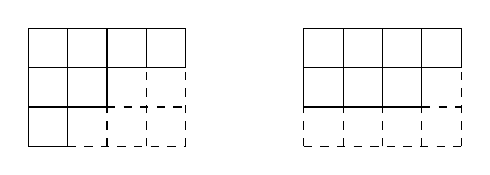
\begin{tikzpicture}[scale=0.5]
		\draw (0,3)--(4,3);
		\draw (0,2)--(4,2);
		\draw (0,1)--(2,1);
		\draw[dashed] (2,1)--(4,1);
		\draw (0,0)--(1,0);
		\draw[dashed] (1,0)--(4,0);
		\draw (0,0)--(0,3);
		\draw (1,0)--(1,3);
		\draw (2,1)--(2,3);
		\draw[dashed] (2,0)--(2,1);
		\draw (3,2)--(3,3);
		\draw[dashed] (3,0)--(3,2);
		\draw (4,2)--(4,3);
		\draw[dashed] (4,0)--(4,2);
		\draw (7,3)--(11,3);
		\draw (7,2)--(11,2);
		\draw (7,1)--(10,1);
		\draw[dashed] (10,1)--(11,1);
		\draw[dashed] (7,0)--(11,0);
		\draw[dashed] (7,0)--(7,1);
		\draw (7,1)--(7,3);
		\draw[dashed] (8,0)--(8,1);
		\draw (8,1)--(8,3);
		\draw[dashed] (9,0)--(9,1);
		\draw (9,1)--(9,3);
		\draw[dashed] (10,0)--(10,1);
		\draw (10,1)--(10,3);
		\draw[dashed] (11,0)--(11,2);
		\draw (11,2)--(11,3);
		\end{tikzpicture} \]
The continuous and broken lines show the complementary diagrams.
} This is a simple consequence of the fact that the addition of two angular momenta can give zero only if they have the same absolute magnitude.

To conclude this section, let us return to the fact already mentioned in the footnote at the end of \S\ref{The variational principle} that, for a system of several identical particles, we cannot assert that the wave function of the stationary state of lowest energy is without nodes. We can now amplify this statement and elucidate its origin.

The wave function (that is, the coordinate function), if it has no nodes, must certainly be symmetrical with respect to all the particles; for, if it were antisymmetrical with respect to the interchange of any pair of particles $ 1, 2 $, it would vanish for $ \bm{r}_1 = \bm{r}_2 $. If, however, the system consists of three or more electrons, no completely symmetrical coordinate wave function is possible (the Young diagram of the coordinate function cannot have rows with more than two cells). Thus, although the solution of Schr\"odinger’s equation which corresponds to the lowest eigenvalue is without nodes (by the theorem of the variational calculus), this solution may be physically inadmissible; the smallest eigenvalue of Schr\"odinger’s equation will not then correspond to the normal state of the system, and the wave function of this state will in general have nodes. For particles with a half-integral spin $ s $, this situation occurs in systems with more than $ 2s + 1 $ particles. For systems of bosons, a completely symmetrical coordinate wave function is always possible.





{\small
	
\textbf{PROBLEMS}


\textbf{1.}Determine the number of energy levels with different values of the total spin $ S $, for a system of $ N $ particles with spin $ 1/2 $.





SOLUTION. A given value of the projection of the total spin of the system, $ M_S = \sum \sigma $, can be obtained in
\[ f(M_S)=\frac{N!}{\left(\frac{N}{2}+M_S \right)!\left(\frac{N}{2}-M_S \right)!} \]
ways, with $ N/2 + M_S $ particles taken to have $ \sigma=1/2 $ and the remainder $ \sigma = -1/2 $. To each energy level with a given $ S $, there correspond $ 2S+1 $ states with $ M_S = S, S-1, \dots, -S $. Hence it is easy to see that the number of different energy levels with a given value of $ S $ is
\[ n(S)=f(S)-f(S+1)=\frac{N!(2S+1)}{\left(\frac{N}{2}+S+1 \right)!\left(\frac{N}{2}-S \right)!} .\]
The total number of different energy levels is
\[ n=\sum_S n(S)=f(0)=\frac{N!}{\left( \frac{N}{2}!\right)^2} \]
for even $ N $, and
\[ n=f\left(\frac{1}{2}\right)=\frac{N!}{\left(\frac{N+1}{2} \right)!\left(\frac{N-1}{2} \right)!} \]
for odd $ N $.





\textbf{2.} Find the values of the total spin $ S $ that occur for various types of symmetry of the spin functions of a system of two, three or four particles with spin $ 1 $.





SOLUTION. For two particles, the correspondence is established by the fact that the factor by which the spin function is multiplied when the particles are interchanged must be $ (-1)^{2s-S} $ (see the end of \S\ref{Exchange interaction}). For particles with spin $ s = 1 $ this gives
\begin{equation}\label{63-2-1}
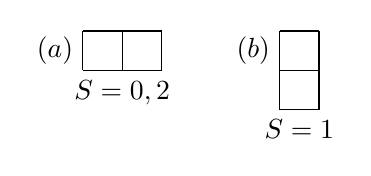
\begin{tikzpicture}[baseline,scale=0.5]
\draw (0,0)--(2,0);
\draw (0,1)--(2,1);
\draw (5,-1)--(6,-1);
\draw (5,0)--(6,0);
\draw (5,1)--(6,1);
\draw (0,0)--(0,1);
\draw (1,0)--(1,1);
\draw (2,0)--(2,1);
\draw (5,-1)--(5,1);
\draw (6,-1)--(6,1);
\node[below] at (1,0) {$ S=0,2 $};
\node[below] at (5.5,-1) {$ S=1 $};
\node[left] at (0,0.5) {$ (a) $};
\node[left] at (5,0.5) {$ (b) $}; 
\end{tikzpicture}\tag{1}
\end{equation}



The Young diagrams for a system of three particles are obtained by adding to the diagrams \eqref{63-2-1} one cell in every possible way. The result may be written as the symbolic equations
\[ 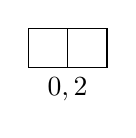
\begin{tikzpicture}[baseline,scale=0.5]
\draw (0,0)--(2,0);
\draw (0,1)--(2,1);
\draw (0,0)--(0,1);
\draw (1,0)--(1,1);
\draw (2,0)--(2,1);
\node[below] at (1,0) {$ 0,2 $};
\end{tikzpicture}\quad\times\quad\begin{tikzpicture}[baseline,scale=0.5]
\draw (0,0)--(1,0);
\draw (0,0)--(0,1);
\draw (1,0)--(1,1);
\draw (0,1)--(1,1);
\node[below] at (0.5,0) {$ 1 $};
\end{tikzpicture}\quad=\quad\underbrace{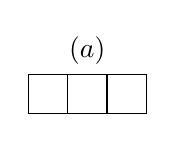
\begin{tikzpicture}[baseline,scale=0.5]
	\draw (0,0)--(3,0);
	\draw (0,0)--(0,1);
	\draw (1,0)--(1,1);
	\draw (2,0)--(2,1);
	\draw (3,0)--(3,1);
	\draw (0,1)--(3,1);
	\node[above] at (1.5,1) {$ (a) $};
	\end{tikzpicture}\quad+\quad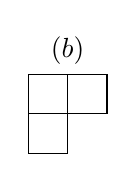
\begin{tikzpicture}[baseline,scale=0.5]
	\draw (0,0)--(2,0);
	\draw (0,-1)--(0,1);
	\draw (1,-1)--(1,1);
	\draw (2,0)--(2,1);
	\draw (0,1)--(2,1);
	\draw (2,0)--(2,1);
	\draw (0,-1)--(1,-1);
	\node[above] at (1,1) {$ (b) $};
	\end{tikzpicture}}_{1,1,2,3} \]
\[ 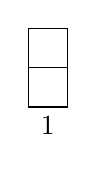
\begin{tikzpicture}[baseline,scale=0.5]
\draw (0,-1)--(0,1);
\draw (1,-1)--(1,1);
\draw (0,1)--(1,1);
\draw (0,0)--(1,0);
\draw (0,-1)--(1,-1);
\node[below] at (0.5,-1) {$ 1 $};
\end{tikzpicture}\quad\times\quad\begin{tikzpicture}[baseline,scale=0.5]
\draw (0,0)--(0,1);
\draw (1,0)--(1,1);
\draw (0,1)--(1,1);
\draw (0,0)--(1,0);
\node[below] at (0.5,-1) {$ 1 $};
\end{tikzpicture}\quad=\quad\underbrace{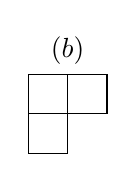
\begin{tikzpicture}[baseline,scale=0.5]
	\draw (0,-1)--(0,1);
	\draw (1,-1)--(1,1);
	\draw (2,0)--(2,1);
	\draw (0,-1)--(1,-1);
	\draw (0,0)--(2,0);
	\draw (0,1)--(2,1);
	\node[above] at (1,1) {$ (b) $};
	\end{tikzpicture}\quad+\quad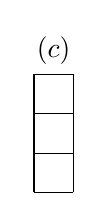
\begin{tikzpicture}[baseline,scale=0.5]
	\draw (0,-2)--(0,1);
	\draw (1,-2)--(1,1);
	\draw (0,1)--(1,1);
	\draw (0,0)--(1,0);
	\draw (0,-1)--(1,-1);
	\draw (0,-2)--(1,-2);
	\node[above] at (0.5,1) {$ (c) $};
	\end{tikzpicture}}_{0,1,2}
 \]
The values of $ S $ are shown beneath each diagram, and the values of the total spin of the system of three particles (the diagrams on the right) are found from the spins of the two-particle and one-particle systems (the diagrams on the left) by the rule of addition of angular momenta.\footnote{The repetition of $ 1 $ beneath the right-hand diagrams occurs because this value of the angular momentum comes firstly from adding the angular momenta $ 0 $ and $ 1 $, and secondly from adding $ 2 $ and $ 1 $.
} The distribution of the resulting values of $ S $ among the diagrams on the right is established by noting that diagram $ (c) $ (a column of three cells) corresponds to $ S = 0 $, and $ (b) $ therefore to the remaining values $ 1 $ and $ 2 $ in the second equation, while $ (a) $ belongs to the values $ 1 $ and $ 3 $ that are left after $ (b) $ has been labelled in the first equation:
\begin{equation}\label{63-2-2}
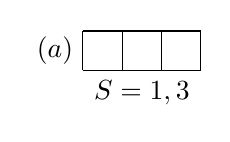
\begin{tikzpicture}[baseline,scale=0.5]
\draw (0,1)--(3,1);
\draw (0,2)--(3,2);
\draw (0,1)--(0,2);
\draw (1,1)--(1,2);
\draw (2,1)--(2,2);
\draw (3,1)--(3,2);
\node[left] at (0,1.5) {$ (a) $};
\node[below] at (1.5,1) {$ S=1,3 $};
\end{tikzpicture}\qquad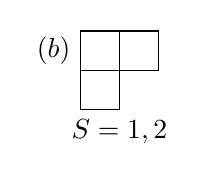
\begin{tikzpicture}[baseline,scale=0.5]
\draw (0,1)--(2,1);
\draw (0,2)--(2,2);
\draw (0,0)--(1,0);
\draw (0,0)--(0,2);
\draw (1,0)--(1,2);
\draw (2,1)--(2,2);
\node[left] at (0,1.5) {$ (b) $};
\node[below] at (1,0) {$ S=1,2 $};
\end{tikzpicture}\qquad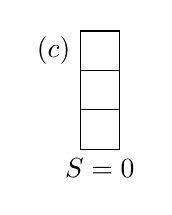
\begin{tikzpicture}[baseline,scale=0.5]
\draw (0,-1)--(0,2);
\draw (1,-1)--(1,2);
\draw (0,-1)--(1,-1);
\draw (0,0)--(1,0);
\draw (0,1)--(1,1);
\draw (0,2)--(1,2);
\node[left] at (0,1.5) {$ (c) $};
\node[below] at (0.5,-1) {$ S=0 $};
\end{tikzpicture}\tag{2}
\end{equation}
The Young diagrams for a system of four particles are obtained by adding one cell to the diagrams \eqref{63-2-2}, with the condition that no column should contain more than three cells:
\begin{equation*}
\begin{split}
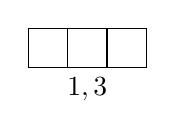
\begin{tikzpicture}[baseline,scale=0.5]
\draw (0,0)--(3,0);
\draw (0,1)--(3,1);
\draw (0,0)--(0,1);
\draw (1,0)--(1,1);
\draw (2,0)--(2,1);
\draw (3,0)--(3,1);
\node[below] at (1.5,0) {$ 1,3 $};
\end{tikzpicture}\quad\times\quad\begin{tikzpicture}[baseline,scale=0.5]
\draw (0,0)--(0,1);
\draw (0,1)--(1,1);
\draw (1,0)--(1,1);
\draw (0,0)--(1,0);
\node[below] at (0.5,0) {$ 1 $};
\end{tikzpicture}\quad&=\quad\underbrace{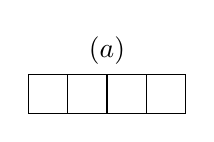
\begin{tikzpicture}[baseline,scale=0.5]
	\draw (0,0)--(4,0);
	\draw (0,1)--(4,1);
	\draw (0,0)--(0,1);
	\draw (1,0)--(1,1);
	\draw (2,0)--(2,1);
	\draw (3,0)--(3,1);
	\draw (4,0)--(4,1);
	\node[above] at (2,1) {$ (a) $};
	\end{tikzpicture}\quad+\quad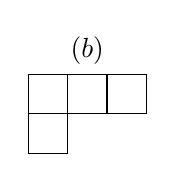
\begin{tikzpicture}[baseline,scale=0.5]
	\draw (0,0)--(3,0);
	\draw (0,1)--(3,1);
	\draw (0,-1)--(1,-1);
	\draw (0,-1)--(0,1);
	\draw (1,-1)--(1,1);
	\draw (2,0)--(2,1);
	\draw (3,0)--(3,1);
	\node[above] at (1.5,1) {$ (b) $};
	\end{tikzpicture}}_{0,1,2,2,3,4}\\
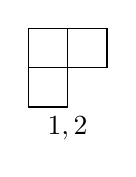
\begin{tikzpicture}[baseline,scale=0.5]
\draw (0,0)--(2,0);
\draw (0,1)--(2,1);
\draw (0,-1)--(1,-1);
\draw (0,-1)--(0,1);
\draw (1,-1)--(1,1);
\draw (2,0)--(2,1);
\node[below] at (1,-1) {$ 1,2 $}; 
\end{tikzpicture}\quad\times\quad\begin{tikzpicture}[baseline,scale=0.5]
\draw (0,0)--(1,0);
\draw (1,0)--(1,1);
\draw (0,1)--(1,1);
\draw (0,0)--(0,1);
\node[below] at (0.5,-1) {$ 1 $};
\end{tikzpicture}\quad&=\quad\underbrace{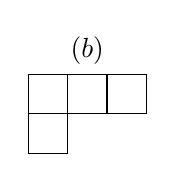
\begin{tikzpicture}[baseline,scale=0.5]
	\draw (0,0)--(3,0);
	\draw (0,1)--(3,1);
	\draw (0,-1)--(1,-1);
	\draw (0,-1)--(0,1);
	\draw (1,-1)--(1,1);
	\draw (2,0)--(2,1);
	\draw (3,0)--(3,1);
	\node[above] at (1.5,1) {$ (b) $};
	\end{tikzpicture}\quad+\quad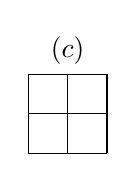
\begin{tikzpicture}[baseline,scale=0.5]
	\draw (0,0)--(2,0);
	\draw (0,1)--(2,1);
	\draw (0,-1)--(2,-1);
	\draw (0,-1)--(0,1);
	\draw (1,-1)--(1,1);
	\draw (2,-1)--(2,1);
	\node[above] at (1,1) {$ (c) $};
	\end{tikzpicture}\quad+\quad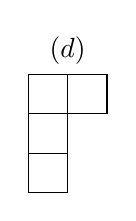
\begin{tikzpicture}[baseline,scale=0.5]
	\draw (0,0)--(2,0);
	\draw (0,1)--(2,1);
	\draw (0,-1)--(1,-1);
	\draw (0,-2)--(1,-2);
	\draw (0,-2)--(0,1);
	\draw (1,-2)--(1,1);
	\draw (2,0)--(2,1);
	\node[above] at (1,1) {$ (d) $};
	\end{tikzpicture}}_{0,1,1,2,2,3}\\
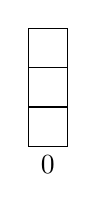
\begin{tikzpicture}[baseline,scale=0.5]
\draw (0,-2)--(0,1);
\draw (1,-2)--(1,1);
\draw (0,-2)--(1,-2);
\draw (0,-1)--(1,-1);
\draw (0,0)--(1,0);
\draw (0,1)--(1,1);
\node[below] at (0.5,-2) {$ 0 $};
\end{tikzpicture}\quad\times\quad\begin{tikzpicture}[baseline,scale=0.5]
\draw (0,0)--(1,0);
\draw (0,0)--(0,1);
\draw (1,0)--(1,1);
\draw (0,1)--(1,1);
\node[below] at (0.5,0) {$ 1 $};
\end{tikzpicture}\quad&=\quad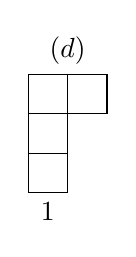
\begin{tikzpicture}[baseline,scale=0.5]
\draw (0,1)--(2,1);
\draw (0,0)--(2,0);
\draw (0,-1)--(1,-1);
\draw (0,-2)--(1,-2);
\draw (0,-2)--(0,1);
\draw (1,-2)--(1,1);
\draw (2,0)--(2,1);
\node[above] at (1,1) {$ (d) $};
\node[below] at (0.5,-2) {$ 1 $};
\end{tikzpicture}
\end{split}
\end{equation*}
Diagram $ (c) $ can be added to $ (a) $ in $ (1) $ to form a rectangle with three-cell columns, and therefore corresponds to the same values $ S = 0, 2 $. The values of $ S $ for diagram $ (b) $ are found from the remainder of the second equation, and then those for $ (a) $ from the remainder of the first equation:
\[ 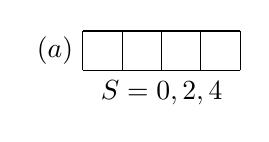
\begin{tikzpicture}[baseline,scale=0.5]
\draw (0,0)--(4,0);
\draw (0,1)--(4,1);
\draw (0,0)--(0,1);
\draw (1,0)--(1,1);
\draw (2,0)--(2,1);
\draw (3,0)--(3,1);
\draw (4,0)--(4,1);
\node[left] at (0,0.5) {$ (a) $};
\node[below] at (2,0) {$ S=0,2,4 $};
\end{tikzpicture}\qquad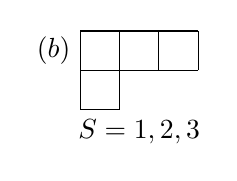
\begin{tikzpicture}[baseline,scale=0.5]
\draw (0,0)--(3,0);
\draw (0,1)--(3,1);
\draw (0,-1)--(1,-1);
\draw (0,-1)--(0,1);
\draw (1,-1)--(1,1);
\draw (2,0)--(2,1);
\draw (3,0)--(3,1);
\node[left] at (0,0.5) {$ (b) $};
\node[below] at (1.5,-1) {$ S=1,2,3 $};
\end{tikzpicture}\qquad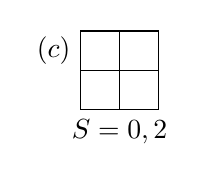
\begin{tikzpicture}[baseline,scale=0.5]
\node[left] at (0,0.5) {$ (c) $};
\draw (0,1)--(2,1);
\draw (0,0)--(2,0);
\draw (0,-1)--(2,-1);
\draw (0,-1)--(0,1);
\draw (1,-1)--(1,1);
\draw (2,-1)--(2,1);
\node[below] at (1,-1) {$ S=0,2 $};
\end{tikzpicture}\qquad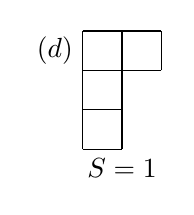
\begin{tikzpicture}[baseline,scale=0.5]
\draw (0,0)--(2,0);
\draw (0,1)--(2,1);
\draw (0,-1)--(1,-1);
\draw (0,-2)--(1,-2);
\draw (0,-2)--(0,1);
\draw (1,-2)--(1,1);
\draw (2,0)--(2,1);
\node[left] at (0,0.5) {$ (d) $};
\node[below] at (1,-2) {$ S=1 $};
\end{tikzpicture} \]
}
\section{Second quantization. The case of Bose statistics}\label{Second quantization. The case of Bose statistics}
In the theory of systems consisting of a large number of identical particles, there is a widely used method of considering the problem, known as \textit{second quantization}. This method is especially necessary in relativistic theory, where we have to deal with systems in which the number of particles is itself variable.\footnote{The method of second quantization was developed by P. A. M. Dirac (1927) for photons in radiation theory, and later extended to fermions by E. Wigner and P. Jordan (1928).
}

Let $ \psi_1(\xi), \psi_2(\xi), \dots $ be some complete set of orthogonal and normalized wave functions of stationary states of a single particle.\footnote{As in \S\ref{The principle of indistinguishability of similar particles}, $\xi$ denotes the set of the coordinates and the spin projection $\sigma$ of the particle, and integration with respect to $\xi$ is taken to mean integration over the coordinates and summation over $\sigma$.
} These may be states of a particle in some arbitrarily chosen external field, but are usually taken to be simply plane waves, i.e. the wave functions of a free-particle having definite values of the momentum (and spin projection). In order to make the spectrum of states discrete, we shall consider the motion of particles in a large but finite region, for which the eigenvalues of the momentum components form a discrete series, the intervals between adjacent values being inversely proportional to the linear dimensions of the region and tending to zero as these increase.

In a system of free particles, the particle momenta are separately conserved. The occupation numbers of the states are therefore also conserved, i.e. the numbers $ N_1, N_2, \dots $ which show how many particles are in each of the states $ \psi_1, \psi_2, \dots $. In a system of interacting particles, the momentum of each particle is not conserved, and so the occupation numbers are not conserved. For such a system we can consider only the probability distribution of the various values of the occupation numbers. Let us seek to construct a mathematical formalism in which the occupation numbers (and not the coordinates and spin projections of the particles) play the part of independent variables.

In this formalism, it is convenient to use the Dirac notation (see the end of \S\ref{Matrices}), taking $ N_1, N_2, \dots $ as quantum numbers defining the state. The states corresponding to the wave functions \eqref{61.3} and \eqref{61.5} will be denoted by $ \left|N_1, N_2, \dots\> $. The coordinate and spin variables of the particles are not shown explicitly.

In accordance with this choice of the independent variables, the operators of the various physical quantities (including the Hamiltonian of the system) must be formulated in terms of their action on functions of the occupation numbers. Such a formulation can be obtained on the basis of the usual matrix representation of operators. The operator matrix elements must be considered in relation to the wave functions of the stationary states of a system of non-interacting particles. Since these states can be described by specifying definite values of the occupation numbers, this will also show the nature of the action of the operators on these variables.

Let us first consider systems of particles obeying Bose statistics. Let $ \hat{f}_a^{(1)} $ be the operator of some quantity pertaining to the $ a $th particle, i.e. acting only on functions of the variables $\xi_a$. We introduce the operator
\begin{equation}\label{64.1}
\hat{F}^{(1)}=\sum_a\hat{f}_a^{(1)}
\end{equation}
which is symmetrical with respect to all the particles (the summation being over all particles), and determine its matrix elements with respect to the wave functions \eqref{61.3}. First of all, it is easy to see that the matrix elements will be different from zero only for transitions which leave the numbers $ N_1, N_2, \dots $ unchanged (diagonal elements) and for transitions where one of these numbers is increased, and another decreased, by unity. For, since each of the operators $ \hat{f}_a^{(1)} $ acts only on one function in the product $ \psi_{p_1}(\xi_1)\psi_{p_2}(\xi_2)\dots \psi_{p_N}(\xi_N) $, its matrix elements can be different from zero only for transitions whereby the state of a single particle is changed; this, however, means that the number of particles in one state is diminished by unity, while the number in another state is correspondingly increased. The calculation of these matrix elements is in principle very simple; it is easier to do it oneself than to follow an account of it. Hence we shall give only the result of this calculation. The non-diagonal elements are
\begin{equation}\label{64.2}
\< N_i,N_k-1|F^{(1)}|N_i-1,N_k\>=f_{ik}^{(1)}\sqrt{N_iN_k}.
\end{equation}
We shall indicate only those suffixes with respect to which the matrix element is non-diagonal, omitting the remainder for brevity. Here $ f_{ik}^{(1)} $ is the matrix element
\begin{equation}\label{64.3}
f_{ik}^{(1)}=\int\psi_i^*(\xi)\hat{f}^{(1)}\psi_k(\xi)\d\xi;
\end{equation}
since the operators $ f_a^{(1)} $ differ only in the naming of the variables on which they act, the integrals \eqref{64.3} are independent of a, which is therefore omitted. The diagonal matrix elements of $ F^{(1)} $ are the mean values of the quantity $ F^{(1)} $ in the states $ \Psi_{N_1N_2\dots} $. Calculation gives
\begin{equation}\label{64.4}
\bar{F^{(1)}}=\sum_i f_{ii}^{(1)}N_i.
\end{equation}



We now introduce the operators $ \hat{a}_i $, which play a leading part in the method of second quantization; they act, not on functions of the coordinates, but on functions of the occupation numbers. By definition, the operator $ \hat{a}_i $ acting on the function $ \left|N1, N2, \dots\> $ decreases the value of the variable $ N_i $ by unity, and at the same time it multiplies the function by $\sqrt{N_i}$:\footnote{Here we use the notation $ \hat{a}\left|m\> $ with the natural sense of the result of the operator $\hat{a}$ acting on the state wave function $ \left|m\>. $
}
\begin{equation}\label{64.5}
\hat{a}_i\left|N_1,N_2,\dots,N_i,\dots\>=\sqrt{N_i}\left|N_1,N_2,\dots,N_i-1,\dots\>.
\end{equation}
We can say that the operator $\hat{a}_i$ diminishes by one the number of particles in the $ i $th state; it is therefore called a particle \textit{annihilation operator}. It can be represented in the form of a matrix whose only non-zero element is
\begin{equation}\label{64.6}
\< N_i-1|a_i|N_i\>=\sqrt{N_i}.
\end{equation}


The operator $ \hat{a}_i^\dagger $ which is the Hermitian conjugate of $ \hat{a}_i $ is, by definition (see \eqref{11.9}), represented by a matrix whose only non-zero element is
\begin{equation}\label{64.7}
\<N_i\right|a_i^\dagger\left|N_i-1\>=\<N_i-1|a_i|N_i\>^*=\sqrt{N_i}
\end{equation}
This means that, when acting on the function $ \Phi(N_1, N_2, \dots) $. it increases the number $ N_i $ by unity:
\begin{equation}\label{64.8}
\hat{a}_i^\dagger\left|N_1,N_2,\dots,N_i,\dots\>=\sqrt{N_i+1}\left|N_1,N_2,\dots,N_i+1,\dots\>.
\end{equation}
In other words, the operator $\hat{a}_i^\dagger$ increases by one the number of particles in the $ i $th state, and is therefore called a particle \textit{creation operator}.

The product of the operators $ \hat{a}_i^\dagger\hat{a}_i $, acting on the wave function, must multiply it by a constant simply, leaving unchanged all the variables $ N_1, N_2, \dots $: the operator $\hat{a}_i$ diminishes $ N_i $ by unity, and $\hat{a}_i^\dagger$ then restores it to its original value. Direct multiplication of the matrices \eqref{64.6} and \eqref{64.7} shows that $ \hat{a}_i^\dagger\hat{a}_i $ is represented, as we should expect, by a diagonal matrix whose diagonal elements are $ N_i $. We can write
\begin{equation}\label{64.9}
 \hat{a}_i^\dagger\hat{a}_i =N_i.
\end{equation}
Similarly, we find that
\begin{equation}\label{64.10}
\hat{a}_i\hat{a}_i^\dagger=N_i+1.
\end{equation}



The difference of these equations gives the commutation rule for the operators $\hat{a}_i$ and $ \hat{a}_i^\dagger $:
\begin{equation}\label{64.11}
\hat{a}_i\hat{a}_i^\dagger-\hat{a}_i^\dagger\hat{a}_i=1.
\end{equation}
The operators with $ i $ and $ k $ different act on different variables ($ N_i $ and $ N_k $), and commute:
\begin{equation}\label{64.12}
\hat{a}_i\hat{a}_k-\hat{a}_k\hat{a}_i=0,\quad\hat{a}_i\hat{a}_k^\dagger-\hat{a}_k^\dagger\hat{a}_i=0,\quad i\ne k.
\end{equation}



From the above properties of the operators $ \hat{a}_i, \hat{a}_i^\dagger $ it is easy to see that the operator
\begin{equation}\label{64.13}
\hat{F}^{(1)}=\sum_{i,k}=f_{ik}^{(1)}\hat{a}_i^\dagger\hat{a}_k
\end{equation}
is the same as the operator \eqref{64.1}. For all the matrix elements calculated from \eqref{64.6}, \eqref{64.7} are the same as the elements \eqref{64.2}, \eqref{64.4}. This is a very important result. In formula \eqref{64.13}, the quantities $ f^{(1)}_{ik} $ are simply numbers. Thus we have been able to express an ordinary operator, acting on functions of the coordinates, in the form of an operator acting on functions of new variables, the occupation numbers $ N_i $.

The result which we have obtained is easily generalized to operators of other forms. Let
\begin{equation}\label{64.14}
\hat{F}^{(2)}=\sum_{a>b}\hat{f}_{ab}^{(2)},
\end{equation}
where $ \hat{f}_{ab}^{(2)} $ is the operator of a physical quantity pertaining to two particles at once, and hence acts on functions of $\xi_a$ and $\xi_b$. Similar calculations show that this operator can be expressed in terms of the operators $ \hat{a}_i, \hat{a}_i^\dagger $ by
\begin{equation}\label{64.15}
\hat{F}^{(2)}=\frac{1}{2}\sum_{i,k,l,m}\< ik|f^{(2)}|lm\>\hat{a}_i^\dagger\hat{a}_k^\dagger\hat{a}_m\hat{a}_l,
\end{equation}
where
\[ \< ik|f^{(2)}|lm\>=\iint\psi_i^*(\xi_1)\psi_k^*(\xi_2)\hat{f}^{(2)}\psi_l(\xi_1)\psi_m(\xi_2)\d\xi_1\d\xi_2. \]
The generalization of these formulae to operators of any other form symmetrical with respect to all the particles (of the form $ \hat{F}^{(3)} = \sum\hat{f}^{(3)}_{abc} $, etc.) is obvious.

These formulae can be used to express, in terms of the operators $\hat{a}_i$ and $\hat{a}_i^\dagger$, the Hamiltonian of the physical system of $ N $ identical interacting particles that is being considered. The Hamiltonian of such a system is, of course, symmetrical with respect to all the particles. In the non-relativistic approximation,\footnote{n the absence of a magnetic field.} it is independent of the spins of the particles, and can be represented in a general form as follows:
\begin{equation}\label{64.16}
\hat{H}=\sum_a\hat{H}_a^{(1)}+\sum_{a>b}U^{(2)}(\bm{r}_a,\bm{r}_b)+\sum_{a>b>c}U^{(3)}(\bm{r}_a,\bm{r}_b,\bm{r}_c)+\dots
\end{equation}
Here $ \hat{H}^{(1)}_a $ is the part of the Hamiltonian which depends on the coordinates of the $ a $th particle only:
\begin{equation}\label{64.17}
\hat{H}_a^{(1)}=-\frac{\h^2}{2m}\Delta_a+U^{(1)}(\bm{r}_a).
\end{equation}
where $ U^{(1)}(\bm{r}_a) $ is the potential energy of a single particle in the external field. The remaining terms in \eqref{64.16} correspond to the mutual interaction energy of the particles; the terms depending on the coordinates of two, three, etc. particles have been separated.

This representation of the Hamiltonian enables us to apply formulae \eqref{64.13}, \eqref{64.15} and their analogues directly. Thus
\begin{equation}\label{64.18}
\hat{H}=\sum_{i,k}H_{ik}^{(1)}\hat{a}_i^\dagger\hat{a}_k+\frac{1}{2}\sum_{i,k,l,m}\< ik|U^{(2)}|lm\>\hat{a}_i^\dagger\hat{a}_k^\dagger\hat{a}_m\hat{a}_l\dots
\end{equation}
This gives the required expression for the Hamiltonian in the form of an operator acting on functions of the occupation numbers.

For a system of non-interacting particles, only the first term in the expression \eqref{64.18} remains:
\begin{equation}\label{64.19}
\hat{H}=\sum_{i,k}H_{ik}^{(1)}\hat{a}_i^\dagger\hat{a}_k.
\end{equation}
If the functions $\psi_i$ are taken to be the eigenfunctions of the Hamiltonian $ \hat{H}^{(1)} $ of an individual particle, the matrix $ \hat{H}^{(1)}_{ik} $ is diagonal, and its diagonal elements are the eigenvalues $ \epsilon_i $ of the energy of the particle. Thus,
\[ \hat{H}=\sum_i\epsilon_i\hat{a}_i^\dagger\hat{a}_i; \]
replacing the operator $ \hat{a}_i^\dagger\hat{a}_i $ by its eigenvalues \eqref{64.9}, we have for the energy levels of the system the expression
\[ E=\sum_i\epsilon_i N_i \]
a trivial result which could have been foreseen.

The formalism which we have developed can be put in a more compact form by introducing the $\psi$-\textit{operators}\footnote{Note the analogy between \eqref{64.20} and the expansion
\[ \psi=\sum a_i\psi_i \]	
of any wave function in terms of a complete set of functions. Here it is “re-quantized”, and this is the reason for the term \textit{second quantization method}.}
\begin{equation}\label{64.20}
\hat{\psi}(\xi)=\sum_i\psi_i(\xi)\hat{a}_i\quad\hat{\psi}^\dagger(\xi)=\sum_i\psi^*(\xi)\hat{a}_i^\dagger,
\end{equation}
where the variables $\xi$ are regarded as parameters. By what has been said above concerning the operators $ \hat{a}_i, \hat{a}_i^\dagger $, it is clear that the operator $\hat{\psi}$ decreases the total number of particles in the system by one, while $\hat{\psi}^\dagger$ increases it by one.

It is easy to see that the operator $ \hat{\psi}^\dagger(\xi_0) $ creates a particle at the point $\xi_0$. For the result of the action of the operator $\hat{a}_i^\dagger$ is to create a particle in a state with wave function $\psi_i(\xi)$. Hence it follows that the result of the action of the operator $ \hat{\psi}^\dagger(\xi_0) $ is to create a particle in a state with wave function \[ \sum_i\psi_i^*(\xi)\psi_i(\xi_0)=\delta(\xi-\xi_0) , \] 
which corresponds to a particle with definite values of the coordinates (and spin). Here we have used formula \eqref{5.12}.\footnote{$ \delta(\xi-\xi_0) $ conventionally denotes the product
\[ \delta(x-x_0)\delta(y-y_0)\delta(z-z_0)\delta_{\sigma\sigma_0}. \]}

The commutation rules for the $\psi$ operators are obtained at once from those for the operators $ \hat{a}_i, \hat{a}_i^\dagger $:
\begin{equation}\label{64.21}
\hat{\psi}(\xi)\hat{\psi}(\xi')-\hat{\psi}(\xi')\hat{\psi}(\xi)=0,
\end{equation}
\begin{equation}\label{64.22}
\hat{\psi}(\xi)\hat{\psi}^\dagger(\xi')-\hat{\psi}^\dagger(\xi')\hat{\psi}(\xi)=\sum_i\psi_i(\xi)\psi_i^*(\xi')=\delta(\xi-\xi').
\end{equation}




The second-quantized operator $ \hat{F}^{(1)} $ can be written by means of the $\psi$ operators in the form
\begin{equation}\label{64.23}
\hat{F}^{(1)}=\int\hat{\psi}^\dagger(\xi)\hat{f}^{(1)}\hat{\psi}(\xi)\d\xi
\end{equation}
where it is understood that the operator $ \hat{f}^{(1)} $ acts on functions of the parameters $\xi$ in $\hat{\psi}(\xi)$. For, substituting $\hat{\psi}$ and $\hat{\psi}^\dagger$ in the form \eqref{64.20} and using the definition \eqref{64.3}, we return to \eqref{64.13}. Similarly, \eqref{64.15} becomes
\begin{equation}\label{64.24}
\hat{F}^{(2)}=\frac{1}{2}\iint\hat{\psi}^\dagger(\xi)\hat{\psi}^\dagger(\xi')\hat{f}^{(2)}\hat{\psi}(\xi')\hat{\psi}(\xi)\d\xi\d\xi'.
\end{equation}



In particular, the Hamiltonian of the system, expressed in terms of the $\psi$ operators, is
\begin{multline}\label{64.25}
\hat{H}=\int\left\{-\frac{\h^2}{2m}\hat{\psi}^\dagger(\xi)\Delta\hat{\psi}(\xi)+\hat{\psi}^\dagger(\xi)U^{(1)}(\xi)\hat{\psi}(\xi) \right\}\d\xi+\\
+\frac{1}{2}\iint\hat{\psi}^\dagger(\xi)\hat{\psi}^\dagger(\xi')U^{(2)}(\xi,\xi')\hat{\psi}(\xi')\hat{\psi}(\xi)\d\xi\d\xi'+\dots
\end{multline}



The operator $ \hat{\psi}^\dagger(\xi)\hat{\psi}(\xi) $, constructed from the $\psi$ operators by analogy with the product $ \psi^*\psi $ which determines the probability density for a particle in a state with wave function $\psi$, is called the \textit{particle density operator}. The integral
\begin{equation}\label{64.26}
\hat{N}=\int\hat{\psi}^\dagger\hat{\psi}\d\xi
\end{equation}
represents in the second-quantization formalism the operator of the total number of particles in the system. For, substituting the $\psi$ operators in the form \eqref{64.20} and using the normalization and the orthogonality of the wave functions, we have
\[ \hat{N}=\sum\hat{a}_i^\dagger\hat{a}_i. \]
Each term in this sum is the operator of the number of particles in the ith state; according to \eqref{64.9}, its eigenvalues are equal to the occupation numbers $ N_i $, and the sum of all these numbers is the total number of particles in the system.\footnote{For systems containing a specified number of particles these statements are trivial, as are the properties of the Hamiltonian \eqref{64.19} of a system of free particles. Their generalization in the relativistic theory, however, yields new results that are by no means trivial (cf. RQT, \S11)
}

Lastly, if the system consists of bosons of various kinds, operators $\hat{a}$ and $\hat{a}^\dagger$ for each kind of particle must be defined in the second quantization method. It is evident that operators pertaining to particles of different kinds commute.
\section{Second quantization. The case of Fermi statistics}\label{Second quantization. The case of Fermi statistics}
The basic theory of the method of second quantization remains wholly unchanged for systems of identical fermions, but the actual formulae for the matrix elements of quantities and for the operators $ \hat{a}_i $ are naturally different.

The wave function $ \psi_{N_1N_2\dots} $ now has the form \eqref{61.5}. Because of the antisymmetry of this function, the question of its sign arises first of all. This question did not arise in the case of Bose statistics, since, because of the symmetry of the wave function, its sign, once chosen, was preserved under all permutations of the particles. In order to make definite the sign of the function \eqref{61.5}, we shall agree to choose it as follows. We number successively, once and for all, all the states $\psi_i$. We then complete the rows of the determinant \eqref{61.5} so that always
\begin{equation}\label{65.1}
p_1<p_2<p_3<\dots<p_N,
\end{equation}
whilst in the successive columns we have functions of the different variables in the order $ \xi_1,\xi_2,\dots,\xi_N $. No two of the numbers $ p_1, p_2, \dots $ can be equal, since otherwise the determinant would vanish. In other words, the occupation numbers $ N_i $ can take only the values $ 0 $ and $ 1 $.

Let us again consider an operator of the form \eqref{64.1}, $ \hat{F}^{(1)}=\sum\hat{f}_a^{(1)} $. As in \S\ref{Second quantization. The case of Bose statistics}, its matrix elements will be non-zero only for transitions where all the occupation numbers remain unchanged and for those where one occupation number $ (N_i) $ is diminished by unity (becoming zero instead of one) and another $ (N_k) $ is increased by unity (becoming one instead of zero). We easily find that, for $ i < k $,
\begin{equation}\label{65.2}
\<1_i,0_k|F^{(1)}|0_i,1_k\>=f_{ik}^{(1)}(-1)^{\sum(i+1,k-1)}.
\end{equation}
where by $ 0_i, 1_i $ we signify $ N_i = 0 $, $ N_i = 1 $ and the symbol $ \sum(k,l) $ denotes the sum of the occupation numbers of all states from the $ k $th to the $ l $th:\footnote{For $ i > k $ the exponent in \eqref{65.2} becomes $ \sum(k+1,i-1) $. The sum must be taken as zero when $ i = k\pm1 $.}
\[ \sum(k,l)=\sum_{n=k}^l N_n. \]
For the diagonal elements we obtain our previous formula \eqref{64.4}:
\begin{equation}\label{65.3}
\bar{F^{(1)}}=\sum_i f_{ii}^{(1)}N_i
\end{equation}



In order to represent the operator $ \hat{F}^{(1)} $ in the form \eqref{64.13}, the operators $\hat{a}_i$ must be defined as matrices whose elements are
\begin{equation}\label{65.4}
\<0_i|a_i|1_i\>=\<1_i\right|a_i^\dagger\left|0_i\>=(-1)^{\sum(1,i-1)}.
\end{equation}
On multiplying these matrices, we find, for $ k > i $,
\begin{multline*}
\<1_i,0_k\right|a_i^\dagger a_k\left|0_i,1_k\>=\<1_i,0_k\right|a_i^\dagger\left|0_i,0_k\>\<0_i,0_k|a_k|0_i,1_k\>=\\
=(-1)^{\sum(1,i-1)}(-1)^{\sum(1,i-1)+\sum(i+1,k-1)}
\end{multline*}
or
\begin{equation}\label{65.5}
\<1_i,0_k\right|a_i^\dagger a_k\left|0_i,1_k\>=(-1)^{\sum(i+1,k-1)}.
\end{equation}
If $ i = k $, the matrix of $ \hat{a}_i^\dagger\hat{a}_i $ is diagonal, and its elements are unity for $ N_i = 1 $, and zero for $ N_i = 0 $; this can be written
\begin{equation}\label{65.6}
\hat{a}_i^\dagger\hat{a}_i=N_i.
\end{equation}
On substituting these expressions in \eqref{64.13}, we in fact obtain \eqref{65.2}, \eqref{65.3}.

Multiplying $ \hat{a}_i^\dagger, \hat{a}_k $ in the opposite order, we have
\begin{multline*}
\<1_i,0_i\right|a_k\hat{a}_i^\dagger\left|0_i,1_k\>=\<1_i,0_k|a_k|1_i,1_k\>\<1_i,1_k\right|a_i^\dagger\left|0_i,1_k\>=\\
=(-1)^{\sum(1,i-1)+\sum(i+1,k-1)+\sum(1,i-1)+1}
\end{multline*}
or
\begin{equation}\label{65.7}
\<1_i,0_k\right|a_ka_i^\dagger\left|0_i,1_k\>=-(-1)^{\sum(i+1,k-1)}.
\end{equation}
Comparing \eqref{65.7} with \eqref{65.5}, we see that these quantities have opposite signs, i.e.
\[ \hat{a}_i\hat{a}_k^\dagger+\hat{a}_k\hat{a}_i^\dagger=0,\quad i\ne k. \]



For the diagonal matrix $ \hat{a}_i\hat{a}_i^\dagger $, we find
\begin{equation}\label{65.8}
\hat{a}_i\hat{a}_i^\dagger=1-N_i
\end{equation}
Adding this to \eqref{65.6}, we obtain
\[ \hat{a}_i\hat{a}_i^\dagger+\hat{a}_i^\dagger\hat{a}_i=1.\]
Both the above equations can be written in the form
\begin{equation}\label{65.9}
\hat{a}_i\hat{a}_k^\dagger+\hat{a}_k^\dagger\hat{a}_i=\delta_{ik}.
\end{equation}
On carrying out similar calculations, we find for the products $ \hat{a}_i\hat{a}_k $ the relations
\begin{equation}\label{65.10}
\hat{a}_i\hat{a}_k+\hat{a}_k\hat{a}_i=0,
\end{equation}
and in particular $\hat{a}_i\hat{a}_i = 0 $.

Thus we see that the operators $ \hat{a}_i $ and $ \hat{a}_k $ (or $\hat{a}_k^\dagger$) for $ i\ne k $ anticommute, whereas in the case of Bose statistics they commuted with one another. This difference is perfectly natural. In the case of Bose statistics, the operators $\hat{a}_i$ and $\hat{a}_k$ were completely independent; each of the operators $\hat{a}_i$ acted only on a single variable $ N_i $, and the result of this action did not depend on the values of the other occupation numbers. In the case of Fermi statistics, however, the result of the action of the operator $\hat{a}_i$ depends not only on the number $ N_i $ itself, but also on the occupation numbers of all the preceding states, as we see from the definition \eqref{65.4}. Hence the action of the various operators $ \hat{a}_i,\hat{a}_k $ cannot be considered independent.

The properties of the operators $ \hat{a}_i,\hat{a}_i^\dagger $ having been thus defined, all the remaining formulae \eqref{64.13}--\eqref{64.18} remain valid. The formulae \eqref{64.23}--\eqref{64.25}, which express the operators of physical quantities in terms of the $\psi$-operators defined by \eqref{64.20}, also hold good. The commutation rules \eqref{64.21}, \eqref{64.22}, however, are now replaced by
\begin{equation}\label{65.11}
\hat{\psi}^\dagger(\xi')\hat{\psi}(\xi)+\hat{\psi}(\xi)\hat{\psi}^\dagger(\xi')=\delta(\xi-\xi'),
\end{equation}
\begin{equation}\label{65.12}
\hat{\psi}(\xi')\hat{\psi}(\xi)+\hat{\psi}(\xi)\hat{\psi}(\xi')=0.
\end{equation}





If the system consists of particles of different kinds, second quantization operators must be defined for each kind of particle (as already mentioned at the end of §64). Operators belonging to bosons and fermions commute; those belonging to different fermions may formally be regarded as either commutative or anticommutative within the limits of non-relativistic theory. On either assumption the results obtained by means of the second quantization method are the same.

However, with a view to later applications in the relativistic theory, which allows different particles to be transformed into one another, we should assume that the creation and annihilation operators for different fermions anticommute. This becomes evident if we regard as “different” particles two different internal states of a single complex particle.










\backmatter
\appendix
\renewcommand\thesection{\alph{section}}
\chapter{MATHEMATICAL APPENDICES}
\section{Hermite polynomials}\label{Hermite polynomials}
The equation
\begin{equation}\label{a.1}
y''-2xy'+2ny=0
\end{equation}
belongs to a class which can be solved by what is called \textit{Laplace’s method}.\footnote{See, for instance, E. Goursat, \textit{Cours d’Analyse Mathematique}, Vol. II, Gauthier-Villars, Paris; V. I. Smirnov, \textit{Course of Higher Mathematics}, Vol. III, Part 2, Pergamon, Oxford, 1964.
}

This method is applicable to any linear equation of the form
\[ \sum_{m=0}^n(a_m+b_mx)\frac{\d^m y}{{\d x}^m}=0, \]
whose coefficients are of degree in $ x $ not higher than the first, and consists in the following procedure. We form the polynomials
\[ P(t)=\sum_{m=0}^na_mt^m,\quad Q(t)=\sum_{m=0}^nb_mt^m \]
and from them the function
\[ Z(t)=\frac{1}{Q}\exp\int\frac{P}{Q}\d t, \]
which is determined to within a constant factor. Then the solution of the equation under consideration can be expressed as a complex integral:
\[ y=\int_CZ(t)\e^{xt}\d t, \]
where the path of integration $ C $ is taken so that the integral is finite and non-zero, and the function
\[ V=\e^{xt}QZ \]
returns to its original value when $ t $ describes the contour $ C $ (which may be either closed or open).

In the case of equation \eqref{a.1} we have
\[ P=t^2+2n;\quad Q=-2t,\quad Z=\frac{1}{2t^{n+1}}\e^{-t^2/4},\quad V=\frac{1}{t^n}\e^{xt-t^2/4} ,\]
so that its solution is
\begin{equation}\label{a.2}
y=\int\exp\left(xt-\frac{t^2}{4} \right)\frac{\d t}{t^{n+1}}.
\end{equation}



For physical applications we need only consider values $ n > -1/2 $. For these values the contour of integration can be taken as $ C_1 $ or $ C_2 $ (Fig. \ref{Fig.52}); these satisfy the required conditions\footnote{These paths will not serve for negative integral $ n $, since the integral \eqref{a.2} along them then vanishes identically.
}, since the function $ V $ vanishes at their ends ($ t = +\infty $ or $ t = -\infty $).



Let us find the values of the parameter $ n $ for which equation \eqref{a.1} has solutions finite for all finite $ x $, which tend to infinity, as $ x \to\pm\infty $, not more rapidly than every finite power of $ x $. First, we consider non-integral values of $ n $. The integrals \eqref{a.2} along $ C_1 $ and $ C_2 $ then give two independent solutions of equation \eqref{a.1}. We transform the integral along $ C_1 $ by introducing the variable u such that $ t = 2(x - u) $. Omitting a constant factor, we find
\begin{equation}\label{a.3}
y=\e^{x^2}\int_{C_1'}\frac{\e^{-u^2}}{(u-x)^{n+1}}\d u,
\end{equation}
where the integration is taken over the contour $ C_1' $ in the complex plane of $ u $, as shown in Fig. \ref{Fig.53}.
\begin{figure}[H]
\parbox[]{.5\textwidth}{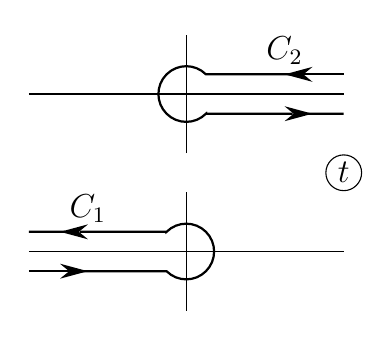
\begin{tikzpicture}
	\draw[-] (-2,1)--(2,1);
	\draw[-] (0,0.25)--(0,1.75);
	\draw[thick] (2, 1.25) [-{Stealth[length=10pt, angle'=30]}]-- (1.25, 1.25);
	\draw[thick] (1.35, 1.25) -- (0.25, 1.25) 
	arc[radius = 0.35355cm, start angle = 45, delta angle = 270]
	-- (0.25, 0.75) -- (1.35, 0.75)
	(1.25, 0.75) [{Stealth[length=10pt, angle'=30, reversed]}-]-- (2, 0.75);
	%\node[font=\large,above] at (0, 0) {$E_i$};
	\node[font=\large,above] at (1.25, 1.25) {$C_2$};
	%\fill (0, 0) circle(1.5pt);
	\draw[-] (-2,-1)--(2,-1);
	\draw[-] (0,-0.25)--(0,-1.75);
	\draw[thick] (-2, -1.25) [-{Stealth[length=10pt, angle'=30]}]-- (-1.25, -1.25);
	\draw[thick] (-1.35, -1.25) -- (-0.25, -1.25) 
	arc[radius = 0.35355cm, start angle = 225, delta angle = 270]
	-- (-0.25, -0.75) -- (-1.35, -0.75)
	(-1.25, -0.75) [{Stealth[length=10pt, angle'=30, reversed]}-]-- (-2, -0.75);
	\node[font=\large,above] at (-1.25, -0.75) {$C_1$};
	\node [font=\large] at (2,0) {$t$};
	\draw (2,0) circle (1.5ex);
	\end{tikzpicture}\caption{FIG. 52}\label{Fig.52}}
\parbox[]{.5\textwidth}{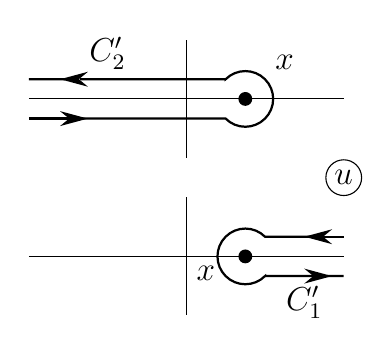
\begin{tikzpicture}
	\draw[-] (-2,1)--(2,1);
	\draw[-] (0,0.25)--(0,1.75);
	\draw[thick] (-2, 0.75) [-{Stealth[length=10pt, angle'=30]}]-- (-1.25, 0.75);
	\draw[thick] (-1.35, 0.75) -- (0.5, 0.75) 
	arc[radius = 0.35355cm, start angle = 225, delta angle = 270]
	-- (0.5, 1.25) -- (-1.35, 1.25)
	(-1.25,1.25) [{Stealth[length=10pt, angle'=30, reversed]}-]-- (-2, 1.25);
	\fill (0.75, 1) circle(2.5pt);
	%\node[font=\large,above] at (0, 0) {$E_i$};
	\node[font=\large,above] at (1.25, 1.25) {$x$};
	\node[font=\large,above] at (-1, 1.25) {$C_2'$};
	%\fill (0, 0) circle(1.5pt);
	\draw[-] (-2,-1)--(2,-1);
	\draw[-] (0,-0.25)--(0,-1.75);
	\draw[thick] (2, -0.75) [-{Stealth[length=10pt, angle'=30]}]-- (1.5, -0.75);
	\draw[thick] (1.75, -0.75) -- (1, -0.75) 
	arc[radius = 0.35355cm, start angle = 45, delta angle = 270]
	-- (1, -1.25) -- (1.75, -1.25)
	(1.5, -1.25) [{Stealth[length=10pt, angle'=30, reversed]}-]-- (2, -1.25);
	\node[font=\large,below] at (0.25, -1) {$x$};
	\node[font=\large,below] at (1.5, -1.25) {$C_1'$};
	\fill (0.75, -1) circle(2.5pt);
	\node [font=\large] at (2,0) {$u$};
	\draw (2,0) circle (1.5ex);
	\end{tikzpicture}\caption{FIG. 53}\label{Fig.53}}
\end{figure}







As $ x \to +\infty $, the whole path of integration $ C_1' $ moves to infinity, and the integral in \eqref{a.3} tends to zero as $ \e^{-x^2} $. As $ x \to-\infty $, however, the path of integration extends along the whole of the real axis, and the integral in \eqref{a.3} does not tend exponentially to zero, so that the function $ y (x) $ becomes infinite essentially as $ \e^{x^2} $ Similarly, it is easy to see that the integral \eqref{a.2} along the contour $ C_2 $ diverges exponentially as $ x \to+\infty $.

For positive integral $ n $ (including zero), on the other hand, the integrals along the straight parts of the path of integration cancel, and the two integrals \eqref{a.3}, along $ C_1' $ and $ C_2' $, reduce to an integral along a closed path round the point $ u = x $. Thus we have the solution
\[ y(x)=\e^{x^2}\oint\frac{\e^{-u^2}}{(u-x)^{n+1}}\d u, \]
which satisfies the conditions stated. According to Cauchy’s well-known formula for the derivatives of an analytic function,
\[ f^{(n)}(x)=\frac{n!}{2\pi\i}\oint\frac{f(t)}{(t-x)^{n+1}}\d t, \]
$ y (x) $ is, apart from a constant factor, an \textit{Hermite polynomial}:
\begin{equation}\label{a.4}
H_n(x)=(-1)^n\e^{x^2}\frac{\d^n}{{\d x}^n}\e^{-x^2}.
\end{equation}



The polynomial $ H_n $, expanded in decreasing powers of $ x $, has the open form
\begin{equation}\label{a.5}
H_n(x)=(2x)^n-\frac{n(n-1)}{1}(2x)^{n-2}+\frac{n(n-1)(n-2)(n-3)}{1\cdot2}(2x)^{n-4}-\dots
\end{equation}
It contains only powers of $ x $ which are of the same parity as $ n $. We may write out here the first few Hermite polynomials:
\begin{equation}\label{a.6}
H_0=1, H_1=2x, H_2=4x^2-2, H_3=8x^3-12x, H_4=16x^4-48x^2+12.
\end{equation}



To calculate the normalization integral, we replace $ \e^{-x} H_n $ by its expression in \eqref{a.4} and integrate $ n $ times by parts:
\[ \int_{-\infty}^{+\infty}\e^{-x^2}H_n^2(x)\d x=\int_{-\infty}^{+\infty}(-1)^nH_n(x)\frac{\d^n}{{\d x}^n}\e^{-x^2}\d x=\int_{-\infty}^{\infty}\e^{-x^2}\frac{\d^nH_n}{\d x^n}\d x. \]
But $\d^nH_n/{\d x}^n $ is a constant, $ 2^nn! $. Thus
\begin{equation}\label{a.7}
\int_{-\infty}^{+\infty}\e^{-x^2}H_n^2(x)\d x=2^nn!\sqrt{\pi}.
\end{equation}

\section{The Airy function}\label{The Airy function}
The equation
\begin{equation}\label{b.1}
y''-xy=0
\end{equation}
is of Laplace’s type (see \S\ref{Hermite polynomials}). Following the general method, we form the functions
\[ P=t^2,\quad Q=-1,\quad Z=-\exp(-t^3/3),\quad V=\exp(xt-t^3/3), \]
so that the solution can be represented in the form
\begin{equation}\label{b.2}
y(x)=\mathrm{const}\cdot\int_C\exp(xt-t^3/3)\d t,
\end{equation}
The path of integration $ C $ must be chosen so that the function $ V $ vanishes at both ends of it. These ends must therefore go to infinity in the regions of
\begin{wrapfigure}[]{l}[0cm]{0cm}
	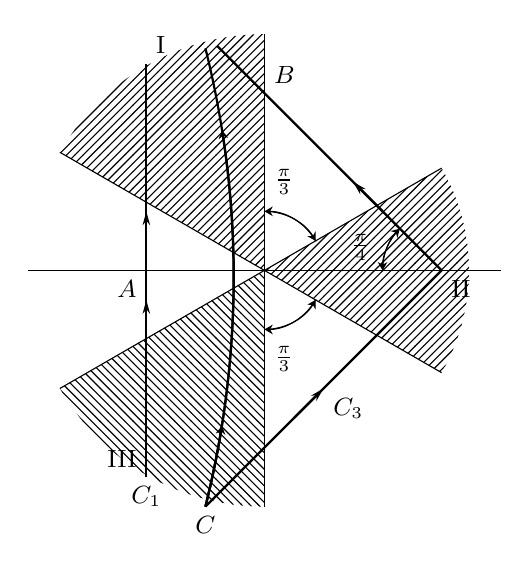
\begin{tikzpicture}[scale=1.5]
	\draw[-] (-2,0)--(2,0);
	\draw[-] (0,-2)--(0,2);
	\draw[ domain =-1.73205:1.5,smooth] plot(\x,{0.57735*\x});
	\draw[ domain =-1.73205:1.5,smooth] plot(\x,{-0.57735*\x});
	\fill[pattern=north west lines] (-1.73205,-1) -- (0,0) -- (0,-2) --(210:2) arc (210:270:2)-- cycle;
	\draw (0,-0.5)[-{Stealth[length=3pt, angle'=60]}]--(270:0.5) arc(270:330:0.5);
	\draw (0.433,-0.25)[-{Stealth[length=3pt, angle'=60]}]--(330:0.5) arc(330:270:0.5);
	\node[font=\small,right] at (0, -0.75) {$\frac{\pi}{3}$};
	\draw (0,0.5)[-{Stealth[length=3pt, angle'=60]}]--(90:0.5) arc(90:30:0.5);
	\draw (0.433,0.25)[-{Stealth[length=3pt, angle'=60]}]--(30:0.5) arc(30:90:0.5);
	\node[font=\small,right] at (0, 0.75) {$\frac{\pi}{3}$};
	\node[font=\small,below] at (-0.5,-2) {$ C $};
	\draw[thick] (-0.5,-2)[-{Stealth[length=5pt, angle'=30]}]--(0.5,-1);
	\draw[thick] (0.25,-1.25)--(1.5,0);
	\draw[thick] (1.5,0)[-{Stealth[length=5pt, angle'=30]}]--(0.75,0.75);
	\draw[thick] (1,0.5)--(-0.4,1.9);
	\draw (1,0)[-{Stealth[length=3pt, angle'=60]}]--(1,0)arc[radius = 0.5cm, start angle = 180, delta angle = -45];
	\draw (1.14645,0.35355)[-{Stealth[length=3pt, angle'=60]}]--(1.14645,0.35355)arc[radius = 0.5cm, start angle = 135, delta angle = 45];
	\node[font=\small,above right] at (0.65,0) {$ \frac{\pi}{4} $};
	\draw[thick,smooth] (-0.5,-2)[-{Stealth[length=3pt, angle'=60]}]--(-0.5,-2)arc[radius=8cm, start angle=345.9637,delta angle = 5];
	\draw[thick,smooth] (-0.5,-2)[-{Stealth[length=3pt, angle'=60]}]--(-0.5,-2)arc[radius=8cm, start angle=345.9637,delta angle = 23];
	\draw[thick,smooth] (-0.5,-2)--(-0.5,-2)arc[radius=8cm, start angle=345.9637,delta angle = 28.0725];
	\draw[thick] (-1,-1.75)[-{Stealth[length=5pt, angle'=30]}]--(-1,-0.25);
	\draw[thick] (-1,-0.5)[-{Stealth[length=5pt, angle'=30]}]--(-1,0.5);
	\draw[thick](-1,-0.25)--(-1,1.75);
	\fill[pattern=north east lines] (0,0) -- (1.5,-0.8660) --(330:1.7321) arc (-30:30:1.7321)-- cycle;
	\fill[pattern=north east lines] (0,0) -- (0,2) --(90:2) arc (90:150:2)-- cycle;
	\node [font=\small,below] at (-1,-1.75) {$ C_1 $};
	\node [font=\small,below right] at (0.5,-1) {$ C_3 $};
	\node [font=\small,below left] at (-1,0) {$ A $};
	\node [font=\small,above right] at (0,1.5) {$ B $};
	\node [font=\small,below right] at (1.5,0) {II};
	\node [font=\small,above right] at (-1,1.75) {I};
	\node [font=\small,above left] at (-1,-1.75) {III};
	\end{tikzpicture}\caption{FIG.54}\label{Fig.54}
\end{wrapfigure} 
the complex plane of $ t $ in which  $ \mathrm{Re}(t^3) > 0 $ (the shaded regions in Fig. \ref{Fig.54}).





A solution finite for all $ x $ is obtained by taking the path $ C $ as shown in the figure. It can be displaced in any manner provided that the ends of it go to infinity in the same two shaded sectors (I and III in Fig. \ref{Fig.54}). We notice that, by taking a path which lay in sectors III and II (say), we should obtain a solution which becomes infinite as $ x \to\infty $.

Deforming the path $ C $ so that it goes along the imaginary axis, we obtain the function \eqref{b.2} in the form (substituting $ t = \i u $)
\begin{equation}\label{b.3}
\Phi(x)=\frac{1}{\sqrt{x}}\int_{0}^{\infty}\cos\left(ux+\frac{u^3}{3} \right)\d u.
\end{equation}



The constant in \eqref{b.2} has been put equal to $ -\i/2\sqrt{\pi} $, and we have denoted the function thus obtained by $ \Phi(x) $; it is called the \textit{Airy function}.\footnote{We follow the definition proposed by V. A. Fok; see G. D. Yakovleva, \textit{Tablitsy funktsi\v{i} Eri\v{i}} (\textit{Tables of Airy Functions}), Nauka. Moscow, 1969. The function $ \Phi(x) $ is one of two defined by Fok, who denotes it by $ V (x) $. In the literature, another definition of the Airy function is also found, which differs from \eqref{b.3} by a constant factor: $ \mathrm{Ai}(x) = \Phi(x)/\sqrt{\pi} $.}

The asymptotic expression for $ \Phi(x) $ for large values of $ x $ is obtained by calculating the integral \eqref{b.2} by the saddle-point method. For $ x > 0 $, the exponent in the integrand has an extremum for $ t = \pm\sqrt{x}  $, and the “direction of steepest descent” of the integrand is parallel to the imaginary axis. Accordingly, to obtain the asymptotic expression for large positive $ x $, we expand the exponent in powers of $ t + \sqrt{x} $ and integrate along the line $ C_1 $ (Fig. \ref{Fig.54}, which is parallel to the imaginary axis; the distance $ OA = \sqrt{x} $. Making the substitution $ t = -\sqrt{x} + \i u $, we have
\[ \Phi(x)\approx\frac{1}{2\sqrt{\pi}}\int_{-\infty}^{+\infty}\exp\left(-\frac{2}{3}x^{3/2}-\sqrt{x}u^2 \right)\d u, \]
whence
\begin{equation}\label{b.4}
\Phi(x)\approx\frac{1}{2x^{1/4}}\exp\left(-\frac{2}{3}x^{3/2} \right).
\end{equation}
Thus, for large positive $ x $, the function $ \Phi(x) $ diminishes exponentially.

To obtain the asymptotic expression for large negative values of $ x $, we notice that, for $ x < 0 $, the exponent has an extremum for $ t = \i\sqrt{|x|} $ and $ t = -\i\sqrt{|x|} $, and the direction of steepest descent at these points is along lines at angles $ -\pi/4 $ and $ \pi/4 $ respectively to the real axis. Taking as the path of integration the broken line $ C_3 $ (the distance $ OB = \sqrt{|x|} $), we have, after some simple transformations,
\begin{equation}\label{b.5}
\Phi(x)=\frac{1}{|x|^{1/4}}\sin\left(\frac{2}{3}|x|^{3/2}+\frac{\pi}{4} \right).
\end{equation}
Thus, in the region of large negative $ x $, the function $ \Phi(x) $ is oscillatory. We may mention that the first (and highest) maximum of the function $ \Phi(x) $ is $ \Phi(−1.02) = 0.95 $.

The Airy function can be expressed in terms of Bessel functions of order $ 1/3 $. The equation \eqref{b.1}, as can easily be seen, has the solution
\[ \sqrt{x}Z_{1/3}\left(\frac{2}{3}x^{3/2} \right), \]
where $ Z_{1/3}(x) $ is any solution of Bessel’s equation of order $ 1/3 $. The solution which is the same as \eqref{b.3} is
\begin{equation}\label{b.6}
\begin{split}
\Phi(x)=\frac{\sqrt{\pi x}}{3}\left[I_{-1/3}\left(\frac{2}{3}x^{3/2}-I_{1/3}\left(\frac{2}{3}x^{3/2} \right) \right) \right]\equiv\sqrt{\frac{x}{3\pi}}K_{1/3}\left(\frac{2}{3}x^{3/2} \right)\text{ for }x>0,\\
\Phi(x)=\frac{\sqrt{\pi|x|}}{3}\left[J_{-1/3}\left(\frac{2}{3}|x|^{3/2} \right)+J_{1/3}\left(\frac{2}{3}|x|^{3/2} \right) \right]\text{ for }x<0,
\end{split}
\end{equation}
where
\[ I_\nu(x)=\i^{-\nu}J_\nu(\i x),\quad K_\nu(x)=\frac{\pi}{2\sin\nu\pi}\left[I_{-\nu}(x)-I_\nu(x) \right]. \]
Using the recurrence relations
\[ K_{\nu-1}(x)-K_{\nu+1}(x)=-\frac{2\nu}{x}K_\nu(x), \]
\[ 2K_\nu'(x)=-K_{\nu-1}(x)-K_{\nu+1}(x) \]
we easily find for the derivative of the Airy function
\begin{wrapfigure}[8]{l}[0cm]{0cm}
	\centering
	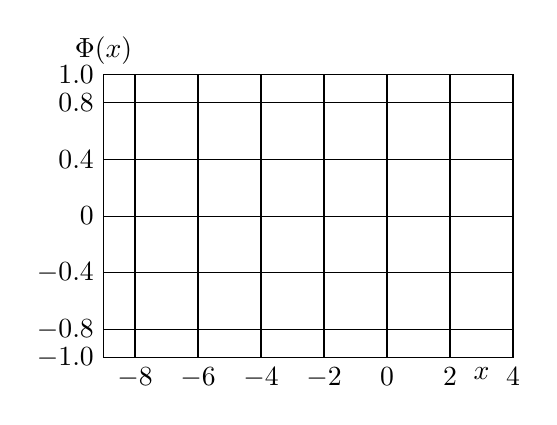
\begin{tikzpicture}[xscale=0.4,yscale=1.8]
	\draw (-9,-1)--(-9,1);
	\draw (-8,-1)--(-8,1);
	\draw (-6,-1)--(-6,1);
	\draw (-4,-1)--(-4,1);
	\draw (-2,-1)--(-2,1);
	\draw (0,-1)--(0,1);
	\draw (2,-1)--(2,1);
	\draw (4,-1)--(4,1);
	\draw (-9,-1)--(-9,1);
	\draw (-9,-1)--(4,-1);
	\draw (-9,-0.8)--(4,-0.8);
	\draw (-9,-0.4)--(4,-0.4);
	\draw (-9,0)--(4,0);
	\draw (-9,0.4)--(4,0.4);
	\draw (-9,0.8)--(4,0.8);
	\draw (-9,1)--(4,1);
	\draw plot[smooth] file{data};
	\node [below] at (-8,-1) {$ -8 $};
	\node [below] at (-6,-1) {$ -6 $};
	\node [below] at (-4,-1) {$ -4 $};
	\node [below] at (-2,-1) {$ -2 $};
	\node [below] at (0,-1) {$ 0 $};
	\node [below] at (2,-1) {$ 2 $};
	\node [below] at (4,-1) {$ 4 $};
	\node [left] at (-9,-1) {$ -1.0 $};
	\node [left] at (-9,-0.8) {$ -0.8 $};
	\node [left] at (-9,-0.4) {$ -0.4 $};
	\node [left] at (-9,0) {$ 0 $};
	\node [left] at (-9,0.4) {$ 0.4 $};
	\node [left] at (-9,0.8) {$ 0.8 $};
	\node [left] at (-9,1) {$ 1.0 $};
	\node [above] at (-9,1) {$ \Phi(x) $};
	\node [below] at (3,-1) {$ x $};
	\end{tikzpicture}\caption{FIG.55}\label{Fig.55}
\end{wrapfigure}
\begin{multline}\label{b.7}
\Phi'(x)=-\frac{x}{\sqrt{3\pi}}K_{2/3}\left(\frac{2}{3}x^{3/2} \right)\\
\text{ for }x>0.
\end{multline}


When $ x = 0 $,
\begin{equation}\label{b.8}
\begin{split}
\Phi(0)=\frac{\sqrt{\pi}}{3^{2/3}\Gamma(2/3)}=0.629,\\
\Phi'(0)=\frac{3^{1/6}\Gamma(2/3)}{2\sqrt{\pi}}=-0.459.
\end{split}
\end{equation}
Figure. \ref{Fig.55} shows a graph of the Airy function.



\section{Legendre polynomials\footnote{There are in the mathematical literature many good accounts of the theory of spherical harmonics. Here we shall give, for reference, only a few basic relations, and make no attempt at a systematic discussion of the theory of these functions.}}\label{Legendre polynomials}
The \textit{Legendre polynomials} $ P_l(\cos \theta) $ are defined by the formula
\begin{equation}\label{c.1}
P_l(\cos\theta)=\frac{1}{2^ll!}\frac{d^l}{(d\cos\theta)^l}(\cos^2\theta-1)^l.
\end{equation}



They satisfy the differential equation
\begin{equation}\label{c.2}
\frac{1}{\sin\theta}\frac{\d}{\d\theta}\left(\sin\theta\frac{\d P_l}{\d\theta} \right)+l(l+1)P_l=0.
\end{equation}
The associated Legendre polynomials are defined by
\begin{equation}\label{c.3}
P_l^m(\cos\theta)=\sin^m\theta\frac{\d^mP_l(\cos\theta)}{(\d\cos\theta)^m}=\frac{1}{2^ll!}\sin^m\theta\frac{\d^{l+m}}{(\d\cos\theta)^{l+m}}(\cos^2\theta-1)^l
\end{equation}
or, equivalently,
\begin{equation}\label{c.4}
P_l^m(\cos\theta)=(-1)^m\frac{(l+m)!}{(l-m)!2^ll!}\sin^{-m}\theta\frac{\d^{l-m}}{(\d\cos\theta)^{l-m}}(\cos^2\theta-1)^l,
\end{equation}
with $ m = 0, 1, \dots, l $. The associated polynomials satisfy the equation
\begin{equation}\label{c.5}
\frac{1}{\sin\theta}\frac{\d}{\d\theta}\left(\sin\theta\frac{\d P_l^m}{\d\theta} \right)+\left[l(l+1)-\frac{m^2}{\sin^2\theta} \right]P_l^m=0.
\end{equation}



The normalization integral $ \int_{-1}^{1}\left[P_l(\mu) \right]^2\d\mu (\mu=\cos \theta)$ for the Legendre polynomials is calculated by substituting \eqref{c.1} and integrating $ l $ times by parts, which gives
\[ \frac{(-1)^l}{2^{2l}(l!)^2}\int_{-1}^{1}(\mu^2-1)^l\frac{\d^{2l}}{{\d\mu}^{2l}}(\mu^2-1)^l\d\mu=\frac{(2l)!}{2^{2l}(l!)^2}\int_{-1}^{1}(1-\mu^2)^l\d\mu. \]
Substitution of $ u = (1 − \mu)/2 $ reduces this integral to Euler’s beta function, and the result is
\begin{equation}\label{c.6}
\int_{-1}^{1}[P_l(\mu)]^2\d\mu=\frac{2}{2l+1}.
\end{equation}
Similarly, it is easily seen that the functions $ P_l(\mu) $ with different $ l $ are orthogonal:
\begin{equation}\label{c.7}
\int_{-1}^{1}P_l(\mu)P_{l'}(\mu)\d\mu=0,l\ne l'.
\end{equation}



The calculation of the normalization integral for the associated Legendre polynomials is easily effected by a similar method. We write $ [P_l^m(\mu)]^2 $ as a product of the expressions \eqref{c.3} and \eqref{c.4}, and integrate $ l − m $ times by parts; the result is
\begin{equation}\label{c.8}
\int_{-1}^{1}[P_l^m(\mu)]^2\d\mu=\frac{2}{2l+1}\frac{(l+m)!}{(l-m)!}.
\end{equation}
It is also easily seen that the functions $ P_l^m $ with different $ l $ (and the same $ m $) are orthogonal:
\begin{equation}\label{c.9}
\int_{-1}^{1}P_l^m(\mu)P_{l'}^m(\mu)\d\mu=0,l\ne l'.
\end{equation}



The calculation of the integrals of products of three Legendre polynomials is discussed in \S107.

The following \textit{addition theorem} holds for Legendre polynomials. Let $\gamma$ be the angle between two directions defined by the spherical angles $ \theta, \phi $ and $ \theta', \phi': \cos \gamma = \cos \theta \cos \theta' + \sin \theta \sin \theta' \cos (\phi - \phi')$. Then
\begin{multline}\label{c.10}
P_l(\cos\gamma)=P_l(\cos\theta)P_l(\cos\theta')+\\
+\sum_{m-1}^{l}2\frac{(l-m)!}{(l+m)!}P_l^m(\cos\theta)P_l^m(\cos\theta')\cos[m(\phi-\phi')].
\end{multline}
This theorem can also be written in terms of the spherical harmonic functions defined by \eqref{28.7}:
\begin{equation}\label{c.11}
P_l(\bm{nn'})=\frac{4\pi}{2l+1}\sum_{m=-1}^l Y_{lm}^*(\bm{n'})Y_{lm}(\bm{n}).
\end{equation}



Here $ \bm{n} $ and $ \bm{n'} $ are two unit vectors, and $ Y_{lm}(\bm{n}) $ denotes the spherical harmonic function of the polar angle and azimuth of the direction of $ \bm{n} $ relative to a fixed system of coordinates.

If equation \eqref{c.10} is multiplied by $ P_{l'}(\cos \theta) $ and integrated over $ \d o = \sin \theta \d\theta \d\phi $, the integration with respect to $\phi$ gives zero for all terms on the right that contain factors $ \cos [m (\phi-  \phi')] $; using \eqref{c.6} and \eqref{c.7}, we obtain
\[ \int P_l(\cos\gamma)P_{l'}(\cos\theta)\d o=\delta_{ll'}\frac{4\pi}{2l+1}P_l(\cos\theta') .\]
This result may be written in the symmetrical form
\begin{equation}\label{c.12}
\int P_l(\bm{n}_1\bm{n}_2)P_{l'}(\bm{n_1}\bm{n_3})\d o_1=\delta_{ll'}\frac{4\pi}{2l+1}P_l(\bm{n}_2\bm{n}_3),
\end{equation}



where $ \bm{n}_1 , \bm{n}_2, \bm{n}_3$ are three unit vectors and the integration is with respect to the direction of $ \bm{n}_1 $.

Finally, we give the first few normalized spherical harmonics $ Y_{lm} $:
\[ Y_{00}=\frac{1}{\sqrt{4\pi}},\quad Y_{10}=\i\sqrt{\frac{3}{4\pi}}\cos\theta,\quad Y_{1,\pm1}=\pm\i\sqrt{\frac{3}{8\pi}}\sin\theta\cdot\e^{\pm\i\phi}, \]
\[ Y_{20}=\sqrt{\frac{5}{16\pi}}(1-3\cos^2\theta),\quad Y_{2,\pm1}=\pm\sqrt{\frac{15}{8\pi}}\cos\theta\sin\theta\cdot\e^{+\i\phi}, \]
\[ Y_{2,\pm2}=-\sqrt{\frac{15}{32\pi}}\sin^2\theta\cdot\e^{\pm2\i\phi},\quad Y_{30}=-\i\sqrt{\frac{7}{16\pi}}\cos\theta(5\cos^2\theta-3), \]
\[ Y_{3,\pm1}=\pm\i\sqrt{\frac{21}{64\pi}}\sin\theta(5\cos^2\theta-1)\e^{\pm\i\phi}, \]
\[ Y_{3,\pm2}=-\i\sqrt{\frac{105}{32\pi}}\cos\theta\sin^2\theta\cdot\e^{\pm2\i\phi},\quad Y_{3,\pm3}=\pm\i\sqrt{\frac{35}{64\pi}}\sin^3\theta\cdot\e^{\pm3\i\phi}. \]
\section{The confluent hypergeometric function}\label{The confluent hypergeometric function}
The \textit{confluent hypergeometric function} is defined by the series
\begin{equation}\label{d.1}
F(\alpha,\gamma,z)=1+\frac{\alpha}{\gamma}\frac{z}{1!}+\frac{\alpha(\alpha+1)}{\gamma(\gamma+1)}\frac{z^2}{2!}+\dots,
\end{equation}
which converges for all finite $ z $; the parameter $\alpha$ is arbitrary, while the parameter $\gamma$ is supposed not zero or a negative integer. If $\alpha$ is a negative integer (or zero), $ F (\alpha, \gamma, z) $ reduces to a polynomial of degree $ |\alpha| $.

The function $ F (\alpha, \gamma, z) $ satisfies the differential equation
\begin{equation}\label{d.2}
zu''+(\gamma-z)u'-\alpha u=0,
\end{equation}
as is easily seen by direct verification.\footnote{The equation \eqref{d.2} with a negative integral $\gamma$ does not require special discussion, since it can be reduced to a case of positive integral $\gamma$ by the transformation which gives equation \eqref{d.3}.
} By the substitution $ u = z^{1-\gamma} u_1 $, this equation is transformed into another of the same form,
\begin{equation}\label{d.3}
zu_1''+(2-\gamma-z)u_1'-(\alpha-\gamma+1)u_1=0.
\end{equation}
Hence we see that, for non-integral $\gamma$, equation \eqref{d.2} has also the particular integral $ z^{1-\gamma}F (\alpha-\gamma+1, 2-\gamma, z) $, which is linearly independent of \eqref{d.1}, so that the general solution of equation \eqref{d.2} is of the form
\begin{equation}\label{d.4}
u=c_1F(\alpha,\gamma,z)+c_2z^{1-\gamma}F(\alpha-\gamma+1,2-\gamma,z).
\end{equation}
The second term, unlike the first, has a singular point at $ z = 0 $.

Equation \eqref{d.2} is of Laplace’s type, and its solutions can be represented as contour integrals. Following the general method, we form the functions
\[ P(t)=\gamma t-\alpha,\quad Q(t)=t(t-1),\quad Z(t)=t^{\alpha-1}(t-1)^{\gamma-\alpha-1}, \]
so that
\begin{equation}\label{d.5}
u=\int\e^{tz}t^{\alpha-1}(t-1)^{\gamma-\alpha-1}\d t.
\end{equation}
The path of integration must be chosen so that the function $ V(t) = \e^{tz}t^\alpha (t - 1)^{\gamma-\alpha} $ returns to its original value on traversing the path. Applying the same method to equation \eqref{d.3}, we can obtain for u a contour integral of another form:
\[ u=z^{1-\gamma}\int\e^{tz}t^{\alpha-\gamma}(t-1)^{-\alpha}\d t. \]
The substitution $ tz \to t $ reduces this integral to the convenient form
\begin{equation}\label{d.6}
u(z)=\int\e^t(t-z)^{-\alpha}t^{\alpha-\gamma}\d t,
\end{equation}
and the corresponding function $ V $ to
\[ V(t)=\e^t(t-z)^{-\alpha}t^{\alpha-\gamma}\d t, \]



The integrand in \eqref{d.6} has in general two singular points, at $ t = z $ and $ t = 0 $. We take a contour of integration $ C $ which passes from infinity ($ \text{Re}t \to-\infty $)
\begin{wrapfigure}[]{l}[0cm]{0cm}
	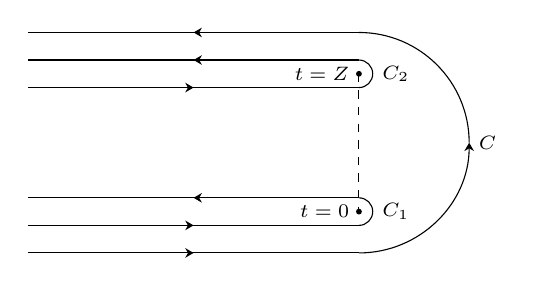
\begin{tikzpicture}[scale=0.7]
	\draw (-6,-2)[-{Stealth[length=3pt, angle'=60]}]--(-3,-2);
	\draw (-4,-2)--(0,-2);
	\draw (0,-2)[-{Stealth[length=3pt, angle'=60]}]--(0,-2)arc[radius = 2cm, start angle = -90, delta angle = 90];
	\draw (2,0)--(2,0)arc[radius = 2cm, start angle = 0, delta angle = 90];
	\draw (0,2)[-{Stealth[length=3pt, angle'=60]}]--(-3,2);
	\draw (-2,2)--(-6,2);
	
	\draw (-6,-1.5)[-{Stealth[length=3pt, angle'=60]}]--(-3,-1.5);
	\draw (-4,-1.5)--(0,-1.5);
	\draw (0,-1.5)arc[radius = 0.25cm, start angle = -90, delta angle = 180];
	\draw (0,-1)[-{Stealth[length=3pt, angle'=60]}]--(-3,-1);
	\draw (-2,-1)--(-6,-1);
	
	\draw (-6,1)[-{Stealth[length=3pt, angle'=60]}]--(-3,1);
	\draw (-4,1)--(0,1);
	\draw (0,1)arc[radius = 0.25cm, start angle = -90, delta angle = 180];
	\draw (0,1.5)[-{Stealth[length=3pt, angle'=60]}]--(-3,1.5);
	\draw (-2,1.5)--(-6,1.5);
	\fill (0,-1.25) circle(1.5pt);
	\node [left,font=\scriptsize] at (0,-1.25) {$ t=0 $};
	\fill (0,1.25) circle(1.5pt);
	\node [left,font=\scriptsize] at (0,1.25) {$ t=Z $};
	\draw[dashed] (0,1.25)--(0,-1.25);
	\node[right,font=\scriptsize] at (0.25,-1.25) {$ C_1 $};
	\node[right,font=\scriptsize] at (0.25,1.25) {$ C_2 $};
	\node[right,font=\scriptsize] at (2,0) {$ C $};
	\end{tikzpicture}\caption{FIG. 56}\label{Fig.56}
\end{wrapfigure}
round the two singular points in the positive direction and back to infinity (Fig. \ref{Fig.56}). This contour satisfies the required conditions, since $ V (t) $ vanishes at its ends. The integral \eqref{d.6}, taken along the contour $ C $, has no singular point for $ z = 0 $; hence it must be the same, apart from a constant factor, as the function $ F (\alpha, \gamma, z) $, which also has no singularity. For $ z = 0 $ the two singular points of the integrand coincide; according to a well-known formula in the theory of the gamma function,
\begin{equation}\label{d.7}
\frac{1}{2\pi\i}\int_C\e^tt^{-\gamma}\d t=\frac{1}{\Gamma(\gamma)}.
\end{equation}
Since $ F (\alpha, \gamma, 0)=1 $, it is evident that
\begin{equation}\label{d.8}
F (\alpha, \gamma, z) =\frac{\Gamma(\gamma)}{2\pi\i}\int_C\e^t(t-z)^{-\alpha}t^{\alpha-\gamma}\d t.
\end{equation}
The integrand in \eqref{d.5} has singular points at $ t = 0 $ and $ t = 1 $.
\begin{wrapfigure}[6]{r}[0cm]{0cm}
	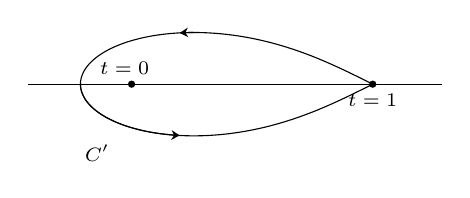
\begin{tikzpicture}[xscale=1.75,yscale=0.875]
	\draw [-{Stealth[length=3pt, angle'=60]}][domain=-45:-28,scale=1.5,samples=500] plot (\x:{-(2* cos(2*\x))^0.5});
	\draw [-{Stealth[length=3pt, angle'=60]}][domain=-30:28,scale=1.5,samples=500] plot (\x:{-(2* cos(2*\x))^0.5});
	\draw [domain=0:45,scale=1.5,samples=500] plot (\x:{-(2* cos(2*\x))^0.5});
	\draw[-] (-2.5,0)--(0.5,0);
	\fill[xscale=0.5] (-3.5,0) circle(1.5pt);
	\node[font=\scriptsize,above] at (-1.8,0) {$ t=0 $}; 
	\fill[xscale=0.5] (0,0) circle(1.5pt);
	\node[font=\scriptsize,below] at (0,0) {$ t=1 $}; 
	\node[font=\scriptsize] at (-2,-1) {$ C' $}; 
	\end{tikzpicture}\caption{FIG. 57}\label{Fig.57}
\end{wrapfigure} 
If $ \mathrm{Re}(\gamma-\alpha) > 0 $,
and $\gamma$ is not a positive integer, the path of integration can be taken as a contour $ C' $ starting from the point $ t = 1 $, passing round the point $ t = 0 $ in the positive direction, and returning to $ t = 1 $ (Fig. \ref{Fig.57}); for $ \mathrm{Re}(\gamma-\alpha) > 0 $, the function $ V (t) $ returns to its original value of zero on passing round such a contour.\footnote{If $\gamma$ is a positive integer, $ C' $ can be any contour which passes round both the points $ t = 0 $ and $ t = 1 $} The integral thus defined again has no singularity for $ z = 0 $, and is related to $ F (\alpha, \gamma, z) $ by
\begin{equation}\label{d.9}
F(\alpha, \gamma, z)=-\frac{1}{2\pi\i}\frac{\Gamma(1-\alpha)\Gamma(\gamma)}{\Gamma(\gamma-\alpha)}\oint_{C'}\e^{tz}(-t)^{\alpha-1}(1-t)^{\gamma-\alpha-1}\d t.
\end{equation}





The following remark should be made concerning the integrals \eqref{d.8}, \eqref{d.9}. For non-integral $\alpha$ and $\gamma$, the integrands are not one-valued functions. Their values at each point are supposed chosen in accordance with the condition that the complex quantity which is raised to a power is taken with the argument whose absolute value is least.

We may notice the useful relation
\begin{equation}\label{d.10}
F(\alpha,\gamma,z)=\e^zF(\gamma-\alpha,\gamma,-z),
\end{equation}
which is obtained at once by substituting $ t \to t + z $ in the integral \eqref{d.8}.

We have already remarked that, if $ \alpha = -n $, where $ n $ is a positive integer, the function $ F (\alpha, \gamma, z) $ reduces to a polynomial. A concise formula can be obtained for these polynomials. Making in the integral \eqref{d.9} the substitution $ t \to 1-(t/z) $ and applying Cauchy’s formula to the resulting integral, we find
\begin{equation}\label{d.11}
F(-n,\gamma,z)=\frac{1}{\gamma(\gamma+1)\dots(\gamma+n-1)}z^{1-\gamma}\e^z\frac{\d^m}{{\d z}^n}(\e^{-z}z^{\gamma+n-1}).
\end{equation}
If also $ \gamma = $ a positive integer $ m $, we have the formula
\begin{equation}\label{d.12}
F(-n,m,z)=\frac{(-1)^{m-1}}{m(m+1)\dots(m+n-1)}\e^z\frac{\d^{m+n-1}}{{\d z}^{m+n-1}}(\e^{-z}z^n).
\end{equation}
This formula is obtained by applying Cauchy’s formula to the integral derived from \eqref{d.8} by the substitution $ t \to z - t $.

The polynomials $ F (-n, m, z), 0 \leqslant m \leqslant n $, are (apart from a constant factor) the \textit{generalized Laguerre polynomials}
\begin{multline}\label{d.13}
L_n^m(z)=(-1)^m\frac{(n!)^2}{m!(n-m)!}F(-(n-m),m+1,z)=\\
=\frac{n!}{(n-m)!}\e^z\frac{\d^n}{{\d z}^n}\e^{-z}z^{n-m}=(-1)^m\frac{n!}{(n-m)!}\e^zz^{-m}\frac{\d^{n-m}}{{\d z}^{n-m}}\e^{-z}z^n.
\end{multline}
The polynomials $ L_n^m $ for $ m = 0 $ are denoted by $ L_n(z) $ and are called simply \textit{Laguerre polynomials}; from \eqref{d.13} we have
\[ L_n)z =\e^z\frac{\d^n}{{\d z}^n}(\e^{-z}z^n). \]



The integral representation \eqref{d.8} is convenient for obtaining the asymptotic expansion of the confluent hypergeometric function for large $ z $. We deform the contour into two contours $ C_1 $ and $ C_2 $ (Fig. 56), which pass round the points $ t = 0 $ and $ t = z $ respectively; the lower branch of $ C_2 $ and the upper branch of $ C_1 $ are supposed to join at infinity. To obtain an expansion in inverse powers of $ z $, we take $ (-z)^{-\alpha} $ outside the parenthesis in the integrand. In the integral along the contour $ C_2 $, we make the substitution $ t \to t + z $; the contour $ C_2 $ is thereby transformed into $ C_1 $ We thus represent the formula \eqref{d.8} as
\begin{multline}\label{d.14}
F(\alpha,\gamma,z)=\frac{\Gamma(\gamma)}{\Gamma(\gamma-\alpha)}(-z)^{-\alpha}G(\alpha,\alpha-\gamma+1,-z)+\\
+\frac{\Gamma(\gamma)}{\Gamma(\alpha)}\e^z z^{\alpha-\gamma}G(\gamma-\alpha,1-\alpha,z),
\end{multline}
where
\begin{equation}\label{d.15}
G(\alpha,\beta,z)=\frac{\Gamma(1-\beta)}{2\pi\i}\int_{C_1}\left(1+\frac{t}{z} \right)^{-\alpha}t^{\beta-1}\e^t\d t.
\end{equation}
In raising $ -z $ and $ z $ to powers in the formula \eqref{d.14} we must take the arguments which have the smallest absolute value. Finally, expanding $ (1 + t/z)^{-\alpha} $ in the integrand in powers of $ t/z $ and applying formula \eqref{d.7}, we have for $ G (\alpha, \beta, z) $ the asymptotic series
\begin{equation}\label{d.16}
G(\alpha,\beta,z)=1+\frac{\alpha\beta}{1!z}+\frac{\alpha(\alpha+1)\beta(\beta+1)}{2!z^2}+\dots
\end{equation}
Formulae \eqref{d.14} and \eqref{d.16} give the asymptotic expansion of the function $ F (\alpha, \gamma, z) $.

For positive integral $\gamma$, the second term in the general solution \eqref{d.4} of equation \eqref{d.2} is either the same as the first term (if $ \gamma = 1 $) or meaningless (if $ \gamma > 1 $). In this case we can take, as a set of two linearly independent solutions, the two terms in formula \eqref{d.14}, i.e. the integrals \eqref{d.8} taken along the contours $ C_1 $ and $ C_2 $ (these contours, like $ C $, satisfy the required conditions, so that the integrals along them are solutions of equation \eqref{d.2}). The asymptotic form of these solutions is given by the formulae already obtained; it remains for us to find their expansion in ascending powers of $ z $. To do this, we start from equation \eqref{d.14} and the analogous equation for the function $ z^{1-\gamma} F (\alpha-\gamma + 1, 2 -\gamma, z) $. From these two equations we express $ G (\alpha, \alpha-\gamma  + 1, - z) $ in terms of $ F (\alpha, \gamma, z) $ and $ F (\alpha-\gamma  + 1, 2 -\gamma, z) $; we then put $ \gamma= p + \epsilon  $($ p $ being a positive integer), and pass to the limit $ \epsilon\to0 $, resolving the indeterminacy by L’Hospital’s rule. A fairly lengthy calculation gives the following expansion:
\begin{multline}\label{d.17}
G(\alpha,\alpha-p+1,-z)=\frac{\sin\pi\alpha\cdot\Gamma(p-a)}{\pi\Gamma(p)}z^\alpha\times\\
\times\left\{\ln z\cdot F(\alpha,p,z)
+\sum_{s=0}^\infty\frac{\Gamma(p)\Gamma(\alpha+s)\left[\psi(\alpha+s)-\psi(p+s)-\psi(s+1) \right]}{\Gamma(\alpha)\Gamma(s+p)\Gamma(s+1)}z^s+\right.\\
\left.+\sum_{s=1}^{p-1}(-1)^{s+1}\frac{\Gamma(s)\Gamma(\alpha-s)\Gamma(p)}{\Gamma(\alpha)\Gamma(p-s)}z^{-s}    \right\},
\end{multline}
where $\psi$ denotes the logarithmic derivative of the gamma function: $ \psi(\alpha = \Gamma'(\alpha)/\Gamma(\alpha) $.
\section{The hypergeometric function}\label{The hypergeometric function}
The \textit{hypergeometric function} is defined in the circle $ |z| < 1 $ by the series
\begin{equation}\label{e.1}
F(\alpha,\beta,\gamma,z)=1+\frac{\alpha\beta}{\gamma}\frac{z}{1!}+\frac{\alpha(\alpha+1)\beta(\beta+1)}{\gamma(\gamma+1)}\frac{z^2}{2!}+\dots,
\end{equation}
and for $ |z| > 1 $ it is obtained by analytical continuation of this series (see \eqref{e.6}). The hypergeometric function is a particular integral of the differential equation
\begin{equation}\label{e.2}
z(1-z)u''+[\gamma-(\alpha+\beta+1)z]u'-\alpha\beta u=0.
\end{equation}
The parameters $\alpha$ and $\beta$ are arbitrary, while $ γ \ne 0, -1, -2, \dots $ The function $ F (\alpha, \beta, \gamma, z) $ is evidently symmetrical with respect to the parameters $\alpha$ and $\beta$.\footnote{The confluent hypergeometric function is obtained from $ F (\alpha, \beta, \gamma, z) $ by taking the limit
\[ F (\alpha, \gamma, z)=\lim\limits_{\beta\to\infty}F (\alpha, \beta, \gamma, \frac{z}{\beta}) \]
	
	
	
The notation$ {}_2F_1(\alpha, \beta, \gamma, z) $ for the hypergeometric function and $ {}_1F_1(\alpha, \gamma, z) $ for the confluent hypergeometric function is also used in the literature. The subscripts to the left and right of $ F $ show the numbers of parameters in the numerators and denominators respectively of the terms in the series.
} The second independent solution of equation \eqref{e.2} is
\[ z^{1-\gamma}F(\beta-\gamma+1,\alpha-\gamma+1,2-\gamma,z); \]
it has a singular point at $ z = 0 $.

We shall give here for reference a number of relations obeyed by the hypergeometric function.

The function $ F (\alpha, \beta, \gamma, z) $ can be represented for all $ z $, if $ \mathrm{Re}(γ − α) > 0 $, as an integral:
\begin{multline}\label{e.3}
F(\alpha,\beta,\gamma,z)=\\
=-\frac{1}{2\pi\i}\frac{\Gamma(1-\alpha)\Gamma(\gamma)}{\Gamma(\gamma-\alpha)}\oint_{C'}(-t)^{\alpha-1}(1-t)^{\gamma-\alpha-1}(1-tz)^{-\beta}\d t,
\end{multline}
taken along the contour $ C' $ shown in Fig. \ref{Fig.57}. That this integral in fact satisfies equation \eqref{e.2} is easily seen by direct substitution; the constant factor is chosen so as to give unity for $ z = 0 $.

The substitution $ u = (1 - z)^{\gamma-\alpha-\beta}u_1 $ in equation \eqref{e.2} leads to an equation of the same form, with parameters $ \gamma-\alpha, \gamma-\beta, \gamma $ in place of $ \alpha, \beta, \gamma $ respectively. Hence we have
\begin{equation}\label{e.4}
F(\alpha,\beta,\gamma,z)=(1-z)^{\gamma-\alpha-\beta}F(\gamma-\alpha,\gamma-\beta,\gamma,z)
\end{equation}
both sides of this equation satisfy the same equation, and they have the same value for $ z = 0 $.

The substitution $ t \to t/(1 - z + zt) $ in the integral \eqref{e.3} leads to the following relation between hypergeometric functions with variables $ z $ and $ z/(z − 1) $:
\begin{equation}\label{e.5}
F(\alpha,\beta,\gamma,z)=(1-z)^{-\alpha}F\left(\alpha,\gamma-\beta,\gamma,\frac{z}{z-1}\right).
\end{equation}
The value of the many-valued expression $ (1 - z)^{-\alpha} $ in this formula (and of similar expressions in all the following formulae) is determined by the condition that the complex quantity which is raised to a power is taken with the argument whose absolute value is least.

Next we shall give, without proof, an important formula relating hypergeometric functions with variables $ z $ and $ 1/z $:
\begin{multline}\label{e.6}
F(\alpha,\beta,\gamma,z)=\frac{\Gamma(\gamma)\Gamma(\beta-\alpha)}{\Gamma(\beta)\Gamma(\gamma-\alpha)}(-z)^{-\alpha}F\left(\alpha,\alpha+1-\gamma,\alpha+1-\beta,\frac{1}{z}\right)+\\
+\frac{\Gamma(\gamma)\Gamma(\alpha-\beta)}{\Gamma(\alpha)\Gamma(\gamma-\beta)}(-z)^{-\beta}F\left(\beta,\beta+1-\gamma,\beta+1-\alpha,\frac{1}{z} \right).
\end{multline}
This formula expresses $ F (\alpha, \beta, \gamma, z) $ as a series which converges for $ |z| > 1 $, i.e. it is the analytical continuation of the original series \eqref{e.1}.

The formula
\begin{multline}\label{e.7}
F(\alpha,\beta,\gamma,z)=\frac{\Gamma(\gamma)\Gamma(\gamma-\alpha-\beta)}{\Gamma(\gamma-\alpha)\Gamma(\gamma-\beta)}F(\alpha,\beta,\alpha+\beta+1-\gamma,1-z)+\\
+\frac{\Gamma(\gamma)\Gamma(\alpha+\beta-\gamma)}{\Gamma(\alpha)\Gamma(\beta)}(1-z)^{\gamma-\alpha-\beta}F(\gamma-\alpha,\gamma-\beta,\gamma+1-\alpha-\beta,1-z).
\end{multline}
relates hypergeometric functions of $ z $ and $ 1 - z $; again, the proof will not be given here. Combining \eqref{e.7} with \eqref{e.6}, we obtain the relations
\begin{multline}\label{e.8}
F(\alpha,\beta,\gamma,z)=\frac{\Gamma(\gamma)\Gamma(\beta-\alpha)}{\Gamma(\beta)\Gamma(\gamma-\alpha)}(1-z)^{-\alpha}F\left(\alpha,\gamma-\beta,\alpha+1-\beta,\frac{1}{1-z} \right)+\\
+\frac{\Gamma(\gamma)\Gamma(\alpha-\beta)}{\Gamma(\alpha)\Gamma(\gamma-\beta)}(1-z)^{-\beta}F(\beta,\gamma-\alpha,\beta+1-\alpha,\frac{1}{1-z}),
\end{multline}
\begin{multline}\label{e.9}
F(\alpha,\beta,\gamma,z)=\frac{\Gamma(\gamma)\Gamma(\gamma-\alpha-\beta)}{\Gamma(\gamma-\beta)\Gamma(\gamma-\alpha)}\times\\
\times z^{-\alpha}F\left(\alpha,\alpha+1-\gamma,\alpha+\beta+1-\gamma,\frac{z-1}{z} \right)+\frac{\Gamma(\gamma)\Gamma(\alpha+\beta-\gamma)}{\Gamma(\alpha)\Gamma(\beta)}\times\\
\times(1-z)^{\gamma-\alpha-\beta}z^{\beta-\gamma}F\left(1-\beta,\gamma-\beta,\gamma+1-\alpha-\beta,\frac{z-1}{z} \right).
\end{multline}
Each of the terms in the sums on the right of equations \eqref{e.6}--\eqref{e.9} is itself a solution of the hypergeometric equation.

If $\alpha$ (or $\beta$) is a negative integer or zero, $ \alpha = -n $, the hypergeometric function reduces to a polynomial of the $ n $th degree, and can be represented in the form
\begin{equation}\label{e.10}
F(-n,\beta,\gamma,z)=\frac{z^{1-\gamma}(1-z)^{\gamma+n-\beta}}{\gamma(\gamma+1)\dots(\gamma+n-1)}\frac{\d^n}{{\d z}^n}\left[z^{\gamma+n-1}(1-z)^{\beta-\gamma} \right].
\end{equation}
These polynomials are the same, apart from a constant factor, as the \textit{Jacobi polynomials}, defined by
\begin{multline}\label{e.11}
P_n^{(a,b)}(z)=\frac{(a+1)(a+2)\dots(a+n)}{n!}F\left(-n,a+b+n+1,a+1,\frac{1-z}{2} \right)=\\
=\frac{(-1)^n}{2^n n!}(1-z)^{-a}(1+z)^{-b}\frac{\d^n}{{\d z}^n}\left[(1-z)^{a+n}(1+z)^{b+n} \right].
\end{multline}
For $ a = b = 0 $, the Jacobi polynomials are the Legendre polynomials. For $ n = 0 $, $ P_0^{(a, b)} = 1 $.




\section{The calculation of integrals containing confluent hypergeometric functions}\label{The calculation of integrals containing confluent hypergeometric functions}
Let us consider an integral of the form
\begin{equation}\label{f.1}
J_{\alpha\gamma}^\nu=\int_{0}^{\infty}\e^{-\lambda z}z^\nu F(\alpha,\gamma,kz)\d z.
\end{equation}
We assume that it converges. If this is so we must have $ \mathrm{Re} \nu > -1 $ and $ \mathrm{Re}\lambda >| \mathrm{Re} k| $; if $\alpha$ is a negative integer, the latter condition can be replaced by $ \mathrm{Re}\lambda >0$. Using for $ F (\alpha, \gamma, kz) $ the integral representation \eqref{d.9} and effecting the integration over $ z $ under the contour integral, we have
\begin{multline*}
J_{\alpha\gamma}^\nu=-\frac{1}{2\pi\i}\frac{\Gamma(1-\alpha)\Gamma(\gamma)}{\Gamma(\gamma-\alpha)}\lambda^{-\nu-1}\Gamma(\nu+1)\times\\
\times\oint_{C'}(-t)^{\alpha-1}(1-t)^{\gamma-\alpha-1}(1-(k/\lambda)t)^{-\nu-1}\d t.
\end{multline*}



Using \eqref{e.3}, we have finally
\begin{equation}\label{f.2}
J_{\alpha\gamma}^\nu=\Gamma(\nu+1)\lambda^{-\nu-1}F(\alpha,\nu+1,\gamma,k/\lambda).
\end{equation}
In the cases where the function $ F (\alpha, \nu + 1, \gamma, k/\lambda) $ reduces to a polynomial, we have for the integral $ J_{\alpha\gamma}^\nu $ an expression in terms of elementary functions:
\begin{equation}\label{f.3}
J_{\alpha\gamma}^{\gamma+n-1}=(-1)^n\Gamma(\gamma)\frac{\d^n}{{\d\lambda}^n}\left[\lambda^{\alpha-\gamma}(\lambda-k)^{-\alpha} \right],
\end{equation}
\begin{equation}\label{f.4}
J_{-n\gamma}^\nu=(-1)^n\frac{\Gamma(\nu+1)(\lambda+k)^{\gamma+n-\nu-1}}{\gamma(\gamma+1)\dots(\gamma+n-1)}\frac{\d^n}{{\d\lambda}^n}\left[\lambda^{-\nu-1}(\lambda-k)^{\nu-\gamma+1} \right],
\end{equation}
\begin{multline}\label{f.5}
J_{\alpha m}^n=\frac{(-1)^{m-n}}{k^{m-1}(1-\alpha)(2-\alpha)\dots(m-1-\alpha)}\times\\
\times\left\{-(m-1)!\frac{\d^n}{{\d\lambda}^n}\left[\lambda^{\alpha-1}(\lambda-k)^{m-\alpha-1} \right]+\right.\\
+n!(m-n-1)\dots(m-1)\lambda^{\alpha-n-1}(\lambda-k)^{-1+m-n-\alpha}\times\\
\times\left.\frac{\d^{m-n-2}}{{\d\lambda}^{m-n-2}}\left[\lambda^{m-\alpha-1}(\lambda-k)^{\alpha-1} \right]\right\};
\end{multline}
here $ m, n $ are integers, with $ 0 \leqslant n \leqslant m - 2 $.

Next, let us calculate the integral
\begin{equation}\label{f.6}
J_\nu=\int_{0}^{\infty}\e^{-kz}z^{\nu-1}\left[F(-n,\gamma,kz) \right]^2\d z,
\end{equation}
where $ n $ is an integer and $ \text{Re } v > 0 $. To calculate this, we begin with a more general integral having $ \e^{-\lambda z} $ instead of $ \e^{-ks} $ in the integrand. We write one of the functions $ F (-n, \gamma, kz) $ as a contour integral \eqref{d.9}, and then integrate over $ z $, using formula \eqref{f.3}:
\begin{multline*}
\int_{0}^{\infty}=\e^{-\lambda z}z^{\nu-1}\left[F(-n,\gamma,kz) \right]^2\d z=-\frac{1}{2\pi\i}(-1)^n\frac{\Gamma(1+n)\Gamma^2(\gamma)\Gamma(\nu)}{\Gamma^2(\gamma+n)}\times\\
\times\oint_{C'}(\lambda-kt-k)^{\gamma+n-\nu}(-t)^{-n-1}(1-t)^{\gamma+n-1}\times\\
\times\frac{\d^n}{{\d\lambda}^n}\left[(\lambda-kt)^{-\nu}(\lambda-kt-k)^{\nu-\gamma} \right]\d t.
\end{multline*}
The $ n $th derivative with respect to $\lambda$ can evidently be replaced by a derivative of the same order with respect to $ t $; we then put $ \lambda = k $, and thereby return to the integral $ J_\nu $:
\begin{multline*}
J_\nu=-\frac{1}{2\pi\i}\frac{\Gamma(n+1)\Gamma(\nu)\Gamma^2(\gamma)}{\Gamma^2(\gamma+n)k^\nu}\times\\
\times\oint_{C'}(-t)^{\gamma-\nu-1}(1-t)^{\gamma+n-1}\frac{\d^n}{{\d t}^n}\left[(1-t)^{-\nu}(-t)^{\nu-\gamma} \right]\d t.
\end{multline*}
By integrating $ n $ times by parts, we transfer the operator $ \d^n/{\d t}^n $ to the expression $ (-t)^{\gamma-\nu-1} (1 - t)^{\gamma+n-1} $, and then expand the derivative by Leibniz’ formula. As a result, we obtain a sum of integrals, each of which reduces to Euler’s well-known integral. We finally have the following expression for the integral required:
\begin{multline}\label{f.7}
J_\nu=\frac{\Gamma(\nu)n!}{k^\nu\gamma(\gamma+1)\dots(\gamma+n-1)}\times\\
\times\left\{1+\sum_{s=0}^{n-1}\frac{n(n-1)\dots(n-s)(\gamma-\nu-s-1)(\gamma-\nu-s)\dots(\gamma-\nu+s)}{[(s+1)!]^2\gamma(\gamma+1)\dots(\gamma+s)}
 \right\}.
\end{multline}
It is easy to see that the integrals $ J_\nu $ are related by
\begin{equation}\label{f.8}
J_{\gamma+p}=\frac{(\gamma-p-1)(\gamma-p)\dots(\gamma+p-1)}{k^{2p+1}}J_{\gamma-1-p},
\end{equation}
where $ p $ is any integer.

We similarly calculate the integral
\begin{equation}\label{f.9}
J=\int_{0}^{\infty}\e^{-\lambda z}z^{\gamma-1}F(\alpha,\gamma,kz)F(\alpha',\gamma,k'z)\d z.
\end{equation}
We represent the function $ F (\alpha', \gamma, k'z) $ as a contour integral \eqref{d.9}, and integrate over $ z $, using formula \eqref{f.3} with $ n = 0 $:
\begin{multline*}
J=-\frac{1}{2\pi\i}\frac{\Gamma(1-\alpha')\Gamma^2(\gamma)}{\Gamma(\gamma-\alpha')}\oint_{C'}(-t)^{\alpha'-1}(1-t)^{\gamma-\alpha'-1}(\lambda-k't)^{\alpha-\gamma}\times\\
\times(\lambda-k't-k)^{-\alpha}\d t.
\end{multline*}



By the substitution $ t \to \lambda t/(k't + \lambda - k') $, this integral is brought to the form \eqref{e.3}, giving
\begin{equation}\label{f.10}
J=\Gamma(\gamma)\lambda^{\alpha+\alpha'-\gamma}(\lambda-k)^{-\alpha}(\lambda-k')^{-\alpha'}F\left(\alpha,\alpha',\gamma,\frac{kk'}{(\lambda-k)(\lambda-k')} \right).
\end{equation}
If $\alpha$ (or $ \alpha' $) is a negative integer, $ \alpha = -n $, this expression can be rewritten, using \eqref{e.7}, as
\begin{multline}\label{f.11}
J=\frac{\Gamma^2(\gamma)\Gamma(\gamma+n-\alpha')}{\Gamma(\gamma+n)\Gamma(\gamma-\alpha')}\lambda^{-n+\alpha'-\gamma}(\lambda-k)^n(\lambda-k')^{-\alpha'}\times\\
\times F(-n,\alpha',-n+\alpha'+1-\gamma,\frac{\lambda(\lambda-k-k')}{(\lambda-k)(\lambda-k')}).
\end{multline}



Finally, let us consider integrals of the form
\begin{equation}\label{f.12}
J_\nu^{sp}(\alpha,\alpha')=\int_{0}^{\infty}\exp\left(-\frac{k+k'}{2}z \right)z^{\gamma-1+s}F(\alpha,\gamma,kz)F(\alpha',\gamma-p,k'z)\d z.
\end{equation}
The values of the parameters are supposed such that the integral converges absolutely; $ s $ and $ p $ are positive integers. The simplest of these integrals, $ J_\gamma^{00}(\alpha,\alpha') $, is by \eqref{f.10},
\begin{multline}\label{f.13}
J_\nu^{00}(\alpha,\alpha')=2^\gamma\Gamma(\gamma)(k+k')^{\alpha+\alpha'-\gamma}(k'-k)^{-\alpha}\times\\
\times(k-k')^{-\alpha'}F\left(\alpha,\alpha',\gamma,-\frac{4kk'}{(k'-k)^2} \right),
\end{multline}
if $\alpha$ (or $\alpha'$) is a negative integer, $ \alpha = -n $, we can also write, by \eqref{f.11},
\begin{multline}\label{f.14}
J_\gamma^{00}(-n,\alpha')=2^\gamma\frac{\Gamma(\gamma)(\gamma-\alpha')(\gamma-\alpha'+1)\dots(\gamma-\alpha'+n-1)}{\gamma(\gamma+1)\dots(\gamma+n-1)}\times\\
\times(-1)^n(k+k')^{-n+\alpha'-\gamma}(k-k')^{n-\alpha'}\times\\
\times F\left[-n,\alpha',\alpha'+1-n-\gamma,\left(\frac{k+k'}{k-k'} \right)^2\right].
\end{multline}
The general formula for $ J_\gamma^{sp}(\alpha, \alpha') $ can be derived, but it is so complex that it cannot be used conveniently. It is more convenient to use recurrence formulae, which enable us to reduce the integrals $ J_\gamma^{sp}(\alpha, \alpha') $ to the integral with $ s = p = 0 $. The formula
\begin{equation}\label{f.15}
J_\gamma^{sp}(\alpha,\alpha')=\frac{\gamma-1}{k}\{J_{\gamma-1}^{s,p-1}(\alpha,\alpha')-J_{\gamma-1}^{s,p-1}(\alpha-1,\alpha') \}
\end{equation}
enables us to reduce $ J_\gamma^{sp}(\alpha,\alpha') $ to the integral with $ p = 0 $. The formula
\begin{multline}\label{f.16}
J_\gamma^{s+1,0}(\alpha,\alpha')=\frac{4}{k^2-{k'}^2}\{[\gamma(k-k')/2-k\alpha+k'\alpha-k's]J_\gamma^{s0}(\alpha,\alpha')+\\
+s(\gamma-1+s-2\alpha')J_\gamma^{s-1,0}(\alpha,\alpha')+2\alpha' sJ_\gamma^{s-1,0}(\alpha,\alpha+1)\}
\end{multline}
then makes possible the final reduction to the integral with $ s = p = 0 $.\footnote{See W. Gordon, \textit{Annalen der Physik} [5] 2, 1031, 1929.}




% backmatter:
% 包括 index 、版权页
% 译后记(?)

\end{document}